%!TEX TS-program = xelatex
%!TEX encoding = UTF-8 Unicode
\documentclass[12pt]{report}

\newlength{\alphabet}
\settowidth{\alphabet}{\normalfont abcdefghijklmnopqrstuvwxyz}

\usepackage[top=15mm, bottom=15mm, textwidth=2.4\alphabet, hmarginratio={1:1}]{geometry}

\usepackage[french, english]{babel}
\usepackage[utf8]{inputenc}
\usepackage[T1]{fontenc}
\usepackage{fontspec}
\usepackage{xunicode}
\PassOptionsToPackage{hyphens}{url}
\usepackage[hidelinks=true]{hyperref}
\usepackage{tabu}

\usepackage[hyperref=true,%
            url=false,%
            isbn=false,%
            style=numeric,%
            maxcitenames=3,%
            maxbibnames=100,%
            block=none]{biblatex}
            
\bibliography{../src/bib/OS.bib}
\bibliography{../src/bib/Flow-Based Programming.bib}
\bibliography{../src/bib/Functional Programming-Functional Reactive Programming.bib}
\bibliography{../src/bib/Stream.bib}
\bibliography{../src/bib/Dataflow.bib}
\bibliography{../src/bib/Web & Social Networks.bib}
\bibliography{../src/bib/Others.bib}
\bibliography{../src/bib/Actor Model.bib}
\bibliography{../src/bib/Misc.bib}
\bibliography{../src/bib/Parallelisation.bib}
\bibliography{../src/bib/Others.bib}
\bibliography{../src/bib/Distributed Systems.bib}
\bibliography{../src/bib/sigproc.bib}
\bibliography{../src/bib/Javascript.bib}
\usepackage{color}
\usepackage{listings}

% Configuration de la coloration syntaxique du code
\definecolor{bleugris}{rgb}{.2,.4,.5}
\definecolor{colKeys}{rgb}{0,0,1}
\definecolor{colIdentifier}{rgb}{0,0,0}
\definecolor{colComments}{rgb}{0,0.5,1}
\definecolor{colString}{rgb}{0.6,0.1,0.1}

\newcommand{\nClass}[1]{{\color{bleugris}{\textsl{\textbf{#1}}}}}
\newcommand{\nParameter}[1]{{\color{gray}{\textbf{#1}}}}
\newcommand{\nMethod}[1]{{\color{gray}{\textbf{#1}}}}
\newcommand{\nConstant}[1]{\texttt{\uppercase{#1}}}
\newcommand{\nKeyword}[1]{\textsl{\textbf{#1}}}


\definecolor{lightgray}{rgb}{.9,.9,.9}
\definecolor{darkgray}{rgb}{.4,.4,.4}
\definecolor{purple}{rgb}{0.65, 0.12, 0.82}
\lstdefinelanguage{JavaScript}{
  keywords={break, case, catch, continue, debugger, default, delete, do, else, false, finally, for, function, if, in, instanceof, new, null, return, switch, this, throw, true, try, typeof, var, void, while, with},
  morecomment=[l]{//},
  morecomment=[s]{/*}{*/},
  morestring=[b]',
  morestring=[b]",
  ndkeywords={class, export, boolean, throw, implements, import, this},
  keywordstyle=\color{blue}\bfseries,
  ndkeywordstyle=\color{darkgray}\bfseries,
  identifierstyle=\color{black},
  commentstyle=\color{purple}\ttfamily,
  stringstyle=\color{red}\ttfamily,
  sensitive=true
}

\newcommand{\userlstset}[1]{
  \lstset{ %
    language=#1,                   % choose the language of the code
    identifierstyle=\color{colIdentifier},%
    basicstyle=\ttfamily\scriptsize, %
    keywordstyle=\color{colKeys},%
    stringstyle=\color{colString},%
    commentstyle=\color{colComments},%
    numberstyle=\tiny,              % the size of the fonts that are used for the line-numbers
    numbers=left,                   % where to put the line-numbers
    stepnumber=1,                   % the step between two line-numbers. If it is 1 each line will be numbered
    numbersep=5pt,                  % how far the line-numbers are from the code
    backgroundcolor=\color{white},  % choose the background color. You must add \usepackage{color}
    showspaces=false,               % show spaces adding particular underscores
    showstringspaces=false,         % underline spaces within strings
    showtabs=false,                 % show tabs within strings adding particular underscores
    %frame=single,                  % adds a frame around the code
    tabsize=2,                      % sets default tabsize to 2 spaces
    captionpos=b,                   % sets the caption-position to bottom
    breaklines=true,                % sets automatic line breaking
    breakautoindent = true,         %
    breakatwhitespace=false,        % sets if automatic breaks should only happen at whitespace
    escapeinside={\@}{\@},         % if you want to add a comment within your code
    % texcl=true
  } %
}

\newcommand{\ic}[1]{\lstinline|#1|}

\lstnewenvironment{code}[1][JavaScript]{%
  \userlstset{#1}%
}{%
}
\usepackage{marginnote}
\usepackage{xcolor}
\usepackage{pifont}

\definecolor{todo}{rgb}{0.9,0.5,0.5}
\definecolor{text}{gray}{0.8}
\definecolor{red}{rgb}{1,0,0.29}
\definecolor{gray1}{rgb}{.70,.70,.70}
\definecolor{gray2}{rgb}{.75,.75,.75}
\definecolor{gray3}{rgb}{.80,.80,.80}
\definecolor{gray4}{rgb}{.85,.85,.85}
\definecolor{gray5}{rgb}{.90,.90,.90}
\definecolor{gray6}{rgb}{.95,.95,.95}

\definecolor{RED}{RGB}{255, 0, 73}
\definecolor{GREEN}{RGB}{190, 255, 0}

\newcommand{\TODO}[1]{%
  % \marginpar
  {
    \textcolor{todo}{\bf TODO}
    \textcolor{text}{#1}
  }
}

\newcommand{\ind }{%
  \hspace{4ex}%
}

\newcommand{\comment}[1]{%
  \textcolor{text}{#1}%
}

\newcommand{\nt}[1]{%
  \textcolor{red}{*}%
  \marginpar{\textcolor{red}{\fontencoding{U}\fontfamily{futs}\selectfont\char 66\relax}\vspace{3mm}\\
  \tiny{\textcolor{text}{#1}}}%
}

\newcommand{\illustration}[1]{%
% \reversemarginpar%
% \marginpar{\tiny{illustration:\\#1}}%
% \normalmarginpar%
}

\newcommand{\ftnt}[1]{%
  \footnote{\small{\url{#1}}}%
}

\newcommand{\cit}[2]{%
  \noindent%
  \textit{{\secfont\fontsize{45pt}{10pt}\selectfont``}\LARGE{#1}{''}}\\[-5pt]%
  \begin{flushright}%
  --- #2%
  \end{flushright}%
  \vspace{30pt}
}


\newcommand*\rot{\rotatebox{90}}

\newcommand\lab[1]{%
  \rotatebox{90}{\parbox{3cm}{\raggedright #1}}%
}

\newlength\replength
\newcommand\repfrac{.33}
\newcommand\dashfrac[1]{\renewcommand\repfrac{#1}}
\setlength\replength{4.5pt}
\newcommand\rulewidth{1.6pt}

\newcommand\tdotfill[1][\repfrac]{\cleaders\hbox to \replength{%
  \smash{\raisebox{\arraystretch\dimexpr\ht\strutbox-.1ex\relax}{.}}}\hfill}
\newcommand\tabdotline{%
  \makebox[0pt][r]{\makebox[\tabcolsep]{\tdotfill\hfil}}\tdotfill\hfil%
  \makebox[0pt][l]{\makebox[\tabcolsep]{\tdotfill\hfil}}%
  \\[-\arraystretch\dimexpr\ht\strutbox+\dp\strutbox\relax]%
}

\newcommand{\separator}{%
\vspace{20pt}%
\begin{center}%
% \hrulefill%
\begin{tikzpicture}%
\draw (0,0) -- (0.2,0.2);%
\draw (0,0.2) -- (0.2,0);%
\end{tikzpicture}%
% \hrulefill%
\end{center}%
\vspace{10pt}%
}


% \newcommand{\V}{ \textcolor{green}{\ding{51}} }
% \newcommand{\X}{ \textcolor{red}{\ding{53}} }
% \newcommand{\U}{ \textcolor{gray}{?} }
% \newcommand{\J}{ \textcolor{cyan}{\textbf{+}} }
% \newcommand{\M}{ \textcolor{orange}{--} }

\newlength\callStackIndentation
\newcommand{\level}[1]{%
  \setlength\callStackIndentation{2em}%
  \hspace*{#1\callStackIndentation}%
}

\newcommand*{\circled}[1]{\tikz[baseline=(char.base)]{
            \node[shape=circle,draw,inner sep=0.8pt] (char) {#1};}}

\newcommand*{\dotcircled}[1]{\tikz[baseline=(char.base)]{
            \node[shape=circle,draw,line cap=round, dash pattern=on 0pt off 3pt,inner sep=0.8pt] (char) {#1};}}

\newcommand*{\rate}[1]{\tikz[baseline=(char.base)]{
            \colorlet{tmpcolor}{green!\the\numexpr#1*20!red}
            \node[shape=circle,inner sep=0.8pt, fill=tmpcolor] (char) {\textcolor{white}{\textbf#1}};}}
\usepackage{caption}
\usepackage{fancyhdr}

\newfontfamily\capfont{Gotham Rounded Light}

% \newfontfamily\secfont{FuturaLT-Heavy}
% \newfontfamily\secfont{FuturaLT-Light}

\newfontfamily\secfont{Majesti Banner Bold}
\newfontfamily\quotefont{Majesti Banner Bold}
\newfontfamily\iconfont{FontAwesome}
\newfontfamily\typicons{Typicons}
\newfontfamily\elusive{Elusive-Icons}

% \newfontfamily\secfont{Helvetica Neue Bold}
% \newfontfamily\secfont{Helvetica Neue UltraLight}

% \newfontfamily\secfont{BauerBodoniStd-Bold}
% \newfontfamily\secfont{BauerBodoniStd-Roman}
% \newfontfamily\secfont{BodoniStd-Poster}
% \newfontfamily\secfont{BodoniStd-Bold}

\newcommand{\glyph}{\iconfont{\XeTeXglyph198}}

%\fancyhead[LE,LO]{\slshape \rightmark}
\fancyhead[L]{\secfont\fontsize{8pt}{8pt}\selectfont\glyph}
\fancyhead[R]{\secfont\fontsize{8pt}{8pt}\selectfont\leftmark}

\renewcommand{\headrulewidth}{0pt}% 2pt header rule
% \renewcommand{\headrule}{\hbox to\headwidth{\color{RED}\leaders\hrule height \headrulewidth\hfill}}

\setmonofont{Inconsolata}

\renewcommand{\cfttoctitlefont}{\secfont\fontsize{20pt}{20pt}\selectfont}
\renewcommand{\cftloftitlefont}{\secfont\fontsize{20pt}{20pt}\selectfont}
\renewcommand{\cftlottitlefont}{\secfont\fontsize{20pt}{20pt}\selectfont}


%% \renewcommand{\cftaftertoctitle}{\titlerule}
\newcommand{\listillustrationname}{\secfont\fontsize{20pt}{20pt}\selectfont Illustrations credits}
\newlistof{illustration}{ill}{\listillustrationname}
\newcommand{\illustration}[1]{%
  \refstepcounter{illustration}%
  % \par\noindent\textbf{Illustration \theillustration. #1}
  \addcontentsline{ill}{illustration}%
  {#1}% \par
  % {\protect\numberline{\thechapter.\theillustration} #1}% \par
}

% \renewcommand{\cftchapfont}{\needspace{3\baselineskip}\secfont}
% % \renewcommand{\cftchapleader}{\bfseries\cftdotfill{\cftchapdotsep}}
% % \renewcommand{\cftchappagefont}{}
% \renewcommand{\cftchappresnum}{\secfont\fontsize{10pt}{12pt}\selectfont CHAPTER }
% \renewcommand{\cftchapaftersnum}{}
% \renewcommand{\cftchapaftersnumb}{\\[2pt]\noindent\secfont\fontsize{16pt}{20pt}\selectfont}

\makeatletter
\newcommand \Dotfill {\fontsize{4pt}{20pt}\selectfont \leavevmode \cleaders \hb@xt@ 1em{\hss .\hss }\hfill \kern \z@}
\def\Rulefill{\leavevmode\leaders\hrule height 0.4pt\hfill\kern\z@}
\makeatother

\newfontfamily\figcapfont{Gotham Rounded Light}% Some other font
\DeclareCaptionFormat{figcapfont}{\fontsize{10pt}{10pt}\selectfont\figcapfont #1#2#3}
\captionsetup[figure]{format=figcapfont}
\captionsetup[lstlisting]{format=figcapfont}
\usepackage[explicit]{titlesec}

\titleformat{\chapter}[display]
  {%\secfont\fontsize{33pt}{70pt}\selectfont%
  \addtolength{\titlewidth}{\textwidth}%
  % \addvspace{6pt}
  }{}
  {10pt}{
  % \fboxsep 50pt%
  % \hspace{-50pt}
  % \colorbox{LIGHTGRAY}{%
  \parbox{\linewidth}{%
    \color{TITLE}%
    \secfont\fontsize{14pt}{20pt}\selectfont\MakeUppercase\chaptertitlename\hspace{1em}\fontsize{20pt}{20pt}\selectfont\thechapter\\%
    \vspace{0pt}%
    \redlineglyph%
    %% \vspace{45pt}%
    \begin{flushleft}%
    \secfont\fontsize{23pt}{70pt}\selectfont%
    \MakeUppercase{#1}\\%
    \end{flushleft}%
    \vspace{46pt}%
    \redline%
    \color{black}%
  }% }
    % \eject%
  }


\titleformat{name=\chapter,numberless}[display]
  {\secfont\fontsize{20pt}{20pt}\selectfont}
  {}
  {0pt}
  {\filleft\MakeUppercase{#1}\\\vspace{10pt}\titlerule}
  % [\vspace{20pt}]

\newlength\rulelen
\setlength\rulelen{\dimexpr\oddsidemargin+1in+\hoffset\relax}

\titleformat{\section}
  {\needspace{5\baselineskip}\vspace{20pt}\secfont\fontsize{17pt}{17pt}\selectfont}
  {\llap{\hspace*{-\rulelen}\hfill\thesection\hspace{10pt}}}
  {0em}
  {\MakeUppercase{#1}}
  % [{\makebox[\linewidth][l]{%
  %   \hspace*{-\rulelen}\rule{\dimexpr\linewidth+\rulelen\relax}{0.5pt}}}]

\titleformat{\subsection}[block]%
  {\needspace{5\baselineskip}\vspace{10pt}\secfont\fontsize{15pt}{15pt}\selectfont} % format
  {\llap{\hspace*{-\rulelen}\hfill\thesubsection\hspace{10pt}}}
  {0pt} % sep
  {\MakeUppercase{#1}\vspace{10pt}} % before
  % [\normalfont\vspace{10pt}] % after

\titleformat{\subsubsection}%
  {\needspace{5\baselineskip}\secfont\fontsize{13pt}{13pt}\selectfont} % format
  {}
  %{\llap{\hspace*{-\rulelen}\hfill\thesubsubsection\hspace{10pt}}}
  {0pt} % sep
  {\MakeUppercase{#1}} % before
  % [\normalfont\vspace{10pt}] % after

\titleformat{\paragraph}%
  {\needspace{3\baselineskip}\secfont\fontsize{10pt}{10pt}\selectfont} % format
  {}
  {0pt} % sep
  {\MakeUppercase{#1}} % before
  % {\llap{\hspace*{-\rulelen}\hfill§\hspace{10pt}}#1} % before
  % [\normalfont\vspace{10pt}] % after

% \usepackage{framed}

% \definecolor{myred}{RGB}{127,0,0}
% \secfont\fontsize{20pt}{20pt}\selectfont

\renewenvironment{leftbar}{%
  \def\FrameCommand{{\color{RED}\vrule width 2pt depth 6pt} \hspace{10pt}}%
  \MakeFramed {\advance\hsize-\width \FrameRestore}}%
 {\endMakeFramed}

\makeatletter
\def\@chapter[#1]#2{\ifnum \c@secnumdepth >\m@ne
                       \if@mainmatter
                         \refstepcounter{chapter}%
                         \typeout{\@chapapp\space\thechapter.}%
                         \addtocontents{toc}%
                                   {%
                                       {\protect\parbox{3.5em}{\hfill\secfont\fontsize{25pt}{25pt}\selectfont\color{RED}\bfseries\thepage}}%
                                         \protect\hspace*{.5em}
                                        \protect\parbox{\dimexpr\linewidth-4em\relax}{%
                                           \protect\begin{leftbar}
                                              {\secfont\fontsize{10pt}{20pt}\selectfont\MakeUppercase{\chaptername~\thechapter}}\\%
                                               \secfont\fontsize{17pt}{17pt}\selectfont\MakeUppercase{#1}%
                                           \protect\end{leftbar}}\par\noindent
                                    }%
                       \else
                         \addcontentsline{toc}{chapter}{#1}%
                       \fi
                    \else
                      \addcontentsline{toc}{chapter}{#1}%
                    \fi
                    \chaptermark{#1}%
                    \addtocontents{lof}{\protect\addvspace{10\p@}}%
                    \addtocontents{lot}{\protect\addvspace{10\p@}}%
                    \if@twocolumn
                      \@topnewpage[\@makechapterhead{#2}]%
                    \else
                      \@makechapterhead{#2}%
                      \@afterheading
                    \fi}
\makeatother
\DTLsetseparator{ | }
\DTLloaddb{platforms}{../../data/csv/platforms-analysis.csv}

\setlength{\tabcolsep}{3pt}

\newcommand{\ExtractGroup}[2]{% Name of the group, Headers
\hspace{0pt}%
\DTLforeach*[%
  \equal{\Group}{#1} %
]{platforms}{ %
  \Group=Group, %
  \Model=Model, %
  \Implementations=Implementations, %
  \Composition=Composition, %
  \Encapsulation=Encapsulation, %
  \Productivity=Productivity, %
  \Synchronization=Synchronization, %
  \Message=Message, %
  \Efficiency=Efficiency, %
  \Community=Community, %
  \Industry=Industry, %
  \Adoption=Adoption}
{\DTLiffirstrow{}{\\\tabucline[on .5pt]{-}}#2}%
\\\tabucline[.5pt]{-}%
}

\newcommand{\ImplementationsOf}[1]{%
\DTLforeach*[%
    \equal{\Model}{#1}%
  ]{platforms}{%
    \Model=Model,%
    \Implementations=Implementations}
  {\Implementations}%
}

%% -------------------------------------------------------------------------------------------
%%                                          SCHEMAS
%% -------------------------------------------------------------------------------------------

% MAINTAINABILITY
\newcommand{\ProductivityCol}    {4}
\newcommand{\ProductivityHeader} { Model &  Implementations &   \lab{Composition} &   \lab{Encapsulation} & $\to$ &   \lab{Productivity} \\ \tabucline[.5pt]{-}}
\newcommand{\ProductivityRow}    {\Model & \Implementations & \rate{\Composition} & \rate{\Encapsulation} &       & \rate{\Productivity}}

% PERFORMANCE
\newcommand{\EfficiencyCol}        {4}
\newcommand{\EfficiencyHeader}     { Model &  Implementations & \lab{Fine-grain level synchronization} & \lab{Coarse-grain level message passing} & $\to$ &   \lab{Efficiency} \\ \tabucline[.5pt]{-}}
\newcommand{\EfficiencyRow}        {\Model & \Implementations & \rate{\Synchronization}                & \rate{\Message}                          &       & \rate{\Efficiency}}

% ADOPTION
\newcommand{\AdoptionCol}           {4}
\newcommand{\AdoptionHeader}        { Model &  Implementations &   \lab{Community support} &   \lab{Industrial need} & $\to$ &   \lab{Adoption} \\ \tabucline[.5pt]{-}}
\newcommand{\AdoptionRow}           {\Model & \Implementations & \rate{\Community}         & \rate{\Industry}        &       & \rate{\Adoption}}

% SUMMARY
\newcommand{\SummaryCol}            {3}
\newcommand{\SummaryHeader}         { Model &  Implementations &   \lab{Productivity} &   \lab{Efficiency} &   \lab{Adoption} \\ \tabucline[.5pt]{-}}
\newcommand{\SummaryRow}            {\Model & \Implementations & \rate{\Productivity} & \rate{\Efficiency} & \rate{\Adoption}}

% CONCLUSION PROPOSITION / PERSPECTIVE
\newcommand{\ConclusionCol}            {3}
\newcommand{\ConclusionHeader}         { Model &   \lab{Composition} &   \lab{Encapsulation} & \lab{$\to$ Productivity} & \lab{Fine-grain level synchronization} & \lab{Coarse-grain level message passing} & \lab{$\to$ Efficiency} &   \lab{Community support} &   \lab{Industrial need} & \lab{$\to$ Adoption} \\ \tabucline[.5pt]{-}}
\newcommand{\ConclusionRow}            {\Model & \rate{\Composition} & \rate{\Encapsulation} &     \rate{\Productivity} & \rate{\Synchronization}                & \rate{\Message}                          &     \rate{\Efficiency} & \rate{\Community}         & \rate{\Industry}        &     \rate{\Adoption}}

%% -------------------------------------------------------------------------------------------
%%                                       EXTRACTIONS
%% -------------------------------------------------------------------------------------------

% PRODUCTIVITY
\newcommand{\ModularProductivity}      {\ExtractGroup{Modular}      {\ProductivityRow}}
\newcommand{\ConcurrentProductivity}   {\ExtractGroup{Concurrent}   {\ProductivityRow}}
\newcommand{\ParallelProductivity}     {\ExtractGroup{Parallel}     {\ProductivityRow}}
\newcommand{\StreamProductivity}       {\ExtractGroup{Stream}       {\ProductivityRow}}
\newcommand{\CompilerProductivity}     {\ExtractGroup{Compiler}     {\ProductivityRow}}
\newcommand{\RuntimeProductivity}      {\ExtractGroup{Runtime}      {\ProductivityRow}}
\newcommand{\PropositionProductivity}  {\ExtractGroup{Proposition}  {\ProductivityRow}}
\newcommand{\PerspectiveProductivity}  {\ExtractGroup{Perspective}  {\ProductivityRow}}
% EFFICIENCY
\newcommand{\ModularEfficiency}        {\ExtractGroup{Modular}      {\EfficiencyRow}}
\newcommand{\ConcurrentEfficiency}     {\ExtractGroup{Concurrent}   {\EfficiencyRow}}
\newcommand{\ParallelEfficiency}       {\ExtractGroup{Parallel}     {\EfficiencyRow}}
\newcommand{\StreamEfficiency}         {\ExtractGroup{Stream}       {\EfficiencyRow}}
\newcommand{\CompilerEfficiency}       {\ExtractGroup{Compiler}     {\EfficiencyRow}}
\newcommand{\RuntimeEfficiency}        {\ExtractGroup{Runtime}      {\EfficiencyRow}}
\newcommand{\PropositionEfficiency}    {\ExtractGroup{Proposition}  {\EfficiencyRow}}
\newcommand{\PerspectiveEfficiency}    {\ExtractGroup{Perspective}  {\EfficiencyRow}}
% ADOPTION
\newcommand{\ModularAdoption}          {\ExtractGroup{Modular}      {\AdoptionRow}}
\newcommand{\ConcurrentAdoption}       {\ExtractGroup{Concurrent}   {\AdoptionRow}}
\newcommand{\ParallelAdoption}         {\ExtractGroup{Parallel}     {\AdoptionRow}}
\newcommand{\DistributedAdoption}      {\ExtractGroup{Distributed}  {\AdoptionRow}}
\newcommand{\StreamAdoption}           {\ExtractGroup{Stream}       {\AdoptionRow}}
\newcommand{\CompilerAdoption}         {\ExtractGroup{Compiler}     {\AdoptionRow}}
\newcommand{\RuntimeAdoption}          {\ExtractGroup{Runtime}      {\AdoptionRow}}
\newcommand{\PropositionAdoption}      {\ExtractGroup{Proposition}  {\AdoptionRow}}
\newcommand{\PerspectiveAdoption}      {\ExtractGroup{Perspective}  {\AdoptionRow}}
% SUMMARY
\newcommand{\ModularSummary}           {\ExtractGroup{Modular}      {\SummaryRow}}
\newcommand{\ConcurrentSummary}        {\ExtractGroup{Concurrent}   {\SummaryRow}}
\newcommand{\ParallelSummary}          {\ExtractGroup{Parallel}     {\SummaryRow}}
\newcommand{\StreamSummary}            {\ExtractGroup{Stream}       {\SummaryRow}}
\newcommand{\CompilerSummary}          {\ExtractGroup{Compiler}     {\SummaryRow}}
\newcommand{\RuntimeSummary}           {\ExtractGroup{Runtime}      {\SummaryRow}}
\newcommand{\PropositionSummary}       {\ExtractGroup{Proposition}  {\SummaryRow}}
\newcommand{\PerspectiveSummary}       {\ExtractGroup{Perspective}  {\SummaryRow}}

% CONCLUSION
\newcommand{\PropositionConclusion}    {\ExtractGroup{Proposition}  {\ConclusionRow}}
\newcommand{\PerspectiveConclusion}    {\ExtractGroup{Perspective}  {\ConclusionRow}}

%% -------------------------------------------------------------------------------------------
%%                                       TABLES
%% -------------------------------------------------------------------------------------------

%% MODULAR

\newcommand{\ModularProductivityTable}[1]{
  \begin{table}[H]
  \tikzexternaldisable
  \begin{tabu} to \linewidth {@{} X[2,l] X[3,l] *{\the\numexpr\ProductivityCol}{c} @{}}
  \ProductivityHeader
  \ModularProductivity
  \end{tabu}
  \tikzexternalenable
  \caption{Productivity of Modular Programming Platforms}
  \label{#1}
  \end{table}
}

\newcommand{\ModularAdoptionTable}[1]{
  \begin{table}[H]
  \tikzexternaldisable
  \begin{tabu} to \linewidth {@{} X[2,l] X[3,l] *{\the\numexpr\AdoptionCol}{c} @{}}
  \AdoptionHeader
  \ModularAdoption
  \end{tabu}
  \tikzexternalenable
  \caption{Adoption of Modular Programming Platforms}
  \label{#1}
  \end{table}
}

\newcommand{\ModularEfficiencyTable}[1]{
  \begin{table}[H]
  \tikzexternaldisable
  \begin{tabu} to \linewidth {@{} X[2,l] X[3,l] *{\the\numexpr\EfficiencyCol}{c} @{}}
  \EfficiencyHeader
  \ModularEfficiency
  \end{tabu}
  \tikzexternalenable
  \caption{Efficiency of Modular Programming Platforms}
  \label{#1}
  \end{table}
}

\newcommand{\ModularSummaryTable}[1]{
  \begin{table}[H]
  \tikzexternaldisable
  \begin{tabu} to \linewidth {@{} X[2,l] X[3,l] *{\the\numexpr\SummaryCol}{c} @{}}
  \SummaryHeader
  \ModularSummary
  \end{tabu}
  \tikzexternalenable
  \caption{Summary of Modular Programming Platforms}
  \label{#1}
  \end{table}
}

%% PERFORMANCE

\newcommand{\ParallelEfficiencyTable}[1]{
  \begin{table}[H]
  \tikzexternaldisable
  \begin{tabu} to \linewidth {@{} X[2,l] X[3,l] *{\the\numexpr\EfficiencyCol}{c} @{}}
  \EfficiencyHeader
  \ConcurrentEfficiency
  \ParallelEfficiency
  \end{tabu}
  \tikzexternalenable
  \caption{Efficiency of Concurrent and Parallel Programming Platforms}
  \label{#1}
  \end{table}
}

\newcommand{\ConcurrentAdoptionTable}[1]{
  \begin{table}[H]
  \tikzexternaldisable
  \begin{tabu} to \linewidth {@{} X[2,l] X[3,l] *{\the\numexpr\AdoptionCol}{c} @{}}
  \AdoptionHeader
  \ConcurrentAdoption
  \end{tabu}
  \tikzexternalenable
  \caption{Adoption of Concurrent Programming Platforms}
  \label{#1}
  \end{table}
}

\newcommand{\ParallelAdoptionTable}[1]{
  \begin{table}[H]
  \tikzexternaldisable
  \begin{tabu} to \linewidth {@{} X[2,l] X[3,l] *{\the\numexpr\AdoptionCol}{c} @{}}
  \AdoptionHeader
  \ConcurrentAdoption
  \ParallelAdoption
  \DistributedAdoption
  \end{tabu}
  \tikzexternalenable
  \caption{Adoption of Concurrent and Parallel Programming Platforms}
  \label{#1}
  \end{table}
}

\newcommand{\EfficiencyProductivityTable}[1]{
  \begin{table}[H]
  \tikzexternaldisable
  \begin{tabu} to \linewidth {@{} X[2,l] X[3,l] *{\the\numexpr\ProductivityCol}{c} @{}}
  \ProductivityHeader
  \ConcurrentProductivity
  \ParallelProductivity
  \StreamProductivity
  \end{tabu}
  \tikzexternalenable
  \caption{Productivity of Concurrent, Parallel and Stream Programming Platforms}
  \label{#1}
  \end{table}
}

\newcommand{\EfficiencySummaryTable}[1]{
  \begin{table}[H]
  \tikzexternaldisable
  \begin{tabu} to \linewidth {@{} X[2,l] X[3,l] *{\the\numexpr\SummaryCol}{c} @{}}
  \SummaryHeader
  \ConcurrentSummary
  \ParallelSummary
  \StreamSummary
  \end{tabu}
  \tikzexternalenable
  \caption{Summary of Concurrent and Parallel Programming Platforms}
  \label{#1}
  \end{table}
}

%% ABSTRACTION

\newcommand{\AbstractionProductivityTable}[1]{
  \begin{table}[H]
  \tikzexternaldisable
  \begin{tabu} to \linewidth {@{} X[2,l] X[3,l] *{\the\numexpr\ProductivityCol}{c} @{}}
  \ProductivityHeader
  \CompilerProductivity
  \RuntimeProductivity
  \end{tabu}
  \tikzexternalenable
  \caption{Productivity of Compilation and Runtime Platforms}
  \label{#1}
  \end{table}
}

\newcommand{\AbstractionAdoptionTable}[1]{
  \begin{table}[H]
  \tikzexternaldisable
  \begin{tabu} to \linewidth {@{} X[2,l] X[3,l] *{\the\numexpr\AdoptionCol}{c} @{}}
  \AdoptionHeader
  \CompilerAdoption
  \RuntimeAdoption
  \end{tabu}
  \tikzexternalenable
  \caption{Adoption of Compilation and Runtime Platforms}
  \label{#1}
  \end{table}
}

\newcommand{\AbstractionEfficiencyTable}[1]{
  \begin{table}[H]
  \tikzexternaldisable
  \begin{tabu} to \linewidth {@{} X[2,l] X[3,l] *{\the\numexpr\EfficiencyCol}{c} @{}}
  \EfficiencyHeader
  \CompilerEfficiency
  \RuntimeEfficiency
  \end{tabu}
  \tikzexternalenable
  \caption{Efficiency of Compilation and Runtime Platforms}
  \label{#1}
  \end{table}
}

\newcommand{\AbstractionSummaryTable}[1]{
  \begin{table}[H]
  \tikzexternaldisable
  \begin{tabu} to \linewidth {@{} X[2,l] X[3,l] *{\the\numexpr\SummaryCol}{c} @{}}
  \SummaryHeader
  \CompilerSummary
  \RuntimeSummary
  \end{tabu}
  \tikzexternalenable
  \caption{Summary of Compilation and Runtime Platforms}
  \label{#1}
  \end{table}
}

%% Summary

\newcommand{\TableSummary}[1]{ \tikzexternaldisable
\needspace{6\baselineskip}
\begin{longtabu} to \linewidth {@{} X[2,l] X[3,l] *{\the\numexpr\SummaryCol}{c} @{}}
\SummaryHeader%
\ModularSummary%
\ConcurrentSummary%
\ParallelSummary%
\StreamSummary%
\CompilerSummary%
\RuntimeSummary%
\caption{Summary of the state of the art}
\label{#1}
\end{longtabu} \tikzexternalenable
}

%% Proposition

% \newcommand{\TablePropositionProductivity}[1]{ \tikzexternaldisable
% \begin{longtabu} to \linewidth {@{} X[2,l] X[3,l] *{\the\numexpr\ProductivityCol}{c} @{}}
% \ProductivityHeader%
% \PropositionProductivity%
% \caption{Productivity of the proposed solution}
% \label{#1}
% \end{longtabu} \tikzexternalenable
% }

% \newcommand{\TablePropositionEfficiency}[1]{ \tikzexternaldisable
% \begin{longtabu} to \linewidth {@{} X[2,l] X[3,l] *{\the\numexpr\EfficiencyCol}{c} @{}}
% \EfficiencyHeader%
% \PropositionEfficiency%
% \caption{Efficiency of the proposed solution}
% \label{#1}
% \end{longtabu} \tikzexternalenable
% }

% \newcommand{\TablePropositionAdoption}[1]{ \tikzexternaldisable
% \begin{longtabu} to \linewidth {@{} X[2,l] X[3,l] *{\the\numexpr\AdoptionCol}{c} @{}}
% \AdoptionHeader%
% \PropositionAdoption%
% \caption{Adoption of the proposed solution}
% \label{#1}
% \end{longtabu} \tikzexternalenable
% }

% \newcommand{\TablePropositionSummary}[1]{ \tikzexternaldisable
% \begin{longtabu} to \linewidth {@{} X[l] *{\the\numexpr\SummaryCol}{c} @{}}
% \ConclusionHeader%
% \PropositionConclusion%
% \caption{Summary of the proposed solution}
% \label{#1}
% \end{longtabu} \tikzexternalenable
% }


\newcommand{\TablePropositionSummary}[1]{
  \begin{table}[H]
  \tikzexternaldisable
  \begin{tabu} to \linewidth {@{} X[l] *{\the\numexpr\ConclusionCol}{c} @{\hskip 1.5em} *{\the\numexpr\ConclusionCol}{c} @{\hskip 1.5em} *{\the\numexpr\ConclusionCol}{c} @{}}
  \ConclusionHeader%
  \PropositionConclusion%
  \end{tabu}
  \tikzexternalenable
  \caption{Summary of the proposed solution}
  \label{#1}
  \end{table}
}

%% Perspectives

% \newcommand{\TablePerspectiveProductivity}[1]{ \tikzexternaldisable
% \begin{longtabu} to \linewidth {@{} X[2,l] X[3,l] *{\the\numexpr\ProductivityCol}{c} @{}}
% \ProductivityHeader%
% \PerspectiveProductivity%
% \caption{Productivity of the perspective}
% \label{#1}
% \end{longtabu} \tikzexternalenable
% }

% \newcommand{\TablePerspectiveEfficiency}[1]{ \tikzexternaldisable
% \begin{longtabu} to \linewidth {@{} X[2,l] X[3,l] *{\the\numexpr\EfficiencyCol}{c} @{}}
% \EfficiencyHeader%
% \PerspectiveEfficiency%
% \caption{Efficiency of the perspective}
% \label{#1}
% \end{longtabu} \tikzexternalenable
% }

% \newcommand{\TablePerspectiveAdoption}[1]{ \tikzexternaldisable
% \begin{longtabu} to \linewidth {@{} X[2,l] X[3,l] *{\the\numexpr\AdoptionCol}{c} @{}}
% \AdoptionHeader%
% \PerspectiveAdoption%
% \caption{Adoption of the perspective}
% \label{#1}
% \end{longtabu} \tikzexternalenable
% }

% \newcommand{\TablePerspectiveSummary}[1]{ \tikzexternaldisable
% \begin{longtabu} to \linewidth {@{} X[l] *{\the\numexpr\SummaryCol}{c} @{}}
% \ConclusionHeader%
% \PerspectiveConclusion%
% \caption{Summary of the perspective}
% \label{#1}
% \end{longtabu} \tikzexternalenable
% }

\newcommand{\TablePerspectiveSummary}[1]{
  \begin{table}[H]
  \tikzexternaldisable
  \begin{tabu} to \linewidth {@{} X[l] *{\the\numexpr\ConclusionCol}{c} @{\hskip 1.5em} *{\the\numexpr\ConclusionCol}{c} @{\hskip 1.5em} *{\the\numexpr\ConclusionCol}{c} @{}}
  \ConclusionHeader%
  \PerspectiveConclusion%
  \end{tabu}
  \tikzexternalenable
  \caption{Summary of the perspective}
  \label{#1}
  \end{table}
}


\usepackage{algorithm}
\usepackage{algpseudocode}
\usepackage{multirow}
\usepackage{graphicx}
\usepackage{xcolor}
\usepackage{wrapfig}
\usepackage{floatflt}
\usepackage{tikz}
\usepackage{pgfplots}
\usepackage{longtable}
\usepackage{amsmath}
\usepackage{backnaur}
\usepackage[normalem]{ulem}
\usepackage{import}
\usepackage{lscape}
\usepackage{rotating}
\usepackage{xparse}
\usepackage[group-separator={,}]{siunitx}
\usepackage{eso-pic}
\usepackage{framed}
\usepackage{pdfpages}
\usepackage{caption}
\usepackage{fancyhdr}
% \usepackage{minitoc}
% \nomtcrule
% \usepackage{titletoc}

\usepackage{tocloft}
\usepackage{etoc}


% \usepackage{etoolbox}

% \makeatletter
% \patchcmd{\l@chapter}
%   {\cftchapfont #1}%   search pattern
%   {\cftchapfont {#1}}% replace by
%   {}%                  success
%   {}%                  failure
% \makeatother


% \etocmulticolstyle{\noindent\bfseries\footnotesize
% \leaders\hrule height1pt\hfill
% \MakeUppercase{Contents}}
% \etocsettocstyle{\bigskip\hrule\medskip}{\medskip\hrule\vfill}


\defaultfontfeatures{Ligatures=TeX}

\usepackage[all]{nowidow}
\usepackage{needspace}

\clubpenalty=9996
\widowpenalty=9999
\brokenpenalty=4991
\predisplaypenalty=10000
\postdisplaypenalty=1549
\displaywidowpenalty=1602

\usepgfplotslibrary{external} 
\tikzexternalize[prefix=figures/]
\tabulinestyle{.2pt}
\tabulinesep=2mm

\setcounter{secnumdepth}{2}
\setcounter{tocdepth}{2}
% \setcounter{minitocdepth}{2}

\pagestyle{empty}

\begin{document}

\defaultfontfeatures{Ligatures=TeX}

% 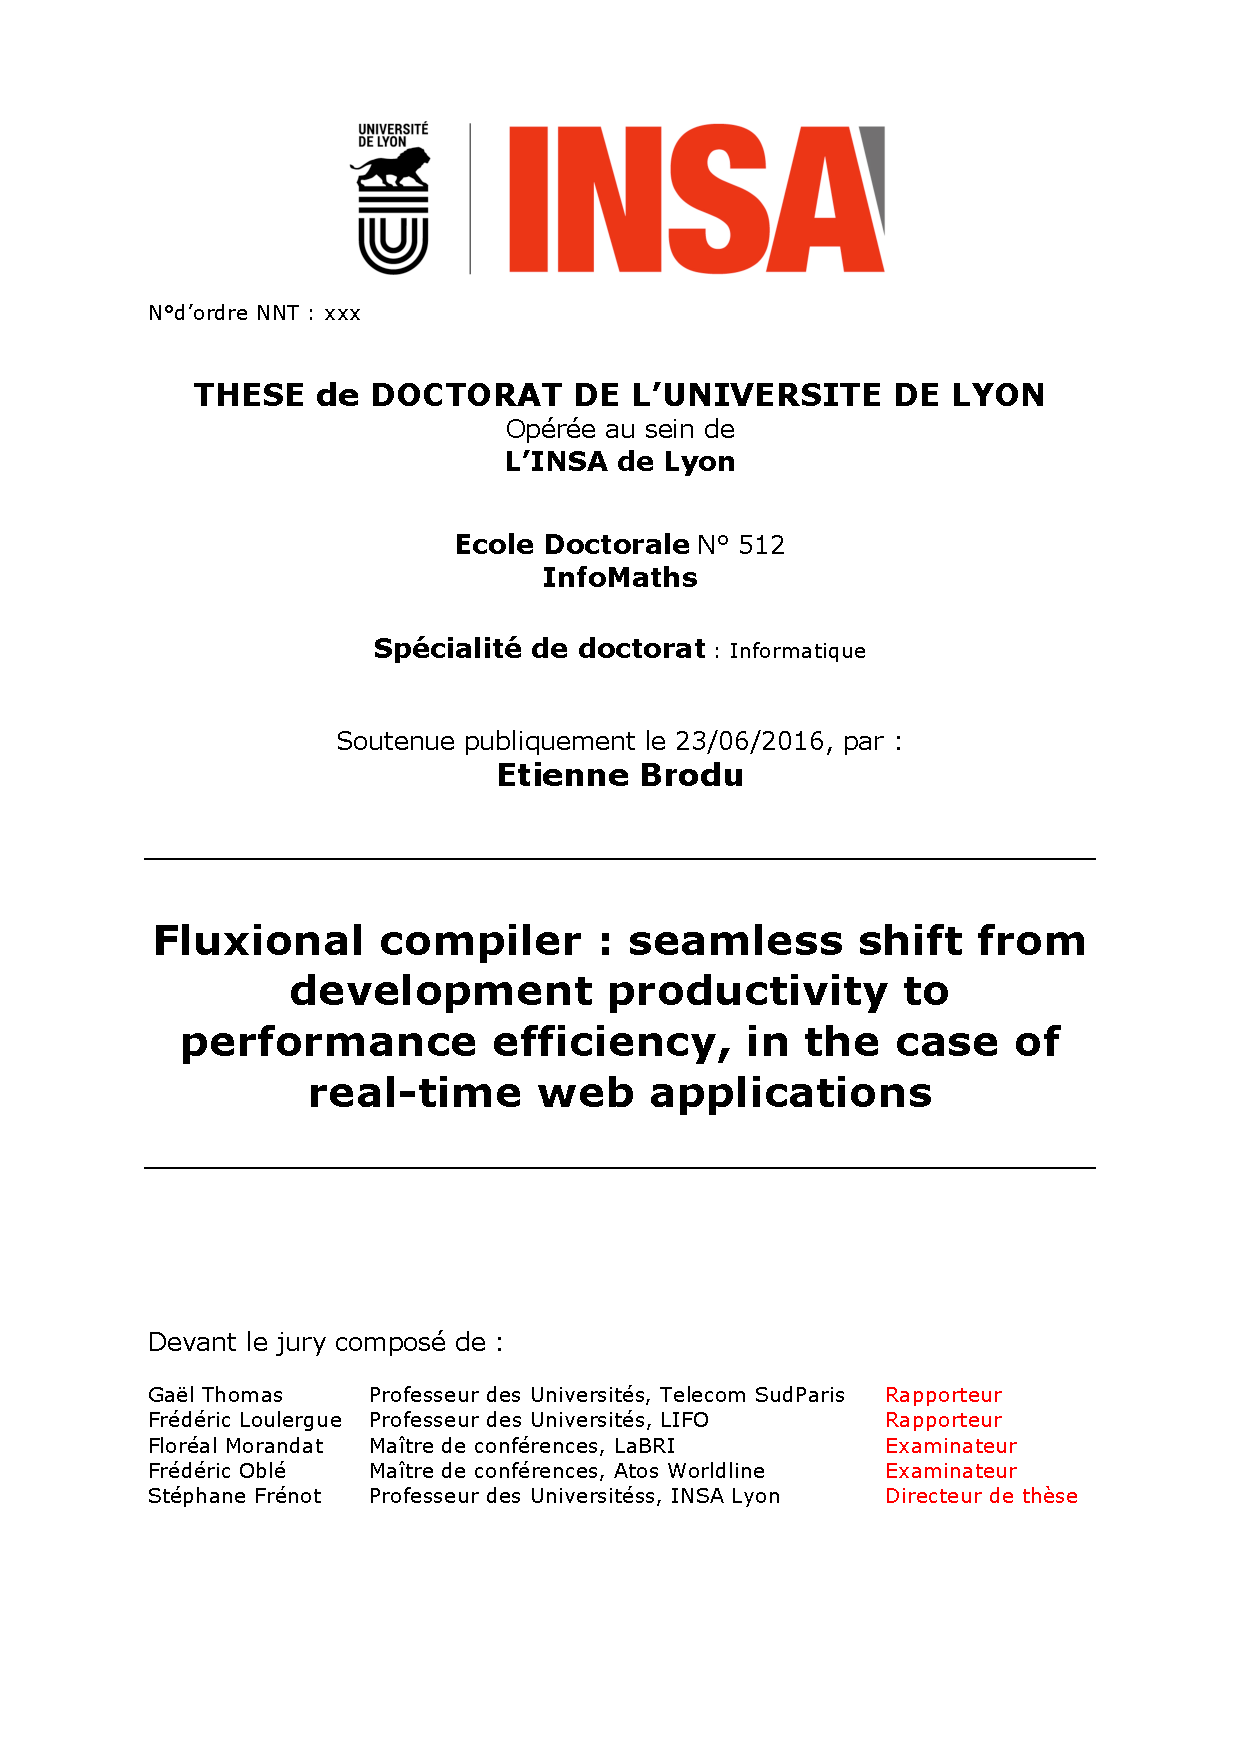
\includepdf{front.pdf} \blank%
\newgeometry{top=1cm, left=2.2cm, right=2.2cm, bottom=1cm}
% \usepackage[top=15mm, bottom=15mm, textwidth=2.4\alphabet, hmarginratio={1:1}]{geometry}
\begin{center}
% \parbox{\linewidth}{%
%   
\includegraphics[height=.4in]{../resources/insa}%
%   \hfill
%   
\includegraphics[height=.4in]{../resources/citi}%
%   \hfill
%   
\includegraphics[height=.4in]{../resources/inria}%
%   \hfill
%   
\includegraphics[height=.4in]{../resources/worldline}%
% }%

\includegraphics[width=8cm]{../resources/logos}%
\\[1em]


{N° d'ordre NNT : xxx \hfill}

\vfill
{
  \fontsize{14pt}{16pt}\selectfont%

  {\large\textbf{\MakeUppercase{Thèse de doctorat de l'université de Lyon}}}\\[1em]

  Opéréé au sein de\\
  {\large\textbf{\MakeUppercase{L'INSA de Lyon}}}\\[1em]

  {\large\textbf{École Doctorale N° }512}\\
  {\large\textbf{\MakeUppercase{InfoMaths}}}\\[1em]

  {\large\textbf{Spécialité de Doctorat : }Informatique}\\[1em]

  Soutenue publiquement le 23/06/2016, par :\\
  {\large\textbf{Etienne Brodu}}\\[1em]
}

\vfill

\parbox{\linewidth}{%
\vspace{10pt}
\titleline%
\vspace{10pt}
\secfont\fontsize{20pt}{25pt}\selectfont%
\MakeUppercase{Fluxional compiler : seamless shift from development productivity to performance efficiency, in the case of real-time web applications}%
\vspace{10pt}%
\titleline\color{black}%
\vspace{10pt}
}

\vfill

Devant le jury composé de : \\[1em]

% \setlength{\tabcolsep}{1em}
% \setlength{\tabrowsep}{0pt}
\begin{tabu} {l X[l] r}
\textbf{Gaël \MakeUppercase{Thomas}}         & Professeur des Universités, Telecom SudParis & Rapporteur\\
\textbf{Frédéric \MakeUppercase{Loulergue}~} & Professeur des Universités, LIFO             & Rapporteur\\
\textbf{Floréal \MakeUppercase{Morandat}}    & Maître de conférences, LaBRI                 & Examinateur\\
\textbf{Frédéric \MakeUppercase{Oblé}}       & Maître de conférences, Atos Worldline        & Examinateur\\
\textbf{Stéphane \MakeUppercase{Frénot}}     & Professeur des Universitéss, INSA Lyon       & Directeur\\
\end{tabu}
\end{center}
\restoregeometry
\eject \blank%
\newgeometry{top=1cm, left=1cm, right=1cm, bottom=1cm}
{%
  \fontsize{13pt}{14pt}\selectfont%
  \noindent\textbf{\hfill Département FEDORA – INSA Lyon - Ecoles Doctorales – Quinquennal 2016-2020\hfill}%
}\vspace{-5pt}
\begingroup\fontsize{9pt}{10pt}\selectfont
\begin{flushleft}
\begin{tabu} {c l X[l]}
\MakeUppercase{sigle} & \MakeUppercase{école doctorale} & \MakeUppercase{nom et coorodonnées du responsable}\\\hline
\textbf{CHIMIE} &%
\parbox[t]{7cm}{%
  \textbf{CHIMIE DE LYON}\\%
  \url{http://www.edchimie-lyon.fr}\\%
  Sec : Renée EL MELHEM\\%
  Bat Blaise Pascal\\%
  3\textsuperscript{e} étage\\%
  \url{secretariat@edchimie-lyon.fr}\\%
  Insa : R. GOURDON
} & \parbox[t]{10cm}{%
  {\fontsize{11pt}{12pt}\selectfont M. Stéphane DANIELE}\\%
  Institut de Recherches sur la Catalyse et l'Environnement de Lyon\\%
  IRCELYON-UMR 5256\\%
  Équipe CDFA\\%
  2 avenue Albert Einstein\\%
  69626 Villeurbanne cedex\\%
  \url{directeur@edchimie-lyon.fr}
}\\\hline%
\textbf{E.E.A.} &%
\parbox[t]{7cm}{%
  \textbf{ELECTRONIQUE, ELECTROTECHNIQUE, AUTOMATIQUE}\\%
  \url{http://edeea.ec-lyon.fr}\\%
  Sec : M.C. HAVGOUDOUKIAN\\%
  \url{Ecole-Doctorale.eea@ec-lyon.fr}
} & \parbox[t]{6cm}{
  {\fontsize{11pt}{12pt}\selectfont M. Gérard SCORLETTI}\\%
  Ecole Centrale de Lyon\\%
  36 avenue Guy de Collongue\\%
  69134 ECULLY \\%
  Tél : 04 72 18 60 97 Fax : 04 78 43 37 17\\%
  \url{Gerard.scorletti@ec-lyon.fr}
}\\\hline%
\textbf{E2M2} &%
\parbox[t]{7cm}{%
  \textbf{EVOLUTION, ECOSYSTEME, MICROBIOLOGIE, MODELISATION}\\%
  \url{http ://e2m2.universite-lyon.fr}\\%
  Sec : Safia AIT CHALAL\\%
  Bat Darwin -UCB Lyon 1\\%
  Tél : 04 72 43 28 91\\%
  Insa : H. CHARLES\\%
  \url{Safia.ait-chalal@univ-lyon1.fr}
} & \parbox[t]{6cm}{
  {\fontsize{11pt}{12pt}\selectfont Mme Gudrun BORNETTE}\\%
  CNRS UMR 5023 LEHNA\\%
  Université Claude Bernard Lyon 1\\%
  Bât Forel\\%
  43 bd du 11 novembre 1918\\%
  69622 VILLEURBANNE Cédex\\%
  Tél : 06 07 53 89 13\\%
  \url{e2m2@univ-lyon1.fr}
}\\\hline%
\textbf{EDISS} &%
\parbox[t]{7cm}{%
  \textbf{INTERDISCIPLINAIRE SCIENCES-SANTE}\\%
  \url{http://www.ediss-lyon.fr}\\%
  Sec : Safia AIT CHALAL\\%
  Hôpital Louis Pradel -Bron\\%
  Tél : 04 72 68 49 09\\%
  Insa : M. LAGARDE\\%
  \url{Safia.ait-chalal@univ-lyon1.fr}
} & \parbox[t]{10cm}{%
  {\fontsize{11pt}{12pt}\selectfont Mme Emmanuelle CANET-SOULAS}\\%
  INSERM U1060, CarMeN lab, Univ. Lyon 1 \\%
  Bâtiment IMBL\\%
  11 avenue Jean Capelle INSA de Lyon\\%
  69621 Villeurbanne\\%
  Tél : 04 72 68 49 09 Fax : 04 72 68 49 16\\%
  \url{Emmanuelle.canet@univ-lyon1.fr}
}\\\hline%
\textbf{INFOMATHS} &%
\parbox[t]{7cm}{%
  \textbf{INFORMATIQUE ET MATHEMATIQUES}\\%
  \url{http://infomaths.univ-lyon1.fr}\\%
  Sec : Renée EL MELHEM\\%
  Bat Blaise Pascal\\%
  3\textsuperscript{e} étage\\%
  \url{infomaths@univ-lyon1.fr}
} & \parbox[t]{10cm}{%
  {\fontsize{11pt}{12pt}\selectfont Mme Sylvie CALABRETTO}\\%
  LIRIS – INSA de Lyon\\%
  Bat Blaise Pascal\\%
  7 avenue Jean Capelle\\%
  69622 VILLEURBANNE Cedex\\%
  Tél : 04 72 43 80 46 Fax 04 72 43 16 87\\%
  \url{Sylvie.calabretto@insa-lyon.fr}
}\\\hline%
\textbf{Matériaux} &%
\parbox[t]{7cm}{%
  \textbf{MATERIAUX DE LYON}\\%
  \url{http://ed34.universite-lyon.fr}\\%
  Sec : M. LABOUNE\\%
  PM : 71 70 Fax : 87 12 \\%
  Bat. Saint Exupéry\\%
  \url{Ed.materiaux@insa-lyon.fr}%
} & \parbox[t]{10cm}{%
  {\fontsize{11pt}{12pt}\selectfont M. Jean-Yves BUFFIERE}\\%
  INSA de Lyon\\%
  MATEIS\\%
  Bâtiment Saint Exupéry\\%
  7 avenue Jean Capelle\\%
  69621 VILLEURBANNE Cedex\\%
  Tél : 04 72 43 71 70 Fax 04 72 43 85 28\\%
  \url{Ed.materiaux@insa-lyon.fr}
}\\\hline%
\textbf{MEGA} &%
\parbox[t]{7cm}{%
  \textbf{MECANIQUE, ENERGETIQUE, GENIE CIVIL, ACOUSTIQUE}\\%
  \url{http://mega.universite-lyon.fr}\\%
  Sec : M. LABOUNE\\%
  PM : 71 70 Fax : 87 12 \\%
  Bat. Saint Exupéry\\%
  \url{mega@insa-lyon.fr}%
} & \parbox[t]{10cm}{%
  {\fontsize{11pt}{12pt}\selectfont M. Philippe BOISSE}\\%
  INSA de Lyon\\%
  Laboratoire LAMCOS\\%
  Bâtiment Jacquard\\%
  25 bis avenue Jean Capelle\\%
  69621 VILLEURBANNE Cedex\\%
  Tél : 04 72 43 71 70 Fax : 04 72 43 72 37\\%
  \url{Philippe.boisse@insa-lyon.fr}
}\\\hline%
\textbf{ScSo} &%
\parbox[t]{7cm}{%
  \textbf{ScSo}\footnote{ScSo : Histoire, Géographie, Aménagement, Urbanisme, Archéologie, Science politique, Sociologie, Anthropologie}\\%
  \url{http://recherche.univ-lyon2.fr/scso/}\\%
  Sec : Viviane POLSINELLI, Brigitte DUBOIS\\%
  Insa : J.Y. TOUSSAINT\\%
  \url{viviane.polsinelli@univ-lyon2.fr}%
} & \parbox[t]{10cm}{%
  {\fontsize{11pt}{12pt}\selectfont Mme Isabelle VON BUELTZINGLOEWEN}\\%
  Université Lyon 2\\%
  86 rue Pasteur\\%
  69365 LYON Cedex 07\\%
  Tél : 04 78 77 23 86 Fax : 04 37 28 04 48%
}%
\end{tabu}
\end{flushleft}
\endgroup
\restoregeometry
\eject  \blank%

\renewcommand{\glyph}{\iconfont{\XeTeXglyph287}}
\chapter{Implementations} \label{chapter5}
\minitoc
\eject
The transformation allowed by the equivalence from an event-driven program into a distributed network of fluxions is implemented incrementally into two compilers, as presented in figure \ref{fig:roadmap}.
Each compilers is divided into two steps, the identification of the rupture points separating the stages of the pipeline, and the isolation of these stages.
% This chapter presents the technical implementations of these two steps in the transformation from the event-driven execution model to the pipeline architecture
% , the transformation described in the previous chapter was implemented incrementally in two compilers.

\begin{figure}[h!]%
  \textfig{%
    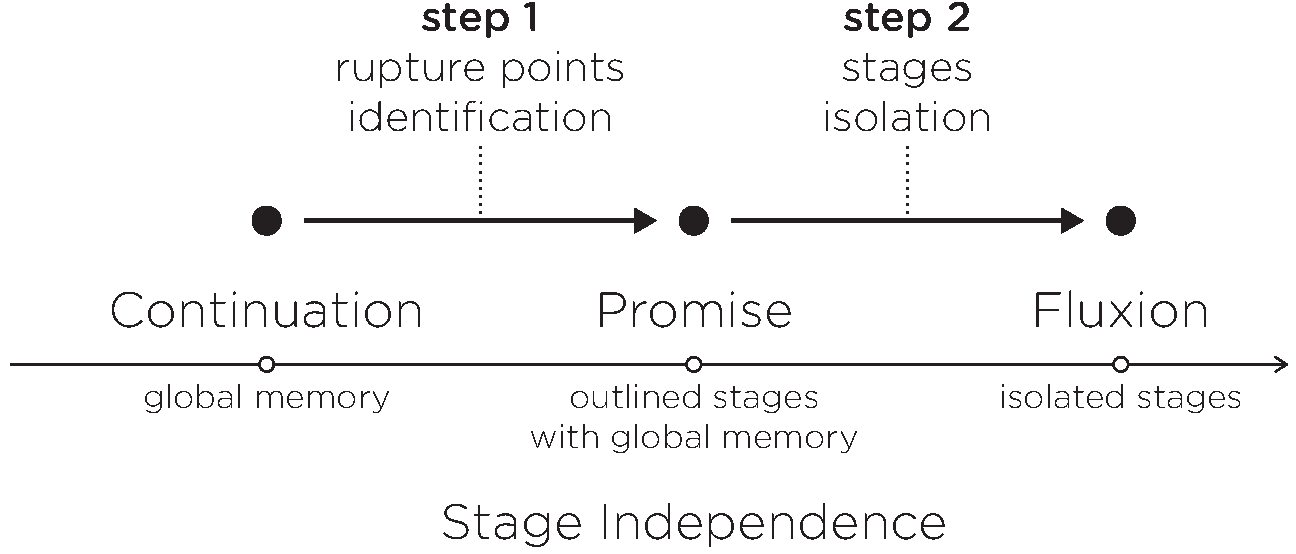
\includegraphics[width=0.7\textwidth]{../resources/roadmap.pdf}%
    \caption{Roadmap}%
    \label{fig:roadmap}%
  }%
\end{figure}

The first compiler focuses on the identification of simple chains of causality between continuations to transform these chains into Promises.
% the transformation from continuations to Promises.
% It focuses on the identification of the chains of causality in continuations.
However, promises are more expressive than the simple chaining of causal sequentiality.
% They force another control over the execution flow.
% According to the outcome of the operation, they call one function to continue the execution with the result, or another to handle errors.
% This conditional execution is indivisible from the Promise specification.
% Promises impose a convention on how to hand back the outcome of the deferred computation, while classic continuations leave this conditional execution to the developer.
Moreover, they impose a different convention than continuations on how to hand back the outcome and errors of the deferred computation.
This difference brings unnecessary complexity to the identification of chains.
To rule out this difference between continuations and Promises, before introducing the first compiler, section \ref{chapter5:due} introduces a simpler specification to Promise, called Due.

The second compiler detects all the chains of causality between continuations and encapsulate them in fluxions.
It isolates the fluxions when possible to allow the parallelism required for efficiency.
This second compilers is introduced in section \ref{chapter5:flx}.

\renewcommand{\glyph}{\iconfont{\XeTeXglyph287}}
\chapter{Implementations} \label{chapter5}
\minitoc
\eject
The transformation allowed by the equivalence from an event-driven program into a distributed network of fluxions is implemented incrementally into two compilers, as presented in figure \ref{fig:roadmap}.
Each compilers is divided into two steps, the identification of the rupture points separating the stages of the pipeline, and the isolation of these stages.
% This chapter presents the technical implementations of these two steps in the transformation from the event-driven execution model to the pipeline architecture
% , the transformation described in the previous chapter was implemented incrementally in two compilers.

\begin{figure}[h!]%
  \textfig{%
    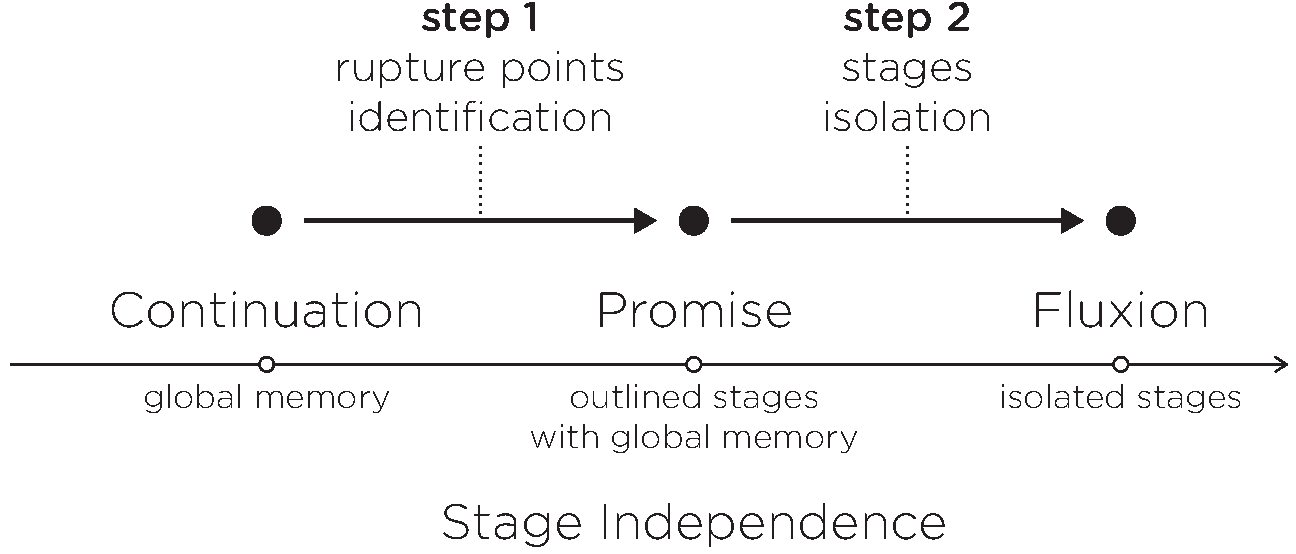
\includegraphics[width=0.7\textwidth]{../resources/roadmap.pdf}%
    \caption{Roadmap}%
    \label{fig:roadmap}%
  }%
\end{figure}

The first compiler focuses on the identification of simple chains of causality between continuations to transform these chains into Promises.
% the transformation from continuations to Promises.
% It focuses on the identification of the chains of causality in continuations.
However, promises are more expressive than the simple chaining of causal sequentiality.
% They force another control over the execution flow.
% According to the outcome of the operation, they call one function to continue the execution with the result, or another to handle errors.
% This conditional execution is indivisible from the Promise specification.
% Promises impose a convention on how to hand back the outcome of the deferred computation, while classic continuations leave this conditional execution to the developer.
Moreover, they impose a different convention than continuations on how to hand back the outcome and errors of the deferred computation.
This difference brings unnecessary complexity to the identification of chains.
To rule out this difference between continuations and Promises, before introducing the first compiler, section \ref{chapter5:due} introduces a simpler specification to Promise, called Due.

The second compiler detects all the chains of causality between continuations and encapsulate them in fluxions.
It isolates the fluxions when possible to allow the parallelism required for efficiency.
This second compilers is introduced in section \ref{chapter5:flx}.

\renewcommand{\glyph}{\iconfont{\XeTeXglyph287}}
\chapter{Implementations} \label{chapter5}
\minitoc
\eject
The transformation allowed by the equivalence from an event-driven program into a distributed network of fluxions is implemented incrementally into two compilers, as presented in figure \ref{fig:roadmap}.
Each compilers is divided into two steps, the identification of the rupture points separating the stages of the pipeline, and the isolation of these stages.
% This chapter presents the technical implementations of these two steps in the transformation from the event-driven execution model to the pipeline architecture
% , the transformation described in the previous chapter was implemented incrementally in two compilers.

\begin{figure}[h!]%
  \textfig{%
    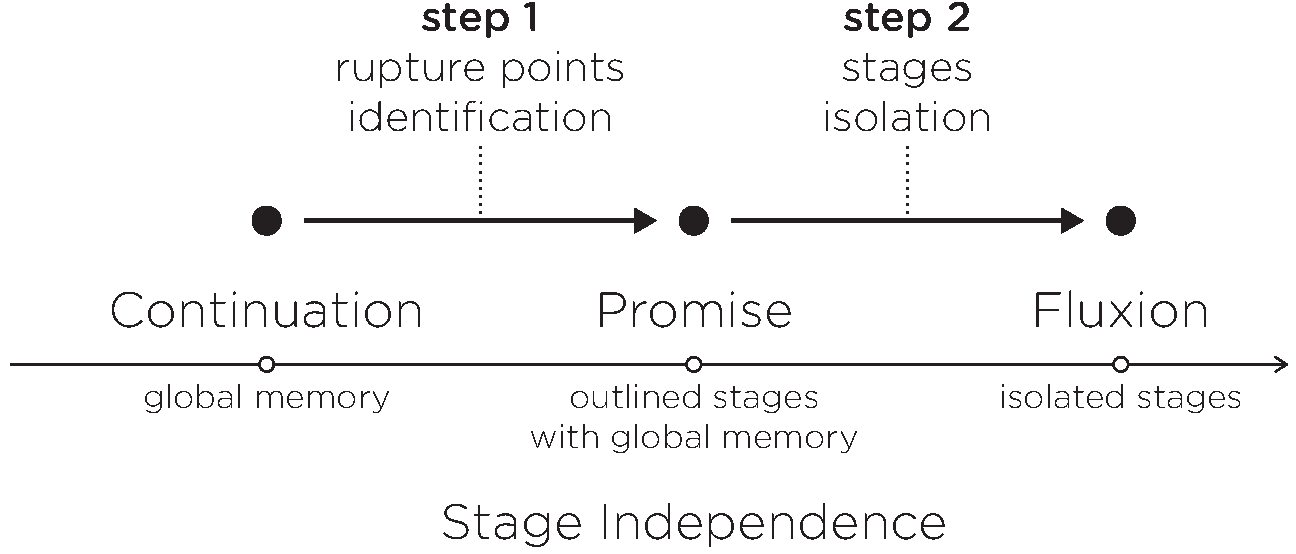
\includegraphics[width=0.7\textwidth]{../resources/roadmap.pdf}%
    \caption{Roadmap}%
    \label{fig:roadmap}%
  }%
\end{figure}

The first compiler focuses on the identification of simple chains of causality between continuations to transform these chains into Promises.
% the transformation from continuations to Promises.
% It focuses on the identification of the chains of causality in continuations.
However, promises are more expressive than the simple chaining of causal sequentiality.
% They force another control over the execution flow.
% According to the outcome of the operation, they call one function to continue the execution with the result, or another to handle errors.
% This conditional execution is indivisible from the Promise specification.
% Promises impose a convention on how to hand back the outcome of the deferred computation, while classic continuations leave this conditional execution to the developer.
Moreover, they impose a different convention than continuations on how to hand back the outcome and errors of the deferred computation.
This difference brings unnecessary complexity to the identification of chains.
To rule out this difference between continuations and Promises, before introducing the first compiler, section \ref{chapter5:due} introduces a simpler specification to Promise, called Due.

The second compiler detects all the chains of causality between continuations and encapsulate them in fluxions.
It isolates the fluxions when possible to allow the parallelism required for efficiency.
This second compilers is introduced in section \ref{chapter5:flx}.

\input{05-implementation/Due/main}
\input{05-implementation/Flx/main}
% \input{05-implementation/Evaluation}

\renewcommand{\glyph}{\iconfont{\XeTeXglyph287}}
\chapter{Implementations} \label{chapter5}
\minitoc
\eject
The transformation allowed by the equivalence from an event-driven program into a distributed network of fluxions is implemented incrementally into two compilers, as presented in figure \ref{fig:roadmap}.
Each compilers is divided into two steps, the identification of the rupture points separating the stages of the pipeline, and the isolation of these stages.
% This chapter presents the technical implementations of these two steps in the transformation from the event-driven execution model to the pipeline architecture
% , the transformation described in the previous chapter was implemented incrementally in two compilers.

\begin{figure}[h!]%
  \textfig{%
    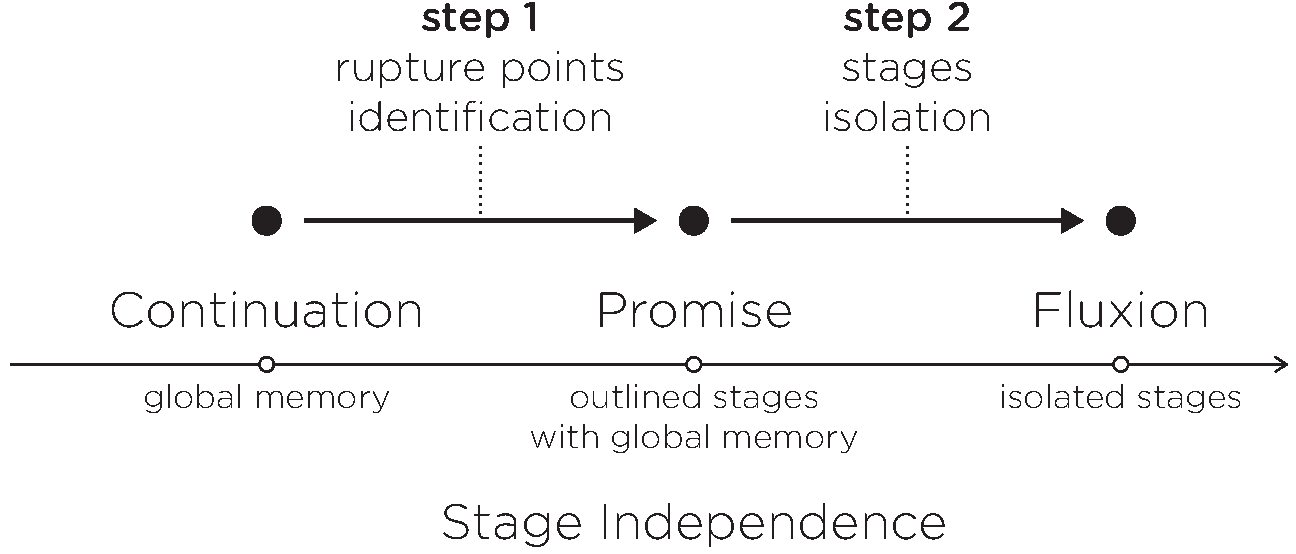
\includegraphics[width=0.7\textwidth]{../resources/roadmap.pdf}%
    \caption{Roadmap}%
    \label{fig:roadmap}%
  }%
\end{figure}

The first compiler focuses on the identification of simple chains of causality between continuations to transform these chains into Promises.
% the transformation from continuations to Promises.
% It focuses on the identification of the chains of causality in continuations.
However, promises are more expressive than the simple chaining of causal sequentiality.
% They force another control over the execution flow.
% According to the outcome of the operation, they call one function to continue the execution with the result, or another to handle errors.
% This conditional execution is indivisible from the Promise specification.
% Promises impose a convention on how to hand back the outcome of the deferred computation, while classic continuations leave this conditional execution to the developer.
Moreover, they impose a different convention than continuations on how to hand back the outcome and errors of the deferred computation.
This difference brings unnecessary complexity to the identification of chains.
To rule out this difference between continuations and Promises, before introducing the first compiler, section \ref{chapter5:due} introduces a simpler specification to Promise, called Due.

The second compiler detects all the chains of causality between continuations and encapsulate them in fluxions.
It isolates the fluxions when possible to allow the parallelism required for efficiency.
This second compilers is introduced in section \ref{chapter5:flx}.

\input{05-implementation/Due/main}
\input{05-implementation/Flx/main}
% \input{05-implementation/Evaluation}

% \subsection{Real test case} \label{chapter5:flx:evaluation}

The compiler is tested on a real application, gifsockets-server\ftnt{https://github.com/twolfson/gifsockets-server}.
This test proves the possibility for an application to be compiled into a network of independent parts.
It shows the current limitations of this isolation and the modifications needed on the application to circumvent them.

\begin{code}[js, caption={Simplified version of gifsockets-server},label={lst:gifsocket}]
var express = require('express'),
    app = express(),
    routes = require('gifsockets-middleware'), //@\label{lst:gifsocket:gif-mw}@
    getRawBody = require('raw-body');

function bodyParser(limit) { //@\label{lst:gifsocket:bodyParser}@
  return function saveBody(req, res, next) { //@\label{lst:gifsocket:saveBody}@
    getRawBody(req, { //@\label{lst:gifsocket:getRawBody}@
      expected: req.headers['content-length'],
      limit: limit
    }, function (err, buffer) { //@\label{lst:gifsocket:callback}@
      req.body = buffer;
      next(); //@\label{lst:gifsocket:next}@
    });
  };
}

app.post('/image/text', bodyParser(1 * 1024 * 1024), routes.writeTextToImages); //@\label{lst:gifsocket:app.post}@
app.listen(8000);
\end{code}

This application, simplified in listing \ref{lst:gifsocket}, is a real-time chat using gif-based communication channels.
It was selected from the evaluation set of the Due compiler because it is simple enough to illustrate this evaluation.
% \cite{Brodu2015}
%  from the \texttt{npm} registry because it depends on \texttt{express}, it is tested, working, and simple enough to illustrate this evaluation.
The server transforms the received text into a gif frame, and pushes it back to a never-ending gif to be displayed on the client.

On line \ref{lst:gifsocket:app.post}, the application registers two functions to process the requests received on the url \texttt{/image/text}.
The closure \texttt{saveBody}, line \ref{lst:gifsocket:saveBody}, returned by \texttt{bodyParser}, line \ref{lst:gifsocket:bodyParser}, and the method \texttt{routes.write\-Text\-To\-Images} from the external module \texttt{gifsockets-\-middleware}, line \ref{lst:gifsocket:gif-mw}.
The closure \texttt{saveBody} calls the asynchronous function \texttt{getRawBody} to get the request body.
Its callback handles the errors, and calls \texttt{next} to continue processing the request with the next function, \texttt{routes.write\-Text\-To\-Images}.

\subsubsection{Compilation} \label{chapter5:flx:evaluation:compilation}

% We compile this application with the compiler
The compilation result is in listing \ref{lst:flx-gifsocket}.
The function call \texttt{app.post}, line \ref{lst:gifsocket:app.post}, is a rupture point.
However, its callbacks, \texttt{bodyParser} and \texttt{routes.write\-Text\-To\-Images} are not declared \textit{in situ}.
They are evaluated as functions only at runtime.
As precised previously, the compiler discards these callbacks to avoid altering the semantic. % by moving or modifying their definition.
% For this reason, the compiler ignores this rupture point, to avoid interfering with the evaluation.

\begin{code}[flx, caption={Compilation result of gifsockets-server},label={lst:flx-gifsocket}]
flx main & express {req}
>> anonymous_1000 [req, next]
  var express = require('express'),
      app = express(),
      routes = require('gifsockets-middleware'), //@\label{lst:flx-gifsocket:gif-mw}@
      getRawBody = require('raw-body');

  function bodyParser(limit) { //@\label{lst:flx-gifsocket:bodyParser}@
    return function saveBody(req, res, next) { //@\label{lst:flx-gifsocket:saveBody}@
      getRawBody(req, { //@\label{lst:flx-gifsocket:getRawBody}@
        expected: req.headers['content-length'], //@\label{lst:flx-gifsocket:req.headers}@
        limit: limit
      }, >> anonymous_1000 [req, next]);
    };
  }

  app.post('/image/text', bodyParser(1 * 1024 * 1024), routes.writeTextToImages); //@\label{lst:flx-gifsocket:app.post}@
  app.listen(8000);

flx anonymous_1000
-> null
  function (err, buffer) { //@\label{lst:flx-gifsocket:callback}@
    req.body = buffer; //@\label{lst:flx-gifsocket:buffer}@
    next(); //@\label{lst:flx-gifsocket:next}@
  }
\end{code}

The compiler detects a rupture point : the function \texttt{get\-Raw\-Body} and its anonymous callback, line \ref{lst:gifsocket:callback}.
It encapsulates this callback in a fluxion named \texttt{anony\-mous\_\-1000}.
The callback is replaced with a stream placeholder to send the message stream to this downstream fluxion.
The variables \texttt{req} and \texttt{next} are appended to this message stream, to propagate their value from the \texttt{main} fluxion to the \texttt{anony\-mous\_\-1000} fluxion.

When \texttt{anony\-mous\_\-1000} is not isolated from the \texttt{main} fluxion, as if they belong to the same group, the compilation result works as expected.
The variables used in the fluxion, \texttt{req} and \texttt{next}, are still shared between the two fluxions.
In this situation fluxions are quite similar to Dues regarding memory shareing.
Our goal is to isolate the two fluxions, to be able to safely parallelize their executions.

\subsubsection{Isolation} \label{chapter5:flx:evaluation:isolation}

In listing \ref{lst:flx-gifsocket}, the fluxion \texttt{anony\-mous\_\-1000} modifies the object \texttt{req}, line \ref{lst:flx-gifsocket:buffer}, to store the text of the received request, and it calls \texttt{next} to continue the execution, line \ref{lst:flx-gifsocket:next}.
\texttt{req} is an alias to a memory location used in multiple palces in code.
Therefore, these operations produce side-effects that should propagate in the whole application, but the isolation prevents this propagation.
Isolating the fluxion \texttt{anony\-mous\_\-1000} produces runtime exceptions.
The next paragraph details how this situation is handled to allow the application to be parallelized.

\paragraph{Variable \texttt{req}}

The variable \texttt{req} is read in fluxion \texttt{main}, lines \ref{lst:flx-gifsocket:getRawBody} and \ref{lst:flx-gifsocket:req.headers}.
Then its property \texttt{body} is associated to \texttt{buffer} in fluxion \texttt{anony\-mous\_\-1000}, line \ref{lst:flx-gifsocket:buffer}.
The compiler is unable to identify the aliases of this variable. % further usages.
However, the side effect resulting from this association impacts a variable in the scope of the next callback, \texttt{routes.write\-Text\-To\-Images}.
In this test case, the application is modified manually to explicitly propagate this side-effect to the next callback through the function \texttt{next}.
The modifications of this function are explained further in the next paragraph.

\paragraph{Closure \texttt{next}}

The function \texttt{next} is a closure provided by the \texttt{express} \texttt{Router} to continue the execution with the next function to handle the client request.
Because it indirectly relies on the variable \texttt{req}, it is impossible to isolate its execution with the \texttt{anony\-mous\_\-1000} fluxion.
Instead, we modify \texttt{express}, so as to be compatible with the fluxional execution model.
We explain the modifications below.

\begin{code}[flx, caption={Simplified modification on the compiled result},label={lst:mflx-gifsocket}]
flx anonymous_1000
-> express_dispatcher
  function (err, buffer) { //@\label{lst:mflx-gifsocket:callback}@
    req.body = buffer; //@\label{lst:mflx-gifsocket:buffer}@
    next_placeholder(req, -> express_dispatcher); //@\label{lst:mflx-gifsocket:next-placeholder}@
  }

flx express_dispatcher & express {req} //@\label{lst:mflx-gifsocket:express-dispatcher}@
-> null
  function (modified_req) {
    merge(req, modified_req);
    next(); //@\label{lst:mflx-gifsocket:next}@
  }
\end{code}

In listing \ref{lst:gifsocket}, the function \texttt{next} is a continuation allowing the anonymous callback, line \ref{lst:gifsocket:callback}, to call the next function to handle the request.
To isolate the anonymous callback into \texttt{anonymous\_\-1000}, \texttt{next} is replaced by a rupture point.
This replacement is illustrated in listing \ref{lst:mflx-gifsocket}.
The \texttt{express} \texttt{Router} registers a fluxion named \texttt{express\_\-dispatcher}, line \ref{lst:mflx-gifsocket:express-dispatcher}, to continue the execution after the fluxion \texttt{anony\-mous\_\-1000}.
This fluxion is in the same group \texttt{express} as the \texttt{main} fluxion, hence it has access to the original variable \texttt{req}, and to the original function \texttt{next}.
The call to the original \texttt{next} function is replaced by a placeholder to push the stream to the fluxion \texttt{express\_\-dispatcher}, line \ref{lst:mflx-gifsocket:next-placeholder}.
The fluxion \texttt{express\_\-dispatcher} receives the stream from the upstream fluxion \texttt{anony\-mous\_\-1000}, merges back the modification in the variable \texttt{req} to propagate the side effects, and finally calls the original function \texttt{next} to continue the execution, line \ref{lst:mflx-gifsocket:next}.

After the modifications detailed above, the server works as expected.
The isolated fluxion correctly receives, and returns its serialized messages.
The client successfully receives a gif frame containing the text.



\subsection{Limitations}

The static analysis used for this compiler presents some limitations.
It is unable to analyze code with dynamic behaviors.
Higher-order programming leads to more productivity partly beacuse it rely on such dynamic behavior to extend expressivity.
Precisely, it allows more levels of indirections.

\subsubsection{Levels of Indirections}

The indirection is an abstraction between the value, and its manipulation.
In listing \ref{lst:indirection}, the variables \texttt{a} and \texttt{b} point both to the same memory object.
The function \texttt{fn} introduces a level of indirection between the real object \texttt{a} and its manipulation handle, \texttt{b};
% Actually, the variable \texttt{a} already introduces a level of indirection between the real object and the handle \texttt{a}.

\begin{code}[js,
  caption={One level of Indirection},
  label={lst:indirection}]
var a = {
      // an object;
    };

fn(b) {
  // modify b;
}

fn(a);
\end{code}

\subsubsection{Uncertainties}

The indirection is trivial to resolve in listing \ref{lst:indirection}.
It only needs to have access to the definition of \texttt{a} and of \texttt{fn}.
%A very simple static analysis could resolve it.
However, in listing \ref{lst:indirections}, the array \texttt{handlers} introduces a new level of indirection.
The static analysis now needs to have access to the definition of \texttt{i} and of the \texttt{handlers}.
If this definition is provided by an external input, it is not available statically, hence, it adds an uncertainty during the analysis. 

\begin{code}[js,
  caption={Two levels of indirection},
  label={lst:indirections}]
var a = {
      // an object;
    },
    handlers = [
      // definition of fn handlers;
    ],
    i = ?;

handlers[i](a);
handlers[i+1](a);
\end{code}

These examples are extremely simplified.
A real application contains enough indirections for the static analysis to be overwhelmed by uncertainties, and to be unable to resolve the variables.
If a variable is left unresolved, it is impossible to assure its scope and its aliases.
Therefore, the compiler is unable to isolate it into a fluxion, or to distribute its modification by messages.

Moreover, it leads the compiler to ignore the rupture points not defined \textit{in situ}, because their modifications could impact the semantic.
The reason for this precaution, is that the compiler is unable to assure where the function is used, and the scope of its variables.
Therefore, it is unable to assure that the modification will conserve the semantic.

\subsubsection{Dynamic Resolution}

In a web application, this variable \texttt{i} might be part of the user request, which is available only at runtime.
It eventually introduces an uncertainty.

This dynamic resolution of variables is precisely what increase expressiveness.
Trying to resolve them statically is equivalent to restrict expressiveness.
No static analysis can overstep these limitations.
Only a dynamic analysis could analysis the resolved indirections during run time to overstep these limitations correctly.




\renewcommand{\glyph}{\iconfont{\XeTeXglyph287}}
\chapter{Implementations} \label{chapter5}
\minitoc
\eject
The transformation allowed by the equivalence from an event-driven program into a distributed network of fluxions is implemented incrementally into two compilers, as presented in figure \ref{fig:roadmap}.
Each compilers is divided into two steps, the identification of the rupture points separating the stages of the pipeline, and the isolation of these stages.
% This chapter presents the technical implementations of these two steps in the transformation from the event-driven execution model to the pipeline architecture
% , the transformation described in the previous chapter was implemented incrementally in two compilers.

\begin{figure}[h!]%
  \textfig{%
    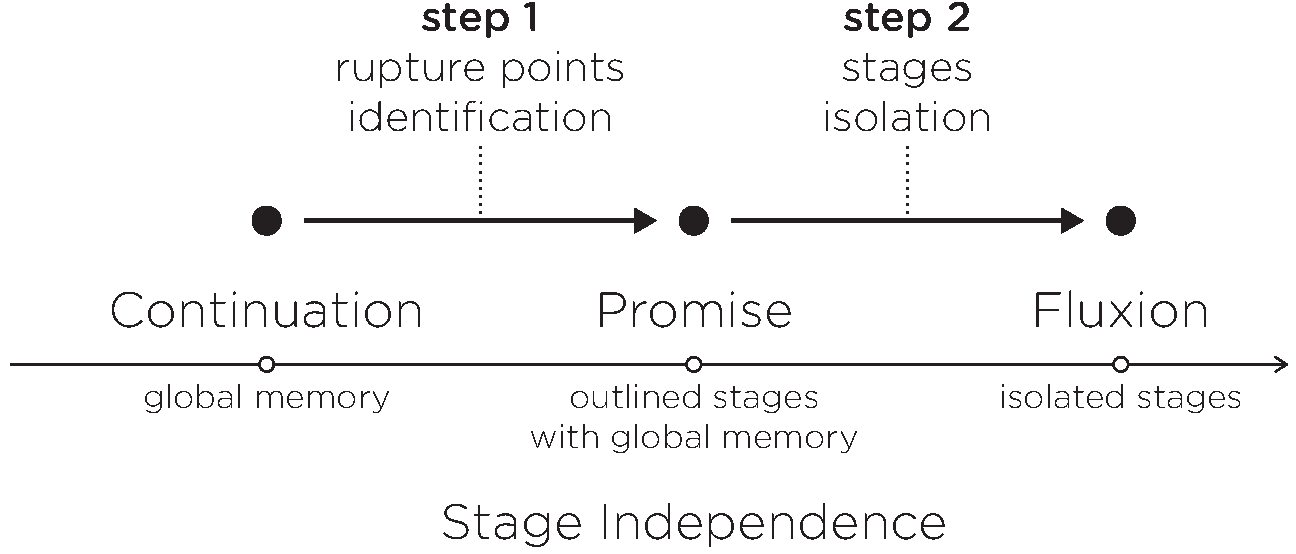
\includegraphics[width=0.7\textwidth]{../resources/roadmap.pdf}%
    \caption{Roadmap}%
    \label{fig:roadmap}%
  }%
\end{figure}

The first compiler focuses on the identification of simple chains of causality between continuations to transform these chains into Promises.
% the transformation from continuations to Promises.
% It focuses on the identification of the chains of causality in continuations.
However, promises are more expressive than the simple chaining of causal sequentiality.
% They force another control over the execution flow.
% According to the outcome of the operation, they call one function to continue the execution with the result, or another to handle errors.
% This conditional execution is indivisible from the Promise specification.
% Promises impose a convention on how to hand back the outcome of the deferred computation, while classic continuations leave this conditional execution to the developer.
Moreover, they impose a different convention than continuations on how to hand back the outcome and errors of the deferred computation.
This difference brings unnecessary complexity to the identification of chains.
To rule out this difference between continuations and Promises, before introducing the first compiler, section \ref{chapter5:due} introduces a simpler specification to Promise, called Due.

The second compiler detects all the chains of causality between continuations and encapsulate them in fluxions.
It isolates the fluxions when possible to allow the parallelism required for efficiency.
This second compilers is introduced in section \ref{chapter5:flx}.

\renewcommand{\glyph}{\iconfont{\XeTeXglyph287}}
\chapter{Implementations} \label{chapter5}
\minitoc
\eject
The transformation allowed by the equivalence from an event-driven program into a distributed network of fluxions is implemented incrementally into two compilers, as presented in figure \ref{fig:roadmap}.
Each compilers is divided into two steps, the identification of the rupture points separating the stages of the pipeline, and the isolation of these stages.
% This chapter presents the technical implementations of these two steps in the transformation from the event-driven execution model to the pipeline architecture
% , the transformation described in the previous chapter was implemented incrementally in two compilers.

\begin{figure}[h!]%
  \textfig{%
    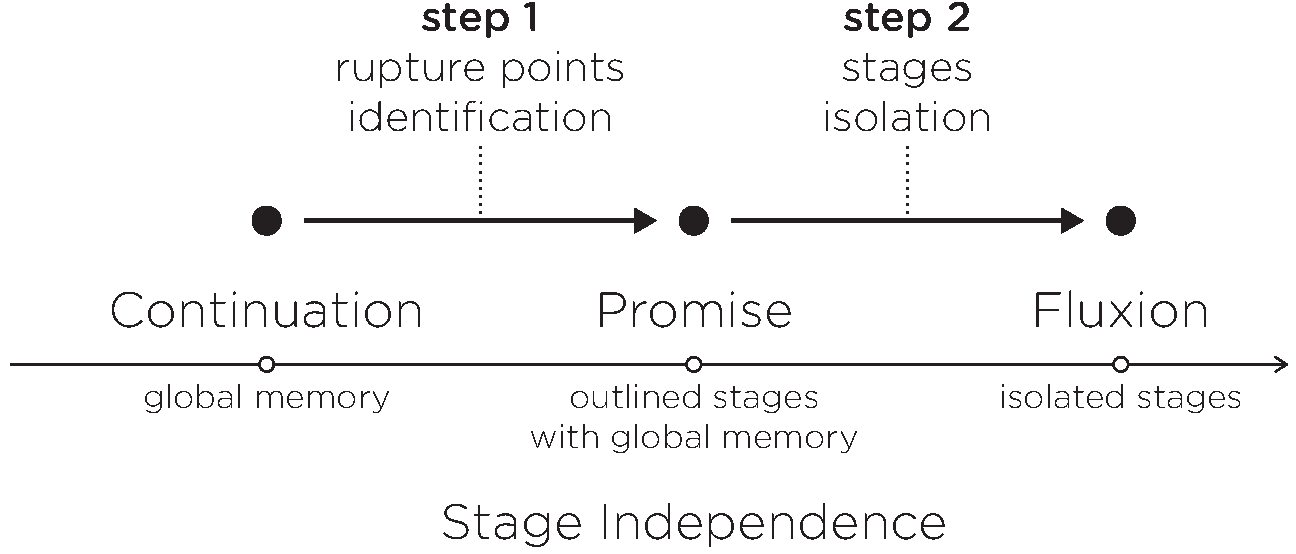
\includegraphics[width=0.7\textwidth]{../resources/roadmap.pdf}%
    \caption{Roadmap}%
    \label{fig:roadmap}%
  }%
\end{figure}

The first compiler focuses on the identification of simple chains of causality between continuations to transform these chains into Promises.
% the transformation from continuations to Promises.
% It focuses on the identification of the chains of causality in continuations.
However, promises are more expressive than the simple chaining of causal sequentiality.
% They force another control over the execution flow.
% According to the outcome of the operation, they call one function to continue the execution with the result, or another to handle errors.
% This conditional execution is indivisible from the Promise specification.
% Promises impose a convention on how to hand back the outcome of the deferred computation, while classic continuations leave this conditional execution to the developer.
Moreover, they impose a different convention than continuations on how to hand back the outcome and errors of the deferred computation.
This difference brings unnecessary complexity to the identification of chains.
To rule out this difference between continuations and Promises, before introducing the first compiler, section \ref{chapter5:due} introduces a simpler specification to Promise, called Due.

The second compiler detects all the chains of causality between continuations and encapsulate them in fluxions.
It isolates the fluxions when possible to allow the parallelism required for efficiency.
This second compilers is introduced in section \ref{chapter5:flx}.

\input{05-implementation/Due/main}
\input{05-implementation/Flx/main}
% \input{05-implementation/Evaluation}

\renewcommand{\glyph}{\iconfont{\XeTeXglyph287}}
\chapter{Implementations} \label{chapter5}
\minitoc
\eject
The transformation allowed by the equivalence from an event-driven program into a distributed network of fluxions is implemented incrementally into two compilers, as presented in figure \ref{fig:roadmap}.
Each compilers is divided into two steps, the identification of the rupture points separating the stages of the pipeline, and the isolation of these stages.
% This chapter presents the technical implementations of these two steps in the transformation from the event-driven execution model to the pipeline architecture
% , the transformation described in the previous chapter was implemented incrementally in two compilers.

\begin{figure}[h!]%
  \textfig{%
    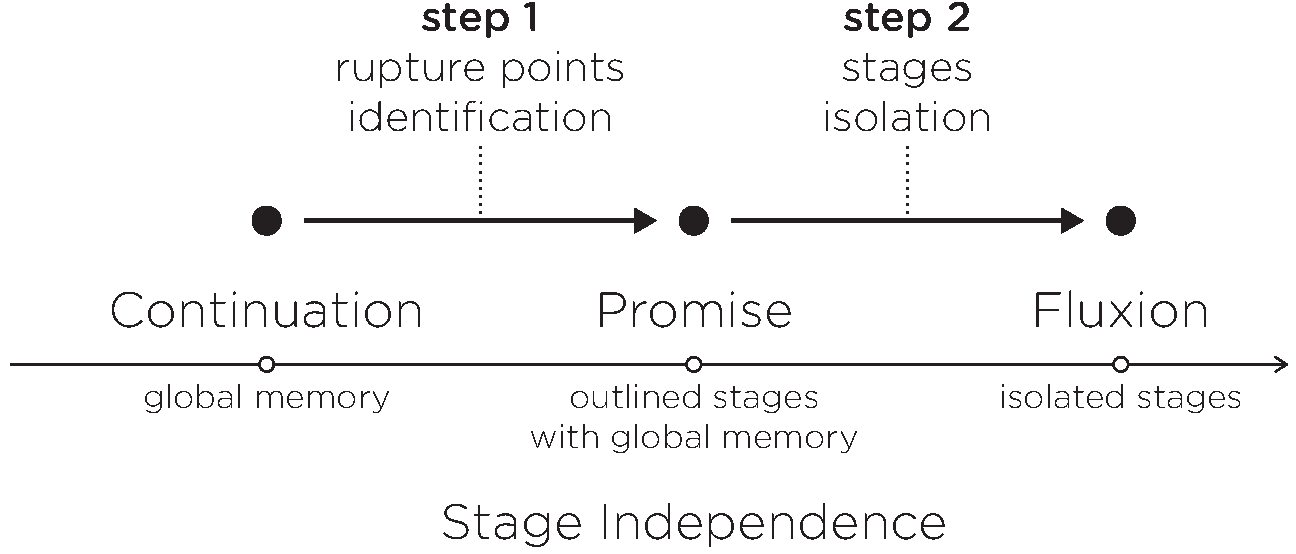
\includegraphics[width=0.7\textwidth]{../resources/roadmap.pdf}%
    \caption{Roadmap}%
    \label{fig:roadmap}%
  }%
\end{figure}

The first compiler focuses on the identification of simple chains of causality between continuations to transform these chains into Promises.
% the transformation from continuations to Promises.
% It focuses on the identification of the chains of causality in continuations.
However, promises are more expressive than the simple chaining of causal sequentiality.
% They force another control over the execution flow.
% According to the outcome of the operation, they call one function to continue the execution with the result, or another to handle errors.
% This conditional execution is indivisible from the Promise specification.
% Promises impose a convention on how to hand back the outcome of the deferred computation, while classic continuations leave this conditional execution to the developer.
Moreover, they impose a different convention than continuations on how to hand back the outcome and errors of the deferred computation.
This difference brings unnecessary complexity to the identification of chains.
To rule out this difference between continuations and Promises, before introducing the first compiler, section \ref{chapter5:due} introduces a simpler specification to Promise, called Due.

The second compiler detects all the chains of causality between continuations and encapsulate them in fluxions.
It isolates the fluxions when possible to allow the parallelism required for efficiency.
This second compilers is introduced in section \ref{chapter5:flx}.

\input{05-implementation/Due/main}
\input{05-implementation/Flx/main}
% \input{05-implementation/Evaluation}

% \subsection{Real test case} \label{chapter5:flx:evaluation}

The compiler is tested on a real application, gifsockets-server\ftnt{https://github.com/twolfson/gifsockets-server}.
This test proves the possibility for an application to be compiled into a network of independent parts.
It shows the current limitations of this isolation and the modifications needed on the application to circumvent them.

\begin{code}[js, caption={Simplified version of gifsockets-server},label={lst:gifsocket}]
var express = require('express'),
    app = express(),
    routes = require('gifsockets-middleware'), //@\label{lst:gifsocket:gif-mw}@
    getRawBody = require('raw-body');

function bodyParser(limit) { //@\label{lst:gifsocket:bodyParser}@
  return function saveBody(req, res, next) { //@\label{lst:gifsocket:saveBody}@
    getRawBody(req, { //@\label{lst:gifsocket:getRawBody}@
      expected: req.headers['content-length'],
      limit: limit
    }, function (err, buffer) { //@\label{lst:gifsocket:callback}@
      req.body = buffer;
      next(); //@\label{lst:gifsocket:next}@
    });
  };
}

app.post('/image/text', bodyParser(1 * 1024 * 1024), routes.writeTextToImages); //@\label{lst:gifsocket:app.post}@
app.listen(8000);
\end{code}

This application, simplified in listing \ref{lst:gifsocket}, is a real-time chat using gif-based communication channels.
It was selected from the evaluation set of the Due compiler because it is simple enough to illustrate this evaluation.
% \cite{Brodu2015}
%  from the \texttt{npm} registry because it depends on \texttt{express}, it is tested, working, and simple enough to illustrate this evaluation.
The server transforms the received text into a gif frame, and pushes it back to a never-ending gif to be displayed on the client.

On line \ref{lst:gifsocket:app.post}, the application registers two functions to process the requests received on the url \texttt{/image/text}.
The closure \texttt{saveBody}, line \ref{lst:gifsocket:saveBody}, returned by \texttt{bodyParser}, line \ref{lst:gifsocket:bodyParser}, and the method \texttt{routes.write\-Text\-To\-Images} from the external module \texttt{gifsockets-\-middleware}, line \ref{lst:gifsocket:gif-mw}.
The closure \texttt{saveBody} calls the asynchronous function \texttt{getRawBody} to get the request body.
Its callback handles the errors, and calls \texttt{next} to continue processing the request with the next function, \texttt{routes.write\-Text\-To\-Images}.

\subsubsection{Compilation} \label{chapter5:flx:evaluation:compilation}

% We compile this application with the compiler
The compilation result is in listing \ref{lst:flx-gifsocket}.
The function call \texttt{app.post}, line \ref{lst:gifsocket:app.post}, is a rupture point.
However, its callbacks, \texttt{bodyParser} and \texttt{routes.write\-Text\-To\-Images} are not declared \textit{in situ}.
They are evaluated as functions only at runtime.
As precised previously, the compiler discards these callbacks to avoid altering the semantic. % by moving or modifying their definition.
% For this reason, the compiler ignores this rupture point, to avoid interfering with the evaluation.

\begin{code}[flx, caption={Compilation result of gifsockets-server},label={lst:flx-gifsocket}]
flx main & express {req}
>> anonymous_1000 [req, next]
  var express = require('express'),
      app = express(),
      routes = require('gifsockets-middleware'), //@\label{lst:flx-gifsocket:gif-mw}@
      getRawBody = require('raw-body');

  function bodyParser(limit) { //@\label{lst:flx-gifsocket:bodyParser}@
    return function saveBody(req, res, next) { //@\label{lst:flx-gifsocket:saveBody}@
      getRawBody(req, { //@\label{lst:flx-gifsocket:getRawBody}@
        expected: req.headers['content-length'], //@\label{lst:flx-gifsocket:req.headers}@
        limit: limit
      }, >> anonymous_1000 [req, next]);
    };
  }

  app.post('/image/text', bodyParser(1 * 1024 * 1024), routes.writeTextToImages); //@\label{lst:flx-gifsocket:app.post}@
  app.listen(8000);

flx anonymous_1000
-> null
  function (err, buffer) { //@\label{lst:flx-gifsocket:callback}@
    req.body = buffer; //@\label{lst:flx-gifsocket:buffer}@
    next(); //@\label{lst:flx-gifsocket:next}@
  }
\end{code}

The compiler detects a rupture point : the function \texttt{get\-Raw\-Body} and its anonymous callback, line \ref{lst:gifsocket:callback}.
It encapsulates this callback in a fluxion named \texttt{anony\-mous\_\-1000}.
The callback is replaced with a stream placeholder to send the message stream to this downstream fluxion.
The variables \texttt{req} and \texttt{next} are appended to this message stream, to propagate their value from the \texttt{main} fluxion to the \texttt{anony\-mous\_\-1000} fluxion.

When \texttt{anony\-mous\_\-1000} is not isolated from the \texttt{main} fluxion, as if they belong to the same group, the compilation result works as expected.
The variables used in the fluxion, \texttt{req} and \texttt{next}, are still shared between the two fluxions.
In this situation fluxions are quite similar to Dues regarding memory shareing.
Our goal is to isolate the two fluxions, to be able to safely parallelize their executions.

\subsubsection{Isolation} \label{chapter5:flx:evaluation:isolation}

In listing \ref{lst:flx-gifsocket}, the fluxion \texttt{anony\-mous\_\-1000} modifies the object \texttt{req}, line \ref{lst:flx-gifsocket:buffer}, to store the text of the received request, and it calls \texttt{next} to continue the execution, line \ref{lst:flx-gifsocket:next}.
\texttt{req} is an alias to a memory location used in multiple palces in code.
Therefore, these operations produce side-effects that should propagate in the whole application, but the isolation prevents this propagation.
Isolating the fluxion \texttt{anony\-mous\_\-1000} produces runtime exceptions.
The next paragraph details how this situation is handled to allow the application to be parallelized.

\paragraph{Variable \texttt{req}}

The variable \texttt{req} is read in fluxion \texttt{main}, lines \ref{lst:flx-gifsocket:getRawBody} and \ref{lst:flx-gifsocket:req.headers}.
Then its property \texttt{body} is associated to \texttt{buffer} in fluxion \texttt{anony\-mous\_\-1000}, line \ref{lst:flx-gifsocket:buffer}.
The compiler is unable to identify the aliases of this variable. % further usages.
However, the side effect resulting from this association impacts a variable in the scope of the next callback, \texttt{routes.write\-Text\-To\-Images}.
In this test case, the application is modified manually to explicitly propagate this side-effect to the next callback through the function \texttt{next}.
The modifications of this function are explained further in the next paragraph.

\paragraph{Closure \texttt{next}}

The function \texttt{next} is a closure provided by the \texttt{express} \texttt{Router} to continue the execution with the next function to handle the client request.
Because it indirectly relies on the variable \texttt{req}, it is impossible to isolate its execution with the \texttt{anony\-mous\_\-1000} fluxion.
Instead, we modify \texttt{express}, so as to be compatible with the fluxional execution model.
We explain the modifications below.

\begin{code}[flx, caption={Simplified modification on the compiled result},label={lst:mflx-gifsocket}]
flx anonymous_1000
-> express_dispatcher
  function (err, buffer) { //@\label{lst:mflx-gifsocket:callback}@
    req.body = buffer; //@\label{lst:mflx-gifsocket:buffer}@
    next_placeholder(req, -> express_dispatcher); //@\label{lst:mflx-gifsocket:next-placeholder}@
  }

flx express_dispatcher & express {req} //@\label{lst:mflx-gifsocket:express-dispatcher}@
-> null
  function (modified_req) {
    merge(req, modified_req);
    next(); //@\label{lst:mflx-gifsocket:next}@
  }
\end{code}

In listing \ref{lst:gifsocket}, the function \texttt{next} is a continuation allowing the anonymous callback, line \ref{lst:gifsocket:callback}, to call the next function to handle the request.
To isolate the anonymous callback into \texttt{anonymous\_\-1000}, \texttt{next} is replaced by a rupture point.
This replacement is illustrated in listing \ref{lst:mflx-gifsocket}.
The \texttt{express} \texttt{Router} registers a fluxion named \texttt{express\_\-dispatcher}, line \ref{lst:mflx-gifsocket:express-dispatcher}, to continue the execution after the fluxion \texttt{anony\-mous\_\-1000}.
This fluxion is in the same group \texttt{express} as the \texttt{main} fluxion, hence it has access to the original variable \texttt{req}, and to the original function \texttt{next}.
The call to the original \texttt{next} function is replaced by a placeholder to push the stream to the fluxion \texttt{express\_\-dispatcher}, line \ref{lst:mflx-gifsocket:next-placeholder}.
The fluxion \texttt{express\_\-dispatcher} receives the stream from the upstream fluxion \texttt{anony\-mous\_\-1000}, merges back the modification in the variable \texttt{req} to propagate the side effects, and finally calls the original function \texttt{next} to continue the execution, line \ref{lst:mflx-gifsocket:next}.

After the modifications detailed above, the server works as expected.
The isolated fluxion correctly receives, and returns its serialized messages.
The client successfully receives a gif frame containing the text.



\subsection{Limitations}

The static analysis used for this compiler presents some limitations.
It is unable to analyze code with dynamic behaviors.
Higher-order programming leads to more productivity partly beacuse it rely on such dynamic behavior to extend expressivity.
Precisely, it allows more levels of indirections.

\subsubsection{Levels of Indirections}

The indirection is an abstraction between the value, and its manipulation.
In listing \ref{lst:indirection}, the variables \texttt{a} and \texttt{b} point both to the same memory object.
The function \texttt{fn} introduces a level of indirection between the real object \texttt{a} and its manipulation handle, \texttt{b};
% Actually, the variable \texttt{a} already introduces a level of indirection between the real object and the handle \texttt{a}.

\begin{code}[js,
  caption={One level of Indirection},
  label={lst:indirection}]
var a = {
      // an object;
    };

fn(b) {
  // modify b;
}

fn(a);
\end{code}

\subsubsection{Uncertainties}

The indirection is trivial to resolve in listing \ref{lst:indirection}.
It only needs to have access to the definition of \texttt{a} and of \texttt{fn}.
%A very simple static analysis could resolve it.
However, in listing \ref{lst:indirections}, the array \texttt{handlers} introduces a new level of indirection.
The static analysis now needs to have access to the definition of \texttt{i} and of the \texttt{handlers}.
If this definition is provided by an external input, it is not available statically, hence, it adds an uncertainty during the analysis. 

\begin{code}[js,
  caption={Two levels of indirection},
  label={lst:indirections}]
var a = {
      // an object;
    },
    handlers = [
      // definition of fn handlers;
    ],
    i = ?;

handlers[i](a);
handlers[i+1](a);
\end{code}

These examples are extremely simplified.
A real application contains enough indirections for the static analysis to be overwhelmed by uncertainties, and to be unable to resolve the variables.
If a variable is left unresolved, it is impossible to assure its scope and its aliases.
Therefore, the compiler is unable to isolate it into a fluxion, or to distribute its modification by messages.

Moreover, it leads the compiler to ignore the rupture points not defined \textit{in situ}, because their modifications could impact the semantic.
The reason for this precaution, is that the compiler is unable to assure where the function is used, and the scope of its variables.
Therefore, it is unable to assure that the modification will conserve the semantic.

\subsubsection{Dynamic Resolution}

In a web application, this variable \texttt{i} might be part of the user request, which is available only at runtime.
It eventually introduces an uncertainty.

This dynamic resolution of variables is precisely what increase expressiveness.
Trying to resolve them statically is equivalent to restrict expressiveness.
No static analysis can overstep these limitations.
Only a dynamic analysis could analysis the resolved indirections during run time to overstep these limitations correctly.




% \subsection{Real test case} \label{chapter5:flx:evaluation}

The compiler is tested on a real application, gifsockets-server\ftnt{https://github.com/twolfson/gifsockets-server}.
This test proves the possibility for an application to be compiled into a network of independent parts.
It shows the current limitations of this isolation and the modifications needed on the application to circumvent them.

\begin{code}[js, caption={Simplified version of gifsockets-server},label={lst:gifsocket}]
var express = require('express'),
    app = express(),
    routes = require('gifsockets-middleware'), //@\label{lst:gifsocket:gif-mw}@
    getRawBody = require('raw-body');

function bodyParser(limit) { //@\label{lst:gifsocket:bodyParser}@
  return function saveBody(req, res, next) { //@\label{lst:gifsocket:saveBody}@
    getRawBody(req, { //@\label{lst:gifsocket:getRawBody}@
      expected: req.headers['content-length'],
      limit: limit
    }, function (err, buffer) { //@\label{lst:gifsocket:callback}@
      req.body = buffer;
      next(); //@\label{lst:gifsocket:next}@
    });
  };
}

app.post('/image/text', bodyParser(1 * 1024 * 1024), routes.writeTextToImages); //@\label{lst:gifsocket:app.post}@
app.listen(8000);
\end{code}

This application, simplified in listing \ref{lst:gifsocket}, is a real-time chat using gif-based communication channels.
It was selected from the evaluation set of the Due compiler because it is simple enough to illustrate this evaluation.
% \cite{Brodu2015}
%  from the \texttt{npm} registry because it depends on \texttt{express}, it is tested, working, and simple enough to illustrate this evaluation.
The server transforms the received text into a gif frame, and pushes it back to a never-ending gif to be displayed on the client.

On line \ref{lst:gifsocket:app.post}, the application registers two functions to process the requests received on the url \texttt{/image/text}.
The closure \texttt{saveBody}, line \ref{lst:gifsocket:saveBody}, returned by \texttt{bodyParser}, line \ref{lst:gifsocket:bodyParser}, and the method \texttt{routes.write\-Text\-To\-Images} from the external module \texttt{gifsockets-\-middleware}, line \ref{lst:gifsocket:gif-mw}.
The closure \texttt{saveBody} calls the asynchronous function \texttt{getRawBody} to get the request body.
Its callback handles the errors, and calls \texttt{next} to continue processing the request with the next function, \texttt{routes.write\-Text\-To\-Images}.

\subsubsection{Compilation} \label{chapter5:flx:evaluation:compilation}

% We compile this application with the compiler
The compilation result is in listing \ref{lst:flx-gifsocket}.
The function call \texttt{app.post}, line \ref{lst:gifsocket:app.post}, is a rupture point.
However, its callbacks, \texttt{bodyParser} and \texttt{routes.write\-Text\-To\-Images} are not declared \textit{in situ}.
They are evaluated as functions only at runtime.
As precised previously, the compiler discards these callbacks to avoid altering the semantic. % by moving or modifying their definition.
% For this reason, the compiler ignores this rupture point, to avoid interfering with the evaluation.

\begin{code}[flx, caption={Compilation result of gifsockets-server},label={lst:flx-gifsocket}]
flx main & express {req}
>> anonymous_1000 [req, next]
  var express = require('express'),
      app = express(),
      routes = require('gifsockets-middleware'), //@\label{lst:flx-gifsocket:gif-mw}@
      getRawBody = require('raw-body');

  function bodyParser(limit) { //@\label{lst:flx-gifsocket:bodyParser}@
    return function saveBody(req, res, next) { //@\label{lst:flx-gifsocket:saveBody}@
      getRawBody(req, { //@\label{lst:flx-gifsocket:getRawBody}@
        expected: req.headers['content-length'], //@\label{lst:flx-gifsocket:req.headers}@
        limit: limit
      }, >> anonymous_1000 [req, next]);
    };
  }

  app.post('/image/text', bodyParser(1 * 1024 * 1024), routes.writeTextToImages); //@\label{lst:flx-gifsocket:app.post}@
  app.listen(8000);

flx anonymous_1000
-> null
  function (err, buffer) { //@\label{lst:flx-gifsocket:callback}@
    req.body = buffer; //@\label{lst:flx-gifsocket:buffer}@
    next(); //@\label{lst:flx-gifsocket:next}@
  }
\end{code}

The compiler detects a rupture point : the function \texttt{get\-Raw\-Body} and its anonymous callback, line \ref{lst:gifsocket:callback}.
It encapsulates this callback in a fluxion named \texttt{anony\-mous\_\-1000}.
The callback is replaced with a stream placeholder to send the message stream to this downstream fluxion.
The variables \texttt{req} and \texttt{next} are appended to this message stream, to propagate their value from the \texttt{main} fluxion to the \texttt{anony\-mous\_\-1000} fluxion.

When \texttt{anony\-mous\_\-1000} is not isolated from the \texttt{main} fluxion, as if they belong to the same group, the compilation result works as expected.
The variables used in the fluxion, \texttt{req} and \texttt{next}, are still shared between the two fluxions.
In this situation fluxions are quite similar to Dues regarding memory shareing.
Our goal is to isolate the two fluxions, to be able to safely parallelize their executions.

\subsubsection{Isolation} \label{chapter5:flx:evaluation:isolation}

In listing \ref{lst:flx-gifsocket}, the fluxion \texttt{anony\-mous\_\-1000} modifies the object \texttt{req}, line \ref{lst:flx-gifsocket:buffer}, to store the text of the received request, and it calls \texttt{next} to continue the execution, line \ref{lst:flx-gifsocket:next}.
\texttt{req} is an alias to a memory location used in multiple palces in code.
Therefore, these operations produce side-effects that should propagate in the whole application, but the isolation prevents this propagation.
Isolating the fluxion \texttt{anony\-mous\_\-1000} produces runtime exceptions.
The next paragraph details how this situation is handled to allow the application to be parallelized.

\paragraph{Variable \texttt{req}}

The variable \texttt{req} is read in fluxion \texttt{main}, lines \ref{lst:flx-gifsocket:getRawBody} and \ref{lst:flx-gifsocket:req.headers}.
Then its property \texttt{body} is associated to \texttt{buffer} in fluxion \texttt{anony\-mous\_\-1000}, line \ref{lst:flx-gifsocket:buffer}.
The compiler is unable to identify the aliases of this variable. % further usages.
However, the side effect resulting from this association impacts a variable in the scope of the next callback, \texttt{routes.write\-Text\-To\-Images}.
In this test case, the application is modified manually to explicitly propagate this side-effect to the next callback through the function \texttt{next}.
The modifications of this function are explained further in the next paragraph.

\paragraph{Closure \texttt{next}}

The function \texttt{next} is a closure provided by the \texttt{express} \texttt{Router} to continue the execution with the next function to handle the client request.
Because it indirectly relies on the variable \texttt{req}, it is impossible to isolate its execution with the \texttt{anony\-mous\_\-1000} fluxion.
Instead, we modify \texttt{express}, so as to be compatible with the fluxional execution model.
We explain the modifications below.

\begin{code}[flx, caption={Simplified modification on the compiled result},label={lst:mflx-gifsocket}]
flx anonymous_1000
-> express_dispatcher
  function (err, buffer) { //@\label{lst:mflx-gifsocket:callback}@
    req.body = buffer; //@\label{lst:mflx-gifsocket:buffer}@
    next_placeholder(req, -> express_dispatcher); //@\label{lst:mflx-gifsocket:next-placeholder}@
  }

flx express_dispatcher & express {req} //@\label{lst:mflx-gifsocket:express-dispatcher}@
-> null
  function (modified_req) {
    merge(req, modified_req);
    next(); //@\label{lst:mflx-gifsocket:next}@
  }
\end{code}

In listing \ref{lst:gifsocket}, the function \texttt{next} is a continuation allowing the anonymous callback, line \ref{lst:gifsocket:callback}, to call the next function to handle the request.
To isolate the anonymous callback into \texttt{anonymous\_\-1000}, \texttt{next} is replaced by a rupture point.
This replacement is illustrated in listing \ref{lst:mflx-gifsocket}.
The \texttt{express} \texttt{Router} registers a fluxion named \texttt{express\_\-dispatcher}, line \ref{lst:mflx-gifsocket:express-dispatcher}, to continue the execution after the fluxion \texttt{anony\-mous\_\-1000}.
This fluxion is in the same group \texttt{express} as the \texttt{main} fluxion, hence it has access to the original variable \texttt{req}, and to the original function \texttt{next}.
The call to the original \texttt{next} function is replaced by a placeholder to push the stream to the fluxion \texttt{express\_\-dispatcher}, line \ref{lst:mflx-gifsocket:next-placeholder}.
The fluxion \texttt{express\_\-dispatcher} receives the stream from the upstream fluxion \texttt{anony\-mous\_\-1000}, merges back the modification in the variable \texttt{req} to propagate the side effects, and finally calls the original function \texttt{next} to continue the execution, line \ref{lst:mflx-gifsocket:next}.

After the modifications detailed above, the server works as expected.
The isolated fluxion correctly receives, and returns its serialized messages.
The client successfully receives a gif frame containing the text.



\subsection{Limitations}

The static analysis used for this compiler presents some limitations.
It is unable to analyze code with dynamic behaviors.
Higher-order programming leads to more productivity partly beacuse it rely on such dynamic behavior to extend expressivity.
Precisely, it allows more levels of indirections.

\subsubsection{Levels of Indirections}

The indirection is an abstraction between the value, and its manipulation.
In listing \ref{lst:indirection}, the variables \texttt{a} and \texttt{b} point both to the same memory object.
The function \texttt{fn} introduces a level of indirection between the real object \texttt{a} and its manipulation handle, \texttt{b};
% Actually, the variable \texttt{a} already introduces a level of indirection between the real object and the handle \texttt{a}.

\begin{code}[js,
  caption={One level of Indirection},
  label={lst:indirection}]
var a = {
      // an object;
    };

fn(b) {
  // modify b;
}

fn(a);
\end{code}

\subsubsection{Uncertainties}

The indirection is trivial to resolve in listing \ref{lst:indirection}.
It only needs to have access to the definition of \texttt{a} and of \texttt{fn}.
%A very simple static analysis could resolve it.
However, in listing \ref{lst:indirections}, the array \texttt{handlers} introduces a new level of indirection.
The static analysis now needs to have access to the definition of \texttt{i} and of the \texttt{handlers}.
If this definition is provided by an external input, it is not available statically, hence, it adds an uncertainty during the analysis. 

\begin{code}[js,
  caption={Two levels of indirection},
  label={lst:indirections}]
var a = {
      // an object;
    },
    handlers = [
      // definition of fn handlers;
    ],
    i = ?;

handlers[i](a);
handlers[i+1](a);
\end{code}

These examples are extremely simplified.
A real application contains enough indirections for the static analysis to be overwhelmed by uncertainties, and to be unable to resolve the variables.
If a variable is left unresolved, it is impossible to assure its scope and its aliases.
Therefore, the compiler is unable to isolate it into a fluxion, or to distribute its modification by messages.

Moreover, it leads the compiler to ignore the rupture points not defined \textit{in situ}, because their modifications could impact the semantic.
The reason for this precaution, is that the compiler is unable to assure where the function is used, and the scope of its variables.
Therefore, it is unable to assure that the modification will conserve the semantic.

\subsubsection{Dynamic Resolution}

In a web application, this variable \texttt{i} might be part of the user request, which is available only at runtime.
It eventually introduces an uncertainty.

This dynamic resolution of variables is precisely what increase expressiveness.
Trying to resolve them statically is equivalent to restrict expressiveness.
No static analysis can overstep these limitations.
Only a dynamic analysis could analysis the resolved indirections during run time to overstep these limitations correctly.





% iconfont\\
% \foreach \x in {0,...,646}
%    {\x\thinspace\iconfont{\XeTeXglyph\x} }\\
% typicons\\
% \foreach \x in {0,...,336}
%    {\x\thinspace\typicons{\XeTeXglyph\x} }\\
% elusive\\
% \foreach \x in {0,...,300}
%    {\x\thinspace\elusive{\XeTeXglyph\x} }\\
% linecons\\
% \foreach \x in {0,...,50}
%    {\x\thinspace\linecons{\XeTeXglyph\x} }\\
% \eject


\topskip0pt
\vspace*{\fill}
\section*{Acknowledgments}
\begin{flushleft}
\noindent%
\textit{
~\\
I would like to expressly thank\\
Stéphane Frénot, Frédéric Oblé, and Fabien Cellier who had the patience to tutor me during the last three years despite my stubbornness and clumsiness.
% It must have been at least three times as painfull for them as it was for me.
\\[30pt]
%
I would like to kindly thank my parents and family.\\
Hadn't you trusted me to dismantle stuffs and fix computers,\\
I would never have followed this path.\\
{\elusive{\XeTeXglyph166}}\\[30pt]
%
A huge thank to my coworkers, at Worldline and Dice.\\
We shared some office spaces, but more than that, some memorable pieces of fun together.\\
{\iconfont{\XeTeXglyph580}}\\[30pt]
%
A huge thank to my friends who supported me, and are still talking to me even if I was available to hang out barely one hour a week.\\
{\iconfont{\XeTeXglyph582}}\\[30pt]
%
% A special thank to Boris Vacher.\\
% The spark you expected never came. I am still actively looking for it, but I am doubting it will ever come.\\
% {\iconfont{\XeTeXglyph279}}\\[30pt]
%
Thanks to you that is reading this.\\
I hope this work will prove worthy of your time.
\\[30pt]
%
And finally, I would like to thank matter, time, and all the physical constants to be what they are.
Without you, nothing could be.
}
\end{flushleft}
\noindent {\huge Thanks to all of you.}\\
\vspace*{\fill}
\eject

% \dominitoc%
% \etocsettocstyle{Content}{}%

% \renewcommand{\cfttoctitlefont}{\normalfont\Large\bfseries\MakeUppercase}
% \renewcommand{\contentsname}{Contents}
% \renewcommand{\cftchapfont}{\secfont\fontsize{17pt}{17pt}\selectfont\MakeUppercase}
% \renewcommand{\cftchapfont}{\secfont\fontsize{20pt}{20pt}\selectfont}

\tableofcontents\newpage%\eject
\listoffigures\newpage%\eject
\listoftables\newpage%\eject
\listofillustration%

\etocsettocstyle{}{}%
\cftsecindent 0pt
% \cftsubsecindent 25pt
\pagestyle{fancy}

\renewcommand{\glyph}{\iconfont{\XeTeXglyph287}}
\chapter{Implementations} \label{chapter5}
\minitoc
\eject
The transformation allowed by the equivalence from an event-driven program into a distributed network of fluxions is implemented incrementally into two compilers, as presented in figure \ref{fig:roadmap}.
Each compilers is divided into two steps, the identification of the rupture points separating the stages of the pipeline, and the isolation of these stages.
% This chapter presents the technical implementations of these two steps in the transformation from the event-driven execution model to the pipeline architecture
% , the transformation described in the previous chapter was implemented incrementally in two compilers.

\begin{figure}[h!]%
  \textfig{%
    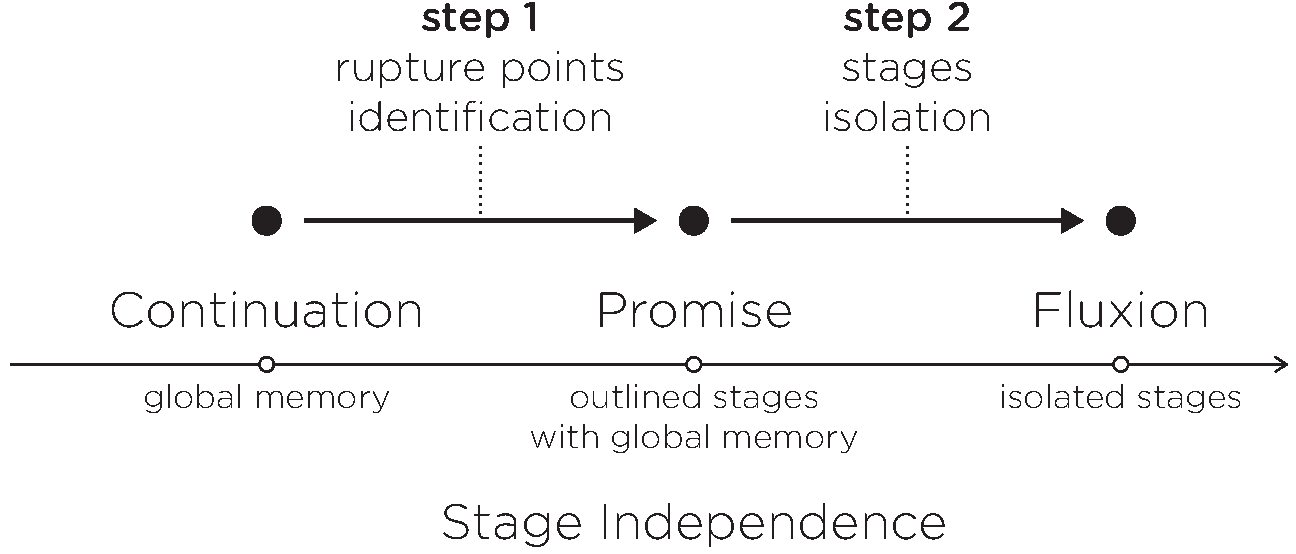
\includegraphics[width=0.7\textwidth]{../resources/roadmap.pdf}%
    \caption{Roadmap}%
    \label{fig:roadmap}%
  }%
\end{figure}

The first compiler focuses on the identification of simple chains of causality between continuations to transform these chains into Promises.
% the transformation from continuations to Promises.
% It focuses on the identification of the chains of causality in continuations.
However, promises are more expressive than the simple chaining of causal sequentiality.
% They force another control over the execution flow.
% According to the outcome of the operation, they call one function to continue the execution with the result, or another to handle errors.
% This conditional execution is indivisible from the Promise specification.
% Promises impose a convention on how to hand back the outcome of the deferred computation, while classic continuations leave this conditional execution to the developer.
Moreover, they impose a different convention than continuations on how to hand back the outcome and errors of the deferred computation.
This difference brings unnecessary complexity to the identification of chains.
To rule out this difference between continuations and Promises, before introducing the first compiler, section \ref{chapter5:due} introduces a simpler specification to Promise, called Due.

The second compiler detects all the chains of causality between continuations and encapsulate them in fluxions.
It isolates the fluxions when possible to allow the parallelism required for efficiency.
This second compilers is introduced in section \ref{chapter5:flx}.

\renewcommand{\glyph}{\iconfont{\XeTeXglyph287}}
\chapter{Implementations} \label{chapter5}
\minitoc
\eject
The transformation allowed by the equivalence from an event-driven program into a distributed network of fluxions is implemented incrementally into two compilers, as presented in figure \ref{fig:roadmap}.
Each compilers is divided into two steps, the identification of the rupture points separating the stages of the pipeline, and the isolation of these stages.
% This chapter presents the technical implementations of these two steps in the transformation from the event-driven execution model to the pipeline architecture
% , the transformation described in the previous chapter was implemented incrementally in two compilers.

\begin{figure}[h!]%
  \textfig{%
    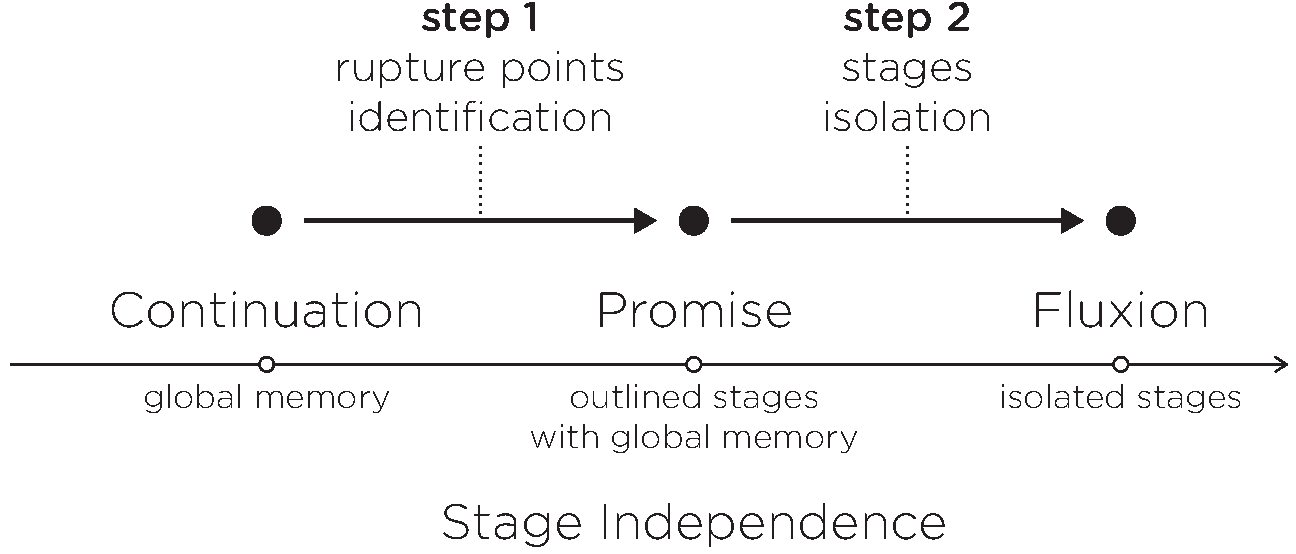
\includegraphics[width=0.7\textwidth]{../resources/roadmap.pdf}%
    \caption{Roadmap}%
    \label{fig:roadmap}%
  }%
\end{figure}

The first compiler focuses on the identification of simple chains of causality between continuations to transform these chains into Promises.
% the transformation from continuations to Promises.
% It focuses on the identification of the chains of causality in continuations.
However, promises are more expressive than the simple chaining of causal sequentiality.
% They force another control over the execution flow.
% According to the outcome of the operation, they call one function to continue the execution with the result, or another to handle errors.
% This conditional execution is indivisible from the Promise specification.
% Promises impose a convention on how to hand back the outcome of the deferred computation, while classic continuations leave this conditional execution to the developer.
Moreover, they impose a different convention than continuations on how to hand back the outcome and errors of the deferred computation.
This difference brings unnecessary complexity to the identification of chains.
To rule out this difference between continuations and Promises, before introducing the first compiler, section \ref{chapter5:due} introduces a simpler specification to Promise, called Due.

The second compiler detects all the chains of causality between continuations and encapsulate them in fluxions.
It isolates the fluxions when possible to allow the parallelism required for efficiency.
This second compilers is introduced in section \ref{chapter5:flx}.

\renewcommand{\glyph}{\iconfont{\XeTeXglyph287}}
\chapter{Implementations} \label{chapter5}
\minitoc
\eject
The transformation allowed by the equivalence from an event-driven program into a distributed network of fluxions is implemented incrementally into two compilers, as presented in figure \ref{fig:roadmap}.
Each compilers is divided into two steps, the identification of the rupture points separating the stages of the pipeline, and the isolation of these stages.
% This chapter presents the technical implementations of these two steps in the transformation from the event-driven execution model to the pipeline architecture
% , the transformation described in the previous chapter was implemented incrementally in two compilers.

\begin{figure}[h!]%
  \textfig{%
    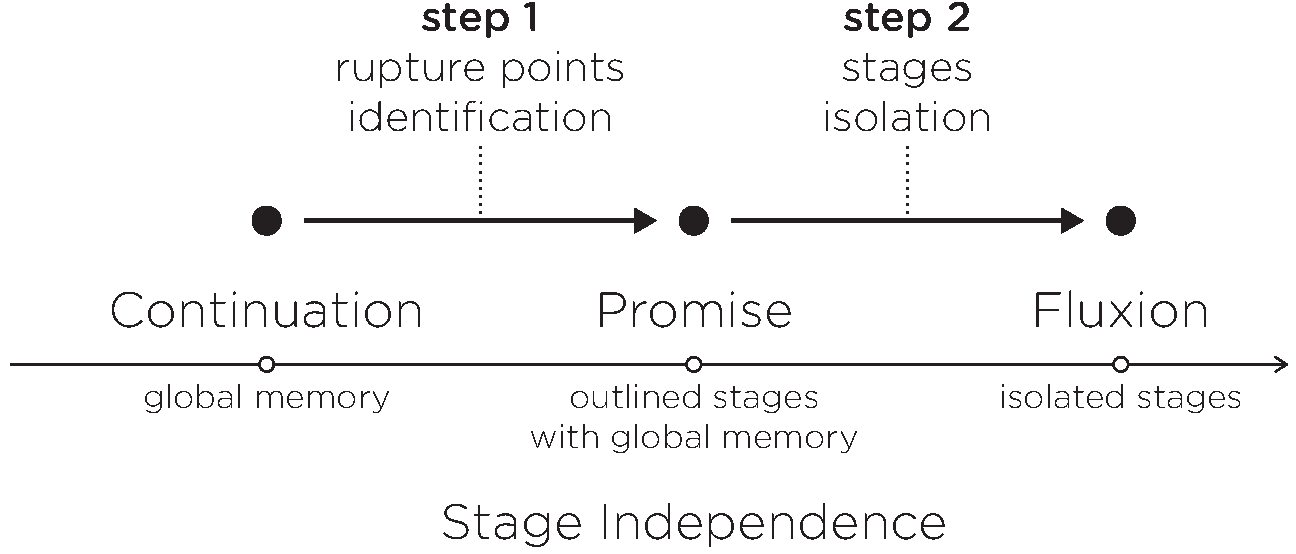
\includegraphics[width=0.7\textwidth]{../resources/roadmap.pdf}%
    \caption{Roadmap}%
    \label{fig:roadmap}%
  }%
\end{figure}

The first compiler focuses on the identification of simple chains of causality between continuations to transform these chains into Promises.
% the transformation from continuations to Promises.
% It focuses on the identification of the chains of causality in continuations.
However, promises are more expressive than the simple chaining of causal sequentiality.
% They force another control over the execution flow.
% According to the outcome of the operation, they call one function to continue the execution with the result, or another to handle errors.
% This conditional execution is indivisible from the Promise specification.
% Promises impose a convention on how to hand back the outcome of the deferred computation, while classic continuations leave this conditional execution to the developer.
Moreover, they impose a different convention than continuations on how to hand back the outcome and errors of the deferred computation.
This difference brings unnecessary complexity to the identification of chains.
To rule out this difference between continuations and Promises, before introducing the first compiler, section \ref{chapter5:due} introduces a simpler specification to Promise, called Due.

The second compiler detects all the chains of causality between continuations and encapsulate them in fluxions.
It isolates the fluxions when possible to allow the parallelism required for efficiency.
This second compilers is introduced in section \ref{chapter5:flx}.

\input{05-implementation/Due/main}
\input{05-implementation/Flx/main}
% \input{05-implementation/Evaluation}

\renewcommand{\glyph}{\iconfont{\XeTeXglyph287}}
\chapter{Implementations} \label{chapter5}
\minitoc
\eject
The transformation allowed by the equivalence from an event-driven program into a distributed network of fluxions is implemented incrementally into two compilers, as presented in figure \ref{fig:roadmap}.
Each compilers is divided into two steps, the identification of the rupture points separating the stages of the pipeline, and the isolation of these stages.
% This chapter presents the technical implementations of these two steps in the transformation from the event-driven execution model to the pipeline architecture
% , the transformation described in the previous chapter was implemented incrementally in two compilers.

\begin{figure}[h!]%
  \textfig{%
    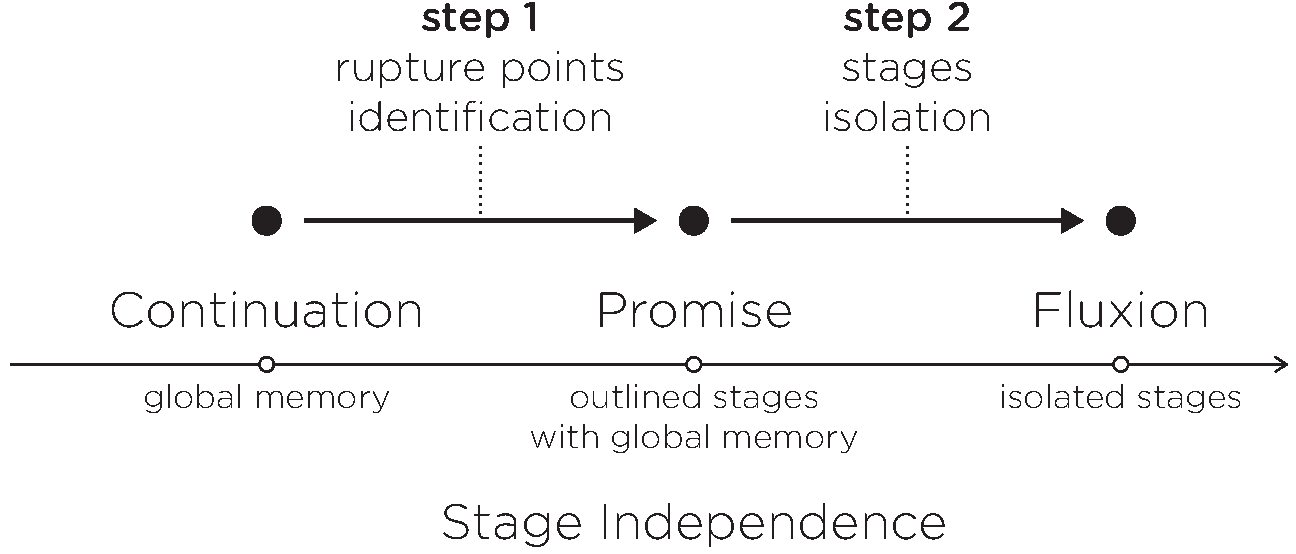
\includegraphics[width=0.7\textwidth]{../resources/roadmap.pdf}%
    \caption{Roadmap}%
    \label{fig:roadmap}%
  }%
\end{figure}

The first compiler focuses on the identification of simple chains of causality between continuations to transform these chains into Promises.
% the transformation from continuations to Promises.
% It focuses on the identification of the chains of causality in continuations.
However, promises are more expressive than the simple chaining of causal sequentiality.
% They force another control over the execution flow.
% According to the outcome of the operation, they call one function to continue the execution with the result, or another to handle errors.
% This conditional execution is indivisible from the Promise specification.
% Promises impose a convention on how to hand back the outcome of the deferred computation, while classic continuations leave this conditional execution to the developer.
Moreover, they impose a different convention than continuations on how to hand back the outcome and errors of the deferred computation.
This difference brings unnecessary complexity to the identification of chains.
To rule out this difference between continuations and Promises, before introducing the first compiler, section \ref{chapter5:due} introduces a simpler specification to Promise, called Due.

The second compiler detects all the chains of causality between continuations and encapsulate them in fluxions.
It isolates the fluxions when possible to allow the parallelism required for efficiency.
This second compilers is introduced in section \ref{chapter5:flx}.

\input{05-implementation/Due/main}
\input{05-implementation/Flx/main}
% \input{05-implementation/Evaluation}

% \subsection{Real test case} \label{chapter5:flx:evaluation}

The compiler is tested on a real application, gifsockets-server\ftnt{https://github.com/twolfson/gifsockets-server}.
This test proves the possibility for an application to be compiled into a network of independent parts.
It shows the current limitations of this isolation and the modifications needed on the application to circumvent them.

\begin{code}[js, caption={Simplified version of gifsockets-server},label={lst:gifsocket}]
var express = require('express'),
    app = express(),
    routes = require('gifsockets-middleware'), //@\label{lst:gifsocket:gif-mw}@
    getRawBody = require('raw-body');

function bodyParser(limit) { //@\label{lst:gifsocket:bodyParser}@
  return function saveBody(req, res, next) { //@\label{lst:gifsocket:saveBody}@
    getRawBody(req, { //@\label{lst:gifsocket:getRawBody}@
      expected: req.headers['content-length'],
      limit: limit
    }, function (err, buffer) { //@\label{lst:gifsocket:callback}@
      req.body = buffer;
      next(); //@\label{lst:gifsocket:next}@
    });
  };
}

app.post('/image/text', bodyParser(1 * 1024 * 1024), routes.writeTextToImages); //@\label{lst:gifsocket:app.post}@
app.listen(8000);
\end{code}

This application, simplified in listing \ref{lst:gifsocket}, is a real-time chat using gif-based communication channels.
It was selected from the evaluation set of the Due compiler because it is simple enough to illustrate this evaluation.
% \cite{Brodu2015}
%  from the \texttt{npm} registry because it depends on \texttt{express}, it is tested, working, and simple enough to illustrate this evaluation.
The server transforms the received text into a gif frame, and pushes it back to a never-ending gif to be displayed on the client.

On line \ref{lst:gifsocket:app.post}, the application registers two functions to process the requests received on the url \texttt{/image/text}.
The closure \texttt{saveBody}, line \ref{lst:gifsocket:saveBody}, returned by \texttt{bodyParser}, line \ref{lst:gifsocket:bodyParser}, and the method \texttt{routes.write\-Text\-To\-Images} from the external module \texttt{gifsockets-\-middleware}, line \ref{lst:gifsocket:gif-mw}.
The closure \texttt{saveBody} calls the asynchronous function \texttt{getRawBody} to get the request body.
Its callback handles the errors, and calls \texttt{next} to continue processing the request with the next function, \texttt{routes.write\-Text\-To\-Images}.

\subsubsection{Compilation} \label{chapter5:flx:evaluation:compilation}

% We compile this application with the compiler
The compilation result is in listing \ref{lst:flx-gifsocket}.
The function call \texttt{app.post}, line \ref{lst:gifsocket:app.post}, is a rupture point.
However, its callbacks, \texttt{bodyParser} and \texttt{routes.write\-Text\-To\-Images} are not declared \textit{in situ}.
They are evaluated as functions only at runtime.
As precised previously, the compiler discards these callbacks to avoid altering the semantic. % by moving or modifying their definition.
% For this reason, the compiler ignores this rupture point, to avoid interfering with the evaluation.

\begin{code}[flx, caption={Compilation result of gifsockets-server},label={lst:flx-gifsocket}]
flx main & express {req}
>> anonymous_1000 [req, next]
  var express = require('express'),
      app = express(),
      routes = require('gifsockets-middleware'), //@\label{lst:flx-gifsocket:gif-mw}@
      getRawBody = require('raw-body');

  function bodyParser(limit) { //@\label{lst:flx-gifsocket:bodyParser}@
    return function saveBody(req, res, next) { //@\label{lst:flx-gifsocket:saveBody}@
      getRawBody(req, { //@\label{lst:flx-gifsocket:getRawBody}@
        expected: req.headers['content-length'], //@\label{lst:flx-gifsocket:req.headers}@
        limit: limit
      }, >> anonymous_1000 [req, next]);
    };
  }

  app.post('/image/text', bodyParser(1 * 1024 * 1024), routes.writeTextToImages); //@\label{lst:flx-gifsocket:app.post}@
  app.listen(8000);

flx anonymous_1000
-> null
  function (err, buffer) { //@\label{lst:flx-gifsocket:callback}@
    req.body = buffer; //@\label{lst:flx-gifsocket:buffer}@
    next(); //@\label{lst:flx-gifsocket:next}@
  }
\end{code}

The compiler detects a rupture point : the function \texttt{get\-Raw\-Body} and its anonymous callback, line \ref{lst:gifsocket:callback}.
It encapsulates this callback in a fluxion named \texttt{anony\-mous\_\-1000}.
The callback is replaced with a stream placeholder to send the message stream to this downstream fluxion.
The variables \texttt{req} and \texttt{next} are appended to this message stream, to propagate their value from the \texttt{main} fluxion to the \texttt{anony\-mous\_\-1000} fluxion.

When \texttt{anony\-mous\_\-1000} is not isolated from the \texttt{main} fluxion, as if they belong to the same group, the compilation result works as expected.
The variables used in the fluxion, \texttt{req} and \texttt{next}, are still shared between the two fluxions.
In this situation fluxions are quite similar to Dues regarding memory shareing.
Our goal is to isolate the two fluxions, to be able to safely parallelize their executions.

\subsubsection{Isolation} \label{chapter5:flx:evaluation:isolation}

In listing \ref{lst:flx-gifsocket}, the fluxion \texttt{anony\-mous\_\-1000} modifies the object \texttt{req}, line \ref{lst:flx-gifsocket:buffer}, to store the text of the received request, and it calls \texttt{next} to continue the execution, line \ref{lst:flx-gifsocket:next}.
\texttt{req} is an alias to a memory location used in multiple palces in code.
Therefore, these operations produce side-effects that should propagate in the whole application, but the isolation prevents this propagation.
Isolating the fluxion \texttt{anony\-mous\_\-1000} produces runtime exceptions.
The next paragraph details how this situation is handled to allow the application to be parallelized.

\paragraph{Variable \texttt{req}}

The variable \texttt{req} is read in fluxion \texttt{main}, lines \ref{lst:flx-gifsocket:getRawBody} and \ref{lst:flx-gifsocket:req.headers}.
Then its property \texttt{body} is associated to \texttt{buffer} in fluxion \texttt{anony\-mous\_\-1000}, line \ref{lst:flx-gifsocket:buffer}.
The compiler is unable to identify the aliases of this variable. % further usages.
However, the side effect resulting from this association impacts a variable in the scope of the next callback, \texttt{routes.write\-Text\-To\-Images}.
In this test case, the application is modified manually to explicitly propagate this side-effect to the next callback through the function \texttt{next}.
The modifications of this function are explained further in the next paragraph.

\paragraph{Closure \texttt{next}}

The function \texttt{next} is a closure provided by the \texttt{express} \texttt{Router} to continue the execution with the next function to handle the client request.
Because it indirectly relies on the variable \texttt{req}, it is impossible to isolate its execution with the \texttt{anony\-mous\_\-1000} fluxion.
Instead, we modify \texttt{express}, so as to be compatible with the fluxional execution model.
We explain the modifications below.

\begin{code}[flx, caption={Simplified modification on the compiled result},label={lst:mflx-gifsocket}]
flx anonymous_1000
-> express_dispatcher
  function (err, buffer) { //@\label{lst:mflx-gifsocket:callback}@
    req.body = buffer; //@\label{lst:mflx-gifsocket:buffer}@
    next_placeholder(req, -> express_dispatcher); //@\label{lst:mflx-gifsocket:next-placeholder}@
  }

flx express_dispatcher & express {req} //@\label{lst:mflx-gifsocket:express-dispatcher}@
-> null
  function (modified_req) {
    merge(req, modified_req);
    next(); //@\label{lst:mflx-gifsocket:next}@
  }
\end{code}

In listing \ref{lst:gifsocket}, the function \texttt{next} is a continuation allowing the anonymous callback, line \ref{lst:gifsocket:callback}, to call the next function to handle the request.
To isolate the anonymous callback into \texttt{anonymous\_\-1000}, \texttt{next} is replaced by a rupture point.
This replacement is illustrated in listing \ref{lst:mflx-gifsocket}.
The \texttt{express} \texttt{Router} registers a fluxion named \texttt{express\_\-dispatcher}, line \ref{lst:mflx-gifsocket:express-dispatcher}, to continue the execution after the fluxion \texttt{anony\-mous\_\-1000}.
This fluxion is in the same group \texttt{express} as the \texttt{main} fluxion, hence it has access to the original variable \texttt{req}, and to the original function \texttt{next}.
The call to the original \texttt{next} function is replaced by a placeholder to push the stream to the fluxion \texttt{express\_\-dispatcher}, line \ref{lst:mflx-gifsocket:next-placeholder}.
The fluxion \texttt{express\_\-dispatcher} receives the stream from the upstream fluxion \texttt{anony\-mous\_\-1000}, merges back the modification in the variable \texttt{req} to propagate the side effects, and finally calls the original function \texttt{next} to continue the execution, line \ref{lst:mflx-gifsocket:next}.

After the modifications detailed above, the server works as expected.
The isolated fluxion correctly receives, and returns its serialized messages.
The client successfully receives a gif frame containing the text.



\subsection{Limitations}

The static analysis used for this compiler presents some limitations.
It is unable to analyze code with dynamic behaviors.
Higher-order programming leads to more productivity partly beacuse it rely on such dynamic behavior to extend expressivity.
Precisely, it allows more levels of indirections.

\subsubsection{Levels of Indirections}

The indirection is an abstraction between the value, and its manipulation.
In listing \ref{lst:indirection}, the variables \texttt{a} and \texttt{b} point both to the same memory object.
The function \texttt{fn} introduces a level of indirection between the real object \texttt{a} and its manipulation handle, \texttt{b};
% Actually, the variable \texttt{a} already introduces a level of indirection between the real object and the handle \texttt{a}.

\begin{code}[js,
  caption={One level of Indirection},
  label={lst:indirection}]
var a = {
      // an object;
    };

fn(b) {
  // modify b;
}

fn(a);
\end{code}

\subsubsection{Uncertainties}

The indirection is trivial to resolve in listing \ref{lst:indirection}.
It only needs to have access to the definition of \texttt{a} and of \texttt{fn}.
%A very simple static analysis could resolve it.
However, in listing \ref{lst:indirections}, the array \texttt{handlers} introduces a new level of indirection.
The static analysis now needs to have access to the definition of \texttt{i} and of the \texttt{handlers}.
If this definition is provided by an external input, it is not available statically, hence, it adds an uncertainty during the analysis. 

\begin{code}[js,
  caption={Two levels of indirection},
  label={lst:indirections}]
var a = {
      // an object;
    },
    handlers = [
      // definition of fn handlers;
    ],
    i = ?;

handlers[i](a);
handlers[i+1](a);
\end{code}

These examples are extremely simplified.
A real application contains enough indirections for the static analysis to be overwhelmed by uncertainties, and to be unable to resolve the variables.
If a variable is left unresolved, it is impossible to assure its scope and its aliases.
Therefore, the compiler is unable to isolate it into a fluxion, or to distribute its modification by messages.

Moreover, it leads the compiler to ignore the rupture points not defined \textit{in situ}, because their modifications could impact the semantic.
The reason for this precaution, is that the compiler is unable to assure where the function is used, and the scope of its variables.
Therefore, it is unable to assure that the modification will conserve the semantic.

\subsubsection{Dynamic Resolution}

In a web application, this variable \texttt{i} might be part of the user request, which is available only at runtime.
It eventually introduces an uncertainty.

This dynamic resolution of variables is precisely what increase expressiveness.
Trying to resolve them statically is equivalent to restrict expressiveness.
No static analysis can overstep these limitations.
Only a dynamic analysis could analysis the resolved indirections during run time to overstep these limitations correctly.




\renewcommand{\glyph}{\iconfont{\XeTeXglyph287}}
\chapter{Implementations} \label{chapter5}
\minitoc
\eject
The transformation allowed by the equivalence from an event-driven program into a distributed network of fluxions is implemented incrementally into two compilers, as presented in figure \ref{fig:roadmap}.
Each compilers is divided into two steps, the identification of the rupture points separating the stages of the pipeline, and the isolation of these stages.
% This chapter presents the technical implementations of these two steps in the transformation from the event-driven execution model to the pipeline architecture
% , the transformation described in the previous chapter was implemented incrementally in two compilers.

\begin{figure}[h!]%
  \textfig{%
    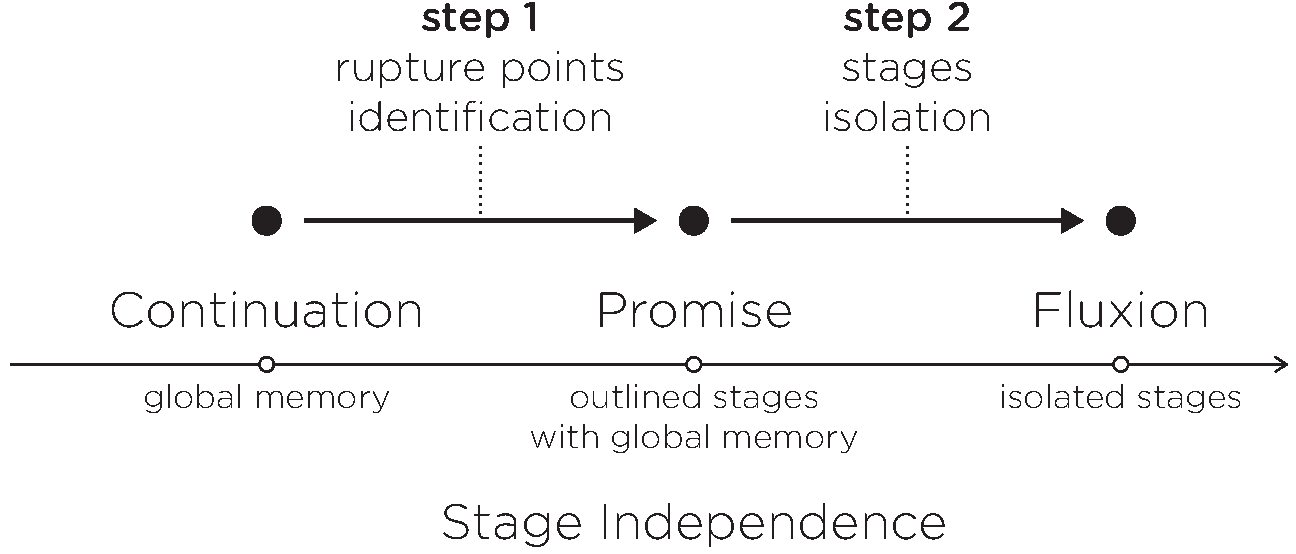
\includegraphics[width=0.7\textwidth]{../resources/roadmap.pdf}%
    \caption{Roadmap}%
    \label{fig:roadmap}%
  }%
\end{figure}

The first compiler focuses on the identification of simple chains of causality between continuations to transform these chains into Promises.
% the transformation from continuations to Promises.
% It focuses on the identification of the chains of causality in continuations.
However, promises are more expressive than the simple chaining of causal sequentiality.
% They force another control over the execution flow.
% According to the outcome of the operation, they call one function to continue the execution with the result, or another to handle errors.
% This conditional execution is indivisible from the Promise specification.
% Promises impose a convention on how to hand back the outcome of the deferred computation, while classic continuations leave this conditional execution to the developer.
Moreover, they impose a different convention than continuations on how to hand back the outcome and errors of the deferred computation.
This difference brings unnecessary complexity to the identification of chains.
To rule out this difference between continuations and Promises, before introducing the first compiler, section \ref{chapter5:due} introduces a simpler specification to Promise, called Due.

The second compiler detects all the chains of causality between continuations and encapsulate them in fluxions.
It isolates the fluxions when possible to allow the parallelism required for efficiency.
This second compilers is introduced in section \ref{chapter5:flx}.

\renewcommand{\glyph}{\iconfont{\XeTeXglyph287}}
\chapter{Implementations} \label{chapter5}
\minitoc
\eject
The transformation allowed by the equivalence from an event-driven program into a distributed network of fluxions is implemented incrementally into two compilers, as presented in figure \ref{fig:roadmap}.
Each compilers is divided into two steps, the identification of the rupture points separating the stages of the pipeline, and the isolation of these stages.
% This chapter presents the technical implementations of these two steps in the transformation from the event-driven execution model to the pipeline architecture
% , the transformation described in the previous chapter was implemented incrementally in two compilers.

\begin{figure}[h!]%
  \textfig{%
    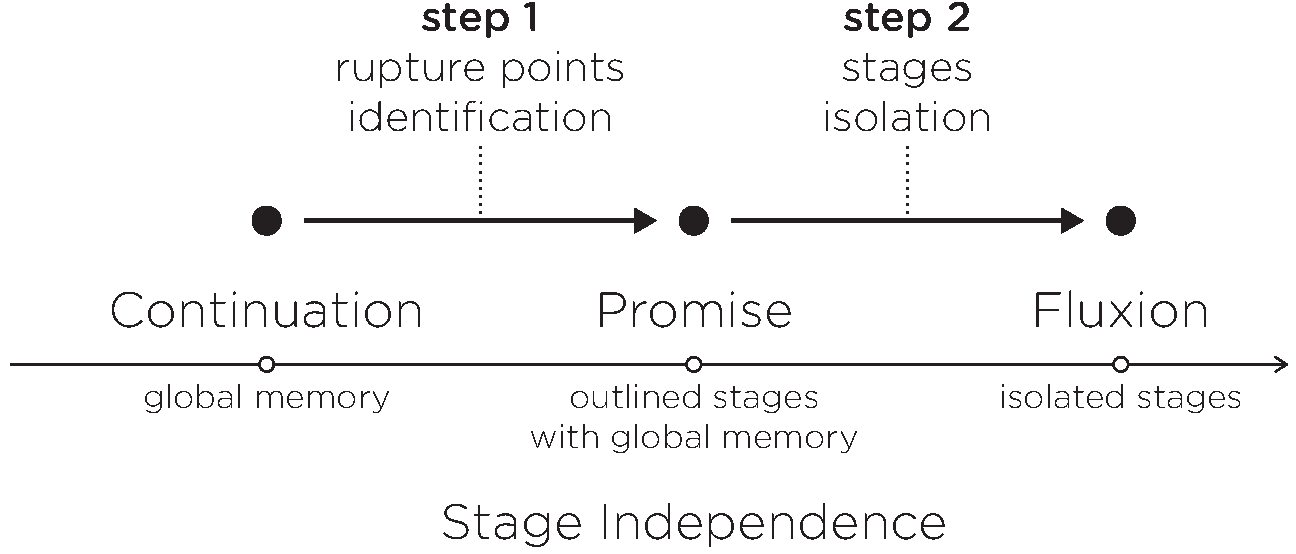
\includegraphics[width=0.7\textwidth]{../resources/roadmap.pdf}%
    \caption{Roadmap}%
    \label{fig:roadmap}%
  }%
\end{figure}

The first compiler focuses on the identification of simple chains of causality between continuations to transform these chains into Promises.
% the transformation from continuations to Promises.
% It focuses on the identification of the chains of causality in continuations.
However, promises are more expressive than the simple chaining of causal sequentiality.
% They force another control over the execution flow.
% According to the outcome of the operation, they call one function to continue the execution with the result, or another to handle errors.
% This conditional execution is indivisible from the Promise specification.
% Promises impose a convention on how to hand back the outcome of the deferred computation, while classic continuations leave this conditional execution to the developer.
Moreover, they impose a different convention than continuations on how to hand back the outcome and errors of the deferred computation.
This difference brings unnecessary complexity to the identification of chains.
To rule out this difference between continuations and Promises, before introducing the first compiler, section \ref{chapter5:due} introduces a simpler specification to Promise, called Due.

The second compiler detects all the chains of causality between continuations and encapsulate them in fluxions.
It isolates the fluxions when possible to allow the parallelism required for efficiency.
This second compilers is introduced in section \ref{chapter5:flx}.

\input{05-implementation/Due/main}
\input{05-implementation/Flx/main}
% \input{05-implementation/Evaluation}

\renewcommand{\glyph}{\iconfont{\XeTeXglyph287}}
\chapter{Implementations} \label{chapter5}
\minitoc
\eject
The transformation allowed by the equivalence from an event-driven program into a distributed network of fluxions is implemented incrementally into two compilers, as presented in figure \ref{fig:roadmap}.
Each compilers is divided into two steps, the identification of the rupture points separating the stages of the pipeline, and the isolation of these stages.
% This chapter presents the technical implementations of these two steps in the transformation from the event-driven execution model to the pipeline architecture
% , the transformation described in the previous chapter was implemented incrementally in two compilers.

\begin{figure}[h!]%
  \textfig{%
    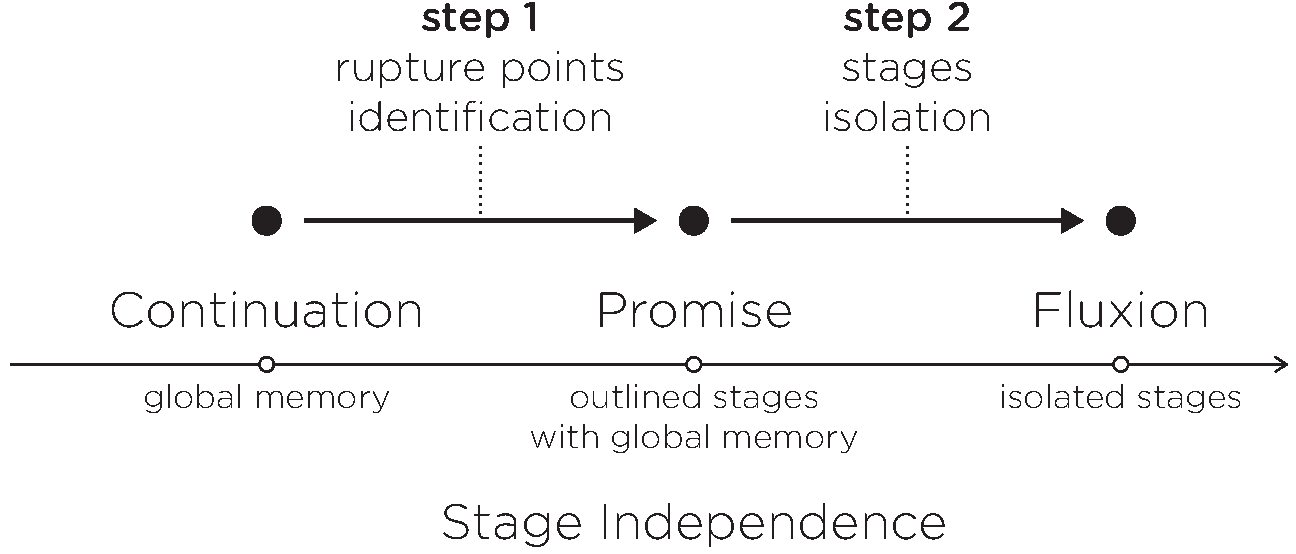
\includegraphics[width=0.7\textwidth]{../resources/roadmap.pdf}%
    \caption{Roadmap}%
    \label{fig:roadmap}%
  }%
\end{figure}

The first compiler focuses on the identification of simple chains of causality between continuations to transform these chains into Promises.
% the transformation from continuations to Promises.
% It focuses on the identification of the chains of causality in continuations.
However, promises are more expressive than the simple chaining of causal sequentiality.
% They force another control over the execution flow.
% According to the outcome of the operation, they call one function to continue the execution with the result, or another to handle errors.
% This conditional execution is indivisible from the Promise specification.
% Promises impose a convention on how to hand back the outcome of the deferred computation, while classic continuations leave this conditional execution to the developer.
Moreover, they impose a different convention than continuations on how to hand back the outcome and errors of the deferred computation.
This difference brings unnecessary complexity to the identification of chains.
To rule out this difference between continuations and Promises, before introducing the first compiler, section \ref{chapter5:due} introduces a simpler specification to Promise, called Due.

The second compiler detects all the chains of causality between continuations and encapsulate them in fluxions.
It isolates the fluxions when possible to allow the parallelism required for efficiency.
This second compilers is introduced in section \ref{chapter5:flx}.

\input{05-implementation/Due/main}
\input{05-implementation/Flx/main}
% \input{05-implementation/Evaluation}

% \subsection{Real test case} \label{chapter5:flx:evaluation}

The compiler is tested on a real application, gifsockets-server\ftnt{https://github.com/twolfson/gifsockets-server}.
This test proves the possibility for an application to be compiled into a network of independent parts.
It shows the current limitations of this isolation and the modifications needed on the application to circumvent them.

\begin{code}[js, caption={Simplified version of gifsockets-server},label={lst:gifsocket}]
var express = require('express'),
    app = express(),
    routes = require('gifsockets-middleware'), //@\label{lst:gifsocket:gif-mw}@
    getRawBody = require('raw-body');

function bodyParser(limit) { //@\label{lst:gifsocket:bodyParser}@
  return function saveBody(req, res, next) { //@\label{lst:gifsocket:saveBody}@
    getRawBody(req, { //@\label{lst:gifsocket:getRawBody}@
      expected: req.headers['content-length'],
      limit: limit
    }, function (err, buffer) { //@\label{lst:gifsocket:callback}@
      req.body = buffer;
      next(); //@\label{lst:gifsocket:next}@
    });
  };
}

app.post('/image/text', bodyParser(1 * 1024 * 1024), routes.writeTextToImages); //@\label{lst:gifsocket:app.post}@
app.listen(8000);
\end{code}

This application, simplified in listing \ref{lst:gifsocket}, is a real-time chat using gif-based communication channels.
It was selected from the evaluation set of the Due compiler because it is simple enough to illustrate this evaluation.
% \cite{Brodu2015}
%  from the \texttt{npm} registry because it depends on \texttt{express}, it is tested, working, and simple enough to illustrate this evaluation.
The server transforms the received text into a gif frame, and pushes it back to a never-ending gif to be displayed on the client.

On line \ref{lst:gifsocket:app.post}, the application registers two functions to process the requests received on the url \texttt{/image/text}.
The closure \texttt{saveBody}, line \ref{lst:gifsocket:saveBody}, returned by \texttt{bodyParser}, line \ref{lst:gifsocket:bodyParser}, and the method \texttt{routes.write\-Text\-To\-Images} from the external module \texttt{gifsockets-\-middleware}, line \ref{lst:gifsocket:gif-mw}.
The closure \texttt{saveBody} calls the asynchronous function \texttt{getRawBody} to get the request body.
Its callback handles the errors, and calls \texttt{next} to continue processing the request with the next function, \texttt{routes.write\-Text\-To\-Images}.

\subsubsection{Compilation} \label{chapter5:flx:evaluation:compilation}

% We compile this application with the compiler
The compilation result is in listing \ref{lst:flx-gifsocket}.
The function call \texttt{app.post}, line \ref{lst:gifsocket:app.post}, is a rupture point.
However, its callbacks, \texttt{bodyParser} and \texttt{routes.write\-Text\-To\-Images} are not declared \textit{in situ}.
They are evaluated as functions only at runtime.
As precised previously, the compiler discards these callbacks to avoid altering the semantic. % by moving or modifying their definition.
% For this reason, the compiler ignores this rupture point, to avoid interfering with the evaluation.

\begin{code}[flx, caption={Compilation result of gifsockets-server},label={lst:flx-gifsocket}]
flx main & express {req}
>> anonymous_1000 [req, next]
  var express = require('express'),
      app = express(),
      routes = require('gifsockets-middleware'), //@\label{lst:flx-gifsocket:gif-mw}@
      getRawBody = require('raw-body');

  function bodyParser(limit) { //@\label{lst:flx-gifsocket:bodyParser}@
    return function saveBody(req, res, next) { //@\label{lst:flx-gifsocket:saveBody}@
      getRawBody(req, { //@\label{lst:flx-gifsocket:getRawBody}@
        expected: req.headers['content-length'], //@\label{lst:flx-gifsocket:req.headers}@
        limit: limit
      }, >> anonymous_1000 [req, next]);
    };
  }

  app.post('/image/text', bodyParser(1 * 1024 * 1024), routes.writeTextToImages); //@\label{lst:flx-gifsocket:app.post}@
  app.listen(8000);

flx anonymous_1000
-> null
  function (err, buffer) { //@\label{lst:flx-gifsocket:callback}@
    req.body = buffer; //@\label{lst:flx-gifsocket:buffer}@
    next(); //@\label{lst:flx-gifsocket:next}@
  }
\end{code}

The compiler detects a rupture point : the function \texttt{get\-Raw\-Body} and its anonymous callback, line \ref{lst:gifsocket:callback}.
It encapsulates this callback in a fluxion named \texttt{anony\-mous\_\-1000}.
The callback is replaced with a stream placeholder to send the message stream to this downstream fluxion.
The variables \texttt{req} and \texttt{next} are appended to this message stream, to propagate their value from the \texttt{main} fluxion to the \texttt{anony\-mous\_\-1000} fluxion.

When \texttt{anony\-mous\_\-1000} is not isolated from the \texttt{main} fluxion, as if they belong to the same group, the compilation result works as expected.
The variables used in the fluxion, \texttt{req} and \texttt{next}, are still shared between the two fluxions.
In this situation fluxions are quite similar to Dues regarding memory shareing.
Our goal is to isolate the two fluxions, to be able to safely parallelize their executions.

\subsubsection{Isolation} \label{chapter5:flx:evaluation:isolation}

In listing \ref{lst:flx-gifsocket}, the fluxion \texttt{anony\-mous\_\-1000} modifies the object \texttt{req}, line \ref{lst:flx-gifsocket:buffer}, to store the text of the received request, and it calls \texttt{next} to continue the execution, line \ref{lst:flx-gifsocket:next}.
\texttt{req} is an alias to a memory location used in multiple palces in code.
Therefore, these operations produce side-effects that should propagate in the whole application, but the isolation prevents this propagation.
Isolating the fluxion \texttt{anony\-mous\_\-1000} produces runtime exceptions.
The next paragraph details how this situation is handled to allow the application to be parallelized.

\paragraph{Variable \texttt{req}}

The variable \texttt{req} is read in fluxion \texttt{main}, lines \ref{lst:flx-gifsocket:getRawBody} and \ref{lst:flx-gifsocket:req.headers}.
Then its property \texttt{body} is associated to \texttt{buffer} in fluxion \texttt{anony\-mous\_\-1000}, line \ref{lst:flx-gifsocket:buffer}.
The compiler is unable to identify the aliases of this variable. % further usages.
However, the side effect resulting from this association impacts a variable in the scope of the next callback, \texttt{routes.write\-Text\-To\-Images}.
In this test case, the application is modified manually to explicitly propagate this side-effect to the next callback through the function \texttt{next}.
The modifications of this function are explained further in the next paragraph.

\paragraph{Closure \texttt{next}}

The function \texttt{next} is a closure provided by the \texttt{express} \texttt{Router} to continue the execution with the next function to handle the client request.
Because it indirectly relies on the variable \texttt{req}, it is impossible to isolate its execution with the \texttt{anony\-mous\_\-1000} fluxion.
Instead, we modify \texttt{express}, so as to be compatible with the fluxional execution model.
We explain the modifications below.

\begin{code}[flx, caption={Simplified modification on the compiled result},label={lst:mflx-gifsocket}]
flx anonymous_1000
-> express_dispatcher
  function (err, buffer) { //@\label{lst:mflx-gifsocket:callback}@
    req.body = buffer; //@\label{lst:mflx-gifsocket:buffer}@
    next_placeholder(req, -> express_dispatcher); //@\label{lst:mflx-gifsocket:next-placeholder}@
  }

flx express_dispatcher & express {req} //@\label{lst:mflx-gifsocket:express-dispatcher}@
-> null
  function (modified_req) {
    merge(req, modified_req);
    next(); //@\label{lst:mflx-gifsocket:next}@
  }
\end{code}

In listing \ref{lst:gifsocket}, the function \texttt{next} is a continuation allowing the anonymous callback, line \ref{lst:gifsocket:callback}, to call the next function to handle the request.
To isolate the anonymous callback into \texttt{anonymous\_\-1000}, \texttt{next} is replaced by a rupture point.
This replacement is illustrated in listing \ref{lst:mflx-gifsocket}.
The \texttt{express} \texttt{Router} registers a fluxion named \texttt{express\_\-dispatcher}, line \ref{lst:mflx-gifsocket:express-dispatcher}, to continue the execution after the fluxion \texttt{anony\-mous\_\-1000}.
This fluxion is in the same group \texttt{express} as the \texttt{main} fluxion, hence it has access to the original variable \texttt{req}, and to the original function \texttt{next}.
The call to the original \texttt{next} function is replaced by a placeholder to push the stream to the fluxion \texttt{express\_\-dispatcher}, line \ref{lst:mflx-gifsocket:next-placeholder}.
The fluxion \texttt{express\_\-dispatcher} receives the stream from the upstream fluxion \texttt{anony\-mous\_\-1000}, merges back the modification in the variable \texttt{req} to propagate the side effects, and finally calls the original function \texttt{next} to continue the execution, line \ref{lst:mflx-gifsocket:next}.

After the modifications detailed above, the server works as expected.
The isolated fluxion correctly receives, and returns its serialized messages.
The client successfully receives a gif frame containing the text.



\subsection{Limitations}

The static analysis used for this compiler presents some limitations.
It is unable to analyze code with dynamic behaviors.
Higher-order programming leads to more productivity partly beacuse it rely on such dynamic behavior to extend expressivity.
Precisely, it allows more levels of indirections.

\subsubsection{Levels of Indirections}

The indirection is an abstraction between the value, and its manipulation.
In listing \ref{lst:indirection}, the variables \texttt{a} and \texttt{b} point both to the same memory object.
The function \texttt{fn} introduces a level of indirection between the real object \texttt{a} and its manipulation handle, \texttt{b};
% Actually, the variable \texttt{a} already introduces a level of indirection between the real object and the handle \texttt{a}.

\begin{code}[js,
  caption={One level of Indirection},
  label={lst:indirection}]
var a = {
      // an object;
    };

fn(b) {
  // modify b;
}

fn(a);
\end{code}

\subsubsection{Uncertainties}

The indirection is trivial to resolve in listing \ref{lst:indirection}.
It only needs to have access to the definition of \texttt{a} and of \texttt{fn}.
%A very simple static analysis could resolve it.
However, in listing \ref{lst:indirections}, the array \texttt{handlers} introduces a new level of indirection.
The static analysis now needs to have access to the definition of \texttt{i} and of the \texttt{handlers}.
If this definition is provided by an external input, it is not available statically, hence, it adds an uncertainty during the analysis. 

\begin{code}[js,
  caption={Two levels of indirection},
  label={lst:indirections}]
var a = {
      // an object;
    },
    handlers = [
      // definition of fn handlers;
    ],
    i = ?;

handlers[i](a);
handlers[i+1](a);
\end{code}

These examples are extremely simplified.
A real application contains enough indirections for the static analysis to be overwhelmed by uncertainties, and to be unable to resolve the variables.
If a variable is left unresolved, it is impossible to assure its scope and its aliases.
Therefore, the compiler is unable to isolate it into a fluxion, or to distribute its modification by messages.

Moreover, it leads the compiler to ignore the rupture points not defined \textit{in situ}, because their modifications could impact the semantic.
The reason for this precaution, is that the compiler is unable to assure where the function is used, and the scope of its variables.
Therefore, it is unable to assure that the modification will conserve the semantic.

\subsubsection{Dynamic Resolution}

In a web application, this variable \texttt{i} might be part of the user request, which is available only at runtime.
It eventually introduces an uncertainty.

This dynamic resolution of variables is precisely what increase expressiveness.
Trying to resolve them statically is equivalent to restrict expressiveness.
No static analysis can overstep these limitations.
Only a dynamic analysis could analysis the resolved indirections during run time to overstep these limitations correctly.




% \subsection{Real test case} \label{chapter5:flx:evaluation}

The compiler is tested on a real application, gifsockets-server\ftnt{https://github.com/twolfson/gifsockets-server}.
This test proves the possibility for an application to be compiled into a network of independent parts.
It shows the current limitations of this isolation and the modifications needed on the application to circumvent them.

\begin{code}[js, caption={Simplified version of gifsockets-server},label={lst:gifsocket}]
var express = require('express'),
    app = express(),
    routes = require('gifsockets-middleware'), //@\label{lst:gifsocket:gif-mw}@
    getRawBody = require('raw-body');

function bodyParser(limit) { //@\label{lst:gifsocket:bodyParser}@
  return function saveBody(req, res, next) { //@\label{lst:gifsocket:saveBody}@
    getRawBody(req, { //@\label{lst:gifsocket:getRawBody}@
      expected: req.headers['content-length'],
      limit: limit
    }, function (err, buffer) { //@\label{lst:gifsocket:callback}@
      req.body = buffer;
      next(); //@\label{lst:gifsocket:next}@
    });
  };
}

app.post('/image/text', bodyParser(1 * 1024 * 1024), routes.writeTextToImages); //@\label{lst:gifsocket:app.post}@
app.listen(8000);
\end{code}

This application, simplified in listing \ref{lst:gifsocket}, is a real-time chat using gif-based communication channels.
It was selected from the evaluation set of the Due compiler because it is simple enough to illustrate this evaluation.
% \cite{Brodu2015}
%  from the \texttt{npm} registry because it depends on \texttt{express}, it is tested, working, and simple enough to illustrate this evaluation.
The server transforms the received text into a gif frame, and pushes it back to a never-ending gif to be displayed on the client.

On line \ref{lst:gifsocket:app.post}, the application registers two functions to process the requests received on the url \texttt{/image/text}.
The closure \texttt{saveBody}, line \ref{lst:gifsocket:saveBody}, returned by \texttt{bodyParser}, line \ref{lst:gifsocket:bodyParser}, and the method \texttt{routes.write\-Text\-To\-Images} from the external module \texttt{gifsockets-\-middleware}, line \ref{lst:gifsocket:gif-mw}.
The closure \texttt{saveBody} calls the asynchronous function \texttt{getRawBody} to get the request body.
Its callback handles the errors, and calls \texttt{next} to continue processing the request with the next function, \texttt{routes.write\-Text\-To\-Images}.

\subsubsection{Compilation} \label{chapter5:flx:evaluation:compilation}

% We compile this application with the compiler
The compilation result is in listing \ref{lst:flx-gifsocket}.
The function call \texttt{app.post}, line \ref{lst:gifsocket:app.post}, is a rupture point.
However, its callbacks, \texttt{bodyParser} and \texttt{routes.write\-Text\-To\-Images} are not declared \textit{in situ}.
They are evaluated as functions only at runtime.
As precised previously, the compiler discards these callbacks to avoid altering the semantic. % by moving or modifying their definition.
% For this reason, the compiler ignores this rupture point, to avoid interfering with the evaluation.

\begin{code}[flx, caption={Compilation result of gifsockets-server},label={lst:flx-gifsocket}]
flx main & express {req}
>> anonymous_1000 [req, next]
  var express = require('express'),
      app = express(),
      routes = require('gifsockets-middleware'), //@\label{lst:flx-gifsocket:gif-mw}@
      getRawBody = require('raw-body');

  function bodyParser(limit) { //@\label{lst:flx-gifsocket:bodyParser}@
    return function saveBody(req, res, next) { //@\label{lst:flx-gifsocket:saveBody}@
      getRawBody(req, { //@\label{lst:flx-gifsocket:getRawBody}@
        expected: req.headers['content-length'], //@\label{lst:flx-gifsocket:req.headers}@
        limit: limit
      }, >> anonymous_1000 [req, next]);
    };
  }

  app.post('/image/text', bodyParser(1 * 1024 * 1024), routes.writeTextToImages); //@\label{lst:flx-gifsocket:app.post}@
  app.listen(8000);

flx anonymous_1000
-> null
  function (err, buffer) { //@\label{lst:flx-gifsocket:callback}@
    req.body = buffer; //@\label{lst:flx-gifsocket:buffer}@
    next(); //@\label{lst:flx-gifsocket:next}@
  }
\end{code}

The compiler detects a rupture point : the function \texttt{get\-Raw\-Body} and its anonymous callback, line \ref{lst:gifsocket:callback}.
It encapsulates this callback in a fluxion named \texttt{anony\-mous\_\-1000}.
The callback is replaced with a stream placeholder to send the message stream to this downstream fluxion.
The variables \texttt{req} and \texttt{next} are appended to this message stream, to propagate their value from the \texttt{main} fluxion to the \texttt{anony\-mous\_\-1000} fluxion.

When \texttt{anony\-mous\_\-1000} is not isolated from the \texttt{main} fluxion, as if they belong to the same group, the compilation result works as expected.
The variables used in the fluxion, \texttt{req} and \texttt{next}, are still shared between the two fluxions.
In this situation fluxions are quite similar to Dues regarding memory shareing.
Our goal is to isolate the two fluxions, to be able to safely parallelize their executions.

\subsubsection{Isolation} \label{chapter5:flx:evaluation:isolation}

In listing \ref{lst:flx-gifsocket}, the fluxion \texttt{anony\-mous\_\-1000} modifies the object \texttt{req}, line \ref{lst:flx-gifsocket:buffer}, to store the text of the received request, and it calls \texttt{next} to continue the execution, line \ref{lst:flx-gifsocket:next}.
\texttt{req} is an alias to a memory location used in multiple palces in code.
Therefore, these operations produce side-effects that should propagate in the whole application, but the isolation prevents this propagation.
Isolating the fluxion \texttt{anony\-mous\_\-1000} produces runtime exceptions.
The next paragraph details how this situation is handled to allow the application to be parallelized.

\paragraph{Variable \texttt{req}}

The variable \texttt{req} is read in fluxion \texttt{main}, lines \ref{lst:flx-gifsocket:getRawBody} and \ref{lst:flx-gifsocket:req.headers}.
Then its property \texttt{body} is associated to \texttt{buffer} in fluxion \texttt{anony\-mous\_\-1000}, line \ref{lst:flx-gifsocket:buffer}.
The compiler is unable to identify the aliases of this variable. % further usages.
However, the side effect resulting from this association impacts a variable in the scope of the next callback, \texttt{routes.write\-Text\-To\-Images}.
In this test case, the application is modified manually to explicitly propagate this side-effect to the next callback through the function \texttt{next}.
The modifications of this function are explained further in the next paragraph.

\paragraph{Closure \texttt{next}}

The function \texttt{next} is a closure provided by the \texttt{express} \texttt{Router} to continue the execution with the next function to handle the client request.
Because it indirectly relies on the variable \texttt{req}, it is impossible to isolate its execution with the \texttt{anony\-mous\_\-1000} fluxion.
Instead, we modify \texttt{express}, so as to be compatible with the fluxional execution model.
We explain the modifications below.

\begin{code}[flx, caption={Simplified modification on the compiled result},label={lst:mflx-gifsocket}]
flx anonymous_1000
-> express_dispatcher
  function (err, buffer) { //@\label{lst:mflx-gifsocket:callback}@
    req.body = buffer; //@\label{lst:mflx-gifsocket:buffer}@
    next_placeholder(req, -> express_dispatcher); //@\label{lst:mflx-gifsocket:next-placeholder}@
  }

flx express_dispatcher & express {req} //@\label{lst:mflx-gifsocket:express-dispatcher}@
-> null
  function (modified_req) {
    merge(req, modified_req);
    next(); //@\label{lst:mflx-gifsocket:next}@
  }
\end{code}

In listing \ref{lst:gifsocket}, the function \texttt{next} is a continuation allowing the anonymous callback, line \ref{lst:gifsocket:callback}, to call the next function to handle the request.
To isolate the anonymous callback into \texttt{anonymous\_\-1000}, \texttt{next} is replaced by a rupture point.
This replacement is illustrated in listing \ref{lst:mflx-gifsocket}.
The \texttt{express} \texttt{Router} registers a fluxion named \texttt{express\_\-dispatcher}, line \ref{lst:mflx-gifsocket:express-dispatcher}, to continue the execution after the fluxion \texttt{anony\-mous\_\-1000}.
This fluxion is in the same group \texttt{express} as the \texttt{main} fluxion, hence it has access to the original variable \texttt{req}, and to the original function \texttt{next}.
The call to the original \texttt{next} function is replaced by a placeholder to push the stream to the fluxion \texttt{express\_\-dispatcher}, line \ref{lst:mflx-gifsocket:next-placeholder}.
The fluxion \texttt{express\_\-dispatcher} receives the stream from the upstream fluxion \texttt{anony\-mous\_\-1000}, merges back the modification in the variable \texttt{req} to propagate the side effects, and finally calls the original function \texttt{next} to continue the execution, line \ref{lst:mflx-gifsocket:next}.

After the modifications detailed above, the server works as expected.
The isolated fluxion correctly receives, and returns its serialized messages.
The client successfully receives a gif frame containing the text.



\subsection{Limitations}

The static analysis used for this compiler presents some limitations.
It is unable to analyze code with dynamic behaviors.
Higher-order programming leads to more productivity partly beacuse it rely on such dynamic behavior to extend expressivity.
Precisely, it allows more levels of indirections.

\subsubsection{Levels of Indirections}

The indirection is an abstraction between the value, and its manipulation.
In listing \ref{lst:indirection}, the variables \texttt{a} and \texttt{b} point both to the same memory object.
The function \texttt{fn} introduces a level of indirection between the real object \texttt{a} and its manipulation handle, \texttt{b};
% Actually, the variable \texttt{a} already introduces a level of indirection between the real object and the handle \texttt{a}.

\begin{code}[js,
  caption={One level of Indirection},
  label={lst:indirection}]
var a = {
      // an object;
    };

fn(b) {
  // modify b;
}

fn(a);
\end{code}

\subsubsection{Uncertainties}

The indirection is trivial to resolve in listing \ref{lst:indirection}.
It only needs to have access to the definition of \texttt{a} and of \texttt{fn}.
%A very simple static analysis could resolve it.
However, in listing \ref{lst:indirections}, the array \texttt{handlers} introduces a new level of indirection.
The static analysis now needs to have access to the definition of \texttt{i} and of the \texttt{handlers}.
If this definition is provided by an external input, it is not available statically, hence, it adds an uncertainty during the analysis. 

\begin{code}[js,
  caption={Two levels of indirection},
  label={lst:indirections}]
var a = {
      // an object;
    },
    handlers = [
      // definition of fn handlers;
    ],
    i = ?;

handlers[i](a);
handlers[i+1](a);
\end{code}

These examples are extremely simplified.
A real application contains enough indirections for the static analysis to be overwhelmed by uncertainties, and to be unable to resolve the variables.
If a variable is left unresolved, it is impossible to assure its scope and its aliases.
Therefore, the compiler is unable to isolate it into a fluxion, or to distribute its modification by messages.

Moreover, it leads the compiler to ignore the rupture points not defined \textit{in situ}, because their modifications could impact the semantic.
The reason for this precaution, is that the compiler is unable to assure where the function is used, and the scope of its variables.
Therefore, it is unable to assure that the modification will conserve the semantic.

\subsubsection{Dynamic Resolution}

In a web application, this variable \texttt{i} might be part of the user request, which is available only at runtime.
It eventually introduces an uncertainty.

This dynamic resolution of variables is precisely what increase expressiveness.
Trying to resolve them statically is equivalent to restrict expressiveness.
No static analysis can overstep these limitations.
Only a dynamic analysis could analysis the resolved indirections during run time to overstep these limitations correctly.




\renewcommand{\glyph}{\iconfont{\XeTeXglyph287}}
\chapter{Implementations} \label{chapter5}
\minitoc
\eject
The transformation allowed by the equivalence from an event-driven program into a distributed network of fluxions is implemented incrementally into two compilers, as presented in figure \ref{fig:roadmap}.
Each compilers is divided into two steps, the identification of the rupture points separating the stages of the pipeline, and the isolation of these stages.
% This chapter presents the technical implementations of these two steps in the transformation from the event-driven execution model to the pipeline architecture
% , the transformation described in the previous chapter was implemented incrementally in two compilers.

\begin{figure}[h!]%
  \textfig{%
    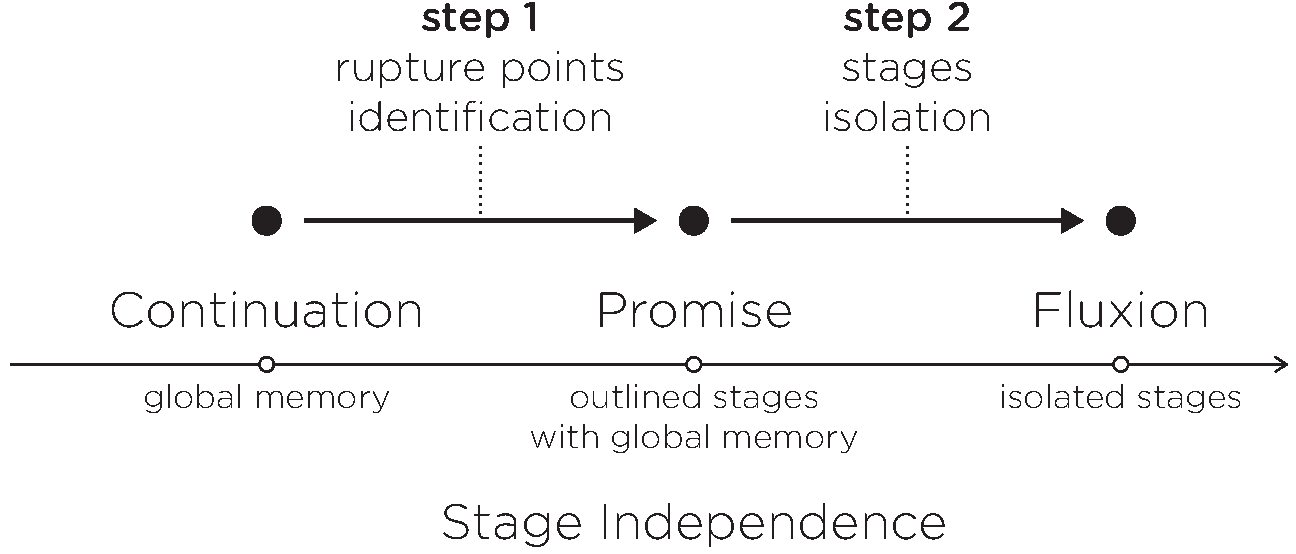
\includegraphics[width=0.7\textwidth]{../resources/roadmap.pdf}%
    \caption{Roadmap}%
    \label{fig:roadmap}%
  }%
\end{figure}

The first compiler focuses on the identification of simple chains of causality between continuations to transform these chains into Promises.
% the transformation from continuations to Promises.
% It focuses on the identification of the chains of causality in continuations.
However, promises are more expressive than the simple chaining of causal sequentiality.
% They force another control over the execution flow.
% According to the outcome of the operation, they call one function to continue the execution with the result, or another to handle errors.
% This conditional execution is indivisible from the Promise specification.
% Promises impose a convention on how to hand back the outcome of the deferred computation, while classic continuations leave this conditional execution to the developer.
Moreover, they impose a different convention than continuations on how to hand back the outcome and errors of the deferred computation.
This difference brings unnecessary complexity to the identification of chains.
To rule out this difference between continuations and Promises, before introducing the first compiler, section \ref{chapter5:due} introduces a simpler specification to Promise, called Due.

The second compiler detects all the chains of causality between continuations and encapsulate them in fluxions.
It isolates the fluxions when possible to allow the parallelism required for efficiency.
This second compilers is introduced in section \ref{chapter5:flx}.

\renewcommand{\glyph}{\iconfont{\XeTeXglyph287}}
\chapter{Implementations} \label{chapter5}
\minitoc
\eject
The transformation allowed by the equivalence from an event-driven program into a distributed network of fluxions is implemented incrementally into two compilers, as presented in figure \ref{fig:roadmap}.
Each compilers is divided into two steps, the identification of the rupture points separating the stages of the pipeline, and the isolation of these stages.
% This chapter presents the technical implementations of these two steps in the transformation from the event-driven execution model to the pipeline architecture
% , the transformation described in the previous chapter was implemented incrementally in two compilers.

\begin{figure}[h!]%
  \textfig{%
    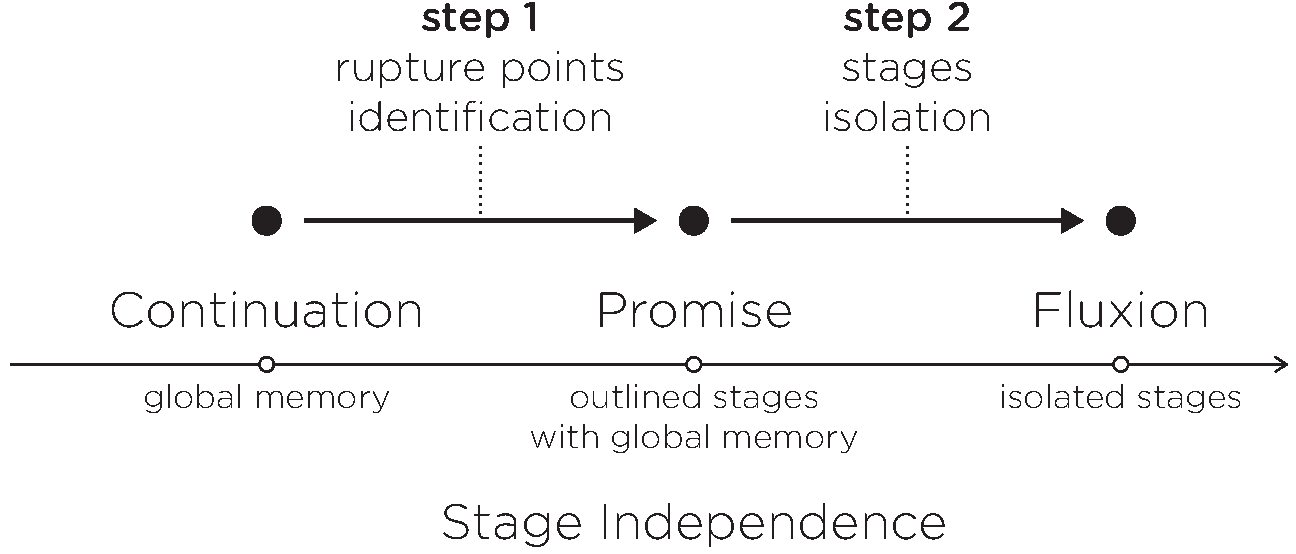
\includegraphics[width=0.7\textwidth]{../resources/roadmap.pdf}%
    \caption{Roadmap}%
    \label{fig:roadmap}%
  }%
\end{figure}

The first compiler focuses on the identification of simple chains of causality between continuations to transform these chains into Promises.
% the transformation from continuations to Promises.
% It focuses on the identification of the chains of causality in continuations.
However, promises are more expressive than the simple chaining of causal sequentiality.
% They force another control over the execution flow.
% According to the outcome of the operation, they call one function to continue the execution with the result, or another to handle errors.
% This conditional execution is indivisible from the Promise specification.
% Promises impose a convention on how to hand back the outcome of the deferred computation, while classic continuations leave this conditional execution to the developer.
Moreover, they impose a different convention than continuations on how to hand back the outcome and errors of the deferred computation.
This difference brings unnecessary complexity to the identification of chains.
To rule out this difference between continuations and Promises, before introducing the first compiler, section \ref{chapter5:due} introduces a simpler specification to Promise, called Due.

The second compiler detects all the chains of causality between continuations and encapsulate them in fluxions.
It isolates the fluxions when possible to allow the parallelism required for efficiency.
This second compilers is introduced in section \ref{chapter5:flx}.

\renewcommand{\glyph}{\iconfont{\XeTeXglyph287}}
\chapter{Implementations} \label{chapter5}
\minitoc
\eject
The transformation allowed by the equivalence from an event-driven program into a distributed network of fluxions is implemented incrementally into two compilers, as presented in figure \ref{fig:roadmap}.
Each compilers is divided into two steps, the identification of the rupture points separating the stages of the pipeline, and the isolation of these stages.
% This chapter presents the technical implementations of these two steps in the transformation from the event-driven execution model to the pipeline architecture
% , the transformation described in the previous chapter was implemented incrementally in two compilers.

\begin{figure}[h!]%
  \textfig{%
    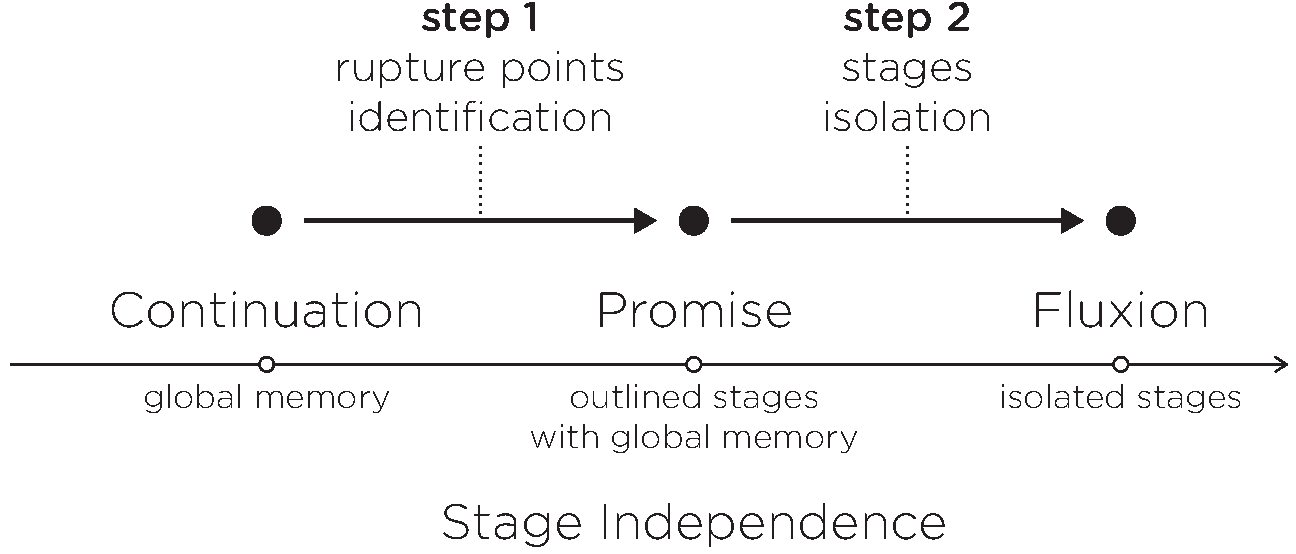
\includegraphics[width=0.7\textwidth]{../resources/roadmap.pdf}%
    \caption{Roadmap}%
    \label{fig:roadmap}%
  }%
\end{figure}

The first compiler focuses on the identification of simple chains of causality between continuations to transform these chains into Promises.
% the transformation from continuations to Promises.
% It focuses on the identification of the chains of causality in continuations.
However, promises are more expressive than the simple chaining of causal sequentiality.
% They force another control over the execution flow.
% According to the outcome of the operation, they call one function to continue the execution with the result, or another to handle errors.
% This conditional execution is indivisible from the Promise specification.
% Promises impose a convention on how to hand back the outcome of the deferred computation, while classic continuations leave this conditional execution to the developer.
Moreover, they impose a different convention than continuations on how to hand back the outcome and errors of the deferred computation.
This difference brings unnecessary complexity to the identification of chains.
To rule out this difference between continuations and Promises, before introducing the first compiler, section \ref{chapter5:due} introduces a simpler specification to Promise, called Due.

The second compiler detects all the chains of causality between continuations and encapsulate them in fluxions.
It isolates the fluxions when possible to allow the parallelism required for efficiency.
This second compilers is introduced in section \ref{chapter5:flx}.

\input{05-implementation/Due/main}
\input{05-implementation/Flx/main}
% \input{05-implementation/Evaluation}

\renewcommand{\glyph}{\iconfont{\XeTeXglyph287}}
\chapter{Implementations} \label{chapter5}
\minitoc
\eject
The transformation allowed by the equivalence from an event-driven program into a distributed network of fluxions is implemented incrementally into two compilers, as presented in figure \ref{fig:roadmap}.
Each compilers is divided into two steps, the identification of the rupture points separating the stages of the pipeline, and the isolation of these stages.
% This chapter presents the technical implementations of these two steps in the transformation from the event-driven execution model to the pipeline architecture
% , the transformation described in the previous chapter was implemented incrementally in two compilers.

\begin{figure}[h!]%
  \textfig{%
    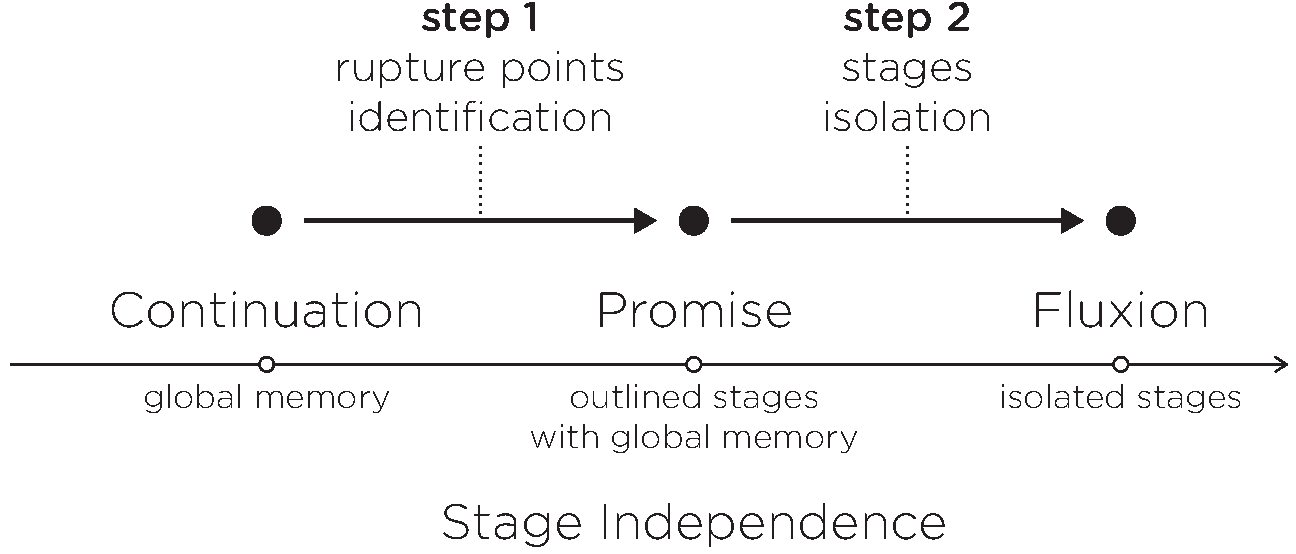
\includegraphics[width=0.7\textwidth]{../resources/roadmap.pdf}%
    \caption{Roadmap}%
    \label{fig:roadmap}%
  }%
\end{figure}

The first compiler focuses on the identification of simple chains of causality between continuations to transform these chains into Promises.
% the transformation from continuations to Promises.
% It focuses on the identification of the chains of causality in continuations.
However, promises are more expressive than the simple chaining of causal sequentiality.
% They force another control over the execution flow.
% According to the outcome of the operation, they call one function to continue the execution with the result, or another to handle errors.
% This conditional execution is indivisible from the Promise specification.
% Promises impose a convention on how to hand back the outcome of the deferred computation, while classic continuations leave this conditional execution to the developer.
Moreover, they impose a different convention than continuations on how to hand back the outcome and errors of the deferred computation.
This difference brings unnecessary complexity to the identification of chains.
To rule out this difference between continuations and Promises, before introducing the first compiler, section \ref{chapter5:due} introduces a simpler specification to Promise, called Due.

The second compiler detects all the chains of causality between continuations and encapsulate them in fluxions.
It isolates the fluxions when possible to allow the parallelism required for efficiency.
This second compilers is introduced in section \ref{chapter5:flx}.

\input{05-implementation/Due/main}
\input{05-implementation/Flx/main}
% \input{05-implementation/Evaluation}

% \subsection{Real test case} \label{chapter5:flx:evaluation}

The compiler is tested on a real application, gifsockets-server\ftnt{https://github.com/twolfson/gifsockets-server}.
This test proves the possibility for an application to be compiled into a network of independent parts.
It shows the current limitations of this isolation and the modifications needed on the application to circumvent them.

\begin{code}[js, caption={Simplified version of gifsockets-server},label={lst:gifsocket}]
var express = require('express'),
    app = express(),
    routes = require('gifsockets-middleware'), //@\label{lst:gifsocket:gif-mw}@
    getRawBody = require('raw-body');

function bodyParser(limit) { //@\label{lst:gifsocket:bodyParser}@
  return function saveBody(req, res, next) { //@\label{lst:gifsocket:saveBody}@
    getRawBody(req, { //@\label{lst:gifsocket:getRawBody}@
      expected: req.headers['content-length'],
      limit: limit
    }, function (err, buffer) { //@\label{lst:gifsocket:callback}@
      req.body = buffer;
      next(); //@\label{lst:gifsocket:next}@
    });
  };
}

app.post('/image/text', bodyParser(1 * 1024 * 1024), routes.writeTextToImages); //@\label{lst:gifsocket:app.post}@
app.listen(8000);
\end{code}

This application, simplified in listing \ref{lst:gifsocket}, is a real-time chat using gif-based communication channels.
It was selected from the evaluation set of the Due compiler because it is simple enough to illustrate this evaluation.
% \cite{Brodu2015}
%  from the \texttt{npm} registry because it depends on \texttt{express}, it is tested, working, and simple enough to illustrate this evaluation.
The server transforms the received text into a gif frame, and pushes it back to a never-ending gif to be displayed on the client.

On line \ref{lst:gifsocket:app.post}, the application registers two functions to process the requests received on the url \texttt{/image/text}.
The closure \texttt{saveBody}, line \ref{lst:gifsocket:saveBody}, returned by \texttt{bodyParser}, line \ref{lst:gifsocket:bodyParser}, and the method \texttt{routes.write\-Text\-To\-Images} from the external module \texttt{gifsockets-\-middleware}, line \ref{lst:gifsocket:gif-mw}.
The closure \texttt{saveBody} calls the asynchronous function \texttt{getRawBody} to get the request body.
Its callback handles the errors, and calls \texttt{next} to continue processing the request with the next function, \texttt{routes.write\-Text\-To\-Images}.

\subsubsection{Compilation} \label{chapter5:flx:evaluation:compilation}

% We compile this application with the compiler
The compilation result is in listing \ref{lst:flx-gifsocket}.
The function call \texttt{app.post}, line \ref{lst:gifsocket:app.post}, is a rupture point.
However, its callbacks, \texttt{bodyParser} and \texttt{routes.write\-Text\-To\-Images} are not declared \textit{in situ}.
They are evaluated as functions only at runtime.
As precised previously, the compiler discards these callbacks to avoid altering the semantic. % by moving or modifying their definition.
% For this reason, the compiler ignores this rupture point, to avoid interfering with the evaluation.

\begin{code}[flx, caption={Compilation result of gifsockets-server},label={lst:flx-gifsocket}]
flx main & express {req}
>> anonymous_1000 [req, next]
  var express = require('express'),
      app = express(),
      routes = require('gifsockets-middleware'), //@\label{lst:flx-gifsocket:gif-mw}@
      getRawBody = require('raw-body');

  function bodyParser(limit) { //@\label{lst:flx-gifsocket:bodyParser}@
    return function saveBody(req, res, next) { //@\label{lst:flx-gifsocket:saveBody}@
      getRawBody(req, { //@\label{lst:flx-gifsocket:getRawBody}@
        expected: req.headers['content-length'], //@\label{lst:flx-gifsocket:req.headers}@
        limit: limit
      }, >> anonymous_1000 [req, next]);
    };
  }

  app.post('/image/text', bodyParser(1 * 1024 * 1024), routes.writeTextToImages); //@\label{lst:flx-gifsocket:app.post}@
  app.listen(8000);

flx anonymous_1000
-> null
  function (err, buffer) { //@\label{lst:flx-gifsocket:callback}@
    req.body = buffer; //@\label{lst:flx-gifsocket:buffer}@
    next(); //@\label{lst:flx-gifsocket:next}@
  }
\end{code}

The compiler detects a rupture point : the function \texttt{get\-Raw\-Body} and its anonymous callback, line \ref{lst:gifsocket:callback}.
It encapsulates this callback in a fluxion named \texttt{anony\-mous\_\-1000}.
The callback is replaced with a stream placeholder to send the message stream to this downstream fluxion.
The variables \texttt{req} and \texttt{next} are appended to this message stream, to propagate their value from the \texttt{main} fluxion to the \texttt{anony\-mous\_\-1000} fluxion.

When \texttt{anony\-mous\_\-1000} is not isolated from the \texttt{main} fluxion, as if they belong to the same group, the compilation result works as expected.
The variables used in the fluxion, \texttt{req} and \texttt{next}, are still shared between the two fluxions.
In this situation fluxions are quite similar to Dues regarding memory shareing.
Our goal is to isolate the two fluxions, to be able to safely parallelize their executions.

\subsubsection{Isolation} \label{chapter5:flx:evaluation:isolation}

In listing \ref{lst:flx-gifsocket}, the fluxion \texttt{anony\-mous\_\-1000} modifies the object \texttt{req}, line \ref{lst:flx-gifsocket:buffer}, to store the text of the received request, and it calls \texttt{next} to continue the execution, line \ref{lst:flx-gifsocket:next}.
\texttt{req} is an alias to a memory location used in multiple palces in code.
Therefore, these operations produce side-effects that should propagate in the whole application, but the isolation prevents this propagation.
Isolating the fluxion \texttt{anony\-mous\_\-1000} produces runtime exceptions.
The next paragraph details how this situation is handled to allow the application to be parallelized.

\paragraph{Variable \texttt{req}}

The variable \texttt{req} is read in fluxion \texttt{main}, lines \ref{lst:flx-gifsocket:getRawBody} and \ref{lst:flx-gifsocket:req.headers}.
Then its property \texttt{body} is associated to \texttt{buffer} in fluxion \texttt{anony\-mous\_\-1000}, line \ref{lst:flx-gifsocket:buffer}.
The compiler is unable to identify the aliases of this variable. % further usages.
However, the side effect resulting from this association impacts a variable in the scope of the next callback, \texttt{routes.write\-Text\-To\-Images}.
In this test case, the application is modified manually to explicitly propagate this side-effect to the next callback through the function \texttt{next}.
The modifications of this function are explained further in the next paragraph.

\paragraph{Closure \texttt{next}}

The function \texttt{next} is a closure provided by the \texttt{express} \texttt{Router} to continue the execution with the next function to handle the client request.
Because it indirectly relies on the variable \texttt{req}, it is impossible to isolate its execution with the \texttt{anony\-mous\_\-1000} fluxion.
Instead, we modify \texttt{express}, so as to be compatible with the fluxional execution model.
We explain the modifications below.

\begin{code}[flx, caption={Simplified modification on the compiled result},label={lst:mflx-gifsocket}]
flx anonymous_1000
-> express_dispatcher
  function (err, buffer) { //@\label{lst:mflx-gifsocket:callback}@
    req.body = buffer; //@\label{lst:mflx-gifsocket:buffer}@
    next_placeholder(req, -> express_dispatcher); //@\label{lst:mflx-gifsocket:next-placeholder}@
  }

flx express_dispatcher & express {req} //@\label{lst:mflx-gifsocket:express-dispatcher}@
-> null
  function (modified_req) {
    merge(req, modified_req);
    next(); //@\label{lst:mflx-gifsocket:next}@
  }
\end{code}

In listing \ref{lst:gifsocket}, the function \texttt{next} is a continuation allowing the anonymous callback, line \ref{lst:gifsocket:callback}, to call the next function to handle the request.
To isolate the anonymous callback into \texttt{anonymous\_\-1000}, \texttt{next} is replaced by a rupture point.
This replacement is illustrated in listing \ref{lst:mflx-gifsocket}.
The \texttt{express} \texttt{Router} registers a fluxion named \texttt{express\_\-dispatcher}, line \ref{lst:mflx-gifsocket:express-dispatcher}, to continue the execution after the fluxion \texttt{anony\-mous\_\-1000}.
This fluxion is in the same group \texttt{express} as the \texttt{main} fluxion, hence it has access to the original variable \texttt{req}, and to the original function \texttt{next}.
The call to the original \texttt{next} function is replaced by a placeholder to push the stream to the fluxion \texttt{express\_\-dispatcher}, line \ref{lst:mflx-gifsocket:next-placeholder}.
The fluxion \texttt{express\_\-dispatcher} receives the stream from the upstream fluxion \texttt{anony\-mous\_\-1000}, merges back the modification in the variable \texttt{req} to propagate the side effects, and finally calls the original function \texttt{next} to continue the execution, line \ref{lst:mflx-gifsocket:next}.

After the modifications detailed above, the server works as expected.
The isolated fluxion correctly receives, and returns its serialized messages.
The client successfully receives a gif frame containing the text.



\subsection{Limitations}

The static analysis used for this compiler presents some limitations.
It is unable to analyze code with dynamic behaviors.
Higher-order programming leads to more productivity partly beacuse it rely on such dynamic behavior to extend expressivity.
Precisely, it allows more levels of indirections.

\subsubsection{Levels of Indirections}

The indirection is an abstraction between the value, and its manipulation.
In listing \ref{lst:indirection}, the variables \texttt{a} and \texttt{b} point both to the same memory object.
The function \texttt{fn} introduces a level of indirection between the real object \texttt{a} and its manipulation handle, \texttt{b};
% Actually, the variable \texttt{a} already introduces a level of indirection between the real object and the handle \texttt{a}.

\begin{code}[js,
  caption={One level of Indirection},
  label={lst:indirection}]
var a = {
      // an object;
    };

fn(b) {
  // modify b;
}

fn(a);
\end{code}

\subsubsection{Uncertainties}

The indirection is trivial to resolve in listing \ref{lst:indirection}.
It only needs to have access to the definition of \texttt{a} and of \texttt{fn}.
%A very simple static analysis could resolve it.
However, in listing \ref{lst:indirections}, the array \texttt{handlers} introduces a new level of indirection.
The static analysis now needs to have access to the definition of \texttt{i} and of the \texttt{handlers}.
If this definition is provided by an external input, it is not available statically, hence, it adds an uncertainty during the analysis. 

\begin{code}[js,
  caption={Two levels of indirection},
  label={lst:indirections}]
var a = {
      // an object;
    },
    handlers = [
      // definition of fn handlers;
    ],
    i = ?;

handlers[i](a);
handlers[i+1](a);
\end{code}

These examples are extremely simplified.
A real application contains enough indirections for the static analysis to be overwhelmed by uncertainties, and to be unable to resolve the variables.
If a variable is left unresolved, it is impossible to assure its scope and its aliases.
Therefore, the compiler is unable to isolate it into a fluxion, or to distribute its modification by messages.

Moreover, it leads the compiler to ignore the rupture points not defined \textit{in situ}, because their modifications could impact the semantic.
The reason for this precaution, is that the compiler is unable to assure where the function is used, and the scope of its variables.
Therefore, it is unable to assure that the modification will conserve the semantic.

\subsubsection{Dynamic Resolution}

In a web application, this variable \texttt{i} might be part of the user request, which is available only at runtime.
It eventually introduces an uncertainty.

This dynamic resolution of variables is precisely what increase expressiveness.
Trying to resolve them statically is equivalent to restrict expressiveness.
No static analysis can overstep these limitations.
Only a dynamic analysis could analysis the resolved indirections during run time to overstep these limitations correctly.




\renewcommand{\glyph}{\iconfont{\XeTeXglyph287}}
\chapter{Implementations} \label{chapter5}
\minitoc
\eject
The transformation allowed by the equivalence from an event-driven program into a distributed network of fluxions is implemented incrementally into two compilers, as presented in figure \ref{fig:roadmap}.
Each compilers is divided into two steps, the identification of the rupture points separating the stages of the pipeline, and the isolation of these stages.
% This chapter presents the technical implementations of these two steps in the transformation from the event-driven execution model to the pipeline architecture
% , the transformation described in the previous chapter was implemented incrementally in two compilers.

\begin{figure}[h!]%
  \textfig{%
    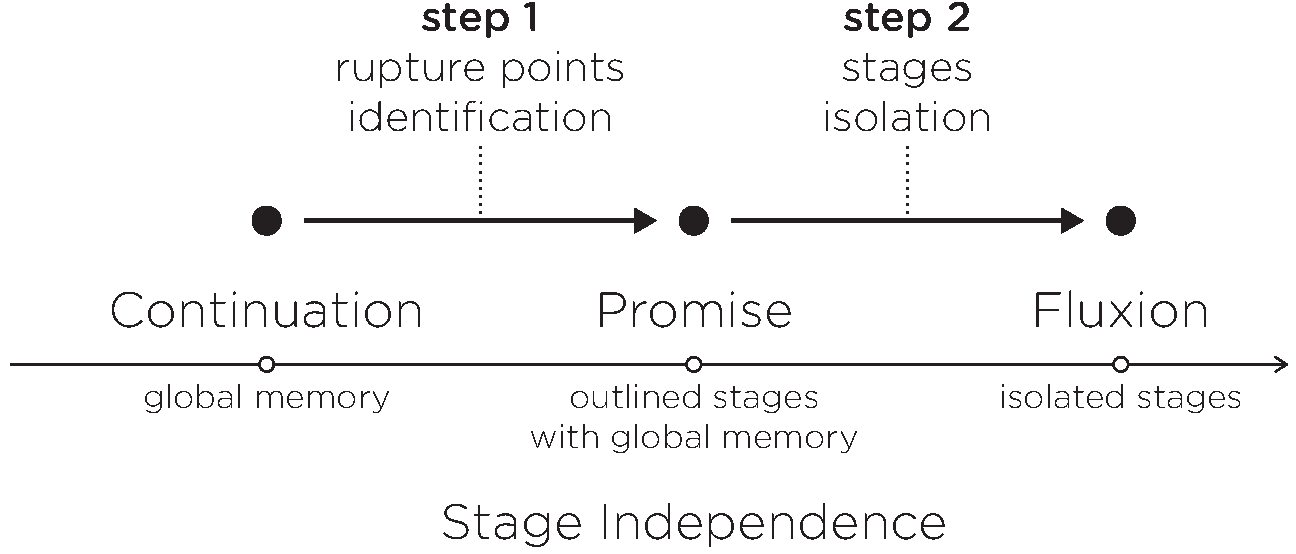
\includegraphics[width=0.7\textwidth]{../resources/roadmap.pdf}%
    \caption{Roadmap}%
    \label{fig:roadmap}%
  }%
\end{figure}

The first compiler focuses on the identification of simple chains of causality between continuations to transform these chains into Promises.
% the transformation from continuations to Promises.
% It focuses on the identification of the chains of causality in continuations.
However, promises are more expressive than the simple chaining of causal sequentiality.
% They force another control over the execution flow.
% According to the outcome of the operation, they call one function to continue the execution with the result, or another to handle errors.
% This conditional execution is indivisible from the Promise specification.
% Promises impose a convention on how to hand back the outcome of the deferred computation, while classic continuations leave this conditional execution to the developer.
Moreover, they impose a different convention than continuations on how to hand back the outcome and errors of the deferred computation.
This difference brings unnecessary complexity to the identification of chains.
To rule out this difference between continuations and Promises, before introducing the first compiler, section \ref{chapter5:due} introduces a simpler specification to Promise, called Due.

The second compiler detects all the chains of causality between continuations and encapsulate them in fluxions.
It isolates the fluxions when possible to allow the parallelism required for efficiency.
This second compilers is introduced in section \ref{chapter5:flx}.

\renewcommand{\glyph}{\iconfont{\XeTeXglyph287}}
\chapter{Implementations} \label{chapter5}
\minitoc
\eject
The transformation allowed by the equivalence from an event-driven program into a distributed network of fluxions is implemented incrementally into two compilers, as presented in figure \ref{fig:roadmap}.
Each compilers is divided into two steps, the identification of the rupture points separating the stages of the pipeline, and the isolation of these stages.
% This chapter presents the technical implementations of these two steps in the transformation from the event-driven execution model to the pipeline architecture
% , the transformation described in the previous chapter was implemented incrementally in two compilers.

\begin{figure}[h!]%
  \textfig{%
    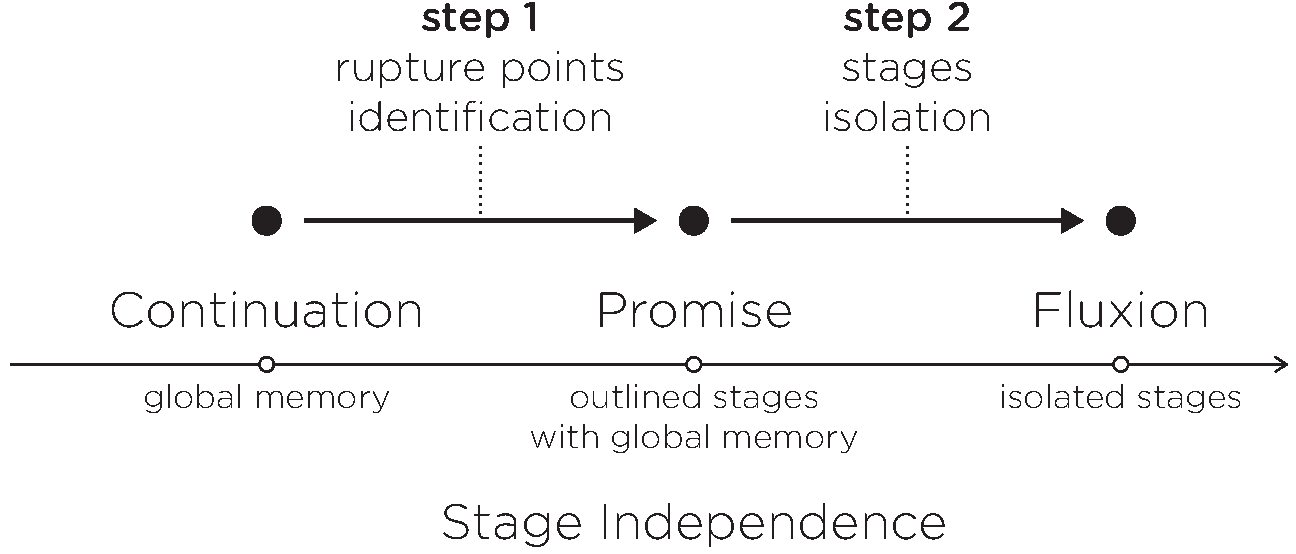
\includegraphics[width=0.7\textwidth]{../resources/roadmap.pdf}%
    \caption{Roadmap}%
    \label{fig:roadmap}%
  }%
\end{figure}

The first compiler focuses on the identification of simple chains of causality between continuations to transform these chains into Promises.
% the transformation from continuations to Promises.
% It focuses on the identification of the chains of causality in continuations.
However, promises are more expressive than the simple chaining of causal sequentiality.
% They force another control over the execution flow.
% According to the outcome of the operation, they call one function to continue the execution with the result, or another to handle errors.
% This conditional execution is indivisible from the Promise specification.
% Promises impose a convention on how to hand back the outcome of the deferred computation, while classic continuations leave this conditional execution to the developer.
Moreover, they impose a different convention than continuations on how to hand back the outcome and errors of the deferred computation.
This difference brings unnecessary complexity to the identification of chains.
To rule out this difference between continuations and Promises, before introducing the first compiler, section \ref{chapter5:due} introduces a simpler specification to Promise, called Due.

The second compiler detects all the chains of causality between continuations and encapsulate them in fluxions.
It isolates the fluxions when possible to allow the parallelism required for efficiency.
This second compilers is introduced in section \ref{chapter5:flx}.

\input{05-implementation/Due/main}
\input{05-implementation/Flx/main}
% \input{05-implementation/Evaluation}

\renewcommand{\glyph}{\iconfont{\XeTeXglyph287}}
\chapter{Implementations} \label{chapter5}
\minitoc
\eject
The transformation allowed by the equivalence from an event-driven program into a distributed network of fluxions is implemented incrementally into two compilers, as presented in figure \ref{fig:roadmap}.
Each compilers is divided into two steps, the identification of the rupture points separating the stages of the pipeline, and the isolation of these stages.
% This chapter presents the technical implementations of these two steps in the transformation from the event-driven execution model to the pipeline architecture
% , the transformation described in the previous chapter was implemented incrementally in two compilers.

\begin{figure}[h!]%
  \textfig{%
    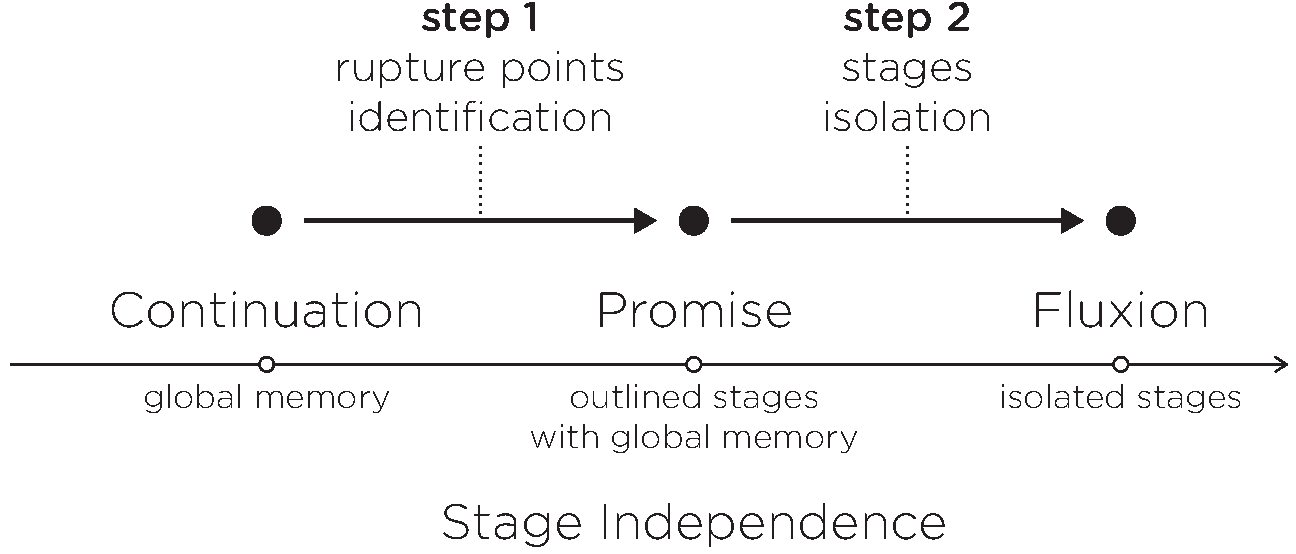
\includegraphics[width=0.7\textwidth]{../resources/roadmap.pdf}%
    \caption{Roadmap}%
    \label{fig:roadmap}%
  }%
\end{figure}

The first compiler focuses on the identification of simple chains of causality between continuations to transform these chains into Promises.
% the transformation from continuations to Promises.
% It focuses on the identification of the chains of causality in continuations.
However, promises are more expressive than the simple chaining of causal sequentiality.
% They force another control over the execution flow.
% According to the outcome of the operation, they call one function to continue the execution with the result, or another to handle errors.
% This conditional execution is indivisible from the Promise specification.
% Promises impose a convention on how to hand back the outcome of the deferred computation, while classic continuations leave this conditional execution to the developer.
Moreover, they impose a different convention than continuations on how to hand back the outcome and errors of the deferred computation.
This difference brings unnecessary complexity to the identification of chains.
To rule out this difference between continuations and Promises, before introducing the first compiler, section \ref{chapter5:due} introduces a simpler specification to Promise, called Due.

The second compiler detects all the chains of causality between continuations and encapsulate them in fluxions.
It isolates the fluxions when possible to allow the parallelism required for efficiency.
This second compilers is introduced in section \ref{chapter5:flx}.

\input{05-implementation/Due/main}
\input{05-implementation/Flx/main}
% \input{05-implementation/Evaluation}

% \subsection{Real test case} \label{chapter5:flx:evaluation}

The compiler is tested on a real application, gifsockets-server\ftnt{https://github.com/twolfson/gifsockets-server}.
This test proves the possibility for an application to be compiled into a network of independent parts.
It shows the current limitations of this isolation and the modifications needed on the application to circumvent them.

\begin{code}[js, caption={Simplified version of gifsockets-server},label={lst:gifsocket}]
var express = require('express'),
    app = express(),
    routes = require('gifsockets-middleware'), //@\label{lst:gifsocket:gif-mw}@
    getRawBody = require('raw-body');

function bodyParser(limit) { //@\label{lst:gifsocket:bodyParser}@
  return function saveBody(req, res, next) { //@\label{lst:gifsocket:saveBody}@
    getRawBody(req, { //@\label{lst:gifsocket:getRawBody}@
      expected: req.headers['content-length'],
      limit: limit
    }, function (err, buffer) { //@\label{lst:gifsocket:callback}@
      req.body = buffer;
      next(); //@\label{lst:gifsocket:next}@
    });
  };
}

app.post('/image/text', bodyParser(1 * 1024 * 1024), routes.writeTextToImages); //@\label{lst:gifsocket:app.post}@
app.listen(8000);
\end{code}

This application, simplified in listing \ref{lst:gifsocket}, is a real-time chat using gif-based communication channels.
It was selected from the evaluation set of the Due compiler because it is simple enough to illustrate this evaluation.
% \cite{Brodu2015}
%  from the \texttt{npm} registry because it depends on \texttt{express}, it is tested, working, and simple enough to illustrate this evaluation.
The server transforms the received text into a gif frame, and pushes it back to a never-ending gif to be displayed on the client.

On line \ref{lst:gifsocket:app.post}, the application registers two functions to process the requests received on the url \texttt{/image/text}.
The closure \texttt{saveBody}, line \ref{lst:gifsocket:saveBody}, returned by \texttt{bodyParser}, line \ref{lst:gifsocket:bodyParser}, and the method \texttt{routes.write\-Text\-To\-Images} from the external module \texttt{gifsockets-\-middleware}, line \ref{lst:gifsocket:gif-mw}.
The closure \texttt{saveBody} calls the asynchronous function \texttt{getRawBody} to get the request body.
Its callback handles the errors, and calls \texttt{next} to continue processing the request with the next function, \texttt{routes.write\-Text\-To\-Images}.

\subsubsection{Compilation} \label{chapter5:flx:evaluation:compilation}

% We compile this application with the compiler
The compilation result is in listing \ref{lst:flx-gifsocket}.
The function call \texttt{app.post}, line \ref{lst:gifsocket:app.post}, is a rupture point.
However, its callbacks, \texttt{bodyParser} and \texttt{routes.write\-Text\-To\-Images} are not declared \textit{in situ}.
They are evaluated as functions only at runtime.
As precised previously, the compiler discards these callbacks to avoid altering the semantic. % by moving or modifying their definition.
% For this reason, the compiler ignores this rupture point, to avoid interfering with the evaluation.

\begin{code}[flx, caption={Compilation result of gifsockets-server},label={lst:flx-gifsocket}]
flx main & express {req}
>> anonymous_1000 [req, next]
  var express = require('express'),
      app = express(),
      routes = require('gifsockets-middleware'), //@\label{lst:flx-gifsocket:gif-mw}@
      getRawBody = require('raw-body');

  function bodyParser(limit) { //@\label{lst:flx-gifsocket:bodyParser}@
    return function saveBody(req, res, next) { //@\label{lst:flx-gifsocket:saveBody}@
      getRawBody(req, { //@\label{lst:flx-gifsocket:getRawBody}@
        expected: req.headers['content-length'], //@\label{lst:flx-gifsocket:req.headers}@
        limit: limit
      }, >> anonymous_1000 [req, next]);
    };
  }

  app.post('/image/text', bodyParser(1 * 1024 * 1024), routes.writeTextToImages); //@\label{lst:flx-gifsocket:app.post}@
  app.listen(8000);

flx anonymous_1000
-> null
  function (err, buffer) { //@\label{lst:flx-gifsocket:callback}@
    req.body = buffer; //@\label{lst:flx-gifsocket:buffer}@
    next(); //@\label{lst:flx-gifsocket:next}@
  }
\end{code}

The compiler detects a rupture point : the function \texttt{get\-Raw\-Body} and its anonymous callback, line \ref{lst:gifsocket:callback}.
It encapsulates this callback in a fluxion named \texttt{anony\-mous\_\-1000}.
The callback is replaced with a stream placeholder to send the message stream to this downstream fluxion.
The variables \texttt{req} and \texttt{next} are appended to this message stream, to propagate their value from the \texttt{main} fluxion to the \texttt{anony\-mous\_\-1000} fluxion.

When \texttt{anony\-mous\_\-1000} is not isolated from the \texttt{main} fluxion, as if they belong to the same group, the compilation result works as expected.
The variables used in the fluxion, \texttt{req} and \texttt{next}, are still shared between the two fluxions.
In this situation fluxions are quite similar to Dues regarding memory shareing.
Our goal is to isolate the two fluxions, to be able to safely parallelize their executions.

\subsubsection{Isolation} \label{chapter5:flx:evaluation:isolation}

In listing \ref{lst:flx-gifsocket}, the fluxion \texttt{anony\-mous\_\-1000} modifies the object \texttt{req}, line \ref{lst:flx-gifsocket:buffer}, to store the text of the received request, and it calls \texttt{next} to continue the execution, line \ref{lst:flx-gifsocket:next}.
\texttt{req} is an alias to a memory location used in multiple palces in code.
Therefore, these operations produce side-effects that should propagate in the whole application, but the isolation prevents this propagation.
Isolating the fluxion \texttt{anony\-mous\_\-1000} produces runtime exceptions.
The next paragraph details how this situation is handled to allow the application to be parallelized.

\paragraph{Variable \texttt{req}}

The variable \texttt{req} is read in fluxion \texttt{main}, lines \ref{lst:flx-gifsocket:getRawBody} and \ref{lst:flx-gifsocket:req.headers}.
Then its property \texttt{body} is associated to \texttt{buffer} in fluxion \texttt{anony\-mous\_\-1000}, line \ref{lst:flx-gifsocket:buffer}.
The compiler is unable to identify the aliases of this variable. % further usages.
However, the side effect resulting from this association impacts a variable in the scope of the next callback, \texttt{routes.write\-Text\-To\-Images}.
In this test case, the application is modified manually to explicitly propagate this side-effect to the next callback through the function \texttt{next}.
The modifications of this function are explained further in the next paragraph.

\paragraph{Closure \texttt{next}}

The function \texttt{next} is a closure provided by the \texttt{express} \texttt{Router} to continue the execution with the next function to handle the client request.
Because it indirectly relies on the variable \texttt{req}, it is impossible to isolate its execution with the \texttt{anony\-mous\_\-1000} fluxion.
Instead, we modify \texttt{express}, so as to be compatible with the fluxional execution model.
We explain the modifications below.

\begin{code}[flx, caption={Simplified modification on the compiled result},label={lst:mflx-gifsocket}]
flx anonymous_1000
-> express_dispatcher
  function (err, buffer) { //@\label{lst:mflx-gifsocket:callback}@
    req.body = buffer; //@\label{lst:mflx-gifsocket:buffer}@
    next_placeholder(req, -> express_dispatcher); //@\label{lst:mflx-gifsocket:next-placeholder}@
  }

flx express_dispatcher & express {req} //@\label{lst:mflx-gifsocket:express-dispatcher}@
-> null
  function (modified_req) {
    merge(req, modified_req);
    next(); //@\label{lst:mflx-gifsocket:next}@
  }
\end{code}

In listing \ref{lst:gifsocket}, the function \texttt{next} is a continuation allowing the anonymous callback, line \ref{lst:gifsocket:callback}, to call the next function to handle the request.
To isolate the anonymous callback into \texttt{anonymous\_\-1000}, \texttt{next} is replaced by a rupture point.
This replacement is illustrated in listing \ref{lst:mflx-gifsocket}.
The \texttt{express} \texttt{Router} registers a fluxion named \texttt{express\_\-dispatcher}, line \ref{lst:mflx-gifsocket:express-dispatcher}, to continue the execution after the fluxion \texttt{anony\-mous\_\-1000}.
This fluxion is in the same group \texttt{express} as the \texttt{main} fluxion, hence it has access to the original variable \texttt{req}, and to the original function \texttt{next}.
The call to the original \texttt{next} function is replaced by a placeholder to push the stream to the fluxion \texttt{express\_\-dispatcher}, line \ref{lst:mflx-gifsocket:next-placeholder}.
The fluxion \texttt{express\_\-dispatcher} receives the stream from the upstream fluxion \texttt{anony\-mous\_\-1000}, merges back the modification in the variable \texttt{req} to propagate the side effects, and finally calls the original function \texttt{next} to continue the execution, line \ref{lst:mflx-gifsocket:next}.

After the modifications detailed above, the server works as expected.
The isolated fluxion correctly receives, and returns its serialized messages.
The client successfully receives a gif frame containing the text.



\subsection{Limitations}

The static analysis used for this compiler presents some limitations.
It is unable to analyze code with dynamic behaviors.
Higher-order programming leads to more productivity partly beacuse it rely on such dynamic behavior to extend expressivity.
Precisely, it allows more levels of indirections.

\subsubsection{Levels of Indirections}

The indirection is an abstraction between the value, and its manipulation.
In listing \ref{lst:indirection}, the variables \texttt{a} and \texttt{b} point both to the same memory object.
The function \texttt{fn} introduces a level of indirection between the real object \texttt{a} and its manipulation handle, \texttt{b};
% Actually, the variable \texttt{a} already introduces a level of indirection between the real object and the handle \texttt{a}.

\begin{code}[js,
  caption={One level of Indirection},
  label={lst:indirection}]
var a = {
      // an object;
    };

fn(b) {
  // modify b;
}

fn(a);
\end{code}

\subsubsection{Uncertainties}

The indirection is trivial to resolve in listing \ref{lst:indirection}.
It only needs to have access to the definition of \texttt{a} and of \texttt{fn}.
%A very simple static analysis could resolve it.
However, in listing \ref{lst:indirections}, the array \texttt{handlers} introduces a new level of indirection.
The static analysis now needs to have access to the definition of \texttt{i} and of the \texttt{handlers}.
If this definition is provided by an external input, it is not available statically, hence, it adds an uncertainty during the analysis. 

\begin{code}[js,
  caption={Two levels of indirection},
  label={lst:indirections}]
var a = {
      // an object;
    },
    handlers = [
      // definition of fn handlers;
    ],
    i = ?;

handlers[i](a);
handlers[i+1](a);
\end{code}

These examples are extremely simplified.
A real application contains enough indirections for the static analysis to be overwhelmed by uncertainties, and to be unable to resolve the variables.
If a variable is left unresolved, it is impossible to assure its scope and its aliases.
Therefore, the compiler is unable to isolate it into a fluxion, or to distribute its modification by messages.

Moreover, it leads the compiler to ignore the rupture points not defined \textit{in situ}, because their modifications could impact the semantic.
The reason for this precaution, is that the compiler is unable to assure where the function is used, and the scope of its variables.
Therefore, it is unable to assure that the modification will conserve the semantic.

\subsubsection{Dynamic Resolution}

In a web application, this variable \texttt{i} might be part of the user request, which is available only at runtime.
It eventually introduces an uncertainty.

This dynamic resolution of variables is precisely what increase expressiveness.
Trying to resolve them statically is equivalent to restrict expressiveness.
No static analysis can overstep these limitations.
Only a dynamic analysis could analysis the resolved indirections during run time to overstep these limitations correctly.




% \subsection{Real test case} \label{chapter5:flx:evaluation}

The compiler is tested on a real application, gifsockets-server\ftnt{https://github.com/twolfson/gifsockets-server}.
This test proves the possibility for an application to be compiled into a network of independent parts.
It shows the current limitations of this isolation and the modifications needed on the application to circumvent them.

\begin{code}[js, caption={Simplified version of gifsockets-server},label={lst:gifsocket}]
var express = require('express'),
    app = express(),
    routes = require('gifsockets-middleware'), //@\label{lst:gifsocket:gif-mw}@
    getRawBody = require('raw-body');

function bodyParser(limit) { //@\label{lst:gifsocket:bodyParser}@
  return function saveBody(req, res, next) { //@\label{lst:gifsocket:saveBody}@
    getRawBody(req, { //@\label{lst:gifsocket:getRawBody}@
      expected: req.headers['content-length'],
      limit: limit
    }, function (err, buffer) { //@\label{lst:gifsocket:callback}@
      req.body = buffer;
      next(); //@\label{lst:gifsocket:next}@
    });
  };
}

app.post('/image/text', bodyParser(1 * 1024 * 1024), routes.writeTextToImages); //@\label{lst:gifsocket:app.post}@
app.listen(8000);
\end{code}

This application, simplified in listing \ref{lst:gifsocket}, is a real-time chat using gif-based communication channels.
It was selected from the evaluation set of the Due compiler because it is simple enough to illustrate this evaluation.
% \cite{Brodu2015}
%  from the \texttt{npm} registry because it depends on \texttt{express}, it is tested, working, and simple enough to illustrate this evaluation.
The server transforms the received text into a gif frame, and pushes it back to a never-ending gif to be displayed on the client.

On line \ref{lst:gifsocket:app.post}, the application registers two functions to process the requests received on the url \texttt{/image/text}.
The closure \texttt{saveBody}, line \ref{lst:gifsocket:saveBody}, returned by \texttt{bodyParser}, line \ref{lst:gifsocket:bodyParser}, and the method \texttt{routes.write\-Text\-To\-Images} from the external module \texttt{gifsockets-\-middleware}, line \ref{lst:gifsocket:gif-mw}.
The closure \texttt{saveBody} calls the asynchronous function \texttt{getRawBody} to get the request body.
Its callback handles the errors, and calls \texttt{next} to continue processing the request with the next function, \texttt{routes.write\-Text\-To\-Images}.

\subsubsection{Compilation} \label{chapter5:flx:evaluation:compilation}

% We compile this application with the compiler
The compilation result is in listing \ref{lst:flx-gifsocket}.
The function call \texttt{app.post}, line \ref{lst:gifsocket:app.post}, is a rupture point.
However, its callbacks, \texttt{bodyParser} and \texttt{routes.write\-Text\-To\-Images} are not declared \textit{in situ}.
They are evaluated as functions only at runtime.
As precised previously, the compiler discards these callbacks to avoid altering the semantic. % by moving or modifying their definition.
% For this reason, the compiler ignores this rupture point, to avoid interfering with the evaluation.

\begin{code}[flx, caption={Compilation result of gifsockets-server},label={lst:flx-gifsocket}]
flx main & express {req}
>> anonymous_1000 [req, next]
  var express = require('express'),
      app = express(),
      routes = require('gifsockets-middleware'), //@\label{lst:flx-gifsocket:gif-mw}@
      getRawBody = require('raw-body');

  function bodyParser(limit) { //@\label{lst:flx-gifsocket:bodyParser}@
    return function saveBody(req, res, next) { //@\label{lst:flx-gifsocket:saveBody}@
      getRawBody(req, { //@\label{lst:flx-gifsocket:getRawBody}@
        expected: req.headers['content-length'], //@\label{lst:flx-gifsocket:req.headers}@
        limit: limit
      }, >> anonymous_1000 [req, next]);
    };
  }

  app.post('/image/text', bodyParser(1 * 1024 * 1024), routes.writeTextToImages); //@\label{lst:flx-gifsocket:app.post}@
  app.listen(8000);

flx anonymous_1000
-> null
  function (err, buffer) { //@\label{lst:flx-gifsocket:callback}@
    req.body = buffer; //@\label{lst:flx-gifsocket:buffer}@
    next(); //@\label{lst:flx-gifsocket:next}@
  }
\end{code}

The compiler detects a rupture point : the function \texttt{get\-Raw\-Body} and its anonymous callback, line \ref{lst:gifsocket:callback}.
It encapsulates this callback in a fluxion named \texttt{anony\-mous\_\-1000}.
The callback is replaced with a stream placeholder to send the message stream to this downstream fluxion.
The variables \texttt{req} and \texttt{next} are appended to this message stream, to propagate their value from the \texttt{main} fluxion to the \texttt{anony\-mous\_\-1000} fluxion.

When \texttt{anony\-mous\_\-1000} is not isolated from the \texttt{main} fluxion, as if they belong to the same group, the compilation result works as expected.
The variables used in the fluxion, \texttt{req} and \texttt{next}, are still shared between the two fluxions.
In this situation fluxions are quite similar to Dues regarding memory shareing.
Our goal is to isolate the two fluxions, to be able to safely parallelize their executions.

\subsubsection{Isolation} \label{chapter5:flx:evaluation:isolation}

In listing \ref{lst:flx-gifsocket}, the fluxion \texttt{anony\-mous\_\-1000} modifies the object \texttt{req}, line \ref{lst:flx-gifsocket:buffer}, to store the text of the received request, and it calls \texttt{next} to continue the execution, line \ref{lst:flx-gifsocket:next}.
\texttt{req} is an alias to a memory location used in multiple palces in code.
Therefore, these operations produce side-effects that should propagate in the whole application, but the isolation prevents this propagation.
Isolating the fluxion \texttt{anony\-mous\_\-1000} produces runtime exceptions.
The next paragraph details how this situation is handled to allow the application to be parallelized.

\paragraph{Variable \texttt{req}}

The variable \texttt{req} is read in fluxion \texttt{main}, lines \ref{lst:flx-gifsocket:getRawBody} and \ref{lst:flx-gifsocket:req.headers}.
Then its property \texttt{body} is associated to \texttt{buffer} in fluxion \texttt{anony\-mous\_\-1000}, line \ref{lst:flx-gifsocket:buffer}.
The compiler is unable to identify the aliases of this variable. % further usages.
However, the side effect resulting from this association impacts a variable in the scope of the next callback, \texttt{routes.write\-Text\-To\-Images}.
In this test case, the application is modified manually to explicitly propagate this side-effect to the next callback through the function \texttt{next}.
The modifications of this function are explained further in the next paragraph.

\paragraph{Closure \texttt{next}}

The function \texttt{next} is a closure provided by the \texttt{express} \texttt{Router} to continue the execution with the next function to handle the client request.
Because it indirectly relies on the variable \texttt{req}, it is impossible to isolate its execution with the \texttt{anony\-mous\_\-1000} fluxion.
Instead, we modify \texttt{express}, so as to be compatible with the fluxional execution model.
We explain the modifications below.

\begin{code}[flx, caption={Simplified modification on the compiled result},label={lst:mflx-gifsocket}]
flx anonymous_1000
-> express_dispatcher
  function (err, buffer) { //@\label{lst:mflx-gifsocket:callback}@
    req.body = buffer; //@\label{lst:mflx-gifsocket:buffer}@
    next_placeholder(req, -> express_dispatcher); //@\label{lst:mflx-gifsocket:next-placeholder}@
  }

flx express_dispatcher & express {req} //@\label{lst:mflx-gifsocket:express-dispatcher}@
-> null
  function (modified_req) {
    merge(req, modified_req);
    next(); //@\label{lst:mflx-gifsocket:next}@
  }
\end{code}

In listing \ref{lst:gifsocket}, the function \texttt{next} is a continuation allowing the anonymous callback, line \ref{lst:gifsocket:callback}, to call the next function to handle the request.
To isolate the anonymous callback into \texttt{anonymous\_\-1000}, \texttt{next} is replaced by a rupture point.
This replacement is illustrated in listing \ref{lst:mflx-gifsocket}.
The \texttt{express} \texttt{Router} registers a fluxion named \texttt{express\_\-dispatcher}, line \ref{lst:mflx-gifsocket:express-dispatcher}, to continue the execution after the fluxion \texttt{anony\-mous\_\-1000}.
This fluxion is in the same group \texttt{express} as the \texttt{main} fluxion, hence it has access to the original variable \texttt{req}, and to the original function \texttt{next}.
The call to the original \texttt{next} function is replaced by a placeholder to push the stream to the fluxion \texttt{express\_\-dispatcher}, line \ref{lst:mflx-gifsocket:next-placeholder}.
The fluxion \texttt{express\_\-dispatcher} receives the stream from the upstream fluxion \texttt{anony\-mous\_\-1000}, merges back the modification in the variable \texttt{req} to propagate the side effects, and finally calls the original function \texttt{next} to continue the execution, line \ref{lst:mflx-gifsocket:next}.

After the modifications detailed above, the server works as expected.
The isolated fluxion correctly receives, and returns its serialized messages.
The client successfully receives a gif frame containing the text.



\subsection{Limitations}

The static analysis used for this compiler presents some limitations.
It is unable to analyze code with dynamic behaviors.
Higher-order programming leads to more productivity partly beacuse it rely on such dynamic behavior to extend expressivity.
Precisely, it allows more levels of indirections.

\subsubsection{Levels of Indirections}

The indirection is an abstraction between the value, and its manipulation.
In listing \ref{lst:indirection}, the variables \texttt{a} and \texttt{b} point both to the same memory object.
The function \texttt{fn} introduces a level of indirection between the real object \texttt{a} and its manipulation handle, \texttt{b};
% Actually, the variable \texttt{a} already introduces a level of indirection between the real object and the handle \texttt{a}.

\begin{code}[js,
  caption={One level of Indirection},
  label={lst:indirection}]
var a = {
      // an object;
    };

fn(b) {
  // modify b;
}

fn(a);
\end{code}

\subsubsection{Uncertainties}

The indirection is trivial to resolve in listing \ref{lst:indirection}.
It only needs to have access to the definition of \texttt{a} and of \texttt{fn}.
%A very simple static analysis could resolve it.
However, in listing \ref{lst:indirections}, the array \texttt{handlers} introduces a new level of indirection.
The static analysis now needs to have access to the definition of \texttt{i} and of the \texttt{handlers}.
If this definition is provided by an external input, it is not available statically, hence, it adds an uncertainty during the analysis. 

\begin{code}[js,
  caption={Two levels of indirection},
  label={lst:indirections}]
var a = {
      // an object;
    },
    handlers = [
      // definition of fn handlers;
    ],
    i = ?;

handlers[i](a);
handlers[i+1](a);
\end{code}

These examples are extremely simplified.
A real application contains enough indirections for the static analysis to be overwhelmed by uncertainties, and to be unable to resolve the variables.
If a variable is left unresolved, it is impossible to assure its scope and its aliases.
Therefore, the compiler is unable to isolate it into a fluxion, or to distribute its modification by messages.

Moreover, it leads the compiler to ignore the rupture points not defined \textit{in situ}, because their modifications could impact the semantic.
The reason for this precaution, is that the compiler is unable to assure where the function is used, and the scope of its variables.
Therefore, it is unable to assure that the modification will conserve the semantic.

\subsubsection{Dynamic Resolution}

In a web application, this variable \texttt{i} might be part of the user request, which is available only at runtime.
It eventually introduces an uncertainty.

This dynamic resolution of variables is precisely what increase expressiveness.
Trying to resolve them statically is equivalent to restrict expressiveness.
No static analysis can overstep these limitations.
Only a dynamic analysis could analysis the resolved indirections during run time to overstep these limitations correctly.




\renewcommand{\glyph}{\iconfont{\XeTeXglyph287}}
\chapter{Implementations} \label{chapter5}
\minitoc
\eject
The transformation allowed by the equivalence from an event-driven program into a distributed network of fluxions is implemented incrementally into two compilers, as presented in figure \ref{fig:roadmap}.
Each compilers is divided into two steps, the identification of the rupture points separating the stages of the pipeline, and the isolation of these stages.
% This chapter presents the technical implementations of these two steps in the transformation from the event-driven execution model to the pipeline architecture
% , the transformation described in the previous chapter was implemented incrementally in two compilers.

\begin{figure}[h!]%
  \textfig{%
    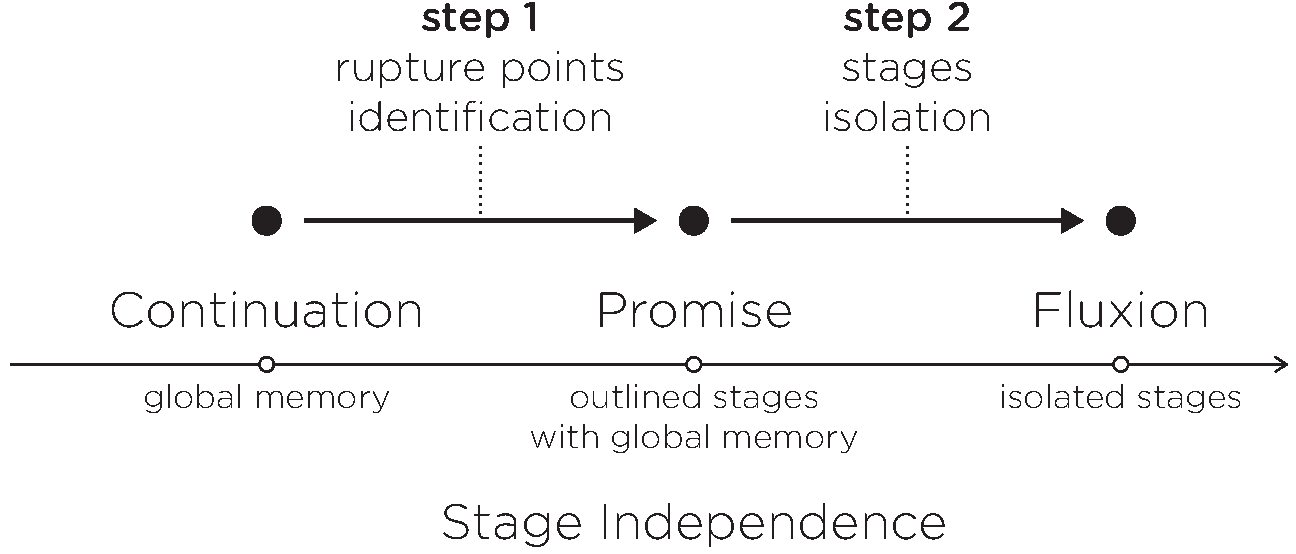
\includegraphics[width=0.7\textwidth]{../resources/roadmap.pdf}%
    \caption{Roadmap}%
    \label{fig:roadmap}%
  }%
\end{figure}

The first compiler focuses on the identification of simple chains of causality between continuations to transform these chains into Promises.
% the transformation from continuations to Promises.
% It focuses on the identification of the chains of causality in continuations.
However, promises are more expressive than the simple chaining of causal sequentiality.
% They force another control over the execution flow.
% According to the outcome of the operation, they call one function to continue the execution with the result, or another to handle errors.
% This conditional execution is indivisible from the Promise specification.
% Promises impose a convention on how to hand back the outcome of the deferred computation, while classic continuations leave this conditional execution to the developer.
Moreover, they impose a different convention than continuations on how to hand back the outcome and errors of the deferred computation.
This difference brings unnecessary complexity to the identification of chains.
To rule out this difference between continuations and Promises, before introducing the first compiler, section \ref{chapter5:due} introduces a simpler specification to Promise, called Due.

The second compiler detects all the chains of causality between continuations and encapsulate them in fluxions.
It isolates the fluxions when possible to allow the parallelism required for efficiency.
This second compilers is introduced in section \ref{chapter5:flx}.

\renewcommand{\glyph}{\iconfont{\XeTeXglyph287}}
\chapter{Implementations} \label{chapter5}
\minitoc
\eject
The transformation allowed by the equivalence from an event-driven program into a distributed network of fluxions is implemented incrementally into two compilers, as presented in figure \ref{fig:roadmap}.
Each compilers is divided into two steps, the identification of the rupture points separating the stages of the pipeline, and the isolation of these stages.
% This chapter presents the technical implementations of these two steps in the transformation from the event-driven execution model to the pipeline architecture
% , the transformation described in the previous chapter was implemented incrementally in two compilers.

\begin{figure}[h!]%
  \textfig{%
    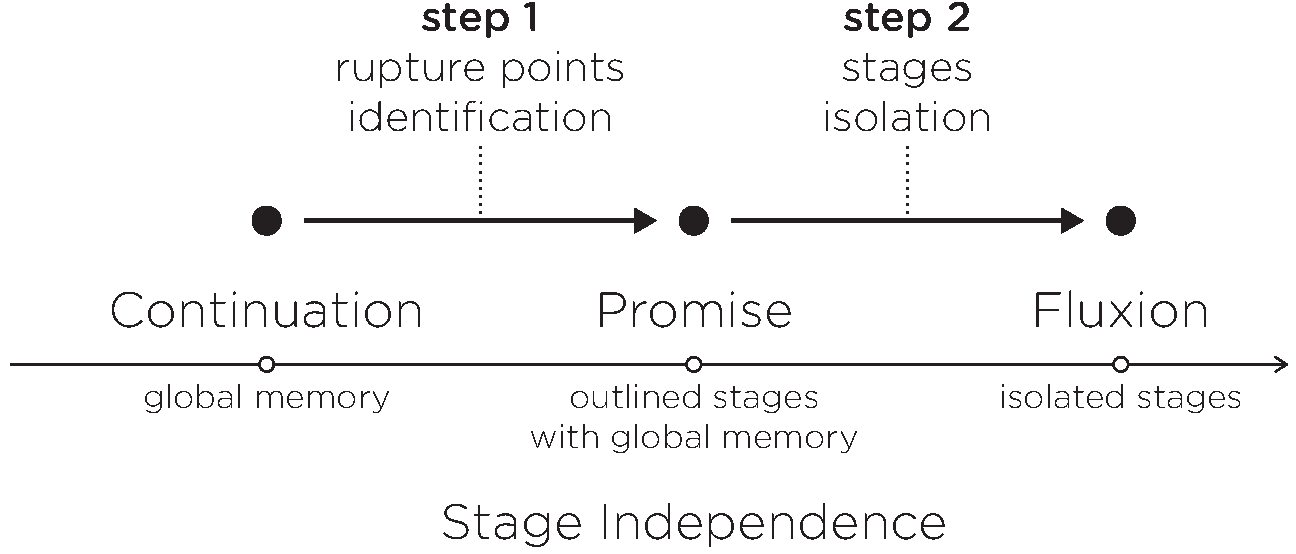
\includegraphics[width=0.7\textwidth]{../resources/roadmap.pdf}%
    \caption{Roadmap}%
    \label{fig:roadmap}%
  }%
\end{figure}

The first compiler focuses on the identification of simple chains of causality between continuations to transform these chains into Promises.
% the transformation from continuations to Promises.
% It focuses on the identification of the chains of causality in continuations.
However, promises are more expressive than the simple chaining of causal sequentiality.
% They force another control over the execution flow.
% According to the outcome of the operation, they call one function to continue the execution with the result, or another to handle errors.
% This conditional execution is indivisible from the Promise specification.
% Promises impose a convention on how to hand back the outcome of the deferred computation, while classic continuations leave this conditional execution to the developer.
Moreover, they impose a different convention than continuations on how to hand back the outcome and errors of the deferred computation.
This difference brings unnecessary complexity to the identification of chains.
To rule out this difference between continuations and Promises, before introducing the first compiler, section \ref{chapter5:due} introduces a simpler specification to Promise, called Due.

The second compiler detects all the chains of causality between continuations and encapsulate them in fluxions.
It isolates the fluxions when possible to allow the parallelism required for efficiency.
This second compilers is introduced in section \ref{chapter5:flx}.

\renewcommand{\glyph}{\iconfont{\XeTeXglyph287}}
\chapter{Implementations} \label{chapter5}
\minitoc
\eject
The transformation allowed by the equivalence from an event-driven program into a distributed network of fluxions is implemented incrementally into two compilers, as presented in figure \ref{fig:roadmap}.
Each compilers is divided into two steps, the identification of the rupture points separating the stages of the pipeline, and the isolation of these stages.
% This chapter presents the technical implementations of these two steps in the transformation from the event-driven execution model to the pipeline architecture
% , the transformation described in the previous chapter was implemented incrementally in two compilers.

\begin{figure}[h!]%
  \textfig{%
    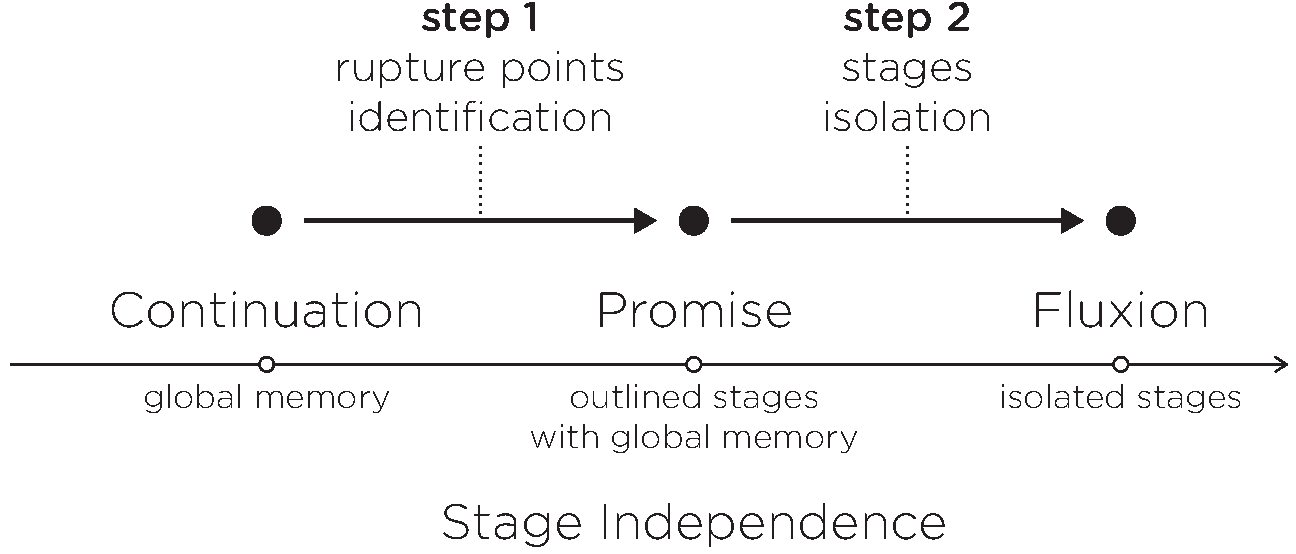
\includegraphics[width=0.7\textwidth]{../resources/roadmap.pdf}%
    \caption{Roadmap}%
    \label{fig:roadmap}%
  }%
\end{figure}

The first compiler focuses on the identification of simple chains of causality between continuations to transform these chains into Promises.
% the transformation from continuations to Promises.
% It focuses on the identification of the chains of causality in continuations.
However, promises are more expressive than the simple chaining of causal sequentiality.
% They force another control over the execution flow.
% According to the outcome of the operation, they call one function to continue the execution with the result, or another to handle errors.
% This conditional execution is indivisible from the Promise specification.
% Promises impose a convention on how to hand back the outcome of the deferred computation, while classic continuations leave this conditional execution to the developer.
Moreover, they impose a different convention than continuations on how to hand back the outcome and errors of the deferred computation.
This difference brings unnecessary complexity to the identification of chains.
To rule out this difference between continuations and Promises, before introducing the first compiler, section \ref{chapter5:due} introduces a simpler specification to Promise, called Due.

The second compiler detects all the chains of causality between continuations and encapsulate them in fluxions.
It isolates the fluxions when possible to allow the parallelism required for efficiency.
This second compilers is introduced in section \ref{chapter5:flx}.

\input{05-implementation/Due/main}
\input{05-implementation/Flx/main}
% \input{05-implementation/Evaluation}

\renewcommand{\glyph}{\iconfont{\XeTeXglyph287}}
\chapter{Implementations} \label{chapter5}
\minitoc
\eject
The transformation allowed by the equivalence from an event-driven program into a distributed network of fluxions is implemented incrementally into two compilers, as presented in figure \ref{fig:roadmap}.
Each compilers is divided into two steps, the identification of the rupture points separating the stages of the pipeline, and the isolation of these stages.
% This chapter presents the technical implementations of these two steps in the transformation from the event-driven execution model to the pipeline architecture
% , the transformation described in the previous chapter was implemented incrementally in two compilers.

\begin{figure}[h!]%
  \textfig{%
    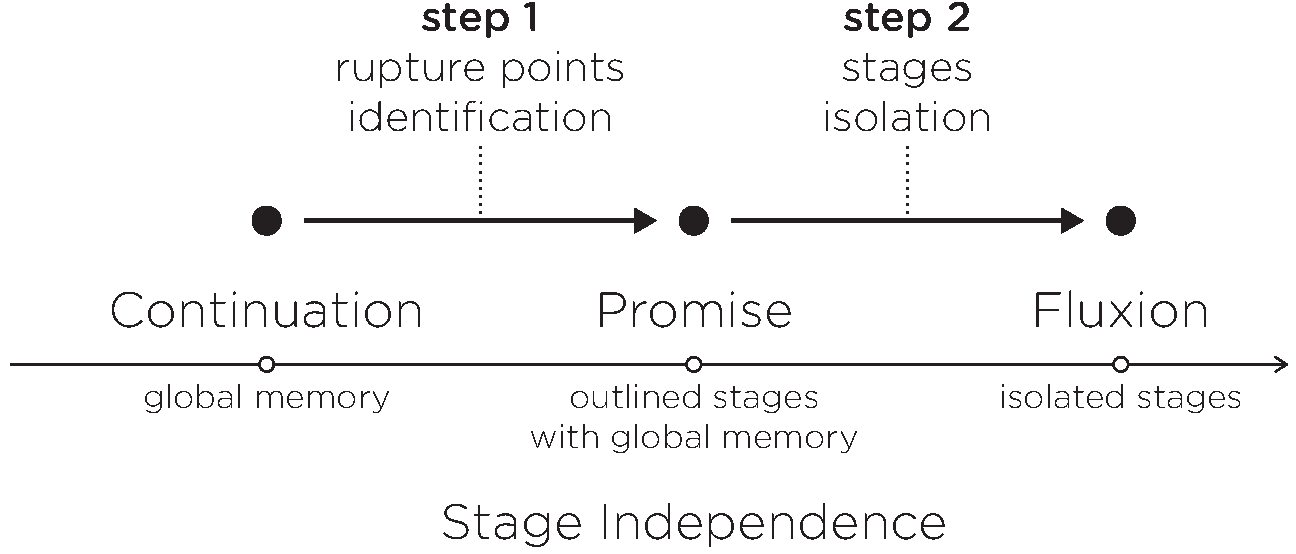
\includegraphics[width=0.7\textwidth]{../resources/roadmap.pdf}%
    \caption{Roadmap}%
    \label{fig:roadmap}%
  }%
\end{figure}

The first compiler focuses on the identification of simple chains of causality between continuations to transform these chains into Promises.
% the transformation from continuations to Promises.
% It focuses on the identification of the chains of causality in continuations.
However, promises are more expressive than the simple chaining of causal sequentiality.
% They force another control over the execution flow.
% According to the outcome of the operation, they call one function to continue the execution with the result, or another to handle errors.
% This conditional execution is indivisible from the Promise specification.
% Promises impose a convention on how to hand back the outcome of the deferred computation, while classic continuations leave this conditional execution to the developer.
Moreover, they impose a different convention than continuations on how to hand back the outcome and errors of the deferred computation.
This difference brings unnecessary complexity to the identification of chains.
To rule out this difference between continuations and Promises, before introducing the first compiler, section \ref{chapter5:due} introduces a simpler specification to Promise, called Due.

The second compiler detects all the chains of causality between continuations and encapsulate them in fluxions.
It isolates the fluxions when possible to allow the parallelism required for efficiency.
This second compilers is introduced in section \ref{chapter5:flx}.

\input{05-implementation/Due/main}
\input{05-implementation/Flx/main}
% \input{05-implementation/Evaluation}

% \subsection{Real test case} \label{chapter5:flx:evaluation}

The compiler is tested on a real application, gifsockets-server\ftnt{https://github.com/twolfson/gifsockets-server}.
This test proves the possibility for an application to be compiled into a network of independent parts.
It shows the current limitations of this isolation and the modifications needed on the application to circumvent them.

\begin{code}[js, caption={Simplified version of gifsockets-server},label={lst:gifsocket}]
var express = require('express'),
    app = express(),
    routes = require('gifsockets-middleware'), //@\label{lst:gifsocket:gif-mw}@
    getRawBody = require('raw-body');

function bodyParser(limit) { //@\label{lst:gifsocket:bodyParser}@
  return function saveBody(req, res, next) { //@\label{lst:gifsocket:saveBody}@
    getRawBody(req, { //@\label{lst:gifsocket:getRawBody}@
      expected: req.headers['content-length'],
      limit: limit
    }, function (err, buffer) { //@\label{lst:gifsocket:callback}@
      req.body = buffer;
      next(); //@\label{lst:gifsocket:next}@
    });
  };
}

app.post('/image/text', bodyParser(1 * 1024 * 1024), routes.writeTextToImages); //@\label{lst:gifsocket:app.post}@
app.listen(8000);
\end{code}

This application, simplified in listing \ref{lst:gifsocket}, is a real-time chat using gif-based communication channels.
It was selected from the evaluation set of the Due compiler because it is simple enough to illustrate this evaluation.
% \cite{Brodu2015}
%  from the \texttt{npm} registry because it depends on \texttt{express}, it is tested, working, and simple enough to illustrate this evaluation.
The server transforms the received text into a gif frame, and pushes it back to a never-ending gif to be displayed on the client.

On line \ref{lst:gifsocket:app.post}, the application registers two functions to process the requests received on the url \texttt{/image/text}.
The closure \texttt{saveBody}, line \ref{lst:gifsocket:saveBody}, returned by \texttt{bodyParser}, line \ref{lst:gifsocket:bodyParser}, and the method \texttt{routes.write\-Text\-To\-Images} from the external module \texttt{gifsockets-\-middleware}, line \ref{lst:gifsocket:gif-mw}.
The closure \texttt{saveBody} calls the asynchronous function \texttt{getRawBody} to get the request body.
Its callback handles the errors, and calls \texttt{next} to continue processing the request with the next function, \texttt{routes.write\-Text\-To\-Images}.

\subsubsection{Compilation} \label{chapter5:flx:evaluation:compilation}

% We compile this application with the compiler
The compilation result is in listing \ref{lst:flx-gifsocket}.
The function call \texttt{app.post}, line \ref{lst:gifsocket:app.post}, is a rupture point.
However, its callbacks, \texttt{bodyParser} and \texttt{routes.write\-Text\-To\-Images} are not declared \textit{in situ}.
They are evaluated as functions only at runtime.
As precised previously, the compiler discards these callbacks to avoid altering the semantic. % by moving or modifying their definition.
% For this reason, the compiler ignores this rupture point, to avoid interfering with the evaluation.

\begin{code}[flx, caption={Compilation result of gifsockets-server},label={lst:flx-gifsocket}]
flx main & express {req}
>> anonymous_1000 [req, next]
  var express = require('express'),
      app = express(),
      routes = require('gifsockets-middleware'), //@\label{lst:flx-gifsocket:gif-mw}@
      getRawBody = require('raw-body');

  function bodyParser(limit) { //@\label{lst:flx-gifsocket:bodyParser}@
    return function saveBody(req, res, next) { //@\label{lst:flx-gifsocket:saveBody}@
      getRawBody(req, { //@\label{lst:flx-gifsocket:getRawBody}@
        expected: req.headers['content-length'], //@\label{lst:flx-gifsocket:req.headers}@
        limit: limit
      }, >> anonymous_1000 [req, next]);
    };
  }

  app.post('/image/text', bodyParser(1 * 1024 * 1024), routes.writeTextToImages); //@\label{lst:flx-gifsocket:app.post}@
  app.listen(8000);

flx anonymous_1000
-> null
  function (err, buffer) { //@\label{lst:flx-gifsocket:callback}@
    req.body = buffer; //@\label{lst:flx-gifsocket:buffer}@
    next(); //@\label{lst:flx-gifsocket:next}@
  }
\end{code}

The compiler detects a rupture point : the function \texttt{get\-Raw\-Body} and its anonymous callback, line \ref{lst:gifsocket:callback}.
It encapsulates this callback in a fluxion named \texttt{anony\-mous\_\-1000}.
The callback is replaced with a stream placeholder to send the message stream to this downstream fluxion.
The variables \texttt{req} and \texttt{next} are appended to this message stream, to propagate their value from the \texttt{main} fluxion to the \texttt{anony\-mous\_\-1000} fluxion.

When \texttt{anony\-mous\_\-1000} is not isolated from the \texttt{main} fluxion, as if they belong to the same group, the compilation result works as expected.
The variables used in the fluxion, \texttt{req} and \texttt{next}, are still shared between the two fluxions.
In this situation fluxions are quite similar to Dues regarding memory shareing.
Our goal is to isolate the two fluxions, to be able to safely parallelize their executions.

\subsubsection{Isolation} \label{chapter5:flx:evaluation:isolation}

In listing \ref{lst:flx-gifsocket}, the fluxion \texttt{anony\-mous\_\-1000} modifies the object \texttt{req}, line \ref{lst:flx-gifsocket:buffer}, to store the text of the received request, and it calls \texttt{next} to continue the execution, line \ref{lst:flx-gifsocket:next}.
\texttt{req} is an alias to a memory location used in multiple palces in code.
Therefore, these operations produce side-effects that should propagate in the whole application, but the isolation prevents this propagation.
Isolating the fluxion \texttt{anony\-mous\_\-1000} produces runtime exceptions.
The next paragraph details how this situation is handled to allow the application to be parallelized.

\paragraph{Variable \texttt{req}}

The variable \texttt{req} is read in fluxion \texttt{main}, lines \ref{lst:flx-gifsocket:getRawBody} and \ref{lst:flx-gifsocket:req.headers}.
Then its property \texttt{body} is associated to \texttt{buffer} in fluxion \texttt{anony\-mous\_\-1000}, line \ref{lst:flx-gifsocket:buffer}.
The compiler is unable to identify the aliases of this variable. % further usages.
However, the side effect resulting from this association impacts a variable in the scope of the next callback, \texttt{routes.write\-Text\-To\-Images}.
In this test case, the application is modified manually to explicitly propagate this side-effect to the next callback through the function \texttt{next}.
The modifications of this function are explained further in the next paragraph.

\paragraph{Closure \texttt{next}}

The function \texttt{next} is a closure provided by the \texttt{express} \texttt{Router} to continue the execution with the next function to handle the client request.
Because it indirectly relies on the variable \texttt{req}, it is impossible to isolate its execution with the \texttt{anony\-mous\_\-1000} fluxion.
Instead, we modify \texttt{express}, so as to be compatible with the fluxional execution model.
We explain the modifications below.

\begin{code}[flx, caption={Simplified modification on the compiled result},label={lst:mflx-gifsocket}]
flx anonymous_1000
-> express_dispatcher
  function (err, buffer) { //@\label{lst:mflx-gifsocket:callback}@
    req.body = buffer; //@\label{lst:mflx-gifsocket:buffer}@
    next_placeholder(req, -> express_dispatcher); //@\label{lst:mflx-gifsocket:next-placeholder}@
  }

flx express_dispatcher & express {req} //@\label{lst:mflx-gifsocket:express-dispatcher}@
-> null
  function (modified_req) {
    merge(req, modified_req);
    next(); //@\label{lst:mflx-gifsocket:next}@
  }
\end{code}

In listing \ref{lst:gifsocket}, the function \texttt{next} is a continuation allowing the anonymous callback, line \ref{lst:gifsocket:callback}, to call the next function to handle the request.
To isolate the anonymous callback into \texttt{anonymous\_\-1000}, \texttt{next} is replaced by a rupture point.
This replacement is illustrated in listing \ref{lst:mflx-gifsocket}.
The \texttt{express} \texttt{Router} registers a fluxion named \texttt{express\_\-dispatcher}, line \ref{lst:mflx-gifsocket:express-dispatcher}, to continue the execution after the fluxion \texttt{anony\-mous\_\-1000}.
This fluxion is in the same group \texttt{express} as the \texttt{main} fluxion, hence it has access to the original variable \texttt{req}, and to the original function \texttt{next}.
The call to the original \texttt{next} function is replaced by a placeholder to push the stream to the fluxion \texttt{express\_\-dispatcher}, line \ref{lst:mflx-gifsocket:next-placeholder}.
The fluxion \texttt{express\_\-dispatcher} receives the stream from the upstream fluxion \texttt{anony\-mous\_\-1000}, merges back the modification in the variable \texttt{req} to propagate the side effects, and finally calls the original function \texttt{next} to continue the execution, line \ref{lst:mflx-gifsocket:next}.

After the modifications detailed above, the server works as expected.
The isolated fluxion correctly receives, and returns its serialized messages.
The client successfully receives a gif frame containing the text.



\subsection{Limitations}

The static analysis used for this compiler presents some limitations.
It is unable to analyze code with dynamic behaviors.
Higher-order programming leads to more productivity partly beacuse it rely on such dynamic behavior to extend expressivity.
Precisely, it allows more levels of indirections.

\subsubsection{Levels of Indirections}

The indirection is an abstraction between the value, and its manipulation.
In listing \ref{lst:indirection}, the variables \texttt{a} and \texttt{b} point both to the same memory object.
The function \texttt{fn} introduces a level of indirection between the real object \texttt{a} and its manipulation handle, \texttt{b};
% Actually, the variable \texttt{a} already introduces a level of indirection between the real object and the handle \texttt{a}.

\begin{code}[js,
  caption={One level of Indirection},
  label={lst:indirection}]
var a = {
      // an object;
    };

fn(b) {
  // modify b;
}

fn(a);
\end{code}

\subsubsection{Uncertainties}

The indirection is trivial to resolve in listing \ref{lst:indirection}.
It only needs to have access to the definition of \texttt{a} and of \texttt{fn}.
%A very simple static analysis could resolve it.
However, in listing \ref{lst:indirections}, the array \texttt{handlers} introduces a new level of indirection.
The static analysis now needs to have access to the definition of \texttt{i} and of the \texttt{handlers}.
If this definition is provided by an external input, it is not available statically, hence, it adds an uncertainty during the analysis. 

\begin{code}[js,
  caption={Two levels of indirection},
  label={lst:indirections}]
var a = {
      // an object;
    },
    handlers = [
      // definition of fn handlers;
    ],
    i = ?;

handlers[i](a);
handlers[i+1](a);
\end{code}

These examples are extremely simplified.
A real application contains enough indirections for the static analysis to be overwhelmed by uncertainties, and to be unable to resolve the variables.
If a variable is left unresolved, it is impossible to assure its scope and its aliases.
Therefore, the compiler is unable to isolate it into a fluxion, or to distribute its modification by messages.

Moreover, it leads the compiler to ignore the rupture points not defined \textit{in situ}, because their modifications could impact the semantic.
The reason for this precaution, is that the compiler is unable to assure where the function is used, and the scope of its variables.
Therefore, it is unable to assure that the modification will conserve the semantic.

\subsubsection{Dynamic Resolution}

In a web application, this variable \texttt{i} might be part of the user request, which is available only at runtime.
It eventually introduces an uncertainty.

This dynamic resolution of variables is precisely what increase expressiveness.
Trying to resolve them statically is equivalent to restrict expressiveness.
No static analysis can overstep these limitations.
Only a dynamic analysis could analysis the resolved indirections during run time to overstep these limitations correctly.




\renewcommand{\glyph}{\iconfont{\XeTeXglyph287}}
\chapter{Implementations} \label{chapter5}
\minitoc
\eject
The transformation allowed by the equivalence from an event-driven program into a distributed network of fluxions is implemented incrementally into two compilers, as presented in figure \ref{fig:roadmap}.
Each compilers is divided into two steps, the identification of the rupture points separating the stages of the pipeline, and the isolation of these stages.
% This chapter presents the technical implementations of these two steps in the transformation from the event-driven execution model to the pipeline architecture
% , the transformation described in the previous chapter was implemented incrementally in two compilers.

\begin{figure}[h!]%
  \textfig{%
    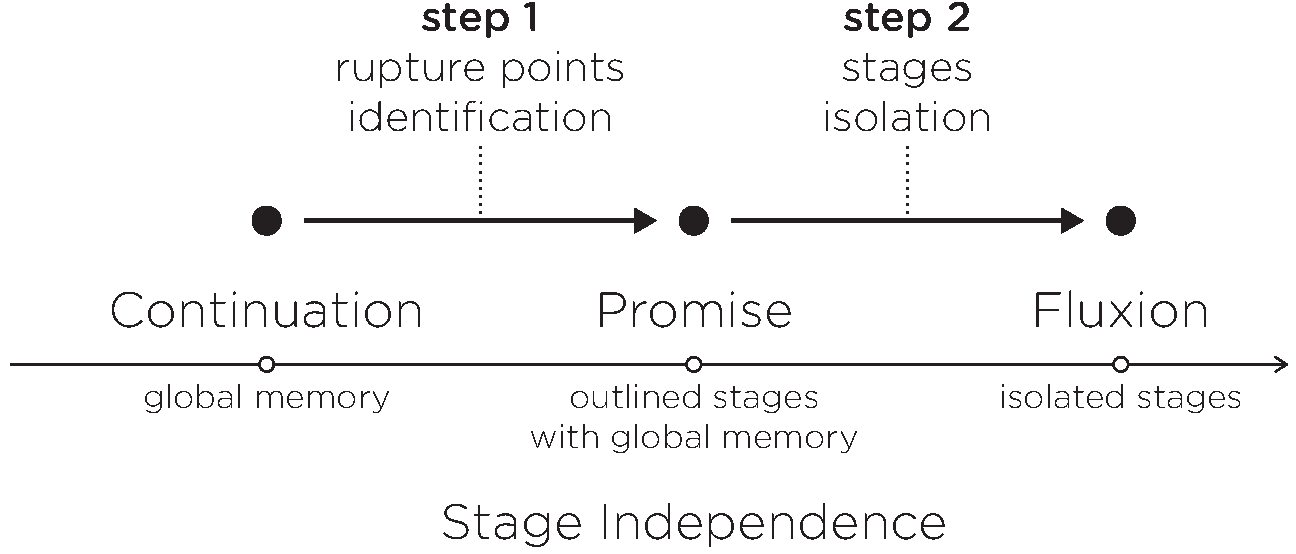
\includegraphics[width=0.7\textwidth]{../resources/roadmap.pdf}%
    \caption{Roadmap}%
    \label{fig:roadmap}%
  }%
\end{figure}

The first compiler focuses on the identification of simple chains of causality between continuations to transform these chains into Promises.
% the transformation from continuations to Promises.
% It focuses on the identification of the chains of causality in continuations.
However, promises are more expressive than the simple chaining of causal sequentiality.
% They force another control over the execution flow.
% According to the outcome of the operation, they call one function to continue the execution with the result, or another to handle errors.
% This conditional execution is indivisible from the Promise specification.
% Promises impose a convention on how to hand back the outcome of the deferred computation, while classic continuations leave this conditional execution to the developer.
Moreover, they impose a different convention than continuations on how to hand back the outcome and errors of the deferred computation.
This difference brings unnecessary complexity to the identification of chains.
To rule out this difference between continuations and Promises, before introducing the first compiler, section \ref{chapter5:due} introduces a simpler specification to Promise, called Due.

The second compiler detects all the chains of causality between continuations and encapsulate them in fluxions.
It isolates the fluxions when possible to allow the parallelism required for efficiency.
This second compilers is introduced in section \ref{chapter5:flx}.

\renewcommand{\glyph}{\iconfont{\XeTeXglyph287}}
\chapter{Implementations} \label{chapter5}
\minitoc
\eject
The transformation allowed by the equivalence from an event-driven program into a distributed network of fluxions is implemented incrementally into two compilers, as presented in figure \ref{fig:roadmap}.
Each compilers is divided into two steps, the identification of the rupture points separating the stages of the pipeline, and the isolation of these stages.
% This chapter presents the technical implementations of these two steps in the transformation from the event-driven execution model to the pipeline architecture
% , the transformation described in the previous chapter was implemented incrementally in two compilers.

\begin{figure}[h!]%
  \textfig{%
    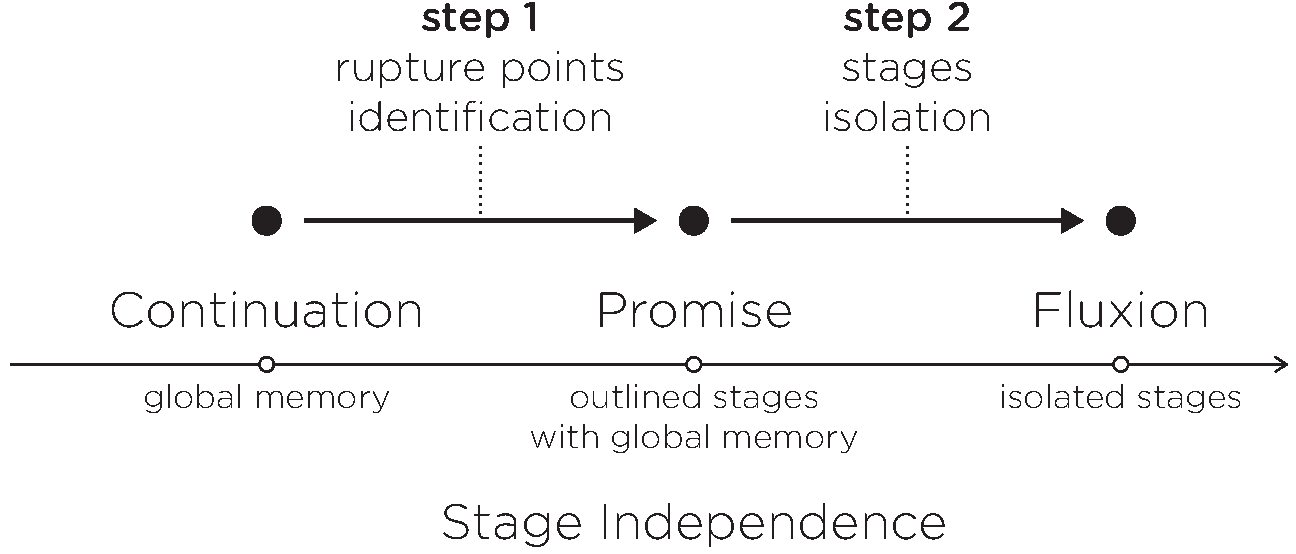
\includegraphics[width=0.7\textwidth]{../resources/roadmap.pdf}%
    \caption{Roadmap}%
    \label{fig:roadmap}%
  }%
\end{figure}

The first compiler focuses on the identification of simple chains of causality between continuations to transform these chains into Promises.
% the transformation from continuations to Promises.
% It focuses on the identification of the chains of causality in continuations.
However, promises are more expressive than the simple chaining of causal sequentiality.
% They force another control over the execution flow.
% According to the outcome of the operation, they call one function to continue the execution with the result, or another to handle errors.
% This conditional execution is indivisible from the Promise specification.
% Promises impose a convention on how to hand back the outcome of the deferred computation, while classic continuations leave this conditional execution to the developer.
Moreover, they impose a different convention than continuations on how to hand back the outcome and errors of the deferred computation.
This difference brings unnecessary complexity to the identification of chains.
To rule out this difference between continuations and Promises, before introducing the first compiler, section \ref{chapter5:due} introduces a simpler specification to Promise, called Due.

The second compiler detects all the chains of causality between continuations and encapsulate them in fluxions.
It isolates the fluxions when possible to allow the parallelism required for efficiency.
This second compilers is introduced in section \ref{chapter5:flx}.

\input{05-implementation/Due/main}
\input{05-implementation/Flx/main}
% \input{05-implementation/Evaluation}

\renewcommand{\glyph}{\iconfont{\XeTeXglyph287}}
\chapter{Implementations} \label{chapter5}
\minitoc
\eject
The transformation allowed by the equivalence from an event-driven program into a distributed network of fluxions is implemented incrementally into two compilers, as presented in figure \ref{fig:roadmap}.
Each compilers is divided into two steps, the identification of the rupture points separating the stages of the pipeline, and the isolation of these stages.
% This chapter presents the technical implementations of these two steps in the transformation from the event-driven execution model to the pipeline architecture
% , the transformation described in the previous chapter was implemented incrementally in two compilers.

\begin{figure}[h!]%
  \textfig{%
    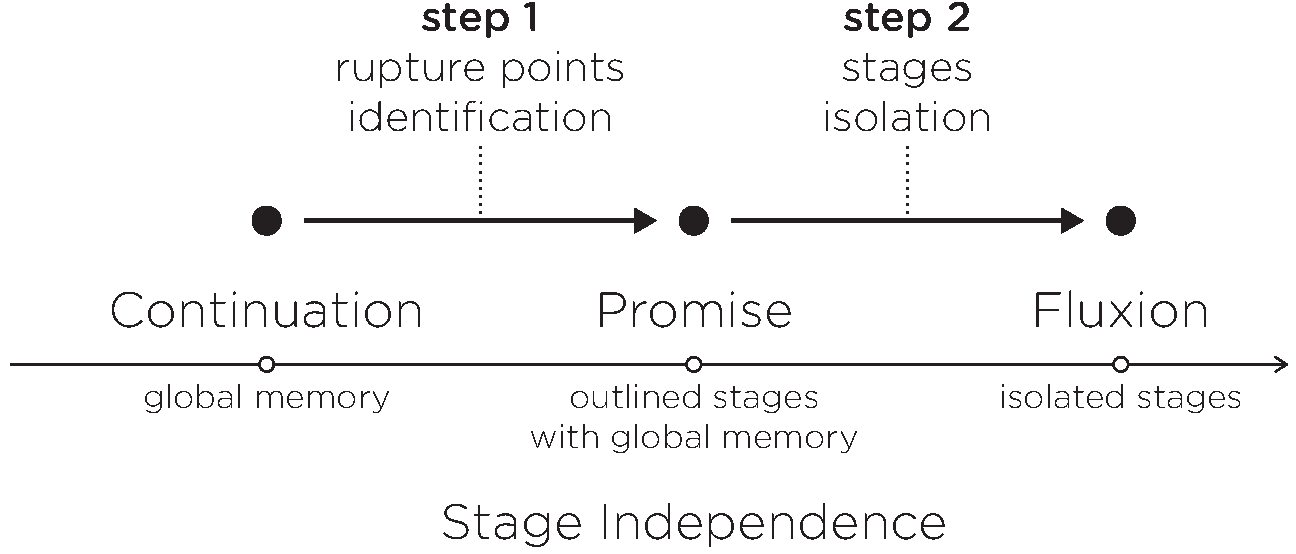
\includegraphics[width=0.7\textwidth]{../resources/roadmap.pdf}%
    \caption{Roadmap}%
    \label{fig:roadmap}%
  }%
\end{figure}

The first compiler focuses on the identification of simple chains of causality between continuations to transform these chains into Promises.
% the transformation from continuations to Promises.
% It focuses on the identification of the chains of causality in continuations.
However, promises are more expressive than the simple chaining of causal sequentiality.
% They force another control over the execution flow.
% According to the outcome of the operation, they call one function to continue the execution with the result, or another to handle errors.
% This conditional execution is indivisible from the Promise specification.
% Promises impose a convention on how to hand back the outcome of the deferred computation, while classic continuations leave this conditional execution to the developer.
Moreover, they impose a different convention than continuations on how to hand back the outcome and errors of the deferred computation.
This difference brings unnecessary complexity to the identification of chains.
To rule out this difference between continuations and Promises, before introducing the first compiler, section \ref{chapter5:due} introduces a simpler specification to Promise, called Due.

The second compiler detects all the chains of causality between continuations and encapsulate them in fluxions.
It isolates the fluxions when possible to allow the parallelism required for efficiency.
This second compilers is introduced in section \ref{chapter5:flx}.

\input{05-implementation/Due/main}
\input{05-implementation/Flx/main}
% \input{05-implementation/Evaluation}

% \subsection{Real test case} \label{chapter5:flx:evaluation}

The compiler is tested on a real application, gifsockets-server\ftnt{https://github.com/twolfson/gifsockets-server}.
This test proves the possibility for an application to be compiled into a network of independent parts.
It shows the current limitations of this isolation and the modifications needed on the application to circumvent them.

\begin{code}[js, caption={Simplified version of gifsockets-server},label={lst:gifsocket}]
var express = require('express'),
    app = express(),
    routes = require('gifsockets-middleware'), //@\label{lst:gifsocket:gif-mw}@
    getRawBody = require('raw-body');

function bodyParser(limit) { //@\label{lst:gifsocket:bodyParser}@
  return function saveBody(req, res, next) { //@\label{lst:gifsocket:saveBody}@
    getRawBody(req, { //@\label{lst:gifsocket:getRawBody}@
      expected: req.headers['content-length'],
      limit: limit
    }, function (err, buffer) { //@\label{lst:gifsocket:callback}@
      req.body = buffer;
      next(); //@\label{lst:gifsocket:next}@
    });
  };
}

app.post('/image/text', bodyParser(1 * 1024 * 1024), routes.writeTextToImages); //@\label{lst:gifsocket:app.post}@
app.listen(8000);
\end{code}

This application, simplified in listing \ref{lst:gifsocket}, is a real-time chat using gif-based communication channels.
It was selected from the evaluation set of the Due compiler because it is simple enough to illustrate this evaluation.
% \cite{Brodu2015}
%  from the \texttt{npm} registry because it depends on \texttt{express}, it is tested, working, and simple enough to illustrate this evaluation.
The server transforms the received text into a gif frame, and pushes it back to a never-ending gif to be displayed on the client.

On line \ref{lst:gifsocket:app.post}, the application registers two functions to process the requests received on the url \texttt{/image/text}.
The closure \texttt{saveBody}, line \ref{lst:gifsocket:saveBody}, returned by \texttt{bodyParser}, line \ref{lst:gifsocket:bodyParser}, and the method \texttt{routes.write\-Text\-To\-Images} from the external module \texttt{gifsockets-\-middleware}, line \ref{lst:gifsocket:gif-mw}.
The closure \texttt{saveBody} calls the asynchronous function \texttt{getRawBody} to get the request body.
Its callback handles the errors, and calls \texttt{next} to continue processing the request with the next function, \texttt{routes.write\-Text\-To\-Images}.

\subsubsection{Compilation} \label{chapter5:flx:evaluation:compilation}

% We compile this application with the compiler
The compilation result is in listing \ref{lst:flx-gifsocket}.
The function call \texttt{app.post}, line \ref{lst:gifsocket:app.post}, is a rupture point.
However, its callbacks, \texttt{bodyParser} and \texttt{routes.write\-Text\-To\-Images} are not declared \textit{in situ}.
They are evaluated as functions only at runtime.
As precised previously, the compiler discards these callbacks to avoid altering the semantic. % by moving or modifying their definition.
% For this reason, the compiler ignores this rupture point, to avoid interfering with the evaluation.

\begin{code}[flx, caption={Compilation result of gifsockets-server},label={lst:flx-gifsocket}]
flx main & express {req}
>> anonymous_1000 [req, next]
  var express = require('express'),
      app = express(),
      routes = require('gifsockets-middleware'), //@\label{lst:flx-gifsocket:gif-mw}@
      getRawBody = require('raw-body');

  function bodyParser(limit) { //@\label{lst:flx-gifsocket:bodyParser}@
    return function saveBody(req, res, next) { //@\label{lst:flx-gifsocket:saveBody}@
      getRawBody(req, { //@\label{lst:flx-gifsocket:getRawBody}@
        expected: req.headers['content-length'], //@\label{lst:flx-gifsocket:req.headers}@
        limit: limit
      }, >> anonymous_1000 [req, next]);
    };
  }

  app.post('/image/text', bodyParser(1 * 1024 * 1024), routes.writeTextToImages); //@\label{lst:flx-gifsocket:app.post}@
  app.listen(8000);

flx anonymous_1000
-> null
  function (err, buffer) { //@\label{lst:flx-gifsocket:callback}@
    req.body = buffer; //@\label{lst:flx-gifsocket:buffer}@
    next(); //@\label{lst:flx-gifsocket:next}@
  }
\end{code}

The compiler detects a rupture point : the function \texttt{get\-Raw\-Body} and its anonymous callback, line \ref{lst:gifsocket:callback}.
It encapsulates this callback in a fluxion named \texttt{anony\-mous\_\-1000}.
The callback is replaced with a stream placeholder to send the message stream to this downstream fluxion.
The variables \texttt{req} and \texttt{next} are appended to this message stream, to propagate their value from the \texttt{main} fluxion to the \texttt{anony\-mous\_\-1000} fluxion.

When \texttt{anony\-mous\_\-1000} is not isolated from the \texttt{main} fluxion, as if they belong to the same group, the compilation result works as expected.
The variables used in the fluxion, \texttt{req} and \texttt{next}, are still shared between the two fluxions.
In this situation fluxions are quite similar to Dues regarding memory shareing.
Our goal is to isolate the two fluxions, to be able to safely parallelize their executions.

\subsubsection{Isolation} \label{chapter5:flx:evaluation:isolation}

In listing \ref{lst:flx-gifsocket}, the fluxion \texttt{anony\-mous\_\-1000} modifies the object \texttt{req}, line \ref{lst:flx-gifsocket:buffer}, to store the text of the received request, and it calls \texttt{next} to continue the execution, line \ref{lst:flx-gifsocket:next}.
\texttt{req} is an alias to a memory location used in multiple palces in code.
Therefore, these operations produce side-effects that should propagate in the whole application, but the isolation prevents this propagation.
Isolating the fluxion \texttt{anony\-mous\_\-1000} produces runtime exceptions.
The next paragraph details how this situation is handled to allow the application to be parallelized.

\paragraph{Variable \texttt{req}}

The variable \texttt{req} is read in fluxion \texttt{main}, lines \ref{lst:flx-gifsocket:getRawBody} and \ref{lst:flx-gifsocket:req.headers}.
Then its property \texttt{body} is associated to \texttt{buffer} in fluxion \texttt{anony\-mous\_\-1000}, line \ref{lst:flx-gifsocket:buffer}.
The compiler is unable to identify the aliases of this variable. % further usages.
However, the side effect resulting from this association impacts a variable in the scope of the next callback, \texttt{routes.write\-Text\-To\-Images}.
In this test case, the application is modified manually to explicitly propagate this side-effect to the next callback through the function \texttt{next}.
The modifications of this function are explained further in the next paragraph.

\paragraph{Closure \texttt{next}}

The function \texttt{next} is a closure provided by the \texttt{express} \texttt{Router} to continue the execution with the next function to handle the client request.
Because it indirectly relies on the variable \texttt{req}, it is impossible to isolate its execution with the \texttt{anony\-mous\_\-1000} fluxion.
Instead, we modify \texttt{express}, so as to be compatible with the fluxional execution model.
We explain the modifications below.

\begin{code}[flx, caption={Simplified modification on the compiled result},label={lst:mflx-gifsocket}]
flx anonymous_1000
-> express_dispatcher
  function (err, buffer) { //@\label{lst:mflx-gifsocket:callback}@
    req.body = buffer; //@\label{lst:mflx-gifsocket:buffer}@
    next_placeholder(req, -> express_dispatcher); //@\label{lst:mflx-gifsocket:next-placeholder}@
  }

flx express_dispatcher & express {req} //@\label{lst:mflx-gifsocket:express-dispatcher}@
-> null
  function (modified_req) {
    merge(req, modified_req);
    next(); //@\label{lst:mflx-gifsocket:next}@
  }
\end{code}

In listing \ref{lst:gifsocket}, the function \texttt{next} is a continuation allowing the anonymous callback, line \ref{lst:gifsocket:callback}, to call the next function to handle the request.
To isolate the anonymous callback into \texttt{anonymous\_\-1000}, \texttt{next} is replaced by a rupture point.
This replacement is illustrated in listing \ref{lst:mflx-gifsocket}.
The \texttt{express} \texttt{Router} registers a fluxion named \texttt{express\_\-dispatcher}, line \ref{lst:mflx-gifsocket:express-dispatcher}, to continue the execution after the fluxion \texttt{anony\-mous\_\-1000}.
This fluxion is in the same group \texttt{express} as the \texttt{main} fluxion, hence it has access to the original variable \texttt{req}, and to the original function \texttt{next}.
The call to the original \texttt{next} function is replaced by a placeholder to push the stream to the fluxion \texttt{express\_\-dispatcher}, line \ref{lst:mflx-gifsocket:next-placeholder}.
The fluxion \texttt{express\_\-dispatcher} receives the stream from the upstream fluxion \texttt{anony\-mous\_\-1000}, merges back the modification in the variable \texttt{req} to propagate the side effects, and finally calls the original function \texttt{next} to continue the execution, line \ref{lst:mflx-gifsocket:next}.

After the modifications detailed above, the server works as expected.
The isolated fluxion correctly receives, and returns its serialized messages.
The client successfully receives a gif frame containing the text.



\subsection{Limitations}

The static analysis used for this compiler presents some limitations.
It is unable to analyze code with dynamic behaviors.
Higher-order programming leads to more productivity partly beacuse it rely on such dynamic behavior to extend expressivity.
Precisely, it allows more levels of indirections.

\subsubsection{Levels of Indirections}

The indirection is an abstraction between the value, and its manipulation.
In listing \ref{lst:indirection}, the variables \texttt{a} and \texttt{b} point both to the same memory object.
The function \texttt{fn} introduces a level of indirection between the real object \texttt{a} and its manipulation handle, \texttt{b};
% Actually, the variable \texttt{a} already introduces a level of indirection between the real object and the handle \texttt{a}.

\begin{code}[js,
  caption={One level of Indirection},
  label={lst:indirection}]
var a = {
      // an object;
    };

fn(b) {
  // modify b;
}

fn(a);
\end{code}

\subsubsection{Uncertainties}

The indirection is trivial to resolve in listing \ref{lst:indirection}.
It only needs to have access to the definition of \texttt{a} and of \texttt{fn}.
%A very simple static analysis could resolve it.
However, in listing \ref{lst:indirections}, the array \texttt{handlers} introduces a new level of indirection.
The static analysis now needs to have access to the definition of \texttt{i} and of the \texttt{handlers}.
If this definition is provided by an external input, it is not available statically, hence, it adds an uncertainty during the analysis. 

\begin{code}[js,
  caption={Two levels of indirection},
  label={lst:indirections}]
var a = {
      // an object;
    },
    handlers = [
      // definition of fn handlers;
    ],
    i = ?;

handlers[i](a);
handlers[i+1](a);
\end{code}

These examples are extremely simplified.
A real application contains enough indirections for the static analysis to be overwhelmed by uncertainties, and to be unable to resolve the variables.
If a variable is left unresolved, it is impossible to assure its scope and its aliases.
Therefore, the compiler is unable to isolate it into a fluxion, or to distribute its modification by messages.

Moreover, it leads the compiler to ignore the rupture points not defined \textit{in situ}, because their modifications could impact the semantic.
The reason for this precaution, is that the compiler is unable to assure where the function is used, and the scope of its variables.
Therefore, it is unable to assure that the modification will conserve the semantic.

\subsubsection{Dynamic Resolution}

In a web application, this variable \texttt{i} might be part of the user request, which is available only at runtime.
It eventually introduces an uncertainty.

This dynamic resolution of variables is precisely what increase expressiveness.
Trying to resolve them statically is equivalent to restrict expressiveness.
No static analysis can overstep these limitations.
Only a dynamic analysis could analysis the resolved indirections during run time to overstep these limitations correctly.




% \subsection{Real test case} \label{chapter5:flx:evaluation}

The compiler is tested on a real application, gifsockets-server\ftnt{https://github.com/twolfson/gifsockets-server}.
This test proves the possibility for an application to be compiled into a network of independent parts.
It shows the current limitations of this isolation and the modifications needed on the application to circumvent them.

\begin{code}[js, caption={Simplified version of gifsockets-server},label={lst:gifsocket}]
var express = require('express'),
    app = express(),
    routes = require('gifsockets-middleware'), //@\label{lst:gifsocket:gif-mw}@
    getRawBody = require('raw-body');

function bodyParser(limit) { //@\label{lst:gifsocket:bodyParser}@
  return function saveBody(req, res, next) { //@\label{lst:gifsocket:saveBody}@
    getRawBody(req, { //@\label{lst:gifsocket:getRawBody}@
      expected: req.headers['content-length'],
      limit: limit
    }, function (err, buffer) { //@\label{lst:gifsocket:callback}@
      req.body = buffer;
      next(); //@\label{lst:gifsocket:next}@
    });
  };
}

app.post('/image/text', bodyParser(1 * 1024 * 1024), routes.writeTextToImages); //@\label{lst:gifsocket:app.post}@
app.listen(8000);
\end{code}

This application, simplified in listing \ref{lst:gifsocket}, is a real-time chat using gif-based communication channels.
It was selected from the evaluation set of the Due compiler because it is simple enough to illustrate this evaluation.
% \cite{Brodu2015}
%  from the \texttt{npm} registry because it depends on \texttt{express}, it is tested, working, and simple enough to illustrate this evaluation.
The server transforms the received text into a gif frame, and pushes it back to a never-ending gif to be displayed on the client.

On line \ref{lst:gifsocket:app.post}, the application registers two functions to process the requests received on the url \texttt{/image/text}.
The closure \texttt{saveBody}, line \ref{lst:gifsocket:saveBody}, returned by \texttt{bodyParser}, line \ref{lst:gifsocket:bodyParser}, and the method \texttt{routes.write\-Text\-To\-Images} from the external module \texttt{gifsockets-\-middleware}, line \ref{lst:gifsocket:gif-mw}.
The closure \texttt{saveBody} calls the asynchronous function \texttt{getRawBody} to get the request body.
Its callback handles the errors, and calls \texttt{next} to continue processing the request with the next function, \texttt{routes.write\-Text\-To\-Images}.

\subsubsection{Compilation} \label{chapter5:flx:evaluation:compilation}

% We compile this application with the compiler
The compilation result is in listing \ref{lst:flx-gifsocket}.
The function call \texttt{app.post}, line \ref{lst:gifsocket:app.post}, is a rupture point.
However, its callbacks, \texttt{bodyParser} and \texttt{routes.write\-Text\-To\-Images} are not declared \textit{in situ}.
They are evaluated as functions only at runtime.
As precised previously, the compiler discards these callbacks to avoid altering the semantic. % by moving or modifying their definition.
% For this reason, the compiler ignores this rupture point, to avoid interfering with the evaluation.

\begin{code}[flx, caption={Compilation result of gifsockets-server},label={lst:flx-gifsocket}]
flx main & express {req}
>> anonymous_1000 [req, next]
  var express = require('express'),
      app = express(),
      routes = require('gifsockets-middleware'), //@\label{lst:flx-gifsocket:gif-mw}@
      getRawBody = require('raw-body');

  function bodyParser(limit) { //@\label{lst:flx-gifsocket:bodyParser}@
    return function saveBody(req, res, next) { //@\label{lst:flx-gifsocket:saveBody}@
      getRawBody(req, { //@\label{lst:flx-gifsocket:getRawBody}@
        expected: req.headers['content-length'], //@\label{lst:flx-gifsocket:req.headers}@
        limit: limit
      }, >> anonymous_1000 [req, next]);
    };
  }

  app.post('/image/text', bodyParser(1 * 1024 * 1024), routes.writeTextToImages); //@\label{lst:flx-gifsocket:app.post}@
  app.listen(8000);

flx anonymous_1000
-> null
  function (err, buffer) { //@\label{lst:flx-gifsocket:callback}@
    req.body = buffer; //@\label{lst:flx-gifsocket:buffer}@
    next(); //@\label{lst:flx-gifsocket:next}@
  }
\end{code}

The compiler detects a rupture point : the function \texttt{get\-Raw\-Body} and its anonymous callback, line \ref{lst:gifsocket:callback}.
It encapsulates this callback in a fluxion named \texttt{anony\-mous\_\-1000}.
The callback is replaced with a stream placeholder to send the message stream to this downstream fluxion.
The variables \texttt{req} and \texttt{next} are appended to this message stream, to propagate their value from the \texttt{main} fluxion to the \texttt{anony\-mous\_\-1000} fluxion.

When \texttt{anony\-mous\_\-1000} is not isolated from the \texttt{main} fluxion, as if they belong to the same group, the compilation result works as expected.
The variables used in the fluxion, \texttt{req} and \texttt{next}, are still shared between the two fluxions.
In this situation fluxions are quite similar to Dues regarding memory shareing.
Our goal is to isolate the two fluxions, to be able to safely parallelize their executions.

\subsubsection{Isolation} \label{chapter5:flx:evaluation:isolation}

In listing \ref{lst:flx-gifsocket}, the fluxion \texttt{anony\-mous\_\-1000} modifies the object \texttt{req}, line \ref{lst:flx-gifsocket:buffer}, to store the text of the received request, and it calls \texttt{next} to continue the execution, line \ref{lst:flx-gifsocket:next}.
\texttt{req} is an alias to a memory location used in multiple palces in code.
Therefore, these operations produce side-effects that should propagate in the whole application, but the isolation prevents this propagation.
Isolating the fluxion \texttt{anony\-mous\_\-1000} produces runtime exceptions.
The next paragraph details how this situation is handled to allow the application to be parallelized.

\paragraph{Variable \texttt{req}}

The variable \texttt{req} is read in fluxion \texttt{main}, lines \ref{lst:flx-gifsocket:getRawBody} and \ref{lst:flx-gifsocket:req.headers}.
Then its property \texttt{body} is associated to \texttt{buffer} in fluxion \texttt{anony\-mous\_\-1000}, line \ref{lst:flx-gifsocket:buffer}.
The compiler is unable to identify the aliases of this variable. % further usages.
However, the side effect resulting from this association impacts a variable in the scope of the next callback, \texttt{routes.write\-Text\-To\-Images}.
In this test case, the application is modified manually to explicitly propagate this side-effect to the next callback through the function \texttt{next}.
The modifications of this function are explained further in the next paragraph.

\paragraph{Closure \texttt{next}}

The function \texttt{next} is a closure provided by the \texttt{express} \texttt{Router} to continue the execution with the next function to handle the client request.
Because it indirectly relies on the variable \texttt{req}, it is impossible to isolate its execution with the \texttt{anony\-mous\_\-1000} fluxion.
Instead, we modify \texttt{express}, so as to be compatible with the fluxional execution model.
We explain the modifications below.

\begin{code}[flx, caption={Simplified modification on the compiled result},label={lst:mflx-gifsocket}]
flx anonymous_1000
-> express_dispatcher
  function (err, buffer) { //@\label{lst:mflx-gifsocket:callback}@
    req.body = buffer; //@\label{lst:mflx-gifsocket:buffer}@
    next_placeholder(req, -> express_dispatcher); //@\label{lst:mflx-gifsocket:next-placeholder}@
  }

flx express_dispatcher & express {req} //@\label{lst:mflx-gifsocket:express-dispatcher}@
-> null
  function (modified_req) {
    merge(req, modified_req);
    next(); //@\label{lst:mflx-gifsocket:next}@
  }
\end{code}

In listing \ref{lst:gifsocket}, the function \texttt{next} is a continuation allowing the anonymous callback, line \ref{lst:gifsocket:callback}, to call the next function to handle the request.
To isolate the anonymous callback into \texttt{anonymous\_\-1000}, \texttt{next} is replaced by a rupture point.
This replacement is illustrated in listing \ref{lst:mflx-gifsocket}.
The \texttt{express} \texttt{Router} registers a fluxion named \texttt{express\_\-dispatcher}, line \ref{lst:mflx-gifsocket:express-dispatcher}, to continue the execution after the fluxion \texttt{anony\-mous\_\-1000}.
This fluxion is in the same group \texttt{express} as the \texttt{main} fluxion, hence it has access to the original variable \texttt{req}, and to the original function \texttt{next}.
The call to the original \texttt{next} function is replaced by a placeholder to push the stream to the fluxion \texttt{express\_\-dispatcher}, line \ref{lst:mflx-gifsocket:next-placeholder}.
The fluxion \texttt{express\_\-dispatcher} receives the stream from the upstream fluxion \texttt{anony\-mous\_\-1000}, merges back the modification in the variable \texttt{req} to propagate the side effects, and finally calls the original function \texttt{next} to continue the execution, line \ref{lst:mflx-gifsocket:next}.

After the modifications detailed above, the server works as expected.
The isolated fluxion correctly receives, and returns its serialized messages.
The client successfully receives a gif frame containing the text.



\subsection{Limitations}

The static analysis used for this compiler presents some limitations.
It is unable to analyze code with dynamic behaviors.
Higher-order programming leads to more productivity partly beacuse it rely on such dynamic behavior to extend expressivity.
Precisely, it allows more levels of indirections.

\subsubsection{Levels of Indirections}

The indirection is an abstraction between the value, and its manipulation.
In listing \ref{lst:indirection}, the variables \texttt{a} and \texttt{b} point both to the same memory object.
The function \texttt{fn} introduces a level of indirection between the real object \texttt{a} and its manipulation handle, \texttt{b};
% Actually, the variable \texttt{a} already introduces a level of indirection between the real object and the handle \texttt{a}.

\begin{code}[js,
  caption={One level of Indirection},
  label={lst:indirection}]
var a = {
      // an object;
    };

fn(b) {
  // modify b;
}

fn(a);
\end{code}

\subsubsection{Uncertainties}

The indirection is trivial to resolve in listing \ref{lst:indirection}.
It only needs to have access to the definition of \texttt{a} and of \texttt{fn}.
%A very simple static analysis could resolve it.
However, in listing \ref{lst:indirections}, the array \texttt{handlers} introduces a new level of indirection.
The static analysis now needs to have access to the definition of \texttt{i} and of the \texttt{handlers}.
If this definition is provided by an external input, it is not available statically, hence, it adds an uncertainty during the analysis. 

\begin{code}[js,
  caption={Two levels of indirection},
  label={lst:indirections}]
var a = {
      // an object;
    },
    handlers = [
      // definition of fn handlers;
    ],
    i = ?;

handlers[i](a);
handlers[i+1](a);
\end{code}

These examples are extremely simplified.
A real application contains enough indirections for the static analysis to be overwhelmed by uncertainties, and to be unable to resolve the variables.
If a variable is left unresolved, it is impossible to assure its scope and its aliases.
Therefore, the compiler is unable to isolate it into a fluxion, or to distribute its modification by messages.

Moreover, it leads the compiler to ignore the rupture points not defined \textit{in situ}, because their modifications could impact the semantic.
The reason for this precaution, is that the compiler is unable to assure where the function is used, and the scope of its variables.
Therefore, it is unable to assure that the modification will conserve the semantic.

\subsubsection{Dynamic Resolution}

In a web application, this variable \texttt{i} might be part of the user request, which is available only at runtime.
It eventually introduces an uncertainty.

This dynamic resolution of variables is precisely what increase expressiveness.
Trying to resolve them statically is equivalent to restrict expressiveness.
No static analysis can overstep these limitations.
Only a dynamic analysis could analysis the resolved indirections during run time to overstep these limitations correctly.




\renewcommand{\glyph}{\iconfont{\XeTeXglyph287}}
\chapter{Implementations} \label{chapter5}
\minitoc
\eject
The transformation allowed by the equivalence from an event-driven program into a distributed network of fluxions is implemented incrementally into two compilers, as presented in figure \ref{fig:roadmap}.
Each compilers is divided into two steps, the identification of the rupture points separating the stages of the pipeline, and the isolation of these stages.
% This chapter presents the technical implementations of these two steps in the transformation from the event-driven execution model to the pipeline architecture
% , the transformation described in the previous chapter was implemented incrementally in two compilers.

\begin{figure}[h!]%
  \textfig{%
    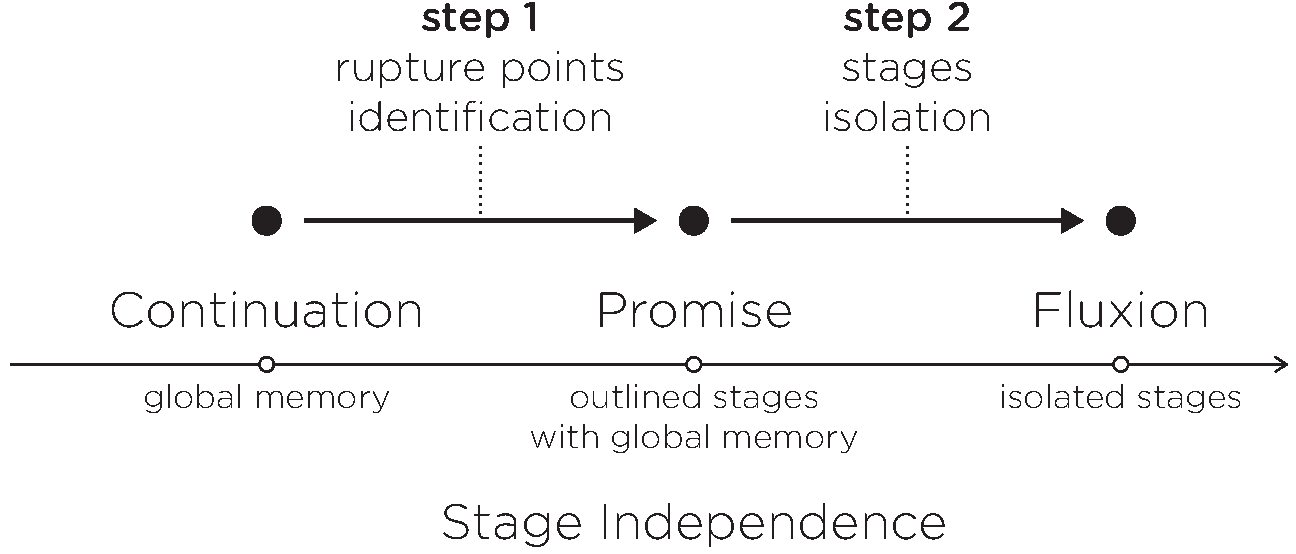
\includegraphics[width=0.7\textwidth]{../resources/roadmap.pdf}%
    \caption{Roadmap}%
    \label{fig:roadmap}%
  }%
\end{figure}

The first compiler focuses on the identification of simple chains of causality between continuations to transform these chains into Promises.
% the transformation from continuations to Promises.
% It focuses on the identification of the chains of causality in continuations.
However, promises are more expressive than the simple chaining of causal sequentiality.
% They force another control over the execution flow.
% According to the outcome of the operation, they call one function to continue the execution with the result, or another to handle errors.
% This conditional execution is indivisible from the Promise specification.
% Promises impose a convention on how to hand back the outcome of the deferred computation, while classic continuations leave this conditional execution to the developer.
Moreover, they impose a different convention than continuations on how to hand back the outcome and errors of the deferred computation.
This difference brings unnecessary complexity to the identification of chains.
To rule out this difference between continuations and Promises, before introducing the first compiler, section \ref{chapter5:due} introduces a simpler specification to Promise, called Due.

The second compiler detects all the chains of causality between continuations and encapsulate them in fluxions.
It isolates the fluxions when possible to allow the parallelism required for efficiency.
This second compilers is introduced in section \ref{chapter5:flx}.

\renewcommand{\glyph}{\iconfont{\XeTeXglyph287}}
\chapter{Implementations} \label{chapter5}
\minitoc
\eject
The transformation allowed by the equivalence from an event-driven program into a distributed network of fluxions is implemented incrementally into two compilers, as presented in figure \ref{fig:roadmap}.
Each compilers is divided into two steps, the identification of the rupture points separating the stages of the pipeline, and the isolation of these stages.
% This chapter presents the technical implementations of these two steps in the transformation from the event-driven execution model to the pipeline architecture
% , the transformation described in the previous chapter was implemented incrementally in two compilers.

\begin{figure}[h!]%
  \textfig{%
    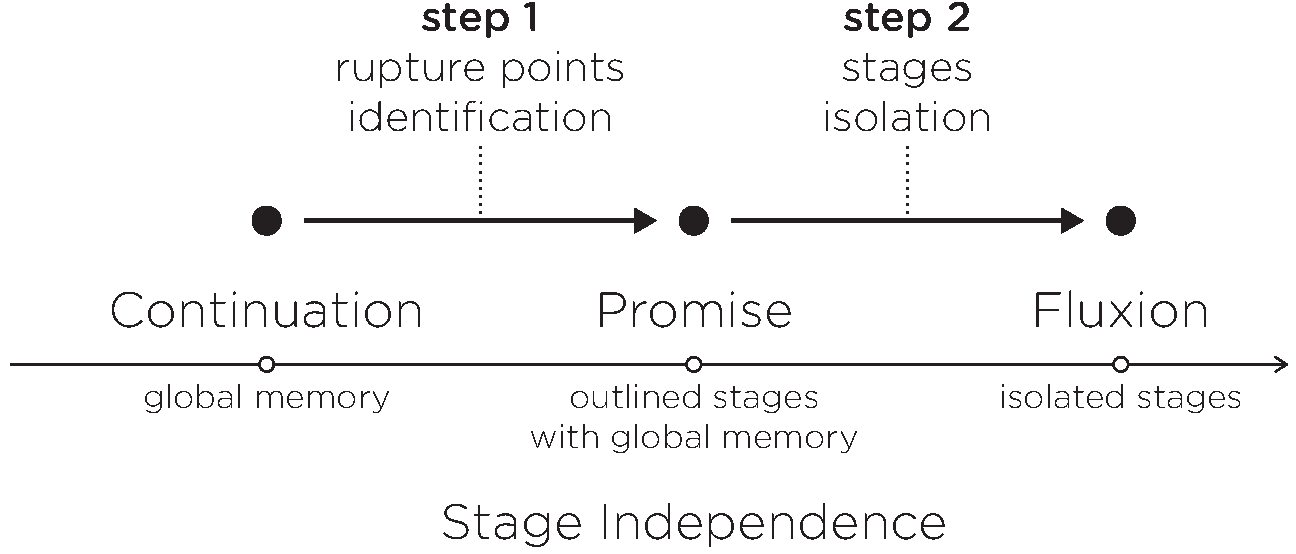
\includegraphics[width=0.7\textwidth]{../resources/roadmap.pdf}%
    \caption{Roadmap}%
    \label{fig:roadmap}%
  }%
\end{figure}

The first compiler focuses on the identification of simple chains of causality between continuations to transform these chains into Promises.
% the transformation from continuations to Promises.
% It focuses on the identification of the chains of causality in continuations.
However, promises are more expressive than the simple chaining of causal sequentiality.
% They force another control over the execution flow.
% According to the outcome of the operation, they call one function to continue the execution with the result, or another to handle errors.
% This conditional execution is indivisible from the Promise specification.
% Promises impose a convention on how to hand back the outcome of the deferred computation, while classic continuations leave this conditional execution to the developer.
Moreover, they impose a different convention than continuations on how to hand back the outcome and errors of the deferred computation.
This difference brings unnecessary complexity to the identification of chains.
To rule out this difference between continuations and Promises, before introducing the first compiler, section \ref{chapter5:due} introduces a simpler specification to Promise, called Due.

The second compiler detects all the chains of causality between continuations and encapsulate them in fluxions.
It isolates the fluxions when possible to allow the parallelism required for efficiency.
This second compilers is introduced in section \ref{chapter5:flx}.

\renewcommand{\glyph}{\iconfont{\XeTeXglyph287}}
\chapter{Implementations} \label{chapter5}
\minitoc
\eject
The transformation allowed by the equivalence from an event-driven program into a distributed network of fluxions is implemented incrementally into two compilers, as presented in figure \ref{fig:roadmap}.
Each compilers is divided into two steps, the identification of the rupture points separating the stages of the pipeline, and the isolation of these stages.
% This chapter presents the technical implementations of these two steps in the transformation from the event-driven execution model to the pipeline architecture
% , the transformation described in the previous chapter was implemented incrementally in two compilers.

\begin{figure}[h!]%
  \textfig{%
    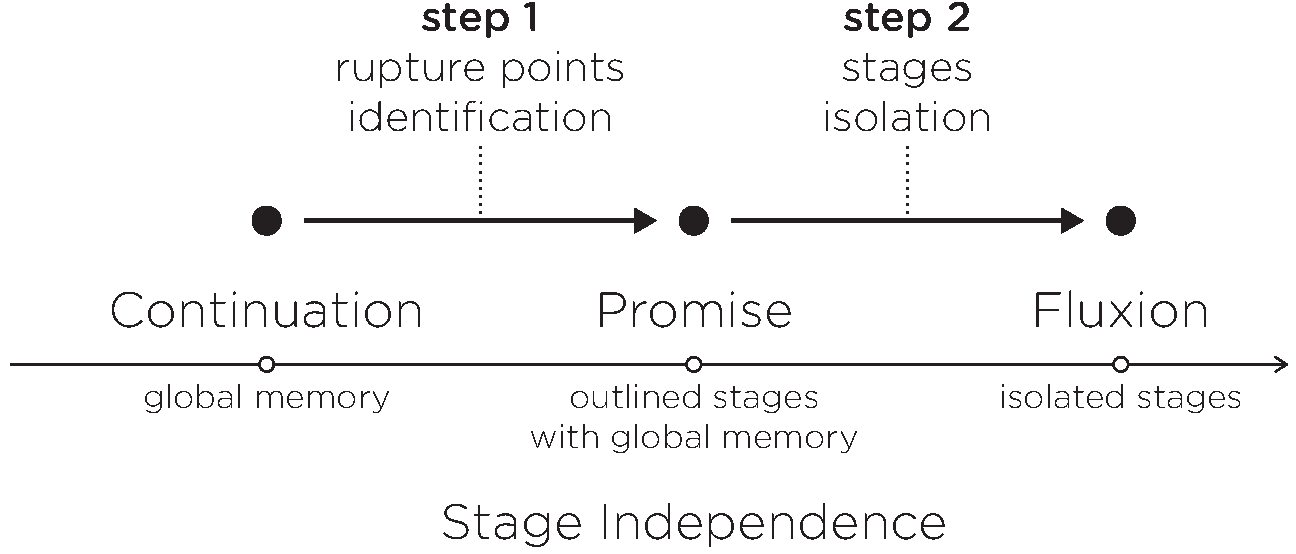
\includegraphics[width=0.7\textwidth]{../resources/roadmap.pdf}%
    \caption{Roadmap}%
    \label{fig:roadmap}%
  }%
\end{figure}

The first compiler focuses on the identification of simple chains of causality between continuations to transform these chains into Promises.
% the transformation from continuations to Promises.
% It focuses on the identification of the chains of causality in continuations.
However, promises are more expressive than the simple chaining of causal sequentiality.
% They force another control over the execution flow.
% According to the outcome of the operation, they call one function to continue the execution with the result, or another to handle errors.
% This conditional execution is indivisible from the Promise specification.
% Promises impose a convention on how to hand back the outcome of the deferred computation, while classic continuations leave this conditional execution to the developer.
Moreover, they impose a different convention than continuations on how to hand back the outcome and errors of the deferred computation.
This difference brings unnecessary complexity to the identification of chains.
To rule out this difference between continuations and Promises, before introducing the first compiler, section \ref{chapter5:due} introduces a simpler specification to Promise, called Due.

The second compiler detects all the chains of causality between continuations and encapsulate them in fluxions.
It isolates the fluxions when possible to allow the parallelism required for efficiency.
This second compilers is introduced in section \ref{chapter5:flx}.

\input{05-implementation/Due/main}
\input{05-implementation/Flx/main}
% \input{05-implementation/Evaluation}

\renewcommand{\glyph}{\iconfont{\XeTeXglyph287}}
\chapter{Implementations} \label{chapter5}
\minitoc
\eject
The transformation allowed by the equivalence from an event-driven program into a distributed network of fluxions is implemented incrementally into two compilers, as presented in figure \ref{fig:roadmap}.
Each compilers is divided into two steps, the identification of the rupture points separating the stages of the pipeline, and the isolation of these stages.
% This chapter presents the technical implementations of these two steps in the transformation from the event-driven execution model to the pipeline architecture
% , the transformation described in the previous chapter was implemented incrementally in two compilers.

\begin{figure}[h!]%
  \textfig{%
    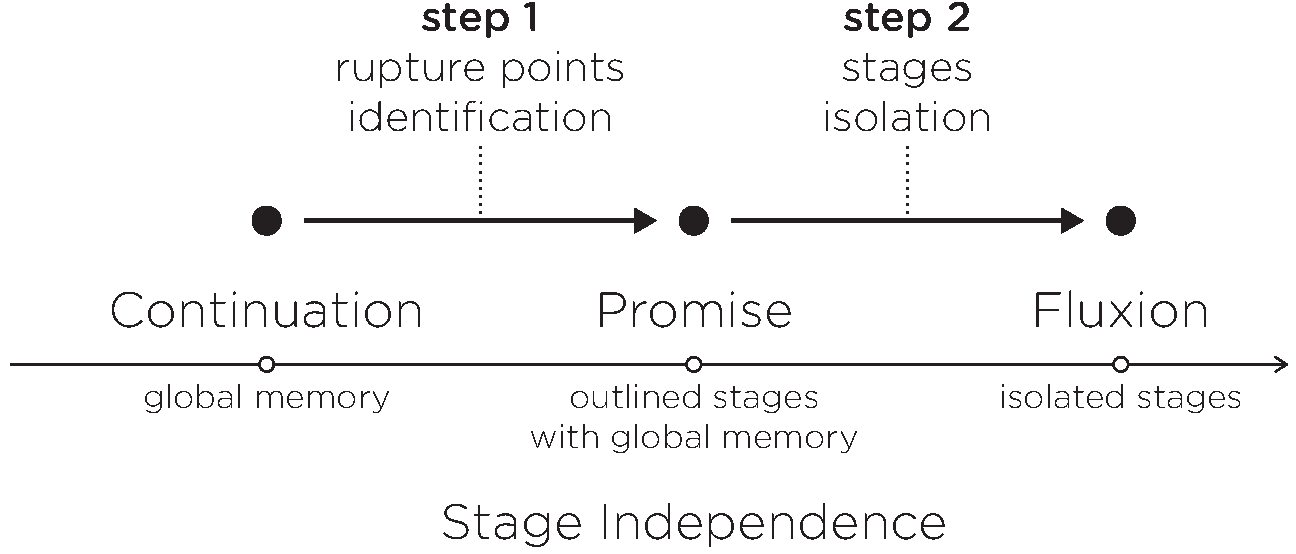
\includegraphics[width=0.7\textwidth]{../resources/roadmap.pdf}%
    \caption{Roadmap}%
    \label{fig:roadmap}%
  }%
\end{figure}

The first compiler focuses on the identification of simple chains of causality between continuations to transform these chains into Promises.
% the transformation from continuations to Promises.
% It focuses on the identification of the chains of causality in continuations.
However, promises are more expressive than the simple chaining of causal sequentiality.
% They force another control over the execution flow.
% According to the outcome of the operation, they call one function to continue the execution with the result, or another to handle errors.
% This conditional execution is indivisible from the Promise specification.
% Promises impose a convention on how to hand back the outcome of the deferred computation, while classic continuations leave this conditional execution to the developer.
Moreover, they impose a different convention than continuations on how to hand back the outcome and errors of the deferred computation.
This difference brings unnecessary complexity to the identification of chains.
To rule out this difference between continuations and Promises, before introducing the first compiler, section \ref{chapter5:due} introduces a simpler specification to Promise, called Due.

The second compiler detects all the chains of causality between continuations and encapsulate them in fluxions.
It isolates the fluxions when possible to allow the parallelism required for efficiency.
This second compilers is introduced in section \ref{chapter5:flx}.

\input{05-implementation/Due/main}
\input{05-implementation/Flx/main}
% \input{05-implementation/Evaluation}

% \subsection{Real test case} \label{chapter5:flx:evaluation}

The compiler is tested on a real application, gifsockets-server\ftnt{https://github.com/twolfson/gifsockets-server}.
This test proves the possibility for an application to be compiled into a network of independent parts.
It shows the current limitations of this isolation and the modifications needed on the application to circumvent them.

\begin{code}[js, caption={Simplified version of gifsockets-server},label={lst:gifsocket}]
var express = require('express'),
    app = express(),
    routes = require('gifsockets-middleware'), //@\label{lst:gifsocket:gif-mw}@
    getRawBody = require('raw-body');

function bodyParser(limit) { //@\label{lst:gifsocket:bodyParser}@
  return function saveBody(req, res, next) { //@\label{lst:gifsocket:saveBody}@
    getRawBody(req, { //@\label{lst:gifsocket:getRawBody}@
      expected: req.headers['content-length'],
      limit: limit
    }, function (err, buffer) { //@\label{lst:gifsocket:callback}@
      req.body = buffer;
      next(); //@\label{lst:gifsocket:next}@
    });
  };
}

app.post('/image/text', bodyParser(1 * 1024 * 1024), routes.writeTextToImages); //@\label{lst:gifsocket:app.post}@
app.listen(8000);
\end{code}

This application, simplified in listing \ref{lst:gifsocket}, is a real-time chat using gif-based communication channels.
It was selected from the evaluation set of the Due compiler because it is simple enough to illustrate this evaluation.
% \cite{Brodu2015}
%  from the \texttt{npm} registry because it depends on \texttt{express}, it is tested, working, and simple enough to illustrate this evaluation.
The server transforms the received text into a gif frame, and pushes it back to a never-ending gif to be displayed on the client.

On line \ref{lst:gifsocket:app.post}, the application registers two functions to process the requests received on the url \texttt{/image/text}.
The closure \texttt{saveBody}, line \ref{lst:gifsocket:saveBody}, returned by \texttt{bodyParser}, line \ref{lst:gifsocket:bodyParser}, and the method \texttt{routes.write\-Text\-To\-Images} from the external module \texttt{gifsockets-\-middleware}, line \ref{lst:gifsocket:gif-mw}.
The closure \texttt{saveBody} calls the asynchronous function \texttt{getRawBody} to get the request body.
Its callback handles the errors, and calls \texttt{next} to continue processing the request with the next function, \texttt{routes.write\-Text\-To\-Images}.

\subsubsection{Compilation} \label{chapter5:flx:evaluation:compilation}

% We compile this application with the compiler
The compilation result is in listing \ref{lst:flx-gifsocket}.
The function call \texttt{app.post}, line \ref{lst:gifsocket:app.post}, is a rupture point.
However, its callbacks, \texttt{bodyParser} and \texttt{routes.write\-Text\-To\-Images} are not declared \textit{in situ}.
They are evaluated as functions only at runtime.
As precised previously, the compiler discards these callbacks to avoid altering the semantic. % by moving or modifying their definition.
% For this reason, the compiler ignores this rupture point, to avoid interfering with the evaluation.

\begin{code}[flx, caption={Compilation result of gifsockets-server},label={lst:flx-gifsocket}]
flx main & express {req}
>> anonymous_1000 [req, next]
  var express = require('express'),
      app = express(),
      routes = require('gifsockets-middleware'), //@\label{lst:flx-gifsocket:gif-mw}@
      getRawBody = require('raw-body');

  function bodyParser(limit) { //@\label{lst:flx-gifsocket:bodyParser}@
    return function saveBody(req, res, next) { //@\label{lst:flx-gifsocket:saveBody}@
      getRawBody(req, { //@\label{lst:flx-gifsocket:getRawBody}@
        expected: req.headers['content-length'], //@\label{lst:flx-gifsocket:req.headers}@
        limit: limit
      }, >> anonymous_1000 [req, next]);
    };
  }

  app.post('/image/text', bodyParser(1 * 1024 * 1024), routes.writeTextToImages); //@\label{lst:flx-gifsocket:app.post}@
  app.listen(8000);

flx anonymous_1000
-> null
  function (err, buffer) { //@\label{lst:flx-gifsocket:callback}@
    req.body = buffer; //@\label{lst:flx-gifsocket:buffer}@
    next(); //@\label{lst:flx-gifsocket:next}@
  }
\end{code}

The compiler detects a rupture point : the function \texttt{get\-Raw\-Body} and its anonymous callback, line \ref{lst:gifsocket:callback}.
It encapsulates this callback in a fluxion named \texttt{anony\-mous\_\-1000}.
The callback is replaced with a stream placeholder to send the message stream to this downstream fluxion.
The variables \texttt{req} and \texttt{next} are appended to this message stream, to propagate their value from the \texttt{main} fluxion to the \texttt{anony\-mous\_\-1000} fluxion.

When \texttt{anony\-mous\_\-1000} is not isolated from the \texttt{main} fluxion, as if they belong to the same group, the compilation result works as expected.
The variables used in the fluxion, \texttt{req} and \texttt{next}, are still shared between the two fluxions.
In this situation fluxions are quite similar to Dues regarding memory shareing.
Our goal is to isolate the two fluxions, to be able to safely parallelize their executions.

\subsubsection{Isolation} \label{chapter5:flx:evaluation:isolation}

In listing \ref{lst:flx-gifsocket}, the fluxion \texttt{anony\-mous\_\-1000} modifies the object \texttt{req}, line \ref{lst:flx-gifsocket:buffer}, to store the text of the received request, and it calls \texttt{next} to continue the execution, line \ref{lst:flx-gifsocket:next}.
\texttt{req} is an alias to a memory location used in multiple palces in code.
Therefore, these operations produce side-effects that should propagate in the whole application, but the isolation prevents this propagation.
Isolating the fluxion \texttt{anony\-mous\_\-1000} produces runtime exceptions.
The next paragraph details how this situation is handled to allow the application to be parallelized.

\paragraph{Variable \texttt{req}}

The variable \texttt{req} is read in fluxion \texttt{main}, lines \ref{lst:flx-gifsocket:getRawBody} and \ref{lst:flx-gifsocket:req.headers}.
Then its property \texttt{body} is associated to \texttt{buffer} in fluxion \texttt{anony\-mous\_\-1000}, line \ref{lst:flx-gifsocket:buffer}.
The compiler is unable to identify the aliases of this variable. % further usages.
However, the side effect resulting from this association impacts a variable in the scope of the next callback, \texttt{routes.write\-Text\-To\-Images}.
In this test case, the application is modified manually to explicitly propagate this side-effect to the next callback through the function \texttt{next}.
The modifications of this function are explained further in the next paragraph.

\paragraph{Closure \texttt{next}}

The function \texttt{next} is a closure provided by the \texttt{express} \texttt{Router} to continue the execution with the next function to handle the client request.
Because it indirectly relies on the variable \texttt{req}, it is impossible to isolate its execution with the \texttt{anony\-mous\_\-1000} fluxion.
Instead, we modify \texttt{express}, so as to be compatible with the fluxional execution model.
We explain the modifications below.

\begin{code}[flx, caption={Simplified modification on the compiled result},label={lst:mflx-gifsocket}]
flx anonymous_1000
-> express_dispatcher
  function (err, buffer) { //@\label{lst:mflx-gifsocket:callback}@
    req.body = buffer; //@\label{lst:mflx-gifsocket:buffer}@
    next_placeholder(req, -> express_dispatcher); //@\label{lst:mflx-gifsocket:next-placeholder}@
  }

flx express_dispatcher & express {req} //@\label{lst:mflx-gifsocket:express-dispatcher}@
-> null
  function (modified_req) {
    merge(req, modified_req);
    next(); //@\label{lst:mflx-gifsocket:next}@
  }
\end{code}

In listing \ref{lst:gifsocket}, the function \texttt{next} is a continuation allowing the anonymous callback, line \ref{lst:gifsocket:callback}, to call the next function to handle the request.
To isolate the anonymous callback into \texttt{anonymous\_\-1000}, \texttt{next} is replaced by a rupture point.
This replacement is illustrated in listing \ref{lst:mflx-gifsocket}.
The \texttt{express} \texttt{Router} registers a fluxion named \texttt{express\_\-dispatcher}, line \ref{lst:mflx-gifsocket:express-dispatcher}, to continue the execution after the fluxion \texttt{anony\-mous\_\-1000}.
This fluxion is in the same group \texttt{express} as the \texttt{main} fluxion, hence it has access to the original variable \texttt{req}, and to the original function \texttt{next}.
The call to the original \texttt{next} function is replaced by a placeholder to push the stream to the fluxion \texttt{express\_\-dispatcher}, line \ref{lst:mflx-gifsocket:next-placeholder}.
The fluxion \texttt{express\_\-dispatcher} receives the stream from the upstream fluxion \texttt{anony\-mous\_\-1000}, merges back the modification in the variable \texttt{req} to propagate the side effects, and finally calls the original function \texttt{next} to continue the execution, line \ref{lst:mflx-gifsocket:next}.

After the modifications detailed above, the server works as expected.
The isolated fluxion correctly receives, and returns its serialized messages.
The client successfully receives a gif frame containing the text.



\subsection{Limitations}

The static analysis used for this compiler presents some limitations.
It is unable to analyze code with dynamic behaviors.
Higher-order programming leads to more productivity partly beacuse it rely on such dynamic behavior to extend expressivity.
Precisely, it allows more levels of indirections.

\subsubsection{Levels of Indirections}

The indirection is an abstraction between the value, and its manipulation.
In listing \ref{lst:indirection}, the variables \texttt{a} and \texttt{b} point both to the same memory object.
The function \texttt{fn} introduces a level of indirection between the real object \texttt{a} and its manipulation handle, \texttt{b};
% Actually, the variable \texttt{a} already introduces a level of indirection between the real object and the handle \texttt{a}.

\begin{code}[js,
  caption={One level of Indirection},
  label={lst:indirection}]
var a = {
      // an object;
    };

fn(b) {
  // modify b;
}

fn(a);
\end{code}

\subsubsection{Uncertainties}

The indirection is trivial to resolve in listing \ref{lst:indirection}.
It only needs to have access to the definition of \texttt{a} and of \texttt{fn}.
%A very simple static analysis could resolve it.
However, in listing \ref{lst:indirections}, the array \texttt{handlers} introduces a new level of indirection.
The static analysis now needs to have access to the definition of \texttt{i} and of the \texttt{handlers}.
If this definition is provided by an external input, it is not available statically, hence, it adds an uncertainty during the analysis. 

\begin{code}[js,
  caption={Two levels of indirection},
  label={lst:indirections}]
var a = {
      // an object;
    },
    handlers = [
      // definition of fn handlers;
    ],
    i = ?;

handlers[i](a);
handlers[i+1](a);
\end{code}

These examples are extremely simplified.
A real application contains enough indirections for the static analysis to be overwhelmed by uncertainties, and to be unable to resolve the variables.
If a variable is left unresolved, it is impossible to assure its scope and its aliases.
Therefore, the compiler is unable to isolate it into a fluxion, or to distribute its modification by messages.

Moreover, it leads the compiler to ignore the rupture points not defined \textit{in situ}, because their modifications could impact the semantic.
The reason for this precaution, is that the compiler is unable to assure where the function is used, and the scope of its variables.
Therefore, it is unable to assure that the modification will conserve the semantic.

\subsubsection{Dynamic Resolution}

In a web application, this variable \texttt{i} might be part of the user request, which is available only at runtime.
It eventually introduces an uncertainty.

This dynamic resolution of variables is precisely what increase expressiveness.
Trying to resolve them statically is equivalent to restrict expressiveness.
No static analysis can overstep these limitations.
Only a dynamic analysis could analysis the resolved indirections during run time to overstep these limitations correctly.




\renewcommand{\glyph}{\iconfont{\XeTeXglyph287}}
\chapter{Implementations} \label{chapter5}
\minitoc
\eject
The transformation allowed by the equivalence from an event-driven program into a distributed network of fluxions is implemented incrementally into two compilers, as presented in figure \ref{fig:roadmap}.
Each compilers is divided into two steps, the identification of the rupture points separating the stages of the pipeline, and the isolation of these stages.
% This chapter presents the technical implementations of these two steps in the transformation from the event-driven execution model to the pipeline architecture
% , the transformation described in the previous chapter was implemented incrementally in two compilers.

\begin{figure}[h!]%
  \textfig{%
    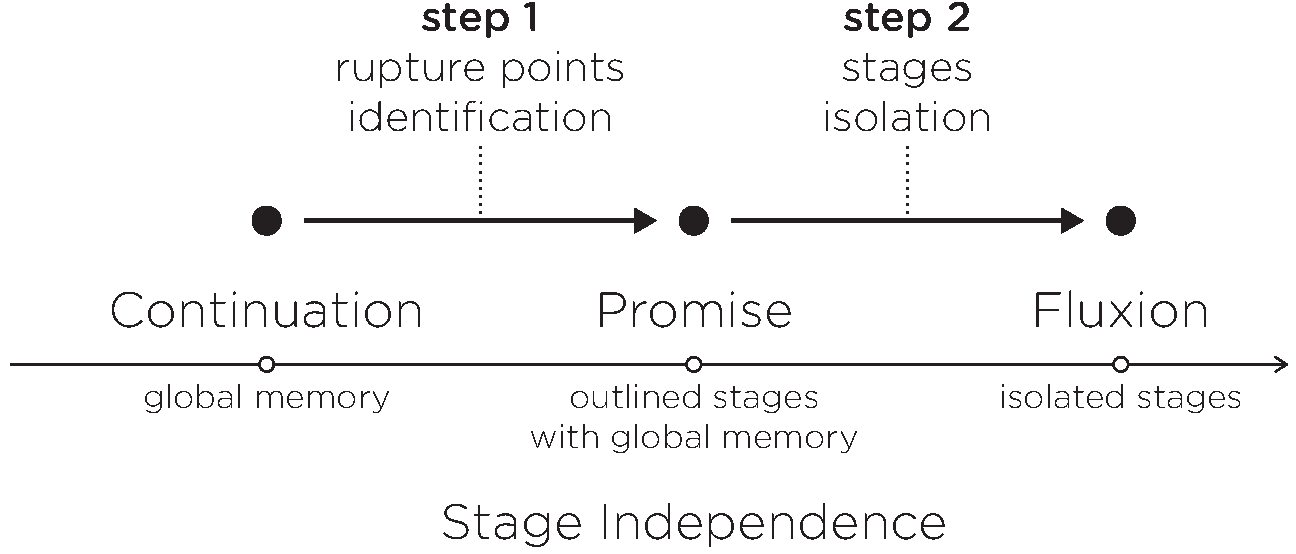
\includegraphics[width=0.7\textwidth]{../resources/roadmap.pdf}%
    \caption{Roadmap}%
    \label{fig:roadmap}%
  }%
\end{figure}

The first compiler focuses on the identification of simple chains of causality between continuations to transform these chains into Promises.
% the transformation from continuations to Promises.
% It focuses on the identification of the chains of causality in continuations.
However, promises are more expressive than the simple chaining of causal sequentiality.
% They force another control over the execution flow.
% According to the outcome of the operation, they call one function to continue the execution with the result, or another to handle errors.
% This conditional execution is indivisible from the Promise specification.
% Promises impose a convention on how to hand back the outcome of the deferred computation, while classic continuations leave this conditional execution to the developer.
Moreover, they impose a different convention than continuations on how to hand back the outcome and errors of the deferred computation.
This difference brings unnecessary complexity to the identification of chains.
To rule out this difference between continuations and Promises, before introducing the first compiler, section \ref{chapter5:due} introduces a simpler specification to Promise, called Due.

The second compiler detects all the chains of causality between continuations and encapsulate them in fluxions.
It isolates the fluxions when possible to allow the parallelism required for efficiency.
This second compilers is introduced in section \ref{chapter5:flx}.

\renewcommand{\glyph}{\iconfont{\XeTeXglyph287}}
\chapter{Implementations} \label{chapter5}
\minitoc
\eject
The transformation allowed by the equivalence from an event-driven program into a distributed network of fluxions is implemented incrementally into two compilers, as presented in figure \ref{fig:roadmap}.
Each compilers is divided into two steps, the identification of the rupture points separating the stages of the pipeline, and the isolation of these stages.
% This chapter presents the technical implementations of these two steps in the transformation from the event-driven execution model to the pipeline architecture
% , the transformation described in the previous chapter was implemented incrementally in two compilers.

\begin{figure}[h!]%
  \textfig{%
    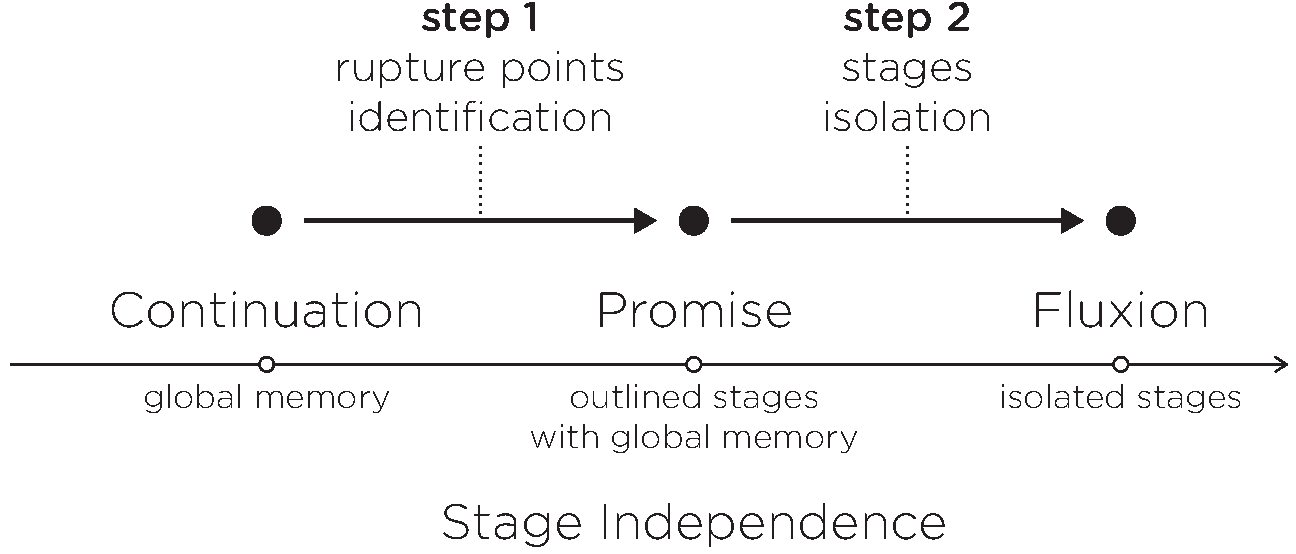
\includegraphics[width=0.7\textwidth]{../resources/roadmap.pdf}%
    \caption{Roadmap}%
    \label{fig:roadmap}%
  }%
\end{figure}

The first compiler focuses on the identification of simple chains of causality between continuations to transform these chains into Promises.
% the transformation from continuations to Promises.
% It focuses on the identification of the chains of causality in continuations.
However, promises are more expressive than the simple chaining of causal sequentiality.
% They force another control over the execution flow.
% According to the outcome of the operation, they call one function to continue the execution with the result, or another to handle errors.
% This conditional execution is indivisible from the Promise specification.
% Promises impose a convention on how to hand back the outcome of the deferred computation, while classic continuations leave this conditional execution to the developer.
Moreover, they impose a different convention than continuations on how to hand back the outcome and errors of the deferred computation.
This difference brings unnecessary complexity to the identification of chains.
To rule out this difference between continuations and Promises, before introducing the first compiler, section \ref{chapter5:due} introduces a simpler specification to Promise, called Due.

The second compiler detects all the chains of causality between continuations and encapsulate them in fluxions.
It isolates the fluxions when possible to allow the parallelism required for efficiency.
This second compilers is introduced in section \ref{chapter5:flx}.

\input{05-implementation/Due/main}
\input{05-implementation/Flx/main}
% \input{05-implementation/Evaluation}

\renewcommand{\glyph}{\iconfont{\XeTeXglyph287}}
\chapter{Implementations} \label{chapter5}
\minitoc
\eject
The transformation allowed by the equivalence from an event-driven program into a distributed network of fluxions is implemented incrementally into two compilers, as presented in figure \ref{fig:roadmap}.
Each compilers is divided into two steps, the identification of the rupture points separating the stages of the pipeline, and the isolation of these stages.
% This chapter presents the technical implementations of these two steps in the transformation from the event-driven execution model to the pipeline architecture
% , the transformation described in the previous chapter was implemented incrementally in two compilers.

\begin{figure}[h!]%
  \textfig{%
    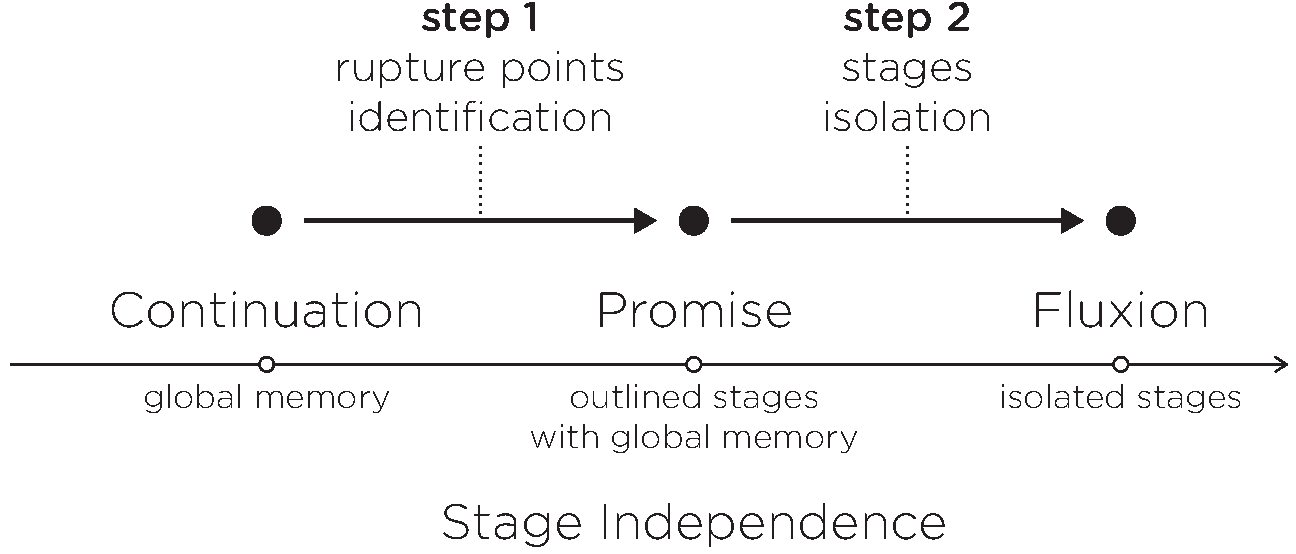
\includegraphics[width=0.7\textwidth]{../resources/roadmap.pdf}%
    \caption{Roadmap}%
    \label{fig:roadmap}%
  }%
\end{figure}

The first compiler focuses on the identification of simple chains of causality between continuations to transform these chains into Promises.
% the transformation from continuations to Promises.
% It focuses on the identification of the chains of causality in continuations.
However, promises are more expressive than the simple chaining of causal sequentiality.
% They force another control over the execution flow.
% According to the outcome of the operation, they call one function to continue the execution with the result, or another to handle errors.
% This conditional execution is indivisible from the Promise specification.
% Promises impose a convention on how to hand back the outcome of the deferred computation, while classic continuations leave this conditional execution to the developer.
Moreover, they impose a different convention than continuations on how to hand back the outcome and errors of the deferred computation.
This difference brings unnecessary complexity to the identification of chains.
To rule out this difference between continuations and Promises, before introducing the first compiler, section \ref{chapter5:due} introduces a simpler specification to Promise, called Due.

The second compiler detects all the chains of causality between continuations and encapsulate them in fluxions.
It isolates the fluxions when possible to allow the parallelism required for efficiency.
This second compilers is introduced in section \ref{chapter5:flx}.

\input{05-implementation/Due/main}
\input{05-implementation/Flx/main}
% \input{05-implementation/Evaluation}

% \subsection{Real test case} \label{chapter5:flx:evaluation}

The compiler is tested on a real application, gifsockets-server\ftnt{https://github.com/twolfson/gifsockets-server}.
This test proves the possibility for an application to be compiled into a network of independent parts.
It shows the current limitations of this isolation and the modifications needed on the application to circumvent them.

\begin{code}[js, caption={Simplified version of gifsockets-server},label={lst:gifsocket}]
var express = require('express'),
    app = express(),
    routes = require('gifsockets-middleware'), //@\label{lst:gifsocket:gif-mw}@
    getRawBody = require('raw-body');

function bodyParser(limit) { //@\label{lst:gifsocket:bodyParser}@
  return function saveBody(req, res, next) { //@\label{lst:gifsocket:saveBody}@
    getRawBody(req, { //@\label{lst:gifsocket:getRawBody}@
      expected: req.headers['content-length'],
      limit: limit
    }, function (err, buffer) { //@\label{lst:gifsocket:callback}@
      req.body = buffer;
      next(); //@\label{lst:gifsocket:next}@
    });
  };
}

app.post('/image/text', bodyParser(1 * 1024 * 1024), routes.writeTextToImages); //@\label{lst:gifsocket:app.post}@
app.listen(8000);
\end{code}

This application, simplified in listing \ref{lst:gifsocket}, is a real-time chat using gif-based communication channels.
It was selected from the evaluation set of the Due compiler because it is simple enough to illustrate this evaluation.
% \cite{Brodu2015}
%  from the \texttt{npm} registry because it depends on \texttt{express}, it is tested, working, and simple enough to illustrate this evaluation.
The server transforms the received text into a gif frame, and pushes it back to a never-ending gif to be displayed on the client.

On line \ref{lst:gifsocket:app.post}, the application registers two functions to process the requests received on the url \texttt{/image/text}.
The closure \texttt{saveBody}, line \ref{lst:gifsocket:saveBody}, returned by \texttt{bodyParser}, line \ref{lst:gifsocket:bodyParser}, and the method \texttt{routes.write\-Text\-To\-Images} from the external module \texttt{gifsockets-\-middleware}, line \ref{lst:gifsocket:gif-mw}.
The closure \texttt{saveBody} calls the asynchronous function \texttt{getRawBody} to get the request body.
Its callback handles the errors, and calls \texttt{next} to continue processing the request with the next function, \texttt{routes.write\-Text\-To\-Images}.

\subsubsection{Compilation} \label{chapter5:flx:evaluation:compilation}

% We compile this application with the compiler
The compilation result is in listing \ref{lst:flx-gifsocket}.
The function call \texttt{app.post}, line \ref{lst:gifsocket:app.post}, is a rupture point.
However, its callbacks, \texttt{bodyParser} and \texttt{routes.write\-Text\-To\-Images} are not declared \textit{in situ}.
They are evaluated as functions only at runtime.
As precised previously, the compiler discards these callbacks to avoid altering the semantic. % by moving or modifying their definition.
% For this reason, the compiler ignores this rupture point, to avoid interfering with the evaluation.

\begin{code}[flx, caption={Compilation result of gifsockets-server},label={lst:flx-gifsocket}]
flx main & express {req}
>> anonymous_1000 [req, next]
  var express = require('express'),
      app = express(),
      routes = require('gifsockets-middleware'), //@\label{lst:flx-gifsocket:gif-mw}@
      getRawBody = require('raw-body');

  function bodyParser(limit) { //@\label{lst:flx-gifsocket:bodyParser}@
    return function saveBody(req, res, next) { //@\label{lst:flx-gifsocket:saveBody}@
      getRawBody(req, { //@\label{lst:flx-gifsocket:getRawBody}@
        expected: req.headers['content-length'], //@\label{lst:flx-gifsocket:req.headers}@
        limit: limit
      }, >> anonymous_1000 [req, next]);
    };
  }

  app.post('/image/text', bodyParser(1 * 1024 * 1024), routes.writeTextToImages); //@\label{lst:flx-gifsocket:app.post}@
  app.listen(8000);

flx anonymous_1000
-> null
  function (err, buffer) { //@\label{lst:flx-gifsocket:callback}@
    req.body = buffer; //@\label{lst:flx-gifsocket:buffer}@
    next(); //@\label{lst:flx-gifsocket:next}@
  }
\end{code}

The compiler detects a rupture point : the function \texttt{get\-Raw\-Body} and its anonymous callback, line \ref{lst:gifsocket:callback}.
It encapsulates this callback in a fluxion named \texttt{anony\-mous\_\-1000}.
The callback is replaced with a stream placeholder to send the message stream to this downstream fluxion.
The variables \texttt{req} and \texttt{next} are appended to this message stream, to propagate their value from the \texttt{main} fluxion to the \texttt{anony\-mous\_\-1000} fluxion.

When \texttt{anony\-mous\_\-1000} is not isolated from the \texttt{main} fluxion, as if they belong to the same group, the compilation result works as expected.
The variables used in the fluxion, \texttt{req} and \texttt{next}, are still shared between the two fluxions.
In this situation fluxions are quite similar to Dues regarding memory shareing.
Our goal is to isolate the two fluxions, to be able to safely parallelize their executions.

\subsubsection{Isolation} \label{chapter5:flx:evaluation:isolation}

In listing \ref{lst:flx-gifsocket}, the fluxion \texttt{anony\-mous\_\-1000} modifies the object \texttt{req}, line \ref{lst:flx-gifsocket:buffer}, to store the text of the received request, and it calls \texttt{next} to continue the execution, line \ref{lst:flx-gifsocket:next}.
\texttt{req} is an alias to a memory location used in multiple palces in code.
Therefore, these operations produce side-effects that should propagate in the whole application, but the isolation prevents this propagation.
Isolating the fluxion \texttt{anony\-mous\_\-1000} produces runtime exceptions.
The next paragraph details how this situation is handled to allow the application to be parallelized.

\paragraph{Variable \texttt{req}}

The variable \texttt{req} is read in fluxion \texttt{main}, lines \ref{lst:flx-gifsocket:getRawBody} and \ref{lst:flx-gifsocket:req.headers}.
Then its property \texttt{body} is associated to \texttt{buffer} in fluxion \texttt{anony\-mous\_\-1000}, line \ref{lst:flx-gifsocket:buffer}.
The compiler is unable to identify the aliases of this variable. % further usages.
However, the side effect resulting from this association impacts a variable in the scope of the next callback, \texttt{routes.write\-Text\-To\-Images}.
In this test case, the application is modified manually to explicitly propagate this side-effect to the next callback through the function \texttt{next}.
The modifications of this function are explained further in the next paragraph.

\paragraph{Closure \texttt{next}}

The function \texttt{next} is a closure provided by the \texttt{express} \texttt{Router} to continue the execution with the next function to handle the client request.
Because it indirectly relies on the variable \texttt{req}, it is impossible to isolate its execution with the \texttt{anony\-mous\_\-1000} fluxion.
Instead, we modify \texttt{express}, so as to be compatible with the fluxional execution model.
We explain the modifications below.

\begin{code}[flx, caption={Simplified modification on the compiled result},label={lst:mflx-gifsocket}]
flx anonymous_1000
-> express_dispatcher
  function (err, buffer) { //@\label{lst:mflx-gifsocket:callback}@
    req.body = buffer; //@\label{lst:mflx-gifsocket:buffer}@
    next_placeholder(req, -> express_dispatcher); //@\label{lst:mflx-gifsocket:next-placeholder}@
  }

flx express_dispatcher & express {req} //@\label{lst:mflx-gifsocket:express-dispatcher}@
-> null
  function (modified_req) {
    merge(req, modified_req);
    next(); //@\label{lst:mflx-gifsocket:next}@
  }
\end{code}

In listing \ref{lst:gifsocket}, the function \texttt{next} is a continuation allowing the anonymous callback, line \ref{lst:gifsocket:callback}, to call the next function to handle the request.
To isolate the anonymous callback into \texttt{anonymous\_\-1000}, \texttt{next} is replaced by a rupture point.
This replacement is illustrated in listing \ref{lst:mflx-gifsocket}.
The \texttt{express} \texttt{Router} registers a fluxion named \texttt{express\_\-dispatcher}, line \ref{lst:mflx-gifsocket:express-dispatcher}, to continue the execution after the fluxion \texttt{anony\-mous\_\-1000}.
This fluxion is in the same group \texttt{express} as the \texttt{main} fluxion, hence it has access to the original variable \texttt{req}, and to the original function \texttt{next}.
The call to the original \texttt{next} function is replaced by a placeholder to push the stream to the fluxion \texttt{express\_\-dispatcher}, line \ref{lst:mflx-gifsocket:next-placeholder}.
The fluxion \texttt{express\_\-dispatcher} receives the stream from the upstream fluxion \texttt{anony\-mous\_\-1000}, merges back the modification in the variable \texttt{req} to propagate the side effects, and finally calls the original function \texttt{next} to continue the execution, line \ref{lst:mflx-gifsocket:next}.

After the modifications detailed above, the server works as expected.
The isolated fluxion correctly receives, and returns its serialized messages.
The client successfully receives a gif frame containing the text.



\subsection{Limitations}

The static analysis used for this compiler presents some limitations.
It is unable to analyze code with dynamic behaviors.
Higher-order programming leads to more productivity partly beacuse it rely on such dynamic behavior to extend expressivity.
Precisely, it allows more levels of indirections.

\subsubsection{Levels of Indirections}

The indirection is an abstraction between the value, and its manipulation.
In listing \ref{lst:indirection}, the variables \texttt{a} and \texttt{b} point both to the same memory object.
The function \texttt{fn} introduces a level of indirection between the real object \texttt{a} and its manipulation handle, \texttt{b};
% Actually, the variable \texttt{a} already introduces a level of indirection between the real object and the handle \texttt{a}.

\begin{code}[js,
  caption={One level of Indirection},
  label={lst:indirection}]
var a = {
      // an object;
    };

fn(b) {
  // modify b;
}

fn(a);
\end{code}

\subsubsection{Uncertainties}

The indirection is trivial to resolve in listing \ref{lst:indirection}.
It only needs to have access to the definition of \texttt{a} and of \texttt{fn}.
%A very simple static analysis could resolve it.
However, in listing \ref{lst:indirections}, the array \texttt{handlers} introduces a new level of indirection.
The static analysis now needs to have access to the definition of \texttt{i} and of the \texttt{handlers}.
If this definition is provided by an external input, it is not available statically, hence, it adds an uncertainty during the analysis. 

\begin{code}[js,
  caption={Two levels of indirection},
  label={lst:indirections}]
var a = {
      // an object;
    },
    handlers = [
      // definition of fn handlers;
    ],
    i = ?;

handlers[i](a);
handlers[i+1](a);
\end{code}

These examples are extremely simplified.
A real application contains enough indirections for the static analysis to be overwhelmed by uncertainties, and to be unable to resolve the variables.
If a variable is left unresolved, it is impossible to assure its scope and its aliases.
Therefore, the compiler is unable to isolate it into a fluxion, or to distribute its modification by messages.

Moreover, it leads the compiler to ignore the rupture points not defined \textit{in situ}, because their modifications could impact the semantic.
The reason for this precaution, is that the compiler is unable to assure where the function is used, and the scope of its variables.
Therefore, it is unable to assure that the modification will conserve the semantic.

\subsubsection{Dynamic Resolution}

In a web application, this variable \texttt{i} might be part of the user request, which is available only at runtime.
It eventually introduces an uncertainty.

This dynamic resolution of variables is precisely what increase expressiveness.
Trying to resolve them statically is equivalent to restrict expressiveness.
No static analysis can overstep these limitations.
Only a dynamic analysis could analysis the resolved indirections during run time to overstep these limitations correctly.




% \subsection{Real test case} \label{chapter5:flx:evaluation}

The compiler is tested on a real application, gifsockets-server\ftnt{https://github.com/twolfson/gifsockets-server}.
This test proves the possibility for an application to be compiled into a network of independent parts.
It shows the current limitations of this isolation and the modifications needed on the application to circumvent them.

\begin{code}[js, caption={Simplified version of gifsockets-server},label={lst:gifsocket}]
var express = require('express'),
    app = express(),
    routes = require('gifsockets-middleware'), //@\label{lst:gifsocket:gif-mw}@
    getRawBody = require('raw-body');

function bodyParser(limit) { //@\label{lst:gifsocket:bodyParser}@
  return function saveBody(req, res, next) { //@\label{lst:gifsocket:saveBody}@
    getRawBody(req, { //@\label{lst:gifsocket:getRawBody}@
      expected: req.headers['content-length'],
      limit: limit
    }, function (err, buffer) { //@\label{lst:gifsocket:callback}@
      req.body = buffer;
      next(); //@\label{lst:gifsocket:next}@
    });
  };
}

app.post('/image/text', bodyParser(1 * 1024 * 1024), routes.writeTextToImages); //@\label{lst:gifsocket:app.post}@
app.listen(8000);
\end{code}

This application, simplified in listing \ref{lst:gifsocket}, is a real-time chat using gif-based communication channels.
It was selected from the evaluation set of the Due compiler because it is simple enough to illustrate this evaluation.
% \cite{Brodu2015}
%  from the \texttt{npm} registry because it depends on \texttt{express}, it is tested, working, and simple enough to illustrate this evaluation.
The server transforms the received text into a gif frame, and pushes it back to a never-ending gif to be displayed on the client.

On line \ref{lst:gifsocket:app.post}, the application registers two functions to process the requests received on the url \texttt{/image/text}.
The closure \texttt{saveBody}, line \ref{lst:gifsocket:saveBody}, returned by \texttt{bodyParser}, line \ref{lst:gifsocket:bodyParser}, and the method \texttt{routes.write\-Text\-To\-Images} from the external module \texttt{gifsockets-\-middleware}, line \ref{lst:gifsocket:gif-mw}.
The closure \texttt{saveBody} calls the asynchronous function \texttt{getRawBody} to get the request body.
Its callback handles the errors, and calls \texttt{next} to continue processing the request with the next function, \texttt{routes.write\-Text\-To\-Images}.

\subsubsection{Compilation} \label{chapter5:flx:evaluation:compilation}

% We compile this application with the compiler
The compilation result is in listing \ref{lst:flx-gifsocket}.
The function call \texttt{app.post}, line \ref{lst:gifsocket:app.post}, is a rupture point.
However, its callbacks, \texttt{bodyParser} and \texttt{routes.write\-Text\-To\-Images} are not declared \textit{in situ}.
They are evaluated as functions only at runtime.
As precised previously, the compiler discards these callbacks to avoid altering the semantic. % by moving or modifying their definition.
% For this reason, the compiler ignores this rupture point, to avoid interfering with the evaluation.

\begin{code}[flx, caption={Compilation result of gifsockets-server},label={lst:flx-gifsocket}]
flx main & express {req}
>> anonymous_1000 [req, next]
  var express = require('express'),
      app = express(),
      routes = require('gifsockets-middleware'), //@\label{lst:flx-gifsocket:gif-mw}@
      getRawBody = require('raw-body');

  function bodyParser(limit) { //@\label{lst:flx-gifsocket:bodyParser}@
    return function saveBody(req, res, next) { //@\label{lst:flx-gifsocket:saveBody}@
      getRawBody(req, { //@\label{lst:flx-gifsocket:getRawBody}@
        expected: req.headers['content-length'], //@\label{lst:flx-gifsocket:req.headers}@
        limit: limit
      }, >> anonymous_1000 [req, next]);
    };
  }

  app.post('/image/text', bodyParser(1 * 1024 * 1024), routes.writeTextToImages); //@\label{lst:flx-gifsocket:app.post}@
  app.listen(8000);

flx anonymous_1000
-> null
  function (err, buffer) { //@\label{lst:flx-gifsocket:callback}@
    req.body = buffer; //@\label{lst:flx-gifsocket:buffer}@
    next(); //@\label{lst:flx-gifsocket:next}@
  }
\end{code}

The compiler detects a rupture point : the function \texttt{get\-Raw\-Body} and its anonymous callback, line \ref{lst:gifsocket:callback}.
It encapsulates this callback in a fluxion named \texttt{anony\-mous\_\-1000}.
The callback is replaced with a stream placeholder to send the message stream to this downstream fluxion.
The variables \texttt{req} and \texttt{next} are appended to this message stream, to propagate their value from the \texttt{main} fluxion to the \texttt{anony\-mous\_\-1000} fluxion.

When \texttt{anony\-mous\_\-1000} is not isolated from the \texttt{main} fluxion, as if they belong to the same group, the compilation result works as expected.
The variables used in the fluxion, \texttt{req} and \texttt{next}, are still shared between the two fluxions.
In this situation fluxions are quite similar to Dues regarding memory shareing.
Our goal is to isolate the two fluxions, to be able to safely parallelize their executions.

\subsubsection{Isolation} \label{chapter5:flx:evaluation:isolation}

In listing \ref{lst:flx-gifsocket}, the fluxion \texttt{anony\-mous\_\-1000} modifies the object \texttt{req}, line \ref{lst:flx-gifsocket:buffer}, to store the text of the received request, and it calls \texttt{next} to continue the execution, line \ref{lst:flx-gifsocket:next}.
\texttt{req} is an alias to a memory location used in multiple palces in code.
Therefore, these operations produce side-effects that should propagate in the whole application, but the isolation prevents this propagation.
Isolating the fluxion \texttt{anony\-mous\_\-1000} produces runtime exceptions.
The next paragraph details how this situation is handled to allow the application to be parallelized.

\paragraph{Variable \texttt{req}}

The variable \texttt{req} is read in fluxion \texttt{main}, lines \ref{lst:flx-gifsocket:getRawBody} and \ref{lst:flx-gifsocket:req.headers}.
Then its property \texttt{body} is associated to \texttt{buffer} in fluxion \texttt{anony\-mous\_\-1000}, line \ref{lst:flx-gifsocket:buffer}.
The compiler is unable to identify the aliases of this variable. % further usages.
However, the side effect resulting from this association impacts a variable in the scope of the next callback, \texttt{routes.write\-Text\-To\-Images}.
In this test case, the application is modified manually to explicitly propagate this side-effect to the next callback through the function \texttt{next}.
The modifications of this function are explained further in the next paragraph.

\paragraph{Closure \texttt{next}}

The function \texttt{next} is a closure provided by the \texttt{express} \texttt{Router} to continue the execution with the next function to handle the client request.
Because it indirectly relies on the variable \texttt{req}, it is impossible to isolate its execution with the \texttt{anony\-mous\_\-1000} fluxion.
Instead, we modify \texttt{express}, so as to be compatible with the fluxional execution model.
We explain the modifications below.

\begin{code}[flx, caption={Simplified modification on the compiled result},label={lst:mflx-gifsocket}]
flx anonymous_1000
-> express_dispatcher
  function (err, buffer) { //@\label{lst:mflx-gifsocket:callback}@
    req.body = buffer; //@\label{lst:mflx-gifsocket:buffer}@
    next_placeholder(req, -> express_dispatcher); //@\label{lst:mflx-gifsocket:next-placeholder}@
  }

flx express_dispatcher & express {req} //@\label{lst:mflx-gifsocket:express-dispatcher}@
-> null
  function (modified_req) {
    merge(req, modified_req);
    next(); //@\label{lst:mflx-gifsocket:next}@
  }
\end{code}

In listing \ref{lst:gifsocket}, the function \texttt{next} is a continuation allowing the anonymous callback, line \ref{lst:gifsocket:callback}, to call the next function to handle the request.
To isolate the anonymous callback into \texttt{anonymous\_\-1000}, \texttt{next} is replaced by a rupture point.
This replacement is illustrated in listing \ref{lst:mflx-gifsocket}.
The \texttt{express} \texttt{Router} registers a fluxion named \texttt{express\_\-dispatcher}, line \ref{lst:mflx-gifsocket:express-dispatcher}, to continue the execution after the fluxion \texttt{anony\-mous\_\-1000}.
This fluxion is in the same group \texttt{express} as the \texttt{main} fluxion, hence it has access to the original variable \texttt{req}, and to the original function \texttt{next}.
The call to the original \texttt{next} function is replaced by a placeholder to push the stream to the fluxion \texttt{express\_\-dispatcher}, line \ref{lst:mflx-gifsocket:next-placeholder}.
The fluxion \texttt{express\_\-dispatcher} receives the stream from the upstream fluxion \texttt{anony\-mous\_\-1000}, merges back the modification in the variable \texttt{req} to propagate the side effects, and finally calls the original function \texttt{next} to continue the execution, line \ref{lst:mflx-gifsocket:next}.

After the modifications detailed above, the server works as expected.
The isolated fluxion correctly receives, and returns its serialized messages.
The client successfully receives a gif frame containing the text.



\subsection{Limitations}

The static analysis used for this compiler presents some limitations.
It is unable to analyze code with dynamic behaviors.
Higher-order programming leads to more productivity partly beacuse it rely on such dynamic behavior to extend expressivity.
Precisely, it allows more levels of indirections.

\subsubsection{Levels of Indirections}

The indirection is an abstraction between the value, and its manipulation.
In listing \ref{lst:indirection}, the variables \texttt{a} and \texttt{b} point both to the same memory object.
The function \texttt{fn} introduces a level of indirection between the real object \texttt{a} and its manipulation handle, \texttt{b};
% Actually, the variable \texttt{a} already introduces a level of indirection between the real object and the handle \texttt{a}.

\begin{code}[js,
  caption={One level of Indirection},
  label={lst:indirection}]
var a = {
      // an object;
    };

fn(b) {
  // modify b;
}

fn(a);
\end{code}

\subsubsection{Uncertainties}

The indirection is trivial to resolve in listing \ref{lst:indirection}.
It only needs to have access to the definition of \texttt{a} and of \texttt{fn}.
%A very simple static analysis could resolve it.
However, in listing \ref{lst:indirections}, the array \texttt{handlers} introduces a new level of indirection.
The static analysis now needs to have access to the definition of \texttt{i} and of the \texttt{handlers}.
If this definition is provided by an external input, it is not available statically, hence, it adds an uncertainty during the analysis. 

\begin{code}[js,
  caption={Two levels of indirection},
  label={lst:indirections}]
var a = {
      // an object;
    },
    handlers = [
      // definition of fn handlers;
    ],
    i = ?;

handlers[i](a);
handlers[i+1](a);
\end{code}

These examples are extremely simplified.
A real application contains enough indirections for the static analysis to be overwhelmed by uncertainties, and to be unable to resolve the variables.
If a variable is left unresolved, it is impossible to assure its scope and its aliases.
Therefore, the compiler is unable to isolate it into a fluxion, or to distribute its modification by messages.

Moreover, it leads the compiler to ignore the rupture points not defined \textit{in situ}, because their modifications could impact the semantic.
The reason for this precaution, is that the compiler is unable to assure where the function is used, and the scope of its variables.
Therefore, it is unable to assure that the modification will conserve the semantic.

\subsubsection{Dynamic Resolution}

In a web application, this variable \texttt{i} might be part of the user request, which is available only at runtime.
It eventually introduces an uncertainty.

This dynamic resolution of variables is precisely what increase expressiveness.
Trying to resolve them statically is equivalent to restrict expressiveness.
No static analysis can overstep these limitations.
Only a dynamic analysis could analysis the resolved indirections during run time to overstep these limitations correctly.




\renewcommand{\glyph}{\iconfont{\XeTeXglyph287}}
\chapter{Implementations} \label{chapter5}
\minitoc
\eject
The transformation allowed by the equivalence from an event-driven program into a distributed network of fluxions is implemented incrementally into two compilers, as presented in figure \ref{fig:roadmap}.
Each compilers is divided into two steps, the identification of the rupture points separating the stages of the pipeline, and the isolation of these stages.
% This chapter presents the technical implementations of these two steps in the transformation from the event-driven execution model to the pipeline architecture
% , the transformation described in the previous chapter was implemented incrementally in two compilers.

\begin{figure}[h!]%
  \textfig{%
    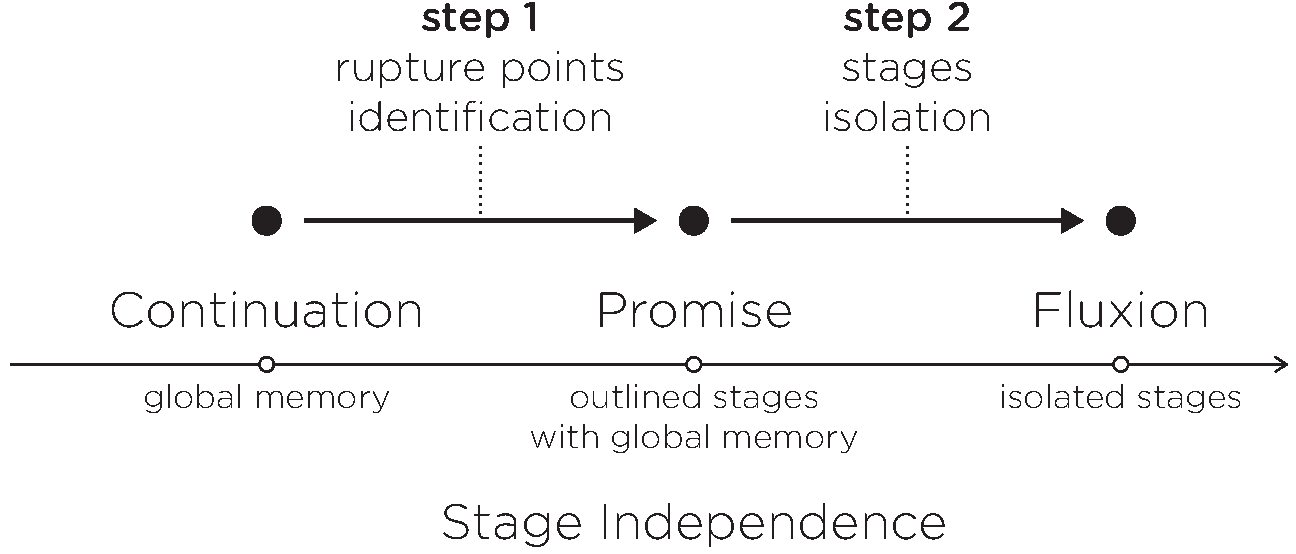
\includegraphics[width=0.7\textwidth]{../resources/roadmap.pdf}%
    \caption{Roadmap}%
    \label{fig:roadmap}%
  }%
\end{figure}

The first compiler focuses on the identification of simple chains of causality between continuations to transform these chains into Promises.
% the transformation from continuations to Promises.
% It focuses on the identification of the chains of causality in continuations.
However, promises are more expressive than the simple chaining of causal sequentiality.
% They force another control over the execution flow.
% According to the outcome of the operation, they call one function to continue the execution with the result, or another to handle errors.
% This conditional execution is indivisible from the Promise specification.
% Promises impose a convention on how to hand back the outcome of the deferred computation, while classic continuations leave this conditional execution to the developer.
Moreover, they impose a different convention than continuations on how to hand back the outcome and errors of the deferred computation.
This difference brings unnecessary complexity to the identification of chains.
To rule out this difference between continuations and Promises, before introducing the first compiler, section \ref{chapter5:due} introduces a simpler specification to Promise, called Due.

The second compiler detects all the chains of causality between continuations and encapsulate them in fluxions.
It isolates the fluxions when possible to allow the parallelism required for efficiency.
This second compilers is introduced in section \ref{chapter5:flx}.

\renewcommand{\glyph}{\iconfont{\XeTeXglyph287}}
\chapter{Implementations} \label{chapter5}
\minitoc
\eject
The transformation allowed by the equivalence from an event-driven program into a distributed network of fluxions is implemented incrementally into two compilers, as presented in figure \ref{fig:roadmap}.
Each compilers is divided into two steps, the identification of the rupture points separating the stages of the pipeline, and the isolation of these stages.
% This chapter presents the technical implementations of these two steps in the transformation from the event-driven execution model to the pipeline architecture
% , the transformation described in the previous chapter was implemented incrementally in two compilers.

\begin{figure}[h!]%
  \textfig{%
    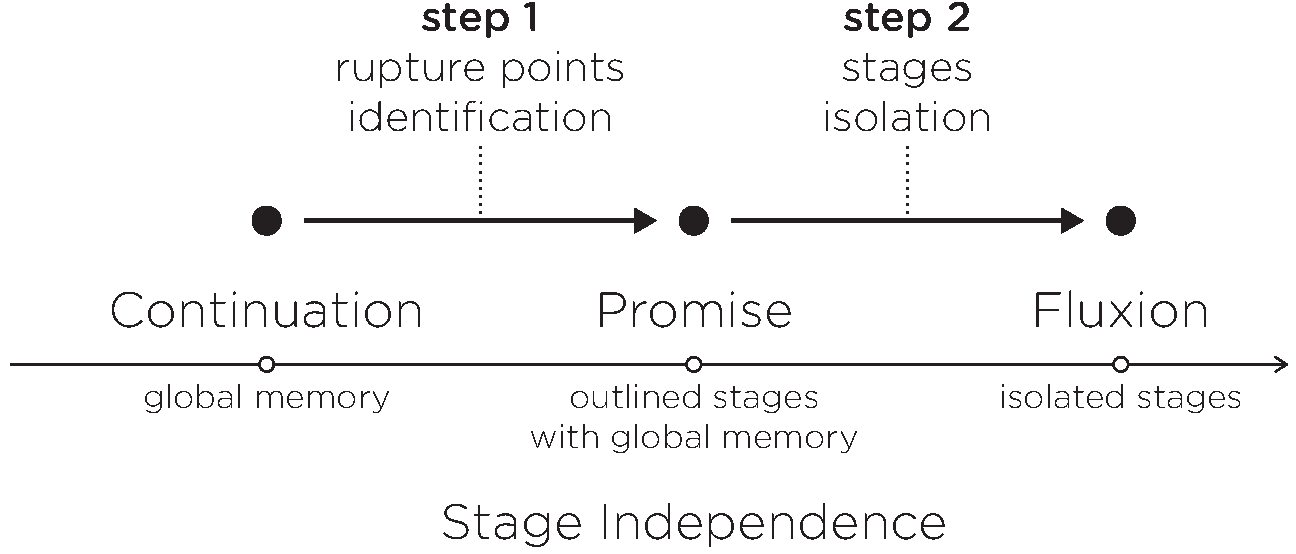
\includegraphics[width=0.7\textwidth]{../resources/roadmap.pdf}%
    \caption{Roadmap}%
    \label{fig:roadmap}%
  }%
\end{figure}

The first compiler focuses on the identification of simple chains of causality between continuations to transform these chains into Promises.
% the transformation from continuations to Promises.
% It focuses on the identification of the chains of causality in continuations.
However, promises are more expressive than the simple chaining of causal sequentiality.
% They force another control over the execution flow.
% According to the outcome of the operation, they call one function to continue the execution with the result, or another to handle errors.
% This conditional execution is indivisible from the Promise specification.
% Promises impose a convention on how to hand back the outcome of the deferred computation, while classic continuations leave this conditional execution to the developer.
Moreover, they impose a different convention than continuations on how to hand back the outcome and errors of the deferred computation.
This difference brings unnecessary complexity to the identification of chains.
To rule out this difference between continuations and Promises, before introducing the first compiler, section \ref{chapter5:due} introduces a simpler specification to Promise, called Due.

The second compiler detects all the chains of causality between continuations and encapsulate them in fluxions.
It isolates the fluxions when possible to allow the parallelism required for efficiency.
This second compilers is introduced in section \ref{chapter5:flx}.

\renewcommand{\glyph}{\iconfont{\XeTeXglyph287}}
\chapter{Implementations} \label{chapter5}
\minitoc
\eject
The transformation allowed by the equivalence from an event-driven program into a distributed network of fluxions is implemented incrementally into two compilers, as presented in figure \ref{fig:roadmap}.
Each compilers is divided into two steps, the identification of the rupture points separating the stages of the pipeline, and the isolation of these stages.
% This chapter presents the technical implementations of these two steps in the transformation from the event-driven execution model to the pipeline architecture
% , the transformation described in the previous chapter was implemented incrementally in two compilers.

\begin{figure}[h!]%
  \textfig{%
    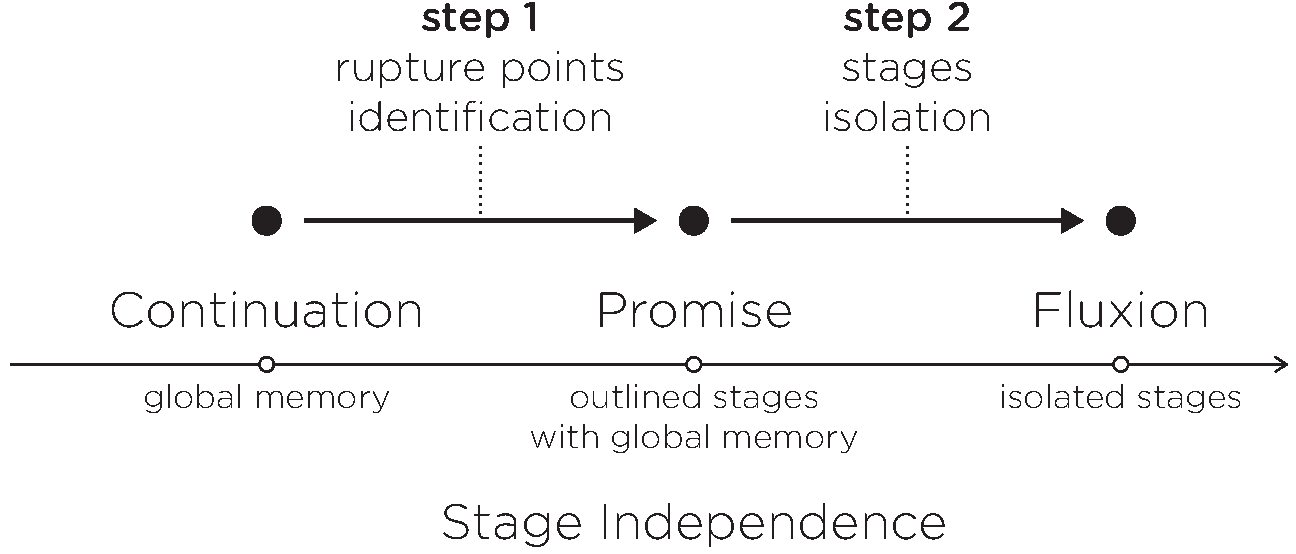
\includegraphics[width=0.7\textwidth]{../resources/roadmap.pdf}%
    \caption{Roadmap}%
    \label{fig:roadmap}%
  }%
\end{figure}

The first compiler focuses on the identification of simple chains of causality between continuations to transform these chains into Promises.
% the transformation from continuations to Promises.
% It focuses on the identification of the chains of causality in continuations.
However, promises are more expressive than the simple chaining of causal sequentiality.
% They force another control over the execution flow.
% According to the outcome of the operation, they call one function to continue the execution with the result, or another to handle errors.
% This conditional execution is indivisible from the Promise specification.
% Promises impose a convention on how to hand back the outcome of the deferred computation, while classic continuations leave this conditional execution to the developer.
Moreover, they impose a different convention than continuations on how to hand back the outcome and errors of the deferred computation.
This difference brings unnecessary complexity to the identification of chains.
To rule out this difference between continuations and Promises, before introducing the first compiler, section \ref{chapter5:due} introduces a simpler specification to Promise, called Due.

The second compiler detects all the chains of causality between continuations and encapsulate them in fluxions.
It isolates the fluxions when possible to allow the parallelism required for efficiency.
This second compilers is introduced in section \ref{chapter5:flx}.

\input{05-implementation/Due/main}
\input{05-implementation/Flx/main}
% \input{05-implementation/Evaluation}

\renewcommand{\glyph}{\iconfont{\XeTeXglyph287}}
\chapter{Implementations} \label{chapter5}
\minitoc
\eject
The transformation allowed by the equivalence from an event-driven program into a distributed network of fluxions is implemented incrementally into two compilers, as presented in figure \ref{fig:roadmap}.
Each compilers is divided into two steps, the identification of the rupture points separating the stages of the pipeline, and the isolation of these stages.
% This chapter presents the technical implementations of these two steps in the transformation from the event-driven execution model to the pipeline architecture
% , the transformation described in the previous chapter was implemented incrementally in two compilers.

\begin{figure}[h!]%
  \textfig{%
    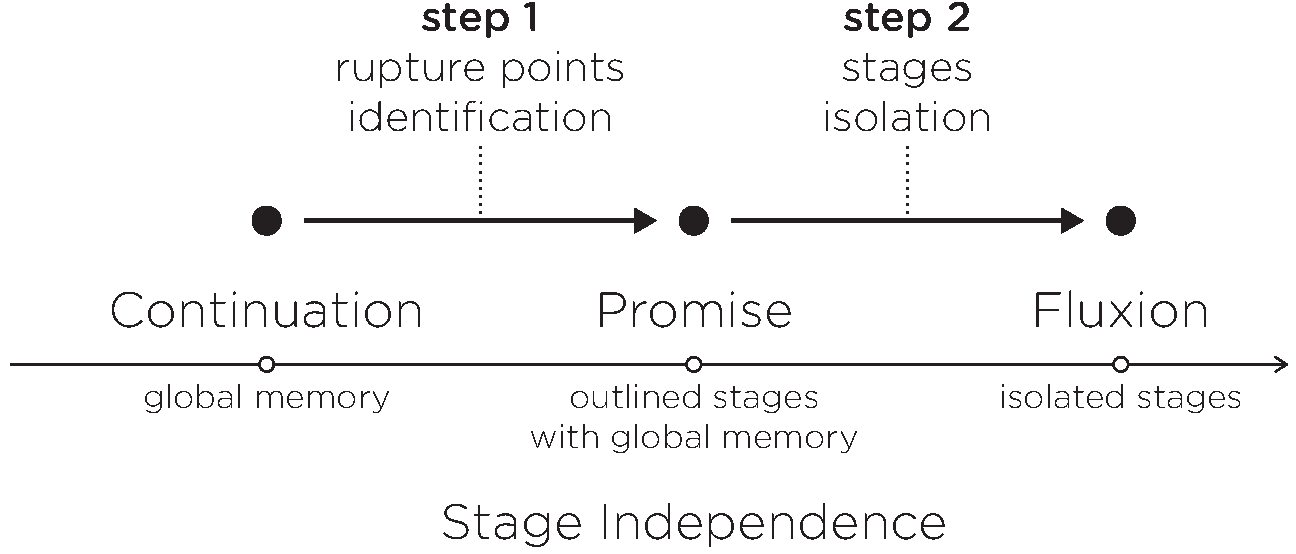
\includegraphics[width=0.7\textwidth]{../resources/roadmap.pdf}%
    \caption{Roadmap}%
    \label{fig:roadmap}%
  }%
\end{figure}

The first compiler focuses on the identification of simple chains of causality between continuations to transform these chains into Promises.
% the transformation from continuations to Promises.
% It focuses on the identification of the chains of causality in continuations.
However, promises are more expressive than the simple chaining of causal sequentiality.
% They force another control over the execution flow.
% According to the outcome of the operation, they call one function to continue the execution with the result, or another to handle errors.
% This conditional execution is indivisible from the Promise specification.
% Promises impose a convention on how to hand back the outcome of the deferred computation, while classic continuations leave this conditional execution to the developer.
Moreover, they impose a different convention than continuations on how to hand back the outcome and errors of the deferred computation.
This difference brings unnecessary complexity to the identification of chains.
To rule out this difference between continuations and Promises, before introducing the first compiler, section \ref{chapter5:due} introduces a simpler specification to Promise, called Due.

The second compiler detects all the chains of causality between continuations and encapsulate them in fluxions.
It isolates the fluxions when possible to allow the parallelism required for efficiency.
This second compilers is introduced in section \ref{chapter5:flx}.

\input{05-implementation/Due/main}
\input{05-implementation/Flx/main}
% \input{05-implementation/Evaluation}

% \subsection{Real test case} \label{chapter5:flx:evaluation}

The compiler is tested on a real application, gifsockets-server\ftnt{https://github.com/twolfson/gifsockets-server}.
This test proves the possibility for an application to be compiled into a network of independent parts.
It shows the current limitations of this isolation and the modifications needed on the application to circumvent them.

\begin{code}[js, caption={Simplified version of gifsockets-server},label={lst:gifsocket}]
var express = require('express'),
    app = express(),
    routes = require('gifsockets-middleware'), //@\label{lst:gifsocket:gif-mw}@
    getRawBody = require('raw-body');

function bodyParser(limit) { //@\label{lst:gifsocket:bodyParser}@
  return function saveBody(req, res, next) { //@\label{lst:gifsocket:saveBody}@
    getRawBody(req, { //@\label{lst:gifsocket:getRawBody}@
      expected: req.headers['content-length'],
      limit: limit
    }, function (err, buffer) { //@\label{lst:gifsocket:callback}@
      req.body = buffer;
      next(); //@\label{lst:gifsocket:next}@
    });
  };
}

app.post('/image/text', bodyParser(1 * 1024 * 1024), routes.writeTextToImages); //@\label{lst:gifsocket:app.post}@
app.listen(8000);
\end{code}

This application, simplified in listing \ref{lst:gifsocket}, is a real-time chat using gif-based communication channels.
It was selected from the evaluation set of the Due compiler because it is simple enough to illustrate this evaluation.
% \cite{Brodu2015}
%  from the \texttt{npm} registry because it depends on \texttt{express}, it is tested, working, and simple enough to illustrate this evaluation.
The server transforms the received text into a gif frame, and pushes it back to a never-ending gif to be displayed on the client.

On line \ref{lst:gifsocket:app.post}, the application registers two functions to process the requests received on the url \texttt{/image/text}.
The closure \texttt{saveBody}, line \ref{lst:gifsocket:saveBody}, returned by \texttt{bodyParser}, line \ref{lst:gifsocket:bodyParser}, and the method \texttt{routes.write\-Text\-To\-Images} from the external module \texttt{gifsockets-\-middleware}, line \ref{lst:gifsocket:gif-mw}.
The closure \texttt{saveBody} calls the asynchronous function \texttt{getRawBody} to get the request body.
Its callback handles the errors, and calls \texttt{next} to continue processing the request with the next function, \texttt{routes.write\-Text\-To\-Images}.

\subsubsection{Compilation} \label{chapter5:flx:evaluation:compilation}

% We compile this application with the compiler
The compilation result is in listing \ref{lst:flx-gifsocket}.
The function call \texttt{app.post}, line \ref{lst:gifsocket:app.post}, is a rupture point.
However, its callbacks, \texttt{bodyParser} and \texttt{routes.write\-Text\-To\-Images} are not declared \textit{in situ}.
They are evaluated as functions only at runtime.
As precised previously, the compiler discards these callbacks to avoid altering the semantic. % by moving or modifying their definition.
% For this reason, the compiler ignores this rupture point, to avoid interfering with the evaluation.

\begin{code}[flx, caption={Compilation result of gifsockets-server},label={lst:flx-gifsocket}]
flx main & express {req}
>> anonymous_1000 [req, next]
  var express = require('express'),
      app = express(),
      routes = require('gifsockets-middleware'), //@\label{lst:flx-gifsocket:gif-mw}@
      getRawBody = require('raw-body');

  function bodyParser(limit) { //@\label{lst:flx-gifsocket:bodyParser}@
    return function saveBody(req, res, next) { //@\label{lst:flx-gifsocket:saveBody}@
      getRawBody(req, { //@\label{lst:flx-gifsocket:getRawBody}@
        expected: req.headers['content-length'], //@\label{lst:flx-gifsocket:req.headers}@
        limit: limit
      }, >> anonymous_1000 [req, next]);
    };
  }

  app.post('/image/text', bodyParser(1 * 1024 * 1024), routes.writeTextToImages); //@\label{lst:flx-gifsocket:app.post}@
  app.listen(8000);

flx anonymous_1000
-> null
  function (err, buffer) { //@\label{lst:flx-gifsocket:callback}@
    req.body = buffer; //@\label{lst:flx-gifsocket:buffer}@
    next(); //@\label{lst:flx-gifsocket:next}@
  }
\end{code}

The compiler detects a rupture point : the function \texttt{get\-Raw\-Body} and its anonymous callback, line \ref{lst:gifsocket:callback}.
It encapsulates this callback in a fluxion named \texttt{anony\-mous\_\-1000}.
The callback is replaced with a stream placeholder to send the message stream to this downstream fluxion.
The variables \texttt{req} and \texttt{next} are appended to this message stream, to propagate their value from the \texttt{main} fluxion to the \texttt{anony\-mous\_\-1000} fluxion.

When \texttt{anony\-mous\_\-1000} is not isolated from the \texttt{main} fluxion, as if they belong to the same group, the compilation result works as expected.
The variables used in the fluxion, \texttt{req} and \texttt{next}, are still shared between the two fluxions.
In this situation fluxions are quite similar to Dues regarding memory shareing.
Our goal is to isolate the two fluxions, to be able to safely parallelize their executions.

\subsubsection{Isolation} \label{chapter5:flx:evaluation:isolation}

In listing \ref{lst:flx-gifsocket}, the fluxion \texttt{anony\-mous\_\-1000} modifies the object \texttt{req}, line \ref{lst:flx-gifsocket:buffer}, to store the text of the received request, and it calls \texttt{next} to continue the execution, line \ref{lst:flx-gifsocket:next}.
\texttt{req} is an alias to a memory location used in multiple palces in code.
Therefore, these operations produce side-effects that should propagate in the whole application, but the isolation prevents this propagation.
Isolating the fluxion \texttt{anony\-mous\_\-1000} produces runtime exceptions.
The next paragraph details how this situation is handled to allow the application to be parallelized.

\paragraph{Variable \texttt{req}}

The variable \texttt{req} is read in fluxion \texttt{main}, lines \ref{lst:flx-gifsocket:getRawBody} and \ref{lst:flx-gifsocket:req.headers}.
Then its property \texttt{body} is associated to \texttt{buffer} in fluxion \texttt{anony\-mous\_\-1000}, line \ref{lst:flx-gifsocket:buffer}.
The compiler is unable to identify the aliases of this variable. % further usages.
However, the side effect resulting from this association impacts a variable in the scope of the next callback, \texttt{routes.write\-Text\-To\-Images}.
In this test case, the application is modified manually to explicitly propagate this side-effect to the next callback through the function \texttt{next}.
The modifications of this function are explained further in the next paragraph.

\paragraph{Closure \texttt{next}}

The function \texttt{next} is a closure provided by the \texttt{express} \texttt{Router} to continue the execution with the next function to handle the client request.
Because it indirectly relies on the variable \texttt{req}, it is impossible to isolate its execution with the \texttt{anony\-mous\_\-1000} fluxion.
Instead, we modify \texttt{express}, so as to be compatible with the fluxional execution model.
We explain the modifications below.

\begin{code}[flx, caption={Simplified modification on the compiled result},label={lst:mflx-gifsocket}]
flx anonymous_1000
-> express_dispatcher
  function (err, buffer) { //@\label{lst:mflx-gifsocket:callback}@
    req.body = buffer; //@\label{lst:mflx-gifsocket:buffer}@
    next_placeholder(req, -> express_dispatcher); //@\label{lst:mflx-gifsocket:next-placeholder}@
  }

flx express_dispatcher & express {req} //@\label{lst:mflx-gifsocket:express-dispatcher}@
-> null
  function (modified_req) {
    merge(req, modified_req);
    next(); //@\label{lst:mflx-gifsocket:next}@
  }
\end{code}

In listing \ref{lst:gifsocket}, the function \texttt{next} is a continuation allowing the anonymous callback, line \ref{lst:gifsocket:callback}, to call the next function to handle the request.
To isolate the anonymous callback into \texttt{anonymous\_\-1000}, \texttt{next} is replaced by a rupture point.
This replacement is illustrated in listing \ref{lst:mflx-gifsocket}.
The \texttt{express} \texttt{Router} registers a fluxion named \texttt{express\_\-dispatcher}, line \ref{lst:mflx-gifsocket:express-dispatcher}, to continue the execution after the fluxion \texttt{anony\-mous\_\-1000}.
This fluxion is in the same group \texttt{express} as the \texttt{main} fluxion, hence it has access to the original variable \texttt{req}, and to the original function \texttt{next}.
The call to the original \texttt{next} function is replaced by a placeholder to push the stream to the fluxion \texttt{express\_\-dispatcher}, line \ref{lst:mflx-gifsocket:next-placeholder}.
The fluxion \texttt{express\_\-dispatcher} receives the stream from the upstream fluxion \texttt{anony\-mous\_\-1000}, merges back the modification in the variable \texttt{req} to propagate the side effects, and finally calls the original function \texttt{next} to continue the execution, line \ref{lst:mflx-gifsocket:next}.

After the modifications detailed above, the server works as expected.
The isolated fluxion correctly receives, and returns its serialized messages.
The client successfully receives a gif frame containing the text.



\subsection{Limitations}

The static analysis used for this compiler presents some limitations.
It is unable to analyze code with dynamic behaviors.
Higher-order programming leads to more productivity partly beacuse it rely on such dynamic behavior to extend expressivity.
Precisely, it allows more levels of indirections.

\subsubsection{Levels of Indirections}

The indirection is an abstraction between the value, and its manipulation.
In listing \ref{lst:indirection}, the variables \texttt{a} and \texttt{b} point both to the same memory object.
The function \texttt{fn} introduces a level of indirection between the real object \texttt{a} and its manipulation handle, \texttt{b};
% Actually, the variable \texttt{a} already introduces a level of indirection between the real object and the handle \texttt{a}.

\begin{code}[js,
  caption={One level of Indirection},
  label={lst:indirection}]
var a = {
      // an object;
    };

fn(b) {
  // modify b;
}

fn(a);
\end{code}

\subsubsection{Uncertainties}

The indirection is trivial to resolve in listing \ref{lst:indirection}.
It only needs to have access to the definition of \texttt{a} and of \texttt{fn}.
%A very simple static analysis could resolve it.
However, in listing \ref{lst:indirections}, the array \texttt{handlers} introduces a new level of indirection.
The static analysis now needs to have access to the definition of \texttt{i} and of the \texttt{handlers}.
If this definition is provided by an external input, it is not available statically, hence, it adds an uncertainty during the analysis. 

\begin{code}[js,
  caption={Two levels of indirection},
  label={lst:indirections}]
var a = {
      // an object;
    },
    handlers = [
      // definition of fn handlers;
    ],
    i = ?;

handlers[i](a);
handlers[i+1](a);
\end{code}

These examples are extremely simplified.
A real application contains enough indirections for the static analysis to be overwhelmed by uncertainties, and to be unable to resolve the variables.
If a variable is left unresolved, it is impossible to assure its scope and its aliases.
Therefore, the compiler is unable to isolate it into a fluxion, or to distribute its modification by messages.

Moreover, it leads the compiler to ignore the rupture points not defined \textit{in situ}, because their modifications could impact the semantic.
The reason for this precaution, is that the compiler is unable to assure where the function is used, and the scope of its variables.
Therefore, it is unable to assure that the modification will conserve the semantic.

\subsubsection{Dynamic Resolution}

In a web application, this variable \texttt{i} might be part of the user request, which is available only at runtime.
It eventually introduces an uncertainty.

This dynamic resolution of variables is precisely what increase expressiveness.
Trying to resolve them statically is equivalent to restrict expressiveness.
No static analysis can overstep these limitations.
Only a dynamic analysis could analysis the resolved indirections during run time to overstep these limitations correctly.




\renewcommand{\glyph}{\iconfont{\XeTeXglyph287}}
\chapter{Implementations} \label{chapter5}
\minitoc
\eject
The transformation allowed by the equivalence from an event-driven program into a distributed network of fluxions is implemented incrementally into two compilers, as presented in figure \ref{fig:roadmap}.
Each compilers is divided into two steps, the identification of the rupture points separating the stages of the pipeline, and the isolation of these stages.
% This chapter presents the technical implementations of these two steps in the transformation from the event-driven execution model to the pipeline architecture
% , the transformation described in the previous chapter was implemented incrementally in two compilers.

\begin{figure}[h!]%
  \textfig{%
    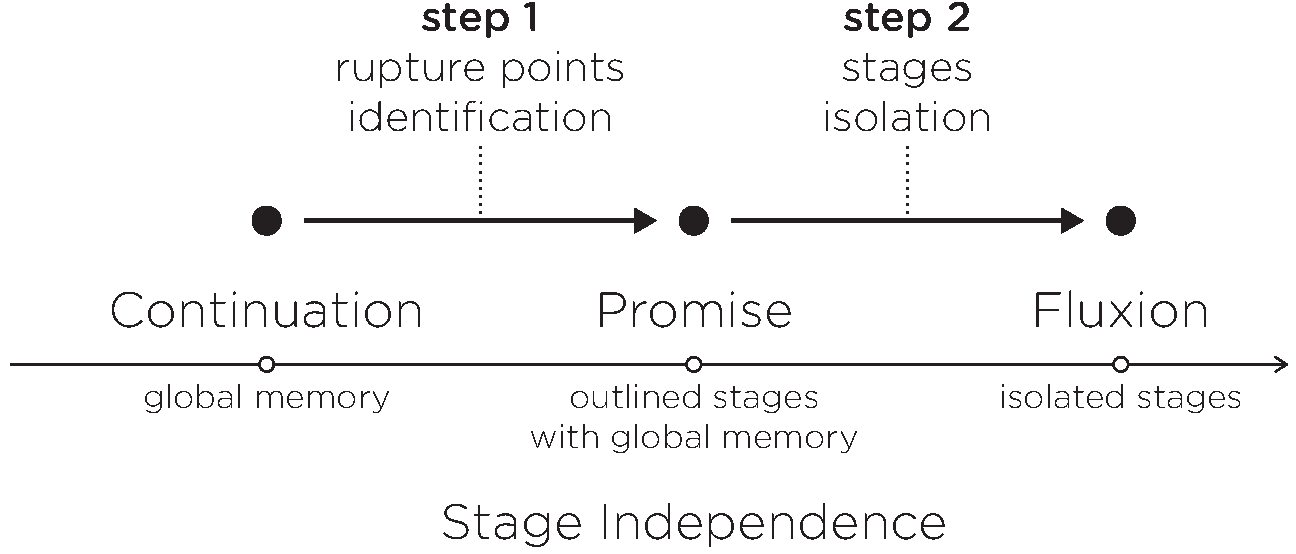
\includegraphics[width=0.7\textwidth]{../resources/roadmap.pdf}%
    \caption{Roadmap}%
    \label{fig:roadmap}%
  }%
\end{figure}

The first compiler focuses on the identification of simple chains of causality between continuations to transform these chains into Promises.
% the transformation from continuations to Promises.
% It focuses on the identification of the chains of causality in continuations.
However, promises are more expressive than the simple chaining of causal sequentiality.
% They force another control over the execution flow.
% According to the outcome of the operation, they call one function to continue the execution with the result, or another to handle errors.
% This conditional execution is indivisible from the Promise specification.
% Promises impose a convention on how to hand back the outcome of the deferred computation, while classic continuations leave this conditional execution to the developer.
Moreover, they impose a different convention than continuations on how to hand back the outcome and errors of the deferred computation.
This difference brings unnecessary complexity to the identification of chains.
To rule out this difference between continuations and Promises, before introducing the first compiler, section \ref{chapter5:due} introduces a simpler specification to Promise, called Due.

The second compiler detects all the chains of causality between continuations and encapsulate them in fluxions.
It isolates the fluxions when possible to allow the parallelism required for efficiency.
This second compilers is introduced in section \ref{chapter5:flx}.

\renewcommand{\glyph}{\iconfont{\XeTeXglyph287}}
\chapter{Implementations} \label{chapter5}
\minitoc
\eject
The transformation allowed by the equivalence from an event-driven program into a distributed network of fluxions is implemented incrementally into two compilers, as presented in figure \ref{fig:roadmap}.
Each compilers is divided into two steps, the identification of the rupture points separating the stages of the pipeline, and the isolation of these stages.
% This chapter presents the technical implementations of these two steps in the transformation from the event-driven execution model to the pipeline architecture
% , the transformation described in the previous chapter was implemented incrementally in two compilers.

\begin{figure}[h!]%
  \textfig{%
    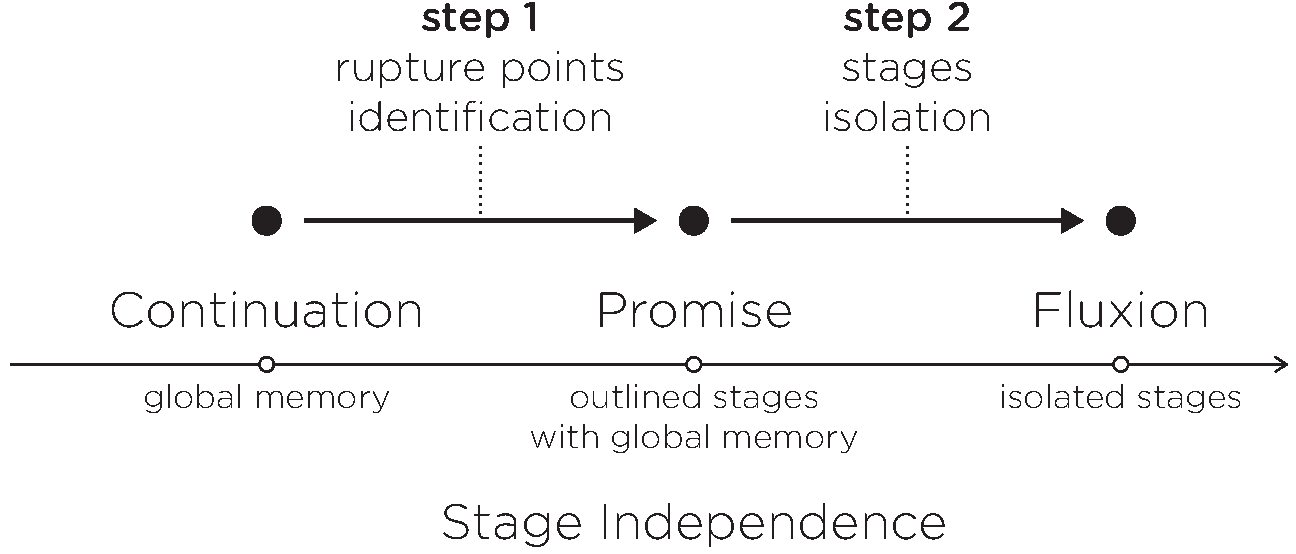
\includegraphics[width=0.7\textwidth]{../resources/roadmap.pdf}%
    \caption{Roadmap}%
    \label{fig:roadmap}%
  }%
\end{figure}

The first compiler focuses on the identification of simple chains of causality between continuations to transform these chains into Promises.
% the transformation from continuations to Promises.
% It focuses on the identification of the chains of causality in continuations.
However, promises are more expressive than the simple chaining of causal sequentiality.
% They force another control over the execution flow.
% According to the outcome of the operation, they call one function to continue the execution with the result, or another to handle errors.
% This conditional execution is indivisible from the Promise specification.
% Promises impose a convention on how to hand back the outcome of the deferred computation, while classic continuations leave this conditional execution to the developer.
Moreover, they impose a different convention than continuations on how to hand back the outcome and errors of the deferred computation.
This difference brings unnecessary complexity to the identification of chains.
To rule out this difference between continuations and Promises, before introducing the first compiler, section \ref{chapter5:due} introduces a simpler specification to Promise, called Due.

The second compiler detects all the chains of causality between continuations and encapsulate them in fluxions.
It isolates the fluxions when possible to allow the parallelism required for efficiency.
This second compilers is introduced in section \ref{chapter5:flx}.

\input{05-implementation/Due/main}
\input{05-implementation/Flx/main}
% \input{05-implementation/Evaluation}

\renewcommand{\glyph}{\iconfont{\XeTeXglyph287}}
\chapter{Implementations} \label{chapter5}
\minitoc
\eject
The transformation allowed by the equivalence from an event-driven program into a distributed network of fluxions is implemented incrementally into two compilers, as presented in figure \ref{fig:roadmap}.
Each compilers is divided into two steps, the identification of the rupture points separating the stages of the pipeline, and the isolation of these stages.
% This chapter presents the technical implementations of these two steps in the transformation from the event-driven execution model to the pipeline architecture
% , the transformation described in the previous chapter was implemented incrementally in two compilers.

\begin{figure}[h!]%
  \textfig{%
    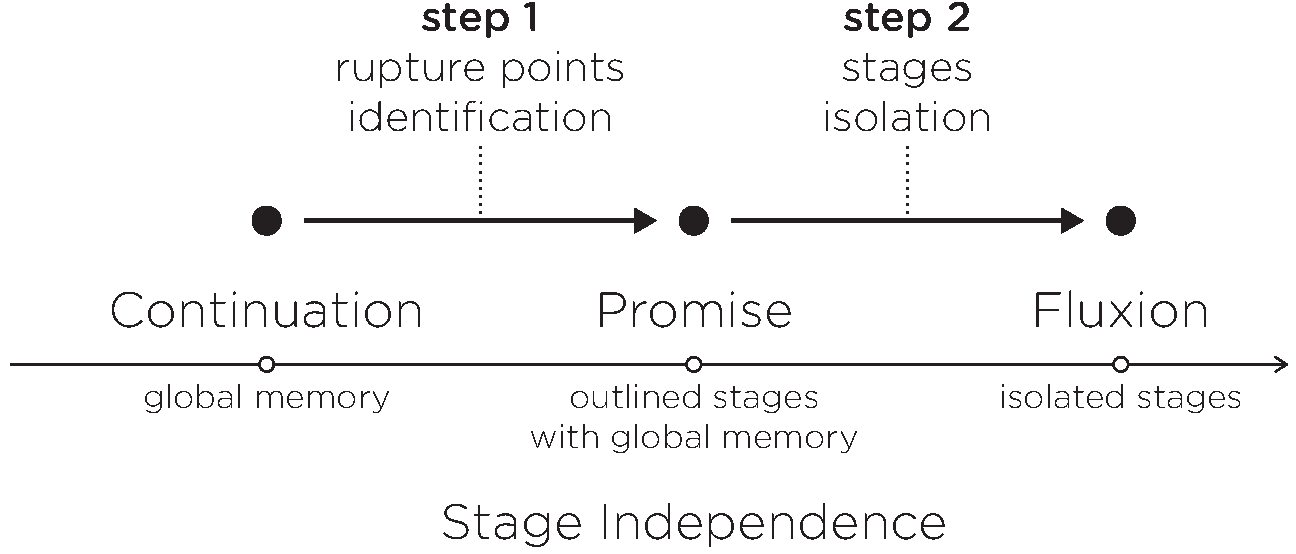
\includegraphics[width=0.7\textwidth]{../resources/roadmap.pdf}%
    \caption{Roadmap}%
    \label{fig:roadmap}%
  }%
\end{figure}

The first compiler focuses on the identification of simple chains of causality between continuations to transform these chains into Promises.
% the transformation from continuations to Promises.
% It focuses on the identification of the chains of causality in continuations.
However, promises are more expressive than the simple chaining of causal sequentiality.
% They force another control over the execution flow.
% According to the outcome of the operation, they call one function to continue the execution with the result, or another to handle errors.
% This conditional execution is indivisible from the Promise specification.
% Promises impose a convention on how to hand back the outcome of the deferred computation, while classic continuations leave this conditional execution to the developer.
Moreover, they impose a different convention than continuations on how to hand back the outcome and errors of the deferred computation.
This difference brings unnecessary complexity to the identification of chains.
To rule out this difference between continuations and Promises, before introducing the first compiler, section \ref{chapter5:due} introduces a simpler specification to Promise, called Due.

The second compiler detects all the chains of causality between continuations and encapsulate them in fluxions.
It isolates the fluxions when possible to allow the parallelism required for efficiency.
This second compilers is introduced in section \ref{chapter5:flx}.

\input{05-implementation/Due/main}
\input{05-implementation/Flx/main}
% \input{05-implementation/Evaluation}

% \subsection{Real test case} \label{chapter5:flx:evaluation}

The compiler is tested on a real application, gifsockets-server\ftnt{https://github.com/twolfson/gifsockets-server}.
This test proves the possibility for an application to be compiled into a network of independent parts.
It shows the current limitations of this isolation and the modifications needed on the application to circumvent them.

\begin{code}[js, caption={Simplified version of gifsockets-server},label={lst:gifsocket}]
var express = require('express'),
    app = express(),
    routes = require('gifsockets-middleware'), //@\label{lst:gifsocket:gif-mw}@
    getRawBody = require('raw-body');

function bodyParser(limit) { //@\label{lst:gifsocket:bodyParser}@
  return function saveBody(req, res, next) { //@\label{lst:gifsocket:saveBody}@
    getRawBody(req, { //@\label{lst:gifsocket:getRawBody}@
      expected: req.headers['content-length'],
      limit: limit
    }, function (err, buffer) { //@\label{lst:gifsocket:callback}@
      req.body = buffer;
      next(); //@\label{lst:gifsocket:next}@
    });
  };
}

app.post('/image/text', bodyParser(1 * 1024 * 1024), routes.writeTextToImages); //@\label{lst:gifsocket:app.post}@
app.listen(8000);
\end{code}

This application, simplified in listing \ref{lst:gifsocket}, is a real-time chat using gif-based communication channels.
It was selected from the evaluation set of the Due compiler because it is simple enough to illustrate this evaluation.
% \cite{Brodu2015}
%  from the \texttt{npm} registry because it depends on \texttt{express}, it is tested, working, and simple enough to illustrate this evaluation.
The server transforms the received text into a gif frame, and pushes it back to a never-ending gif to be displayed on the client.

On line \ref{lst:gifsocket:app.post}, the application registers two functions to process the requests received on the url \texttt{/image/text}.
The closure \texttt{saveBody}, line \ref{lst:gifsocket:saveBody}, returned by \texttt{bodyParser}, line \ref{lst:gifsocket:bodyParser}, and the method \texttt{routes.write\-Text\-To\-Images} from the external module \texttt{gifsockets-\-middleware}, line \ref{lst:gifsocket:gif-mw}.
The closure \texttt{saveBody} calls the asynchronous function \texttt{getRawBody} to get the request body.
Its callback handles the errors, and calls \texttt{next} to continue processing the request with the next function, \texttt{routes.write\-Text\-To\-Images}.

\subsubsection{Compilation} \label{chapter5:flx:evaluation:compilation}

% We compile this application with the compiler
The compilation result is in listing \ref{lst:flx-gifsocket}.
The function call \texttt{app.post}, line \ref{lst:gifsocket:app.post}, is a rupture point.
However, its callbacks, \texttt{bodyParser} and \texttt{routes.write\-Text\-To\-Images} are not declared \textit{in situ}.
They are evaluated as functions only at runtime.
As precised previously, the compiler discards these callbacks to avoid altering the semantic. % by moving or modifying their definition.
% For this reason, the compiler ignores this rupture point, to avoid interfering with the evaluation.

\begin{code}[flx, caption={Compilation result of gifsockets-server},label={lst:flx-gifsocket}]
flx main & express {req}
>> anonymous_1000 [req, next]
  var express = require('express'),
      app = express(),
      routes = require('gifsockets-middleware'), //@\label{lst:flx-gifsocket:gif-mw}@
      getRawBody = require('raw-body');

  function bodyParser(limit) { //@\label{lst:flx-gifsocket:bodyParser}@
    return function saveBody(req, res, next) { //@\label{lst:flx-gifsocket:saveBody}@
      getRawBody(req, { //@\label{lst:flx-gifsocket:getRawBody}@
        expected: req.headers['content-length'], //@\label{lst:flx-gifsocket:req.headers}@
        limit: limit
      }, >> anonymous_1000 [req, next]);
    };
  }

  app.post('/image/text', bodyParser(1 * 1024 * 1024), routes.writeTextToImages); //@\label{lst:flx-gifsocket:app.post}@
  app.listen(8000);

flx anonymous_1000
-> null
  function (err, buffer) { //@\label{lst:flx-gifsocket:callback}@
    req.body = buffer; //@\label{lst:flx-gifsocket:buffer}@
    next(); //@\label{lst:flx-gifsocket:next}@
  }
\end{code}

The compiler detects a rupture point : the function \texttt{get\-Raw\-Body} and its anonymous callback, line \ref{lst:gifsocket:callback}.
It encapsulates this callback in a fluxion named \texttt{anony\-mous\_\-1000}.
The callback is replaced with a stream placeholder to send the message stream to this downstream fluxion.
The variables \texttt{req} and \texttt{next} are appended to this message stream, to propagate their value from the \texttt{main} fluxion to the \texttt{anony\-mous\_\-1000} fluxion.

When \texttt{anony\-mous\_\-1000} is not isolated from the \texttt{main} fluxion, as if they belong to the same group, the compilation result works as expected.
The variables used in the fluxion, \texttt{req} and \texttt{next}, are still shared between the two fluxions.
In this situation fluxions are quite similar to Dues regarding memory shareing.
Our goal is to isolate the two fluxions, to be able to safely parallelize their executions.

\subsubsection{Isolation} \label{chapter5:flx:evaluation:isolation}

In listing \ref{lst:flx-gifsocket}, the fluxion \texttt{anony\-mous\_\-1000} modifies the object \texttt{req}, line \ref{lst:flx-gifsocket:buffer}, to store the text of the received request, and it calls \texttt{next} to continue the execution, line \ref{lst:flx-gifsocket:next}.
\texttt{req} is an alias to a memory location used in multiple palces in code.
Therefore, these operations produce side-effects that should propagate in the whole application, but the isolation prevents this propagation.
Isolating the fluxion \texttt{anony\-mous\_\-1000} produces runtime exceptions.
The next paragraph details how this situation is handled to allow the application to be parallelized.

\paragraph{Variable \texttt{req}}

The variable \texttt{req} is read in fluxion \texttt{main}, lines \ref{lst:flx-gifsocket:getRawBody} and \ref{lst:flx-gifsocket:req.headers}.
Then its property \texttt{body} is associated to \texttt{buffer} in fluxion \texttt{anony\-mous\_\-1000}, line \ref{lst:flx-gifsocket:buffer}.
The compiler is unable to identify the aliases of this variable. % further usages.
However, the side effect resulting from this association impacts a variable in the scope of the next callback, \texttt{routes.write\-Text\-To\-Images}.
In this test case, the application is modified manually to explicitly propagate this side-effect to the next callback through the function \texttt{next}.
The modifications of this function are explained further in the next paragraph.

\paragraph{Closure \texttt{next}}

The function \texttt{next} is a closure provided by the \texttt{express} \texttt{Router} to continue the execution with the next function to handle the client request.
Because it indirectly relies on the variable \texttt{req}, it is impossible to isolate its execution with the \texttt{anony\-mous\_\-1000} fluxion.
Instead, we modify \texttt{express}, so as to be compatible with the fluxional execution model.
We explain the modifications below.

\begin{code}[flx, caption={Simplified modification on the compiled result},label={lst:mflx-gifsocket}]
flx anonymous_1000
-> express_dispatcher
  function (err, buffer) { //@\label{lst:mflx-gifsocket:callback}@
    req.body = buffer; //@\label{lst:mflx-gifsocket:buffer}@
    next_placeholder(req, -> express_dispatcher); //@\label{lst:mflx-gifsocket:next-placeholder}@
  }

flx express_dispatcher & express {req} //@\label{lst:mflx-gifsocket:express-dispatcher}@
-> null
  function (modified_req) {
    merge(req, modified_req);
    next(); //@\label{lst:mflx-gifsocket:next}@
  }
\end{code}

In listing \ref{lst:gifsocket}, the function \texttt{next} is a continuation allowing the anonymous callback, line \ref{lst:gifsocket:callback}, to call the next function to handle the request.
To isolate the anonymous callback into \texttt{anonymous\_\-1000}, \texttt{next} is replaced by a rupture point.
This replacement is illustrated in listing \ref{lst:mflx-gifsocket}.
The \texttt{express} \texttt{Router} registers a fluxion named \texttt{express\_\-dispatcher}, line \ref{lst:mflx-gifsocket:express-dispatcher}, to continue the execution after the fluxion \texttt{anony\-mous\_\-1000}.
This fluxion is in the same group \texttt{express} as the \texttt{main} fluxion, hence it has access to the original variable \texttt{req}, and to the original function \texttt{next}.
The call to the original \texttt{next} function is replaced by a placeholder to push the stream to the fluxion \texttt{express\_\-dispatcher}, line \ref{lst:mflx-gifsocket:next-placeholder}.
The fluxion \texttt{express\_\-dispatcher} receives the stream from the upstream fluxion \texttt{anony\-mous\_\-1000}, merges back the modification in the variable \texttt{req} to propagate the side effects, and finally calls the original function \texttt{next} to continue the execution, line \ref{lst:mflx-gifsocket:next}.

After the modifications detailed above, the server works as expected.
The isolated fluxion correctly receives, and returns its serialized messages.
The client successfully receives a gif frame containing the text.



\subsection{Limitations}

The static analysis used for this compiler presents some limitations.
It is unable to analyze code with dynamic behaviors.
Higher-order programming leads to more productivity partly beacuse it rely on such dynamic behavior to extend expressivity.
Precisely, it allows more levels of indirections.

\subsubsection{Levels of Indirections}

The indirection is an abstraction between the value, and its manipulation.
In listing \ref{lst:indirection}, the variables \texttt{a} and \texttt{b} point both to the same memory object.
The function \texttt{fn} introduces a level of indirection between the real object \texttt{a} and its manipulation handle, \texttt{b};
% Actually, the variable \texttt{a} already introduces a level of indirection between the real object and the handle \texttt{a}.

\begin{code}[js,
  caption={One level of Indirection},
  label={lst:indirection}]
var a = {
      // an object;
    };

fn(b) {
  // modify b;
}

fn(a);
\end{code}

\subsubsection{Uncertainties}

The indirection is trivial to resolve in listing \ref{lst:indirection}.
It only needs to have access to the definition of \texttt{a} and of \texttt{fn}.
%A very simple static analysis could resolve it.
However, in listing \ref{lst:indirections}, the array \texttt{handlers} introduces a new level of indirection.
The static analysis now needs to have access to the definition of \texttt{i} and of the \texttt{handlers}.
If this definition is provided by an external input, it is not available statically, hence, it adds an uncertainty during the analysis. 

\begin{code}[js,
  caption={Two levels of indirection},
  label={lst:indirections}]
var a = {
      // an object;
    },
    handlers = [
      // definition of fn handlers;
    ],
    i = ?;

handlers[i](a);
handlers[i+1](a);
\end{code}

These examples are extremely simplified.
A real application contains enough indirections for the static analysis to be overwhelmed by uncertainties, and to be unable to resolve the variables.
If a variable is left unresolved, it is impossible to assure its scope and its aliases.
Therefore, the compiler is unable to isolate it into a fluxion, or to distribute its modification by messages.

Moreover, it leads the compiler to ignore the rupture points not defined \textit{in situ}, because their modifications could impact the semantic.
The reason for this precaution, is that the compiler is unable to assure where the function is used, and the scope of its variables.
Therefore, it is unable to assure that the modification will conserve the semantic.

\subsubsection{Dynamic Resolution}

In a web application, this variable \texttt{i} might be part of the user request, which is available only at runtime.
It eventually introduces an uncertainty.

This dynamic resolution of variables is precisely what increase expressiveness.
Trying to resolve them statically is equivalent to restrict expressiveness.
No static analysis can overstep these limitations.
Only a dynamic analysis could analysis the resolved indirections during run time to overstep these limitations correctly.




% \subsection{Real test case} \label{chapter5:flx:evaluation}

The compiler is tested on a real application, gifsockets-server\ftnt{https://github.com/twolfson/gifsockets-server}.
This test proves the possibility for an application to be compiled into a network of independent parts.
It shows the current limitations of this isolation and the modifications needed on the application to circumvent them.

\begin{code}[js, caption={Simplified version of gifsockets-server},label={lst:gifsocket}]
var express = require('express'),
    app = express(),
    routes = require('gifsockets-middleware'), //@\label{lst:gifsocket:gif-mw}@
    getRawBody = require('raw-body');

function bodyParser(limit) { //@\label{lst:gifsocket:bodyParser}@
  return function saveBody(req, res, next) { //@\label{lst:gifsocket:saveBody}@
    getRawBody(req, { //@\label{lst:gifsocket:getRawBody}@
      expected: req.headers['content-length'],
      limit: limit
    }, function (err, buffer) { //@\label{lst:gifsocket:callback}@
      req.body = buffer;
      next(); //@\label{lst:gifsocket:next}@
    });
  };
}

app.post('/image/text', bodyParser(1 * 1024 * 1024), routes.writeTextToImages); //@\label{lst:gifsocket:app.post}@
app.listen(8000);
\end{code}

This application, simplified in listing \ref{lst:gifsocket}, is a real-time chat using gif-based communication channels.
It was selected from the evaluation set of the Due compiler because it is simple enough to illustrate this evaluation.
% \cite{Brodu2015}
%  from the \texttt{npm} registry because it depends on \texttt{express}, it is tested, working, and simple enough to illustrate this evaluation.
The server transforms the received text into a gif frame, and pushes it back to a never-ending gif to be displayed on the client.

On line \ref{lst:gifsocket:app.post}, the application registers two functions to process the requests received on the url \texttt{/image/text}.
The closure \texttt{saveBody}, line \ref{lst:gifsocket:saveBody}, returned by \texttt{bodyParser}, line \ref{lst:gifsocket:bodyParser}, and the method \texttt{routes.write\-Text\-To\-Images} from the external module \texttt{gifsockets-\-middleware}, line \ref{lst:gifsocket:gif-mw}.
The closure \texttt{saveBody} calls the asynchronous function \texttt{getRawBody} to get the request body.
Its callback handles the errors, and calls \texttt{next} to continue processing the request with the next function, \texttt{routes.write\-Text\-To\-Images}.

\subsubsection{Compilation} \label{chapter5:flx:evaluation:compilation}

% We compile this application with the compiler
The compilation result is in listing \ref{lst:flx-gifsocket}.
The function call \texttt{app.post}, line \ref{lst:gifsocket:app.post}, is a rupture point.
However, its callbacks, \texttt{bodyParser} and \texttt{routes.write\-Text\-To\-Images} are not declared \textit{in situ}.
They are evaluated as functions only at runtime.
As precised previously, the compiler discards these callbacks to avoid altering the semantic. % by moving or modifying their definition.
% For this reason, the compiler ignores this rupture point, to avoid interfering with the evaluation.

\begin{code}[flx, caption={Compilation result of gifsockets-server},label={lst:flx-gifsocket}]
flx main & express {req}
>> anonymous_1000 [req, next]
  var express = require('express'),
      app = express(),
      routes = require('gifsockets-middleware'), //@\label{lst:flx-gifsocket:gif-mw}@
      getRawBody = require('raw-body');

  function bodyParser(limit) { //@\label{lst:flx-gifsocket:bodyParser}@
    return function saveBody(req, res, next) { //@\label{lst:flx-gifsocket:saveBody}@
      getRawBody(req, { //@\label{lst:flx-gifsocket:getRawBody}@
        expected: req.headers['content-length'], //@\label{lst:flx-gifsocket:req.headers}@
        limit: limit
      }, >> anonymous_1000 [req, next]);
    };
  }

  app.post('/image/text', bodyParser(1 * 1024 * 1024), routes.writeTextToImages); //@\label{lst:flx-gifsocket:app.post}@
  app.listen(8000);

flx anonymous_1000
-> null
  function (err, buffer) { //@\label{lst:flx-gifsocket:callback}@
    req.body = buffer; //@\label{lst:flx-gifsocket:buffer}@
    next(); //@\label{lst:flx-gifsocket:next}@
  }
\end{code}

The compiler detects a rupture point : the function \texttt{get\-Raw\-Body} and its anonymous callback, line \ref{lst:gifsocket:callback}.
It encapsulates this callback in a fluxion named \texttt{anony\-mous\_\-1000}.
The callback is replaced with a stream placeholder to send the message stream to this downstream fluxion.
The variables \texttt{req} and \texttt{next} are appended to this message stream, to propagate their value from the \texttt{main} fluxion to the \texttt{anony\-mous\_\-1000} fluxion.

When \texttt{anony\-mous\_\-1000} is not isolated from the \texttt{main} fluxion, as if they belong to the same group, the compilation result works as expected.
The variables used in the fluxion, \texttt{req} and \texttt{next}, are still shared between the two fluxions.
In this situation fluxions are quite similar to Dues regarding memory shareing.
Our goal is to isolate the two fluxions, to be able to safely parallelize their executions.

\subsubsection{Isolation} \label{chapter5:flx:evaluation:isolation}

In listing \ref{lst:flx-gifsocket}, the fluxion \texttt{anony\-mous\_\-1000} modifies the object \texttt{req}, line \ref{lst:flx-gifsocket:buffer}, to store the text of the received request, and it calls \texttt{next} to continue the execution, line \ref{lst:flx-gifsocket:next}.
\texttt{req} is an alias to a memory location used in multiple palces in code.
Therefore, these operations produce side-effects that should propagate in the whole application, but the isolation prevents this propagation.
Isolating the fluxion \texttt{anony\-mous\_\-1000} produces runtime exceptions.
The next paragraph details how this situation is handled to allow the application to be parallelized.

\paragraph{Variable \texttt{req}}

The variable \texttt{req} is read in fluxion \texttt{main}, lines \ref{lst:flx-gifsocket:getRawBody} and \ref{lst:flx-gifsocket:req.headers}.
Then its property \texttt{body} is associated to \texttt{buffer} in fluxion \texttt{anony\-mous\_\-1000}, line \ref{lst:flx-gifsocket:buffer}.
The compiler is unable to identify the aliases of this variable. % further usages.
However, the side effect resulting from this association impacts a variable in the scope of the next callback, \texttt{routes.write\-Text\-To\-Images}.
In this test case, the application is modified manually to explicitly propagate this side-effect to the next callback through the function \texttt{next}.
The modifications of this function are explained further in the next paragraph.

\paragraph{Closure \texttt{next}}

The function \texttt{next} is a closure provided by the \texttt{express} \texttt{Router} to continue the execution with the next function to handle the client request.
Because it indirectly relies on the variable \texttt{req}, it is impossible to isolate its execution with the \texttt{anony\-mous\_\-1000} fluxion.
Instead, we modify \texttt{express}, so as to be compatible with the fluxional execution model.
We explain the modifications below.

\begin{code}[flx, caption={Simplified modification on the compiled result},label={lst:mflx-gifsocket}]
flx anonymous_1000
-> express_dispatcher
  function (err, buffer) { //@\label{lst:mflx-gifsocket:callback}@
    req.body = buffer; //@\label{lst:mflx-gifsocket:buffer}@
    next_placeholder(req, -> express_dispatcher); //@\label{lst:mflx-gifsocket:next-placeholder}@
  }

flx express_dispatcher & express {req} //@\label{lst:mflx-gifsocket:express-dispatcher}@
-> null
  function (modified_req) {
    merge(req, modified_req);
    next(); //@\label{lst:mflx-gifsocket:next}@
  }
\end{code}

In listing \ref{lst:gifsocket}, the function \texttt{next} is a continuation allowing the anonymous callback, line \ref{lst:gifsocket:callback}, to call the next function to handle the request.
To isolate the anonymous callback into \texttt{anonymous\_\-1000}, \texttt{next} is replaced by a rupture point.
This replacement is illustrated in listing \ref{lst:mflx-gifsocket}.
The \texttt{express} \texttt{Router} registers a fluxion named \texttt{express\_\-dispatcher}, line \ref{lst:mflx-gifsocket:express-dispatcher}, to continue the execution after the fluxion \texttt{anony\-mous\_\-1000}.
This fluxion is in the same group \texttt{express} as the \texttt{main} fluxion, hence it has access to the original variable \texttt{req}, and to the original function \texttt{next}.
The call to the original \texttt{next} function is replaced by a placeholder to push the stream to the fluxion \texttt{express\_\-dispatcher}, line \ref{lst:mflx-gifsocket:next-placeholder}.
The fluxion \texttt{express\_\-dispatcher} receives the stream from the upstream fluxion \texttt{anony\-mous\_\-1000}, merges back the modification in the variable \texttt{req} to propagate the side effects, and finally calls the original function \texttt{next} to continue the execution, line \ref{lst:mflx-gifsocket:next}.

After the modifications detailed above, the server works as expected.
The isolated fluxion correctly receives, and returns its serialized messages.
The client successfully receives a gif frame containing the text.



\subsection{Limitations}

The static analysis used for this compiler presents some limitations.
It is unable to analyze code with dynamic behaviors.
Higher-order programming leads to more productivity partly beacuse it rely on such dynamic behavior to extend expressivity.
Precisely, it allows more levels of indirections.

\subsubsection{Levels of Indirections}

The indirection is an abstraction between the value, and its manipulation.
In listing \ref{lst:indirection}, the variables \texttt{a} and \texttt{b} point both to the same memory object.
The function \texttt{fn} introduces a level of indirection between the real object \texttt{a} and its manipulation handle, \texttt{b};
% Actually, the variable \texttt{a} already introduces a level of indirection between the real object and the handle \texttt{a}.

\begin{code}[js,
  caption={One level of Indirection},
  label={lst:indirection}]
var a = {
      // an object;
    };

fn(b) {
  // modify b;
}

fn(a);
\end{code}

\subsubsection{Uncertainties}

The indirection is trivial to resolve in listing \ref{lst:indirection}.
It only needs to have access to the definition of \texttt{a} and of \texttt{fn}.
%A very simple static analysis could resolve it.
However, in listing \ref{lst:indirections}, the array \texttt{handlers} introduces a new level of indirection.
The static analysis now needs to have access to the definition of \texttt{i} and of the \texttt{handlers}.
If this definition is provided by an external input, it is not available statically, hence, it adds an uncertainty during the analysis. 

\begin{code}[js,
  caption={Two levels of indirection},
  label={lst:indirections}]
var a = {
      // an object;
    },
    handlers = [
      // definition of fn handlers;
    ],
    i = ?;

handlers[i](a);
handlers[i+1](a);
\end{code}

These examples are extremely simplified.
A real application contains enough indirections for the static analysis to be overwhelmed by uncertainties, and to be unable to resolve the variables.
If a variable is left unresolved, it is impossible to assure its scope and its aliases.
Therefore, the compiler is unable to isolate it into a fluxion, or to distribute its modification by messages.

Moreover, it leads the compiler to ignore the rupture points not defined \textit{in situ}, because their modifications could impact the semantic.
The reason for this precaution, is that the compiler is unable to assure where the function is used, and the scope of its variables.
Therefore, it is unable to assure that the modification will conserve the semantic.

\subsubsection{Dynamic Resolution}

In a web application, this variable \texttt{i} might be part of the user request, which is available only at runtime.
It eventually introduces an uncertainty.

This dynamic resolution of variables is precisely what increase expressiveness.
Trying to resolve them statically is equivalent to restrict expressiveness.
No static analysis can overstep these limitations.
Only a dynamic analysis could analysis the resolved indirections during run time to overstep these limitations correctly.




\renewcommand{\glyph}{\iconfont{\XeTeXglyph287}}
\chapter{Implementations} \label{chapter5}
\minitoc
\eject
The transformation allowed by the equivalence from an event-driven program into a distributed network of fluxions is implemented incrementally into two compilers, as presented in figure \ref{fig:roadmap}.
Each compilers is divided into two steps, the identification of the rupture points separating the stages of the pipeline, and the isolation of these stages.
% This chapter presents the technical implementations of these two steps in the transformation from the event-driven execution model to the pipeline architecture
% , the transformation described in the previous chapter was implemented incrementally in two compilers.

\begin{figure}[h!]%
  \textfig{%
    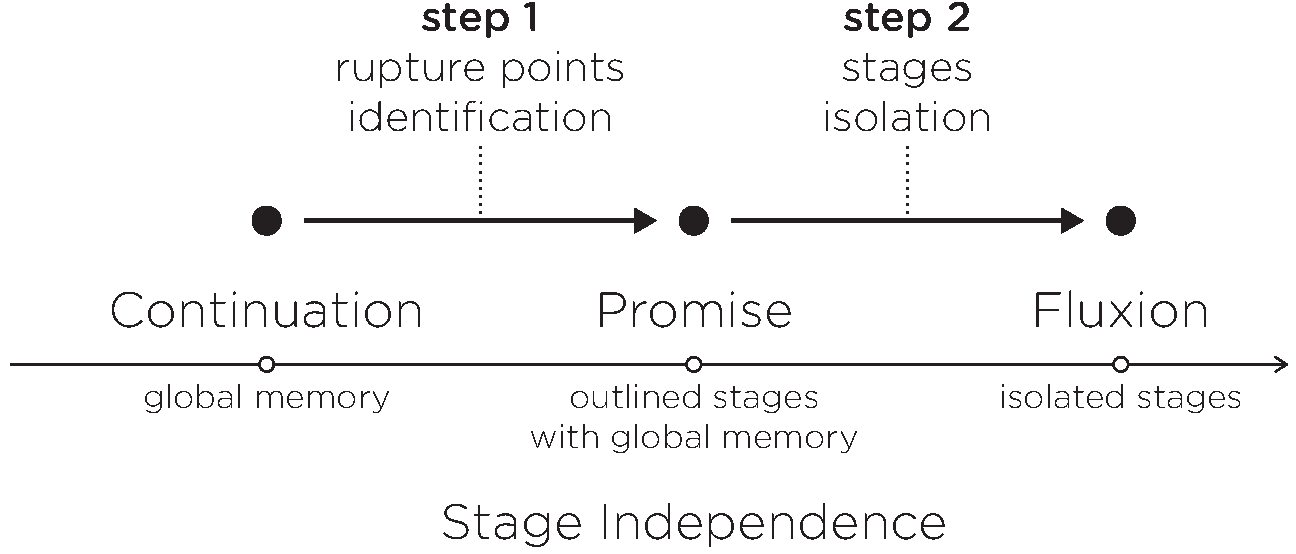
\includegraphics[width=0.7\textwidth]{../resources/roadmap.pdf}%
    \caption{Roadmap}%
    \label{fig:roadmap}%
  }%
\end{figure}

The first compiler focuses on the identification of simple chains of causality between continuations to transform these chains into Promises.
% the transformation from continuations to Promises.
% It focuses on the identification of the chains of causality in continuations.
However, promises are more expressive than the simple chaining of causal sequentiality.
% They force another control over the execution flow.
% According to the outcome of the operation, they call one function to continue the execution with the result, or another to handle errors.
% This conditional execution is indivisible from the Promise specification.
% Promises impose a convention on how to hand back the outcome of the deferred computation, while classic continuations leave this conditional execution to the developer.
Moreover, they impose a different convention than continuations on how to hand back the outcome and errors of the deferred computation.
This difference brings unnecessary complexity to the identification of chains.
To rule out this difference between continuations and Promises, before introducing the first compiler, section \ref{chapter5:due} introduces a simpler specification to Promise, called Due.

The second compiler detects all the chains of causality between continuations and encapsulate them in fluxions.
It isolates the fluxions when possible to allow the parallelism required for efficiency.
This second compilers is introduced in section \ref{chapter5:flx}.

\renewcommand{\glyph}{\iconfont{\XeTeXglyph287}}
\chapter{Implementations} \label{chapter5}
\minitoc
\eject
The transformation allowed by the equivalence from an event-driven program into a distributed network of fluxions is implemented incrementally into two compilers, as presented in figure \ref{fig:roadmap}.
Each compilers is divided into two steps, the identification of the rupture points separating the stages of the pipeline, and the isolation of these stages.
% This chapter presents the technical implementations of these two steps in the transformation from the event-driven execution model to the pipeline architecture
% , the transformation described in the previous chapter was implemented incrementally in two compilers.

\begin{figure}[h!]%
  \textfig{%
    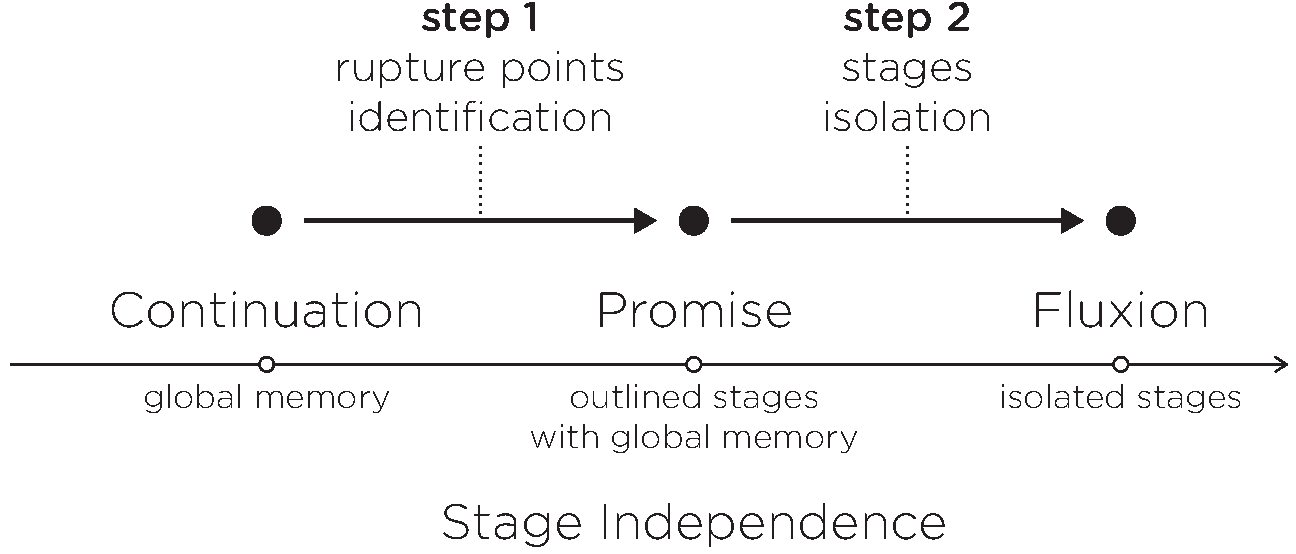
\includegraphics[width=0.7\textwidth]{../resources/roadmap.pdf}%
    \caption{Roadmap}%
    \label{fig:roadmap}%
  }%
\end{figure}

The first compiler focuses on the identification of simple chains of causality between continuations to transform these chains into Promises.
% the transformation from continuations to Promises.
% It focuses on the identification of the chains of causality in continuations.
However, promises are more expressive than the simple chaining of causal sequentiality.
% They force another control over the execution flow.
% According to the outcome of the operation, they call one function to continue the execution with the result, or another to handle errors.
% This conditional execution is indivisible from the Promise specification.
% Promises impose a convention on how to hand back the outcome of the deferred computation, while classic continuations leave this conditional execution to the developer.
Moreover, they impose a different convention than continuations on how to hand back the outcome and errors of the deferred computation.
This difference brings unnecessary complexity to the identification of chains.
To rule out this difference between continuations and Promises, before introducing the first compiler, section \ref{chapter5:due} introduces a simpler specification to Promise, called Due.

The second compiler detects all the chains of causality between continuations and encapsulate them in fluxions.
It isolates the fluxions when possible to allow the parallelism required for efficiency.
This second compilers is introduced in section \ref{chapter5:flx}.

\renewcommand{\glyph}{\iconfont{\XeTeXglyph287}}
\chapter{Implementations} \label{chapter5}
\minitoc
\eject
The transformation allowed by the equivalence from an event-driven program into a distributed network of fluxions is implemented incrementally into two compilers, as presented in figure \ref{fig:roadmap}.
Each compilers is divided into two steps, the identification of the rupture points separating the stages of the pipeline, and the isolation of these stages.
% This chapter presents the technical implementations of these two steps in the transformation from the event-driven execution model to the pipeline architecture
% , the transformation described in the previous chapter was implemented incrementally in two compilers.

\begin{figure}[h!]%
  \textfig{%
    \includegraphics[width=0.7\textwidth]{../resources/roadmap.pdf}%
    \caption{Roadmap}%
    \label{fig:roadmap}%
  }%
\end{figure}

The first compiler focuses on the identification of simple chains of causality between continuations to transform these chains into Promises.
% the transformation from continuations to Promises.
% It focuses on the identification of the chains of causality in continuations.
However, promises are more expressive than the simple chaining of causal sequentiality.
% They force another control over the execution flow.
% According to the outcome of the operation, they call one function to continue the execution with the result, or another to handle errors.
% This conditional execution is indivisible from the Promise specification.
% Promises impose a convention on how to hand back the outcome of the deferred computation, while classic continuations leave this conditional execution to the developer.
Moreover, they impose a different convention than continuations on how to hand back the outcome and errors of the deferred computation.
This difference brings unnecessary complexity to the identification of chains.
To rule out this difference between continuations and Promises, before introducing the first compiler, section \ref{chapter5:due} introduces a simpler specification to Promise, called Due.

The second compiler detects all the chains of causality between continuations and encapsulate them in fluxions.
It isolates the fluxions when possible to allow the parallelism required for efficiency.
This second compilers is introduced in section \ref{chapter5:flx}.

\input{05-implementation/Due/main}
\input{05-implementation/Flx/main}
% \input{05-implementation/Evaluation}

\renewcommand{\glyph}{\iconfont{\XeTeXglyph287}}
\chapter{Implementations} \label{chapter5}
\minitoc
\eject
The transformation allowed by the equivalence from an event-driven program into a distributed network of fluxions is implemented incrementally into two compilers, as presented in figure \ref{fig:roadmap}.
Each compilers is divided into two steps, the identification of the rupture points separating the stages of the pipeline, and the isolation of these stages.
% This chapter presents the technical implementations of these two steps in the transformation from the event-driven execution model to the pipeline architecture
% , the transformation described in the previous chapter was implemented incrementally in two compilers.

\begin{figure}[h!]%
  \textfig{%
    \includegraphics[width=0.7\textwidth]{../resources/roadmap.pdf}%
    \caption{Roadmap}%
    \label{fig:roadmap}%
  }%
\end{figure}

The first compiler focuses on the identification of simple chains of causality between continuations to transform these chains into Promises.
% the transformation from continuations to Promises.
% It focuses on the identification of the chains of causality in continuations.
However, promises are more expressive than the simple chaining of causal sequentiality.
% They force another control over the execution flow.
% According to the outcome of the operation, they call one function to continue the execution with the result, or another to handle errors.
% This conditional execution is indivisible from the Promise specification.
% Promises impose a convention on how to hand back the outcome of the deferred computation, while classic continuations leave this conditional execution to the developer.
Moreover, they impose a different convention than continuations on how to hand back the outcome and errors of the deferred computation.
This difference brings unnecessary complexity to the identification of chains.
To rule out this difference between continuations and Promises, before introducing the first compiler, section \ref{chapter5:due} introduces a simpler specification to Promise, called Due.

The second compiler detects all the chains of causality between continuations and encapsulate them in fluxions.
It isolates the fluxions when possible to allow the parallelism required for efficiency.
This second compilers is introduced in section \ref{chapter5:flx}.

\input{05-implementation/Due/main}
\input{05-implementation/Flx/main}
% \input{05-implementation/Evaluation}

% \subsection{Real test case} \label{chapter5:flx:evaluation}

The compiler is tested on a real application, gifsockets-server\ftnt{https://github.com/twolfson/gifsockets-server}.
This test proves the possibility for an application to be compiled into a network of independent parts.
It shows the current limitations of this isolation and the modifications needed on the application to circumvent them.

\begin{code}[js, caption={Simplified version of gifsockets-server},label={lst:gifsocket}]
var express = require('express'),
    app = express(),
    routes = require('gifsockets-middleware'), //@\label{lst:gifsocket:gif-mw}@
    getRawBody = require('raw-body');

function bodyParser(limit) { //@\label{lst:gifsocket:bodyParser}@
  return function saveBody(req, res, next) { //@\label{lst:gifsocket:saveBody}@
    getRawBody(req, { //@\label{lst:gifsocket:getRawBody}@
      expected: req.headers['content-length'],
      limit: limit
    }, function (err, buffer) { //@\label{lst:gifsocket:callback}@
      req.body = buffer;
      next(); //@\label{lst:gifsocket:next}@
    });
  };
}

app.post('/image/text', bodyParser(1 * 1024 * 1024), routes.writeTextToImages); //@\label{lst:gifsocket:app.post}@
app.listen(8000);
\end{code}

This application, simplified in listing \ref{lst:gifsocket}, is a real-time chat using gif-based communication channels.
It was selected from the evaluation set of the Due compiler because it is simple enough to illustrate this evaluation.
% \cite{Brodu2015}
%  from the \texttt{npm} registry because it depends on \texttt{express}, it is tested, working, and simple enough to illustrate this evaluation.
The server transforms the received text into a gif frame, and pushes it back to a never-ending gif to be displayed on the client.

On line \ref{lst:gifsocket:app.post}, the application registers two functions to process the requests received on the url \texttt{/image/text}.
The closure \texttt{saveBody}, line \ref{lst:gifsocket:saveBody}, returned by \texttt{bodyParser}, line \ref{lst:gifsocket:bodyParser}, and the method \texttt{routes.write\-Text\-To\-Images} from the external module \texttt{gifsockets-\-middleware}, line \ref{lst:gifsocket:gif-mw}.
The closure \texttt{saveBody} calls the asynchronous function \texttt{getRawBody} to get the request body.
Its callback handles the errors, and calls \texttt{next} to continue processing the request with the next function, \texttt{routes.write\-Text\-To\-Images}.

\subsubsection{Compilation} \label{chapter5:flx:evaluation:compilation}

% We compile this application with the compiler
The compilation result is in listing \ref{lst:flx-gifsocket}.
The function call \texttt{app.post}, line \ref{lst:gifsocket:app.post}, is a rupture point.
However, its callbacks, \texttt{bodyParser} and \texttt{routes.write\-Text\-To\-Images} are not declared \textit{in situ}.
They are evaluated as functions only at runtime.
As precised previously, the compiler discards these callbacks to avoid altering the semantic. % by moving or modifying their definition.
% For this reason, the compiler ignores this rupture point, to avoid interfering with the evaluation.

\begin{code}[flx, caption={Compilation result of gifsockets-server},label={lst:flx-gifsocket}]
flx main & express {req}
>> anonymous_1000 [req, next]
  var express = require('express'),
      app = express(),
      routes = require('gifsockets-middleware'), //@\label{lst:flx-gifsocket:gif-mw}@
      getRawBody = require('raw-body');

  function bodyParser(limit) { //@\label{lst:flx-gifsocket:bodyParser}@
    return function saveBody(req, res, next) { //@\label{lst:flx-gifsocket:saveBody}@
      getRawBody(req, { //@\label{lst:flx-gifsocket:getRawBody}@
        expected: req.headers['content-length'], //@\label{lst:flx-gifsocket:req.headers}@
        limit: limit
      }, >> anonymous_1000 [req, next]);
    };
  }

  app.post('/image/text', bodyParser(1 * 1024 * 1024), routes.writeTextToImages); //@\label{lst:flx-gifsocket:app.post}@
  app.listen(8000);

flx anonymous_1000
-> null
  function (err, buffer) { //@\label{lst:flx-gifsocket:callback}@
    req.body = buffer; //@\label{lst:flx-gifsocket:buffer}@
    next(); //@\label{lst:flx-gifsocket:next}@
  }
\end{code}

The compiler detects a rupture point : the function \texttt{get\-Raw\-Body} and its anonymous callback, line \ref{lst:gifsocket:callback}.
It encapsulates this callback in a fluxion named \texttt{anony\-mous\_\-1000}.
The callback is replaced with a stream placeholder to send the message stream to this downstream fluxion.
The variables \texttt{req} and \texttt{next} are appended to this message stream, to propagate their value from the \texttt{main} fluxion to the \texttt{anony\-mous\_\-1000} fluxion.

When \texttt{anony\-mous\_\-1000} is not isolated from the \texttt{main} fluxion, as if they belong to the same group, the compilation result works as expected.
The variables used in the fluxion, \texttt{req} and \texttt{next}, are still shared between the two fluxions.
In this situation fluxions are quite similar to Dues regarding memory shareing.
Our goal is to isolate the two fluxions, to be able to safely parallelize their executions.

\subsubsection{Isolation} \label{chapter5:flx:evaluation:isolation}

In listing \ref{lst:flx-gifsocket}, the fluxion \texttt{anony\-mous\_\-1000} modifies the object \texttt{req}, line \ref{lst:flx-gifsocket:buffer}, to store the text of the received request, and it calls \texttt{next} to continue the execution, line \ref{lst:flx-gifsocket:next}.
\texttt{req} is an alias to a memory location used in multiple palces in code.
Therefore, these operations produce side-effects that should propagate in the whole application, but the isolation prevents this propagation.
Isolating the fluxion \texttt{anony\-mous\_\-1000} produces runtime exceptions.
The next paragraph details how this situation is handled to allow the application to be parallelized.

\paragraph{Variable \texttt{req}}

The variable \texttt{req} is read in fluxion \texttt{main}, lines \ref{lst:flx-gifsocket:getRawBody} and \ref{lst:flx-gifsocket:req.headers}.
Then its property \texttt{body} is associated to \texttt{buffer} in fluxion \texttt{anony\-mous\_\-1000}, line \ref{lst:flx-gifsocket:buffer}.
The compiler is unable to identify the aliases of this variable. % further usages.
However, the side effect resulting from this association impacts a variable in the scope of the next callback, \texttt{routes.write\-Text\-To\-Images}.
In this test case, the application is modified manually to explicitly propagate this side-effect to the next callback through the function \texttt{next}.
The modifications of this function are explained further in the next paragraph.

\paragraph{Closure \texttt{next}}

The function \texttt{next} is a closure provided by the \texttt{express} \texttt{Router} to continue the execution with the next function to handle the client request.
Because it indirectly relies on the variable \texttt{req}, it is impossible to isolate its execution with the \texttt{anony\-mous\_\-1000} fluxion.
Instead, we modify \texttt{express}, so as to be compatible with the fluxional execution model.
We explain the modifications below.

\begin{code}[flx, caption={Simplified modification on the compiled result},label={lst:mflx-gifsocket}]
flx anonymous_1000
-> express_dispatcher
  function (err, buffer) { //@\label{lst:mflx-gifsocket:callback}@
    req.body = buffer; //@\label{lst:mflx-gifsocket:buffer}@
    next_placeholder(req, -> express_dispatcher); //@\label{lst:mflx-gifsocket:next-placeholder}@
  }

flx express_dispatcher & express {req} //@\label{lst:mflx-gifsocket:express-dispatcher}@
-> null
  function (modified_req) {
    merge(req, modified_req);
    next(); //@\label{lst:mflx-gifsocket:next}@
  }
\end{code}

In listing \ref{lst:gifsocket}, the function \texttt{next} is a continuation allowing the anonymous callback, line \ref{lst:gifsocket:callback}, to call the next function to handle the request.
To isolate the anonymous callback into \texttt{anonymous\_\-1000}, \texttt{next} is replaced by a rupture point.
This replacement is illustrated in listing \ref{lst:mflx-gifsocket}.
The \texttt{express} \texttt{Router} registers a fluxion named \texttt{express\_\-dispatcher}, line \ref{lst:mflx-gifsocket:express-dispatcher}, to continue the execution after the fluxion \texttt{anony\-mous\_\-1000}.
This fluxion is in the same group \texttt{express} as the \texttt{main} fluxion, hence it has access to the original variable \texttt{req}, and to the original function \texttt{next}.
The call to the original \texttt{next} function is replaced by a placeholder to push the stream to the fluxion \texttt{express\_\-dispatcher}, line \ref{lst:mflx-gifsocket:next-placeholder}.
The fluxion \texttt{express\_\-dispatcher} receives the stream from the upstream fluxion \texttt{anony\-mous\_\-1000}, merges back the modification in the variable \texttt{req} to propagate the side effects, and finally calls the original function \texttt{next} to continue the execution, line \ref{lst:mflx-gifsocket:next}.

After the modifications detailed above, the server works as expected.
The isolated fluxion correctly receives, and returns its serialized messages.
The client successfully receives a gif frame containing the text.



\subsection{Limitations}

The static analysis used for this compiler presents some limitations.
It is unable to analyze code with dynamic behaviors.
Higher-order programming leads to more productivity partly beacuse it rely on such dynamic behavior to extend expressivity.
Precisely, it allows more levels of indirections.

\subsubsection{Levels of Indirections}

The indirection is an abstraction between the value, and its manipulation.
In listing \ref{lst:indirection}, the variables \texttt{a} and \texttt{b} point both to the same memory object.
The function \texttt{fn} introduces a level of indirection between the real object \texttt{a} and its manipulation handle, \texttt{b};
% Actually, the variable \texttt{a} already introduces a level of indirection between the real object and the handle \texttt{a}.

\begin{code}[js,
  caption={One level of Indirection},
  label={lst:indirection}]
var a = {
      // an object;
    };

fn(b) {
  // modify b;
}

fn(a);
\end{code}

\subsubsection{Uncertainties}

The indirection is trivial to resolve in listing \ref{lst:indirection}.
It only needs to have access to the definition of \texttt{a} and of \texttt{fn}.
%A very simple static analysis could resolve it.
However, in listing \ref{lst:indirections}, the array \texttt{handlers} introduces a new level of indirection.
The static analysis now needs to have access to the definition of \texttt{i} and of the \texttt{handlers}.
If this definition is provided by an external input, it is not available statically, hence, it adds an uncertainty during the analysis. 

\begin{code}[js,
  caption={Two levels of indirection},
  label={lst:indirections}]
var a = {
      // an object;
    },
    handlers = [
      // definition of fn handlers;
    ],
    i = ?;

handlers[i](a);
handlers[i+1](a);
\end{code}

These examples are extremely simplified.
A real application contains enough indirections for the static analysis to be overwhelmed by uncertainties, and to be unable to resolve the variables.
If a variable is left unresolved, it is impossible to assure its scope and its aliases.
Therefore, the compiler is unable to isolate it into a fluxion, or to distribute its modification by messages.

Moreover, it leads the compiler to ignore the rupture points not defined \textit{in situ}, because their modifications could impact the semantic.
The reason for this precaution, is that the compiler is unable to assure where the function is used, and the scope of its variables.
Therefore, it is unable to assure that the modification will conserve the semantic.

\subsubsection{Dynamic Resolution}

In a web application, this variable \texttt{i} might be part of the user request, which is available only at runtime.
It eventually introduces an uncertainty.

This dynamic resolution of variables is precisely what increase expressiveness.
Trying to resolve them statically is equivalent to restrict expressiveness.
No static analysis can overstep these limitations.
Only a dynamic analysis could analysis the resolved indirections during run time to overstep these limitations correctly.




\renewcommand{\glyph}{\iconfont{\XeTeXglyph287}}
\chapter{Implementations} \label{chapter5}
\minitoc
\eject
The transformation allowed by the equivalence from an event-driven program into a distributed network of fluxions is implemented incrementally into two compilers, as presented in figure \ref{fig:roadmap}.
Each compilers is divided into two steps, the identification of the rupture points separating the stages of the pipeline, and the isolation of these stages.
% This chapter presents the technical implementations of these two steps in the transformation from the event-driven execution model to the pipeline architecture
% , the transformation described in the previous chapter was implemented incrementally in two compilers.

\begin{figure}[h!]%
  \textfig{%
    \includegraphics[width=0.7\textwidth]{../resources/roadmap.pdf}%
    \caption{Roadmap}%
    \label{fig:roadmap}%
  }%
\end{figure}

The first compiler focuses on the identification of simple chains of causality between continuations to transform these chains into Promises.
% the transformation from continuations to Promises.
% It focuses on the identification of the chains of causality in continuations.
However, promises are more expressive than the simple chaining of causal sequentiality.
% They force another control over the execution flow.
% According to the outcome of the operation, they call one function to continue the execution with the result, or another to handle errors.
% This conditional execution is indivisible from the Promise specification.
% Promises impose a convention on how to hand back the outcome of the deferred computation, while classic continuations leave this conditional execution to the developer.
Moreover, they impose a different convention than continuations on how to hand back the outcome and errors of the deferred computation.
This difference brings unnecessary complexity to the identification of chains.
To rule out this difference between continuations and Promises, before introducing the first compiler, section \ref{chapter5:due} introduces a simpler specification to Promise, called Due.

The second compiler detects all the chains of causality between continuations and encapsulate them in fluxions.
It isolates the fluxions when possible to allow the parallelism required for efficiency.
This second compilers is introduced in section \ref{chapter5:flx}.

\renewcommand{\glyph}{\iconfont{\XeTeXglyph287}}
\chapter{Implementations} \label{chapter5}
\minitoc
\eject
The transformation allowed by the equivalence from an event-driven program into a distributed network of fluxions is implemented incrementally into two compilers, as presented in figure \ref{fig:roadmap}.
Each compilers is divided into two steps, the identification of the rupture points separating the stages of the pipeline, and the isolation of these stages.
% This chapter presents the technical implementations of these two steps in the transformation from the event-driven execution model to the pipeline architecture
% , the transformation described in the previous chapter was implemented incrementally in two compilers.

\begin{figure}[h!]%
  \textfig{%
    \includegraphics[width=0.7\textwidth]{../resources/roadmap.pdf}%
    \caption{Roadmap}%
    \label{fig:roadmap}%
  }%
\end{figure}

The first compiler focuses on the identification of simple chains of causality between continuations to transform these chains into Promises.
% the transformation from continuations to Promises.
% It focuses on the identification of the chains of causality in continuations.
However, promises are more expressive than the simple chaining of causal sequentiality.
% They force another control over the execution flow.
% According to the outcome of the operation, they call one function to continue the execution with the result, or another to handle errors.
% This conditional execution is indivisible from the Promise specification.
% Promises impose a convention on how to hand back the outcome of the deferred computation, while classic continuations leave this conditional execution to the developer.
Moreover, they impose a different convention than continuations on how to hand back the outcome and errors of the deferred computation.
This difference brings unnecessary complexity to the identification of chains.
To rule out this difference between continuations and Promises, before introducing the first compiler, section \ref{chapter5:due} introduces a simpler specification to Promise, called Due.

The second compiler detects all the chains of causality between continuations and encapsulate them in fluxions.
It isolates the fluxions when possible to allow the parallelism required for efficiency.
This second compilers is introduced in section \ref{chapter5:flx}.

\input{05-implementation/Due/main}
\input{05-implementation/Flx/main}
% \input{05-implementation/Evaluation}

\renewcommand{\glyph}{\iconfont{\XeTeXglyph287}}
\chapter{Implementations} \label{chapter5}
\minitoc
\eject
The transformation allowed by the equivalence from an event-driven program into a distributed network of fluxions is implemented incrementally into two compilers, as presented in figure \ref{fig:roadmap}.
Each compilers is divided into two steps, the identification of the rupture points separating the stages of the pipeline, and the isolation of these stages.
% This chapter presents the technical implementations of these two steps in the transformation from the event-driven execution model to the pipeline architecture
% , the transformation described in the previous chapter was implemented incrementally in two compilers.

\begin{figure}[h!]%
  \textfig{%
    \includegraphics[width=0.7\textwidth]{../resources/roadmap.pdf}%
    \caption{Roadmap}%
    \label{fig:roadmap}%
  }%
\end{figure}

The first compiler focuses on the identification of simple chains of causality between continuations to transform these chains into Promises.
% the transformation from continuations to Promises.
% It focuses on the identification of the chains of causality in continuations.
However, promises are more expressive than the simple chaining of causal sequentiality.
% They force another control over the execution flow.
% According to the outcome of the operation, they call one function to continue the execution with the result, or another to handle errors.
% This conditional execution is indivisible from the Promise specification.
% Promises impose a convention on how to hand back the outcome of the deferred computation, while classic continuations leave this conditional execution to the developer.
Moreover, they impose a different convention than continuations on how to hand back the outcome and errors of the deferred computation.
This difference brings unnecessary complexity to the identification of chains.
To rule out this difference between continuations and Promises, before introducing the first compiler, section \ref{chapter5:due} introduces a simpler specification to Promise, called Due.

The second compiler detects all the chains of causality between continuations and encapsulate them in fluxions.
It isolates the fluxions when possible to allow the parallelism required for efficiency.
This second compilers is introduced in section \ref{chapter5:flx}.

\input{05-implementation/Due/main}
\input{05-implementation/Flx/main}
% \input{05-implementation/Evaluation}

% \subsection{Real test case} \label{chapter5:flx:evaluation}

The compiler is tested on a real application, gifsockets-server\ftnt{https://github.com/twolfson/gifsockets-server}.
This test proves the possibility for an application to be compiled into a network of independent parts.
It shows the current limitations of this isolation and the modifications needed on the application to circumvent them.

\begin{code}[js, caption={Simplified version of gifsockets-server},label={lst:gifsocket}]
var express = require('express'),
    app = express(),
    routes = require('gifsockets-middleware'), //@\label{lst:gifsocket:gif-mw}@
    getRawBody = require('raw-body');

function bodyParser(limit) { //@\label{lst:gifsocket:bodyParser}@
  return function saveBody(req, res, next) { //@\label{lst:gifsocket:saveBody}@
    getRawBody(req, { //@\label{lst:gifsocket:getRawBody}@
      expected: req.headers['content-length'],
      limit: limit
    }, function (err, buffer) { //@\label{lst:gifsocket:callback}@
      req.body = buffer;
      next(); //@\label{lst:gifsocket:next}@
    });
  };
}

app.post('/image/text', bodyParser(1 * 1024 * 1024), routes.writeTextToImages); //@\label{lst:gifsocket:app.post}@
app.listen(8000);
\end{code}

This application, simplified in listing \ref{lst:gifsocket}, is a real-time chat using gif-based communication channels.
It was selected from the evaluation set of the Due compiler because it is simple enough to illustrate this evaluation.
% \cite{Brodu2015}
%  from the \texttt{npm} registry because it depends on \texttt{express}, it is tested, working, and simple enough to illustrate this evaluation.
The server transforms the received text into a gif frame, and pushes it back to a never-ending gif to be displayed on the client.

On line \ref{lst:gifsocket:app.post}, the application registers two functions to process the requests received on the url \texttt{/image/text}.
The closure \texttt{saveBody}, line \ref{lst:gifsocket:saveBody}, returned by \texttt{bodyParser}, line \ref{lst:gifsocket:bodyParser}, and the method \texttt{routes.write\-Text\-To\-Images} from the external module \texttt{gifsockets-\-middleware}, line \ref{lst:gifsocket:gif-mw}.
The closure \texttt{saveBody} calls the asynchronous function \texttt{getRawBody} to get the request body.
Its callback handles the errors, and calls \texttt{next} to continue processing the request with the next function, \texttt{routes.write\-Text\-To\-Images}.

\subsubsection{Compilation} \label{chapter5:flx:evaluation:compilation}

% We compile this application with the compiler
The compilation result is in listing \ref{lst:flx-gifsocket}.
The function call \texttt{app.post}, line \ref{lst:gifsocket:app.post}, is a rupture point.
However, its callbacks, \texttt{bodyParser} and \texttt{routes.write\-Text\-To\-Images} are not declared \textit{in situ}.
They are evaluated as functions only at runtime.
As precised previously, the compiler discards these callbacks to avoid altering the semantic. % by moving or modifying their definition.
% For this reason, the compiler ignores this rupture point, to avoid interfering with the evaluation.

\begin{code}[flx, caption={Compilation result of gifsockets-server},label={lst:flx-gifsocket}]
flx main & express {req}
>> anonymous_1000 [req, next]
  var express = require('express'),
      app = express(),
      routes = require('gifsockets-middleware'), //@\label{lst:flx-gifsocket:gif-mw}@
      getRawBody = require('raw-body');

  function bodyParser(limit) { //@\label{lst:flx-gifsocket:bodyParser}@
    return function saveBody(req, res, next) { //@\label{lst:flx-gifsocket:saveBody}@
      getRawBody(req, { //@\label{lst:flx-gifsocket:getRawBody}@
        expected: req.headers['content-length'], //@\label{lst:flx-gifsocket:req.headers}@
        limit: limit
      }, >> anonymous_1000 [req, next]);
    };
  }

  app.post('/image/text', bodyParser(1 * 1024 * 1024), routes.writeTextToImages); //@\label{lst:flx-gifsocket:app.post}@
  app.listen(8000);

flx anonymous_1000
-> null
  function (err, buffer) { //@\label{lst:flx-gifsocket:callback}@
    req.body = buffer; //@\label{lst:flx-gifsocket:buffer}@
    next(); //@\label{lst:flx-gifsocket:next}@
  }
\end{code}

The compiler detects a rupture point : the function \texttt{get\-Raw\-Body} and its anonymous callback, line \ref{lst:gifsocket:callback}.
It encapsulates this callback in a fluxion named \texttt{anony\-mous\_\-1000}.
The callback is replaced with a stream placeholder to send the message stream to this downstream fluxion.
The variables \texttt{req} and \texttt{next} are appended to this message stream, to propagate their value from the \texttt{main} fluxion to the \texttt{anony\-mous\_\-1000} fluxion.

When \texttt{anony\-mous\_\-1000} is not isolated from the \texttt{main} fluxion, as if they belong to the same group, the compilation result works as expected.
The variables used in the fluxion, \texttt{req} and \texttt{next}, are still shared between the two fluxions.
In this situation fluxions are quite similar to Dues regarding memory shareing.
Our goal is to isolate the two fluxions, to be able to safely parallelize their executions.

\subsubsection{Isolation} \label{chapter5:flx:evaluation:isolation}

In listing \ref{lst:flx-gifsocket}, the fluxion \texttt{anony\-mous\_\-1000} modifies the object \texttt{req}, line \ref{lst:flx-gifsocket:buffer}, to store the text of the received request, and it calls \texttt{next} to continue the execution, line \ref{lst:flx-gifsocket:next}.
\texttt{req} is an alias to a memory location used in multiple palces in code.
Therefore, these operations produce side-effects that should propagate in the whole application, but the isolation prevents this propagation.
Isolating the fluxion \texttt{anony\-mous\_\-1000} produces runtime exceptions.
The next paragraph details how this situation is handled to allow the application to be parallelized.

\paragraph{Variable \texttt{req}}

The variable \texttt{req} is read in fluxion \texttt{main}, lines \ref{lst:flx-gifsocket:getRawBody} and \ref{lst:flx-gifsocket:req.headers}.
Then its property \texttt{body} is associated to \texttt{buffer} in fluxion \texttt{anony\-mous\_\-1000}, line \ref{lst:flx-gifsocket:buffer}.
The compiler is unable to identify the aliases of this variable. % further usages.
However, the side effect resulting from this association impacts a variable in the scope of the next callback, \texttt{routes.write\-Text\-To\-Images}.
In this test case, the application is modified manually to explicitly propagate this side-effect to the next callback through the function \texttt{next}.
The modifications of this function are explained further in the next paragraph.

\paragraph{Closure \texttt{next}}

The function \texttt{next} is a closure provided by the \texttt{express} \texttt{Router} to continue the execution with the next function to handle the client request.
Because it indirectly relies on the variable \texttt{req}, it is impossible to isolate its execution with the \texttt{anony\-mous\_\-1000} fluxion.
Instead, we modify \texttt{express}, so as to be compatible with the fluxional execution model.
We explain the modifications below.

\begin{code}[flx, caption={Simplified modification on the compiled result},label={lst:mflx-gifsocket}]
flx anonymous_1000
-> express_dispatcher
  function (err, buffer) { //@\label{lst:mflx-gifsocket:callback}@
    req.body = buffer; //@\label{lst:mflx-gifsocket:buffer}@
    next_placeholder(req, -> express_dispatcher); //@\label{lst:mflx-gifsocket:next-placeholder}@
  }

flx express_dispatcher & express {req} //@\label{lst:mflx-gifsocket:express-dispatcher}@
-> null
  function (modified_req) {
    merge(req, modified_req);
    next(); //@\label{lst:mflx-gifsocket:next}@
  }
\end{code}

In listing \ref{lst:gifsocket}, the function \texttt{next} is a continuation allowing the anonymous callback, line \ref{lst:gifsocket:callback}, to call the next function to handle the request.
To isolate the anonymous callback into \texttt{anonymous\_\-1000}, \texttt{next} is replaced by a rupture point.
This replacement is illustrated in listing \ref{lst:mflx-gifsocket}.
The \texttt{express} \texttt{Router} registers a fluxion named \texttt{express\_\-dispatcher}, line \ref{lst:mflx-gifsocket:express-dispatcher}, to continue the execution after the fluxion \texttt{anony\-mous\_\-1000}.
This fluxion is in the same group \texttt{express} as the \texttt{main} fluxion, hence it has access to the original variable \texttt{req}, and to the original function \texttt{next}.
The call to the original \texttt{next} function is replaced by a placeholder to push the stream to the fluxion \texttt{express\_\-dispatcher}, line \ref{lst:mflx-gifsocket:next-placeholder}.
The fluxion \texttt{express\_\-dispatcher} receives the stream from the upstream fluxion \texttt{anony\-mous\_\-1000}, merges back the modification in the variable \texttt{req} to propagate the side effects, and finally calls the original function \texttt{next} to continue the execution, line \ref{lst:mflx-gifsocket:next}.

After the modifications detailed above, the server works as expected.
The isolated fluxion correctly receives, and returns its serialized messages.
The client successfully receives a gif frame containing the text.



\subsection{Limitations}

The static analysis used for this compiler presents some limitations.
It is unable to analyze code with dynamic behaviors.
Higher-order programming leads to more productivity partly beacuse it rely on such dynamic behavior to extend expressivity.
Precisely, it allows more levels of indirections.

\subsubsection{Levels of Indirections}

The indirection is an abstraction between the value, and its manipulation.
In listing \ref{lst:indirection}, the variables \texttt{a} and \texttt{b} point both to the same memory object.
The function \texttt{fn} introduces a level of indirection between the real object \texttt{a} and its manipulation handle, \texttt{b};
% Actually, the variable \texttt{a} already introduces a level of indirection between the real object and the handle \texttt{a}.

\begin{code}[js,
  caption={One level of Indirection},
  label={lst:indirection}]
var a = {
      // an object;
    };

fn(b) {
  // modify b;
}

fn(a);
\end{code}

\subsubsection{Uncertainties}

The indirection is trivial to resolve in listing \ref{lst:indirection}.
It only needs to have access to the definition of \texttt{a} and of \texttt{fn}.
%A very simple static analysis could resolve it.
However, in listing \ref{lst:indirections}, the array \texttt{handlers} introduces a new level of indirection.
The static analysis now needs to have access to the definition of \texttt{i} and of the \texttt{handlers}.
If this definition is provided by an external input, it is not available statically, hence, it adds an uncertainty during the analysis. 

\begin{code}[js,
  caption={Two levels of indirection},
  label={lst:indirections}]
var a = {
      // an object;
    },
    handlers = [
      // definition of fn handlers;
    ],
    i = ?;

handlers[i](a);
handlers[i+1](a);
\end{code}

These examples are extremely simplified.
A real application contains enough indirections for the static analysis to be overwhelmed by uncertainties, and to be unable to resolve the variables.
If a variable is left unresolved, it is impossible to assure its scope and its aliases.
Therefore, the compiler is unable to isolate it into a fluxion, or to distribute its modification by messages.

Moreover, it leads the compiler to ignore the rupture points not defined \textit{in situ}, because their modifications could impact the semantic.
The reason for this precaution, is that the compiler is unable to assure where the function is used, and the scope of its variables.
Therefore, it is unable to assure that the modification will conserve the semantic.

\subsubsection{Dynamic Resolution}

In a web application, this variable \texttt{i} might be part of the user request, which is available only at runtime.
It eventually introduces an uncertainty.

This dynamic resolution of variables is precisely what increase expressiveness.
Trying to resolve them statically is equivalent to restrict expressiveness.
No static analysis can overstep these limitations.
Only a dynamic analysis could analysis the resolved indirections during run time to overstep these limitations correctly.




% \subsection{Real test case} \label{chapter5:flx:evaluation}

The compiler is tested on a real application, gifsockets-server\ftnt{https://github.com/twolfson/gifsockets-server}.
This test proves the possibility for an application to be compiled into a network of independent parts.
It shows the current limitations of this isolation and the modifications needed on the application to circumvent them.

\begin{code}[js, caption={Simplified version of gifsockets-server},label={lst:gifsocket}]
var express = require('express'),
    app = express(),
    routes = require('gifsockets-middleware'), //@\label{lst:gifsocket:gif-mw}@
    getRawBody = require('raw-body');

function bodyParser(limit) { //@\label{lst:gifsocket:bodyParser}@
  return function saveBody(req, res, next) { //@\label{lst:gifsocket:saveBody}@
    getRawBody(req, { //@\label{lst:gifsocket:getRawBody}@
      expected: req.headers['content-length'],
      limit: limit
    }, function (err, buffer) { //@\label{lst:gifsocket:callback}@
      req.body = buffer;
      next(); //@\label{lst:gifsocket:next}@
    });
  };
}

app.post('/image/text', bodyParser(1 * 1024 * 1024), routes.writeTextToImages); //@\label{lst:gifsocket:app.post}@
app.listen(8000);
\end{code}

This application, simplified in listing \ref{lst:gifsocket}, is a real-time chat using gif-based communication channels.
It was selected from the evaluation set of the Due compiler because it is simple enough to illustrate this evaluation.
% \cite{Brodu2015}
%  from the \texttt{npm} registry because it depends on \texttt{express}, it is tested, working, and simple enough to illustrate this evaluation.
The server transforms the received text into a gif frame, and pushes it back to a never-ending gif to be displayed on the client.

On line \ref{lst:gifsocket:app.post}, the application registers two functions to process the requests received on the url \texttt{/image/text}.
The closure \texttt{saveBody}, line \ref{lst:gifsocket:saveBody}, returned by \texttt{bodyParser}, line \ref{lst:gifsocket:bodyParser}, and the method \texttt{routes.write\-Text\-To\-Images} from the external module \texttt{gifsockets-\-middleware}, line \ref{lst:gifsocket:gif-mw}.
The closure \texttt{saveBody} calls the asynchronous function \texttt{getRawBody} to get the request body.
Its callback handles the errors, and calls \texttt{next} to continue processing the request with the next function, \texttt{routes.write\-Text\-To\-Images}.

\subsubsection{Compilation} \label{chapter5:flx:evaluation:compilation}

% We compile this application with the compiler
The compilation result is in listing \ref{lst:flx-gifsocket}.
The function call \texttt{app.post}, line \ref{lst:gifsocket:app.post}, is a rupture point.
However, its callbacks, \texttt{bodyParser} and \texttt{routes.write\-Text\-To\-Images} are not declared \textit{in situ}.
They are evaluated as functions only at runtime.
As precised previously, the compiler discards these callbacks to avoid altering the semantic. % by moving or modifying their definition.
% For this reason, the compiler ignores this rupture point, to avoid interfering with the evaluation.

\begin{code}[flx, caption={Compilation result of gifsockets-server},label={lst:flx-gifsocket}]
flx main & express {req}
>> anonymous_1000 [req, next]
  var express = require('express'),
      app = express(),
      routes = require('gifsockets-middleware'), //@\label{lst:flx-gifsocket:gif-mw}@
      getRawBody = require('raw-body');

  function bodyParser(limit) { //@\label{lst:flx-gifsocket:bodyParser}@
    return function saveBody(req, res, next) { //@\label{lst:flx-gifsocket:saveBody}@
      getRawBody(req, { //@\label{lst:flx-gifsocket:getRawBody}@
        expected: req.headers['content-length'], //@\label{lst:flx-gifsocket:req.headers}@
        limit: limit
      }, >> anonymous_1000 [req, next]);
    };
  }

  app.post('/image/text', bodyParser(1 * 1024 * 1024), routes.writeTextToImages); //@\label{lst:flx-gifsocket:app.post}@
  app.listen(8000);

flx anonymous_1000
-> null
  function (err, buffer) { //@\label{lst:flx-gifsocket:callback}@
    req.body = buffer; //@\label{lst:flx-gifsocket:buffer}@
    next(); //@\label{lst:flx-gifsocket:next}@
  }
\end{code}

The compiler detects a rupture point : the function \texttt{get\-Raw\-Body} and its anonymous callback, line \ref{lst:gifsocket:callback}.
It encapsulates this callback in a fluxion named \texttt{anony\-mous\_\-1000}.
The callback is replaced with a stream placeholder to send the message stream to this downstream fluxion.
The variables \texttt{req} and \texttt{next} are appended to this message stream, to propagate their value from the \texttt{main} fluxion to the \texttt{anony\-mous\_\-1000} fluxion.

When \texttt{anony\-mous\_\-1000} is not isolated from the \texttt{main} fluxion, as if they belong to the same group, the compilation result works as expected.
The variables used in the fluxion, \texttt{req} and \texttt{next}, are still shared between the two fluxions.
In this situation fluxions are quite similar to Dues regarding memory shareing.
Our goal is to isolate the two fluxions, to be able to safely parallelize their executions.

\subsubsection{Isolation} \label{chapter5:flx:evaluation:isolation}

In listing \ref{lst:flx-gifsocket}, the fluxion \texttt{anony\-mous\_\-1000} modifies the object \texttt{req}, line \ref{lst:flx-gifsocket:buffer}, to store the text of the received request, and it calls \texttt{next} to continue the execution, line \ref{lst:flx-gifsocket:next}.
\texttt{req} is an alias to a memory location used in multiple palces in code.
Therefore, these operations produce side-effects that should propagate in the whole application, but the isolation prevents this propagation.
Isolating the fluxion \texttt{anony\-mous\_\-1000} produces runtime exceptions.
The next paragraph details how this situation is handled to allow the application to be parallelized.

\paragraph{Variable \texttt{req}}

The variable \texttt{req} is read in fluxion \texttt{main}, lines \ref{lst:flx-gifsocket:getRawBody} and \ref{lst:flx-gifsocket:req.headers}.
Then its property \texttt{body} is associated to \texttt{buffer} in fluxion \texttt{anony\-mous\_\-1000}, line \ref{lst:flx-gifsocket:buffer}.
The compiler is unable to identify the aliases of this variable. % further usages.
However, the side effect resulting from this association impacts a variable in the scope of the next callback, \texttt{routes.write\-Text\-To\-Images}.
In this test case, the application is modified manually to explicitly propagate this side-effect to the next callback through the function \texttt{next}.
The modifications of this function are explained further in the next paragraph.

\paragraph{Closure \texttt{next}}

The function \texttt{next} is a closure provided by the \texttt{express} \texttt{Router} to continue the execution with the next function to handle the client request.
Because it indirectly relies on the variable \texttt{req}, it is impossible to isolate its execution with the \texttt{anony\-mous\_\-1000} fluxion.
Instead, we modify \texttt{express}, so as to be compatible with the fluxional execution model.
We explain the modifications below.

\begin{code}[flx, caption={Simplified modification on the compiled result},label={lst:mflx-gifsocket}]
flx anonymous_1000
-> express_dispatcher
  function (err, buffer) { //@\label{lst:mflx-gifsocket:callback}@
    req.body = buffer; //@\label{lst:mflx-gifsocket:buffer}@
    next_placeholder(req, -> express_dispatcher); //@\label{lst:mflx-gifsocket:next-placeholder}@
  }

flx express_dispatcher & express {req} //@\label{lst:mflx-gifsocket:express-dispatcher}@
-> null
  function (modified_req) {
    merge(req, modified_req);
    next(); //@\label{lst:mflx-gifsocket:next}@
  }
\end{code}

In listing \ref{lst:gifsocket}, the function \texttt{next} is a continuation allowing the anonymous callback, line \ref{lst:gifsocket:callback}, to call the next function to handle the request.
To isolate the anonymous callback into \texttt{anonymous\_\-1000}, \texttt{next} is replaced by a rupture point.
This replacement is illustrated in listing \ref{lst:mflx-gifsocket}.
The \texttt{express} \texttt{Router} registers a fluxion named \texttt{express\_\-dispatcher}, line \ref{lst:mflx-gifsocket:express-dispatcher}, to continue the execution after the fluxion \texttt{anony\-mous\_\-1000}.
This fluxion is in the same group \texttt{express} as the \texttt{main} fluxion, hence it has access to the original variable \texttt{req}, and to the original function \texttt{next}.
The call to the original \texttt{next} function is replaced by a placeholder to push the stream to the fluxion \texttt{express\_\-dispatcher}, line \ref{lst:mflx-gifsocket:next-placeholder}.
The fluxion \texttt{express\_\-dispatcher} receives the stream from the upstream fluxion \texttt{anony\-mous\_\-1000}, merges back the modification in the variable \texttt{req} to propagate the side effects, and finally calls the original function \texttt{next} to continue the execution, line \ref{lst:mflx-gifsocket:next}.

After the modifications detailed above, the server works as expected.
The isolated fluxion correctly receives, and returns its serialized messages.
The client successfully receives a gif frame containing the text.



\subsection{Limitations}

The static analysis used for this compiler presents some limitations.
It is unable to analyze code with dynamic behaviors.
Higher-order programming leads to more productivity partly beacuse it rely on such dynamic behavior to extend expressivity.
Precisely, it allows more levels of indirections.

\subsubsection{Levels of Indirections}

The indirection is an abstraction between the value, and its manipulation.
In listing \ref{lst:indirection}, the variables \texttt{a} and \texttt{b} point both to the same memory object.
The function \texttt{fn} introduces a level of indirection between the real object \texttt{a} and its manipulation handle, \texttt{b};
% Actually, the variable \texttt{a} already introduces a level of indirection between the real object and the handle \texttt{a}.

\begin{code}[js,
  caption={One level of Indirection},
  label={lst:indirection}]
var a = {
      // an object;
    };

fn(b) {
  // modify b;
}

fn(a);
\end{code}

\subsubsection{Uncertainties}

The indirection is trivial to resolve in listing \ref{lst:indirection}.
It only needs to have access to the definition of \texttt{a} and of \texttt{fn}.
%A very simple static analysis could resolve it.
However, in listing \ref{lst:indirections}, the array \texttt{handlers} introduces a new level of indirection.
The static analysis now needs to have access to the definition of \texttt{i} and of the \texttt{handlers}.
If this definition is provided by an external input, it is not available statically, hence, it adds an uncertainty during the analysis. 

\begin{code}[js,
  caption={Two levels of indirection},
  label={lst:indirections}]
var a = {
      // an object;
    },
    handlers = [
      // definition of fn handlers;
    ],
    i = ?;

handlers[i](a);
handlers[i+1](a);
\end{code}

These examples are extremely simplified.
A real application contains enough indirections for the static analysis to be overwhelmed by uncertainties, and to be unable to resolve the variables.
If a variable is left unresolved, it is impossible to assure its scope and its aliases.
Therefore, the compiler is unable to isolate it into a fluxion, or to distribute its modification by messages.

Moreover, it leads the compiler to ignore the rupture points not defined \textit{in situ}, because their modifications could impact the semantic.
The reason for this precaution, is that the compiler is unable to assure where the function is used, and the scope of its variables.
Therefore, it is unable to assure that the modification will conserve the semantic.

\subsubsection{Dynamic Resolution}

In a web application, this variable \texttt{i} might be part of the user request, which is available only at runtime.
It eventually introduces an uncertainty.

This dynamic resolution of variables is precisely what increase expressiveness.
Trying to resolve them statically is equivalent to restrict expressiveness.
No static analysis can overstep these limitations.
Only a dynamic analysis could analysis the resolved indirections during run time to overstep these limitations correctly.





\eject
\renewcommand{\glyph}{\linecons{\XeTeXglyph39}}
\printbibliography[]

\renewcommand{\glyph}{\iconfont{\XeTeXglyph287}}
\chapter{Implementations} \label{chapter5}
\minitoc
\eject
The transformation allowed by the equivalence from an event-driven program into a distributed network of fluxions is implemented incrementally into two compilers, as presented in figure \ref{fig:roadmap}.
Each compilers is divided into two steps, the identification of the rupture points separating the stages of the pipeline, and the isolation of these stages.
% This chapter presents the technical implementations of these two steps in the transformation from the event-driven execution model to the pipeline architecture
% , the transformation described in the previous chapter was implemented incrementally in two compilers.

\begin{figure}[h!]%
  \textfig{%
    \includegraphics[width=0.7\textwidth]{../resources/roadmap.pdf}%
    \caption{Roadmap}%
    \label{fig:roadmap}%
  }%
\end{figure}

The first compiler focuses on the identification of simple chains of causality between continuations to transform these chains into Promises.
% the transformation from continuations to Promises.
% It focuses on the identification of the chains of causality in continuations.
However, promises are more expressive than the simple chaining of causal sequentiality.
% They force another control over the execution flow.
% According to the outcome of the operation, they call one function to continue the execution with the result, or another to handle errors.
% This conditional execution is indivisible from the Promise specification.
% Promises impose a convention on how to hand back the outcome of the deferred computation, while classic continuations leave this conditional execution to the developer.
Moreover, they impose a different convention than continuations on how to hand back the outcome and errors of the deferred computation.
This difference brings unnecessary complexity to the identification of chains.
To rule out this difference between continuations and Promises, before introducing the first compiler, section \ref{chapter5:due} introduces a simpler specification to Promise, called Due.

The second compiler detects all the chains of causality between continuations and encapsulate them in fluxions.
It isolates the fluxions when possible to allow the parallelism required for efficiency.
This second compilers is introduced in section \ref{chapter5:flx}.

\renewcommand{\glyph}{\iconfont{\XeTeXglyph287}}
\chapter{Implementations} \label{chapter5}
\minitoc
\eject
The transformation allowed by the equivalence from an event-driven program into a distributed network of fluxions is implemented incrementally into two compilers, as presented in figure \ref{fig:roadmap}.
Each compilers is divided into two steps, the identification of the rupture points separating the stages of the pipeline, and the isolation of these stages.
% This chapter presents the technical implementations of these two steps in the transformation from the event-driven execution model to the pipeline architecture
% , the transformation described in the previous chapter was implemented incrementally in two compilers.

\begin{figure}[h!]%
  \textfig{%
    \includegraphics[width=0.7\textwidth]{../resources/roadmap.pdf}%
    \caption{Roadmap}%
    \label{fig:roadmap}%
  }%
\end{figure}

The first compiler focuses on the identification of simple chains of causality between continuations to transform these chains into Promises.
% the transformation from continuations to Promises.
% It focuses on the identification of the chains of causality in continuations.
However, promises are more expressive than the simple chaining of causal sequentiality.
% They force another control over the execution flow.
% According to the outcome of the operation, they call one function to continue the execution with the result, or another to handle errors.
% This conditional execution is indivisible from the Promise specification.
% Promises impose a convention on how to hand back the outcome of the deferred computation, while classic continuations leave this conditional execution to the developer.
Moreover, they impose a different convention than continuations on how to hand back the outcome and errors of the deferred computation.
This difference brings unnecessary complexity to the identification of chains.
To rule out this difference between continuations and Promises, before introducing the first compiler, section \ref{chapter5:due} introduces a simpler specification to Promise, called Due.

The second compiler detects all the chains of causality between continuations and encapsulate them in fluxions.
It isolates the fluxions when possible to allow the parallelism required for efficiency.
This second compilers is introduced in section \ref{chapter5:flx}.

\renewcommand{\glyph}{\iconfont{\XeTeXglyph287}}
\chapter{Implementations} \label{chapter5}
\minitoc
\eject
The transformation allowed by the equivalence from an event-driven program into a distributed network of fluxions is implemented incrementally into two compilers, as presented in figure \ref{fig:roadmap}.
Each compilers is divided into two steps, the identification of the rupture points separating the stages of the pipeline, and the isolation of these stages.
% This chapter presents the technical implementations of these two steps in the transformation from the event-driven execution model to the pipeline architecture
% , the transformation described in the previous chapter was implemented incrementally in two compilers.

\begin{figure}[h!]%
  \textfig{%
    \includegraphics[width=0.7\textwidth]{../resources/roadmap.pdf}%
    \caption{Roadmap}%
    \label{fig:roadmap}%
  }%
\end{figure}

The first compiler focuses on the identification of simple chains of causality between continuations to transform these chains into Promises.
% the transformation from continuations to Promises.
% It focuses on the identification of the chains of causality in continuations.
However, promises are more expressive than the simple chaining of causal sequentiality.
% They force another control over the execution flow.
% According to the outcome of the operation, they call one function to continue the execution with the result, or another to handle errors.
% This conditional execution is indivisible from the Promise specification.
% Promises impose a convention on how to hand back the outcome of the deferred computation, while classic continuations leave this conditional execution to the developer.
Moreover, they impose a different convention than continuations on how to hand back the outcome and errors of the deferred computation.
This difference brings unnecessary complexity to the identification of chains.
To rule out this difference between continuations and Promises, before introducing the first compiler, section \ref{chapter5:due} introduces a simpler specification to Promise, called Due.

The second compiler detects all the chains of causality between continuations and encapsulate them in fluxions.
It isolates the fluxions when possible to allow the parallelism required for efficiency.
This second compilers is introduced in section \ref{chapter5:flx}.

\input{05-implementation/Due/main}
\input{05-implementation/Flx/main}
% \input{05-implementation/Evaluation}

\renewcommand{\glyph}{\iconfont{\XeTeXglyph287}}
\chapter{Implementations} \label{chapter5}
\minitoc
\eject
The transformation allowed by the equivalence from an event-driven program into a distributed network of fluxions is implemented incrementally into two compilers, as presented in figure \ref{fig:roadmap}.
Each compilers is divided into two steps, the identification of the rupture points separating the stages of the pipeline, and the isolation of these stages.
% This chapter presents the technical implementations of these two steps in the transformation from the event-driven execution model to the pipeline architecture
% , the transformation described in the previous chapter was implemented incrementally in two compilers.

\begin{figure}[h!]%
  \textfig{%
    \includegraphics[width=0.7\textwidth]{../resources/roadmap.pdf}%
    \caption{Roadmap}%
    \label{fig:roadmap}%
  }%
\end{figure}

The first compiler focuses on the identification of simple chains of causality between continuations to transform these chains into Promises.
% the transformation from continuations to Promises.
% It focuses on the identification of the chains of causality in continuations.
However, promises are more expressive than the simple chaining of causal sequentiality.
% They force another control over the execution flow.
% According to the outcome of the operation, they call one function to continue the execution with the result, or another to handle errors.
% This conditional execution is indivisible from the Promise specification.
% Promises impose a convention on how to hand back the outcome of the deferred computation, while classic continuations leave this conditional execution to the developer.
Moreover, they impose a different convention than continuations on how to hand back the outcome and errors of the deferred computation.
This difference brings unnecessary complexity to the identification of chains.
To rule out this difference between continuations and Promises, before introducing the first compiler, section \ref{chapter5:due} introduces a simpler specification to Promise, called Due.

The second compiler detects all the chains of causality between continuations and encapsulate them in fluxions.
It isolates the fluxions when possible to allow the parallelism required for efficiency.
This second compilers is introduced in section \ref{chapter5:flx}.

\input{05-implementation/Due/main}
\input{05-implementation/Flx/main}
% \input{05-implementation/Evaluation}

% \subsection{Real test case} \label{chapter5:flx:evaluation}

The compiler is tested on a real application, gifsockets-server\ftnt{https://github.com/twolfson/gifsockets-server}.
This test proves the possibility for an application to be compiled into a network of independent parts.
It shows the current limitations of this isolation and the modifications needed on the application to circumvent them.

\begin{code}[js, caption={Simplified version of gifsockets-server},label={lst:gifsocket}]
var express = require('express'),
    app = express(),
    routes = require('gifsockets-middleware'), //@\label{lst:gifsocket:gif-mw}@
    getRawBody = require('raw-body');

function bodyParser(limit) { //@\label{lst:gifsocket:bodyParser}@
  return function saveBody(req, res, next) { //@\label{lst:gifsocket:saveBody}@
    getRawBody(req, { //@\label{lst:gifsocket:getRawBody}@
      expected: req.headers['content-length'],
      limit: limit
    }, function (err, buffer) { //@\label{lst:gifsocket:callback}@
      req.body = buffer;
      next(); //@\label{lst:gifsocket:next}@
    });
  };
}

app.post('/image/text', bodyParser(1 * 1024 * 1024), routes.writeTextToImages); //@\label{lst:gifsocket:app.post}@
app.listen(8000);
\end{code}

This application, simplified in listing \ref{lst:gifsocket}, is a real-time chat using gif-based communication channels.
It was selected from the evaluation set of the Due compiler because it is simple enough to illustrate this evaluation.
% \cite{Brodu2015}
%  from the \texttt{npm} registry because it depends on \texttt{express}, it is tested, working, and simple enough to illustrate this evaluation.
The server transforms the received text into a gif frame, and pushes it back to a never-ending gif to be displayed on the client.

On line \ref{lst:gifsocket:app.post}, the application registers two functions to process the requests received on the url \texttt{/image/text}.
The closure \texttt{saveBody}, line \ref{lst:gifsocket:saveBody}, returned by \texttt{bodyParser}, line \ref{lst:gifsocket:bodyParser}, and the method \texttt{routes.write\-Text\-To\-Images} from the external module \texttt{gifsockets-\-middleware}, line \ref{lst:gifsocket:gif-mw}.
The closure \texttt{saveBody} calls the asynchronous function \texttt{getRawBody} to get the request body.
Its callback handles the errors, and calls \texttt{next} to continue processing the request with the next function, \texttt{routes.write\-Text\-To\-Images}.

\subsubsection{Compilation} \label{chapter5:flx:evaluation:compilation}

% We compile this application with the compiler
The compilation result is in listing \ref{lst:flx-gifsocket}.
The function call \texttt{app.post}, line \ref{lst:gifsocket:app.post}, is a rupture point.
However, its callbacks, \texttt{bodyParser} and \texttt{routes.write\-Text\-To\-Images} are not declared \textit{in situ}.
They are evaluated as functions only at runtime.
As precised previously, the compiler discards these callbacks to avoid altering the semantic. % by moving or modifying their definition.
% For this reason, the compiler ignores this rupture point, to avoid interfering with the evaluation.

\begin{code}[flx, caption={Compilation result of gifsockets-server},label={lst:flx-gifsocket}]
flx main & express {req}
>> anonymous_1000 [req, next]
  var express = require('express'),
      app = express(),
      routes = require('gifsockets-middleware'), //@\label{lst:flx-gifsocket:gif-mw}@
      getRawBody = require('raw-body');

  function bodyParser(limit) { //@\label{lst:flx-gifsocket:bodyParser}@
    return function saveBody(req, res, next) { //@\label{lst:flx-gifsocket:saveBody}@
      getRawBody(req, { //@\label{lst:flx-gifsocket:getRawBody}@
        expected: req.headers['content-length'], //@\label{lst:flx-gifsocket:req.headers}@
        limit: limit
      }, >> anonymous_1000 [req, next]);
    };
  }

  app.post('/image/text', bodyParser(1 * 1024 * 1024), routes.writeTextToImages); //@\label{lst:flx-gifsocket:app.post}@
  app.listen(8000);

flx anonymous_1000
-> null
  function (err, buffer) { //@\label{lst:flx-gifsocket:callback}@
    req.body = buffer; //@\label{lst:flx-gifsocket:buffer}@
    next(); //@\label{lst:flx-gifsocket:next}@
  }
\end{code}

The compiler detects a rupture point : the function \texttt{get\-Raw\-Body} and its anonymous callback, line \ref{lst:gifsocket:callback}.
It encapsulates this callback in a fluxion named \texttt{anony\-mous\_\-1000}.
The callback is replaced with a stream placeholder to send the message stream to this downstream fluxion.
The variables \texttt{req} and \texttt{next} are appended to this message stream, to propagate their value from the \texttt{main} fluxion to the \texttt{anony\-mous\_\-1000} fluxion.

When \texttt{anony\-mous\_\-1000} is not isolated from the \texttt{main} fluxion, as if they belong to the same group, the compilation result works as expected.
The variables used in the fluxion, \texttt{req} and \texttt{next}, are still shared between the two fluxions.
In this situation fluxions are quite similar to Dues regarding memory shareing.
Our goal is to isolate the two fluxions, to be able to safely parallelize their executions.

\subsubsection{Isolation} \label{chapter5:flx:evaluation:isolation}

In listing \ref{lst:flx-gifsocket}, the fluxion \texttt{anony\-mous\_\-1000} modifies the object \texttt{req}, line \ref{lst:flx-gifsocket:buffer}, to store the text of the received request, and it calls \texttt{next} to continue the execution, line \ref{lst:flx-gifsocket:next}.
\texttt{req} is an alias to a memory location used in multiple palces in code.
Therefore, these operations produce side-effects that should propagate in the whole application, but the isolation prevents this propagation.
Isolating the fluxion \texttt{anony\-mous\_\-1000} produces runtime exceptions.
The next paragraph details how this situation is handled to allow the application to be parallelized.

\paragraph{Variable \texttt{req}}

The variable \texttt{req} is read in fluxion \texttt{main}, lines \ref{lst:flx-gifsocket:getRawBody} and \ref{lst:flx-gifsocket:req.headers}.
Then its property \texttt{body} is associated to \texttt{buffer} in fluxion \texttt{anony\-mous\_\-1000}, line \ref{lst:flx-gifsocket:buffer}.
The compiler is unable to identify the aliases of this variable. % further usages.
However, the side effect resulting from this association impacts a variable in the scope of the next callback, \texttt{routes.write\-Text\-To\-Images}.
In this test case, the application is modified manually to explicitly propagate this side-effect to the next callback through the function \texttt{next}.
The modifications of this function are explained further in the next paragraph.

\paragraph{Closure \texttt{next}}

The function \texttt{next} is a closure provided by the \texttt{express} \texttt{Router} to continue the execution with the next function to handle the client request.
Because it indirectly relies on the variable \texttt{req}, it is impossible to isolate its execution with the \texttt{anony\-mous\_\-1000} fluxion.
Instead, we modify \texttt{express}, so as to be compatible with the fluxional execution model.
We explain the modifications below.

\begin{code}[flx, caption={Simplified modification on the compiled result},label={lst:mflx-gifsocket}]
flx anonymous_1000
-> express_dispatcher
  function (err, buffer) { //@\label{lst:mflx-gifsocket:callback}@
    req.body = buffer; //@\label{lst:mflx-gifsocket:buffer}@
    next_placeholder(req, -> express_dispatcher); //@\label{lst:mflx-gifsocket:next-placeholder}@
  }

flx express_dispatcher & express {req} //@\label{lst:mflx-gifsocket:express-dispatcher}@
-> null
  function (modified_req) {
    merge(req, modified_req);
    next(); //@\label{lst:mflx-gifsocket:next}@
  }
\end{code}

In listing \ref{lst:gifsocket}, the function \texttt{next} is a continuation allowing the anonymous callback, line \ref{lst:gifsocket:callback}, to call the next function to handle the request.
To isolate the anonymous callback into \texttt{anonymous\_\-1000}, \texttt{next} is replaced by a rupture point.
This replacement is illustrated in listing \ref{lst:mflx-gifsocket}.
The \texttt{express} \texttt{Router} registers a fluxion named \texttt{express\_\-dispatcher}, line \ref{lst:mflx-gifsocket:express-dispatcher}, to continue the execution after the fluxion \texttt{anony\-mous\_\-1000}.
This fluxion is in the same group \texttt{express} as the \texttt{main} fluxion, hence it has access to the original variable \texttt{req}, and to the original function \texttt{next}.
The call to the original \texttt{next} function is replaced by a placeholder to push the stream to the fluxion \texttt{express\_\-dispatcher}, line \ref{lst:mflx-gifsocket:next-placeholder}.
The fluxion \texttt{express\_\-dispatcher} receives the stream from the upstream fluxion \texttt{anony\-mous\_\-1000}, merges back the modification in the variable \texttt{req} to propagate the side effects, and finally calls the original function \texttt{next} to continue the execution, line \ref{lst:mflx-gifsocket:next}.

After the modifications detailed above, the server works as expected.
The isolated fluxion correctly receives, and returns its serialized messages.
The client successfully receives a gif frame containing the text.



\subsection{Limitations}

The static analysis used for this compiler presents some limitations.
It is unable to analyze code with dynamic behaviors.
Higher-order programming leads to more productivity partly beacuse it rely on such dynamic behavior to extend expressivity.
Precisely, it allows more levels of indirections.

\subsubsection{Levels of Indirections}

The indirection is an abstraction between the value, and its manipulation.
In listing \ref{lst:indirection}, the variables \texttt{a} and \texttt{b} point both to the same memory object.
The function \texttt{fn} introduces a level of indirection between the real object \texttt{a} and its manipulation handle, \texttt{b};
% Actually, the variable \texttt{a} already introduces a level of indirection between the real object and the handle \texttt{a}.

\begin{code}[js,
  caption={One level of Indirection},
  label={lst:indirection}]
var a = {
      // an object;
    };

fn(b) {
  // modify b;
}

fn(a);
\end{code}

\subsubsection{Uncertainties}

The indirection is trivial to resolve in listing \ref{lst:indirection}.
It only needs to have access to the definition of \texttt{a} and of \texttt{fn}.
%A very simple static analysis could resolve it.
However, in listing \ref{lst:indirections}, the array \texttt{handlers} introduces a new level of indirection.
The static analysis now needs to have access to the definition of \texttt{i} and of the \texttt{handlers}.
If this definition is provided by an external input, it is not available statically, hence, it adds an uncertainty during the analysis. 

\begin{code}[js,
  caption={Two levels of indirection},
  label={lst:indirections}]
var a = {
      // an object;
    },
    handlers = [
      // definition of fn handlers;
    ],
    i = ?;

handlers[i](a);
handlers[i+1](a);
\end{code}

These examples are extremely simplified.
A real application contains enough indirections for the static analysis to be overwhelmed by uncertainties, and to be unable to resolve the variables.
If a variable is left unresolved, it is impossible to assure its scope and its aliases.
Therefore, the compiler is unable to isolate it into a fluxion, or to distribute its modification by messages.

Moreover, it leads the compiler to ignore the rupture points not defined \textit{in situ}, because their modifications could impact the semantic.
The reason for this precaution, is that the compiler is unable to assure where the function is used, and the scope of its variables.
Therefore, it is unable to assure that the modification will conserve the semantic.

\subsubsection{Dynamic Resolution}

In a web application, this variable \texttt{i} might be part of the user request, which is available only at runtime.
It eventually introduces an uncertainty.

This dynamic resolution of variables is precisely what increase expressiveness.
Trying to resolve them statically is equivalent to restrict expressiveness.
No static analysis can overstep these limitations.
Only a dynamic analysis could analysis the resolved indirections during run time to overstep these limitations correctly.




\renewcommand{\glyph}{\iconfont{\XeTeXglyph287}}
\chapter{Implementations} \label{chapter5}
\minitoc
\eject
The transformation allowed by the equivalence from an event-driven program into a distributed network of fluxions is implemented incrementally into two compilers, as presented in figure \ref{fig:roadmap}.
Each compilers is divided into two steps, the identification of the rupture points separating the stages of the pipeline, and the isolation of these stages.
% This chapter presents the technical implementations of these two steps in the transformation from the event-driven execution model to the pipeline architecture
% , the transformation described in the previous chapter was implemented incrementally in two compilers.

\begin{figure}[h!]%
  \textfig{%
    \includegraphics[width=0.7\textwidth]{../resources/roadmap.pdf}%
    \caption{Roadmap}%
    \label{fig:roadmap}%
  }%
\end{figure}

The first compiler focuses on the identification of simple chains of causality between continuations to transform these chains into Promises.
% the transformation from continuations to Promises.
% It focuses on the identification of the chains of causality in continuations.
However, promises are more expressive than the simple chaining of causal sequentiality.
% They force another control over the execution flow.
% According to the outcome of the operation, they call one function to continue the execution with the result, or another to handle errors.
% This conditional execution is indivisible from the Promise specification.
% Promises impose a convention on how to hand back the outcome of the deferred computation, while classic continuations leave this conditional execution to the developer.
Moreover, they impose a different convention than continuations on how to hand back the outcome and errors of the deferred computation.
This difference brings unnecessary complexity to the identification of chains.
To rule out this difference between continuations and Promises, before introducing the first compiler, section \ref{chapter5:due} introduces a simpler specification to Promise, called Due.

The second compiler detects all the chains of causality between continuations and encapsulate them in fluxions.
It isolates the fluxions when possible to allow the parallelism required for efficiency.
This second compilers is introduced in section \ref{chapter5:flx}.

\renewcommand{\glyph}{\iconfont{\XeTeXglyph287}}
\chapter{Implementations} \label{chapter5}
\minitoc
\eject
The transformation allowed by the equivalence from an event-driven program into a distributed network of fluxions is implemented incrementally into two compilers, as presented in figure \ref{fig:roadmap}.
Each compilers is divided into two steps, the identification of the rupture points separating the stages of the pipeline, and the isolation of these stages.
% This chapter presents the technical implementations of these two steps in the transformation from the event-driven execution model to the pipeline architecture
% , the transformation described in the previous chapter was implemented incrementally in two compilers.

\begin{figure}[h!]%
  \textfig{%
    \includegraphics[width=0.7\textwidth]{../resources/roadmap.pdf}%
    \caption{Roadmap}%
    \label{fig:roadmap}%
  }%
\end{figure}

The first compiler focuses on the identification of simple chains of causality between continuations to transform these chains into Promises.
% the transformation from continuations to Promises.
% It focuses on the identification of the chains of causality in continuations.
However, promises are more expressive than the simple chaining of causal sequentiality.
% They force another control over the execution flow.
% According to the outcome of the operation, they call one function to continue the execution with the result, or another to handle errors.
% This conditional execution is indivisible from the Promise specification.
% Promises impose a convention on how to hand back the outcome of the deferred computation, while classic continuations leave this conditional execution to the developer.
Moreover, they impose a different convention than continuations on how to hand back the outcome and errors of the deferred computation.
This difference brings unnecessary complexity to the identification of chains.
To rule out this difference between continuations and Promises, before introducing the first compiler, section \ref{chapter5:due} introduces a simpler specification to Promise, called Due.

The second compiler detects all the chains of causality between continuations and encapsulate them in fluxions.
It isolates the fluxions when possible to allow the parallelism required for efficiency.
This second compilers is introduced in section \ref{chapter5:flx}.

\input{05-implementation/Due/main}
\input{05-implementation/Flx/main}
% \input{05-implementation/Evaluation}

\renewcommand{\glyph}{\iconfont{\XeTeXglyph287}}
\chapter{Implementations} \label{chapter5}
\minitoc
\eject
The transformation allowed by the equivalence from an event-driven program into a distributed network of fluxions is implemented incrementally into two compilers, as presented in figure \ref{fig:roadmap}.
Each compilers is divided into two steps, the identification of the rupture points separating the stages of the pipeline, and the isolation of these stages.
% This chapter presents the technical implementations of these two steps in the transformation from the event-driven execution model to the pipeline architecture
% , the transformation described in the previous chapter was implemented incrementally in two compilers.

\begin{figure}[h!]%
  \textfig{%
    \includegraphics[width=0.7\textwidth]{../resources/roadmap.pdf}%
    \caption{Roadmap}%
    \label{fig:roadmap}%
  }%
\end{figure}

The first compiler focuses on the identification of simple chains of causality between continuations to transform these chains into Promises.
% the transformation from continuations to Promises.
% It focuses on the identification of the chains of causality in continuations.
However, promises are more expressive than the simple chaining of causal sequentiality.
% They force another control over the execution flow.
% According to the outcome of the operation, they call one function to continue the execution with the result, or another to handle errors.
% This conditional execution is indivisible from the Promise specification.
% Promises impose a convention on how to hand back the outcome of the deferred computation, while classic continuations leave this conditional execution to the developer.
Moreover, they impose a different convention than continuations on how to hand back the outcome and errors of the deferred computation.
This difference brings unnecessary complexity to the identification of chains.
To rule out this difference between continuations and Promises, before introducing the first compiler, section \ref{chapter5:due} introduces a simpler specification to Promise, called Due.

The second compiler detects all the chains of causality between continuations and encapsulate them in fluxions.
It isolates the fluxions when possible to allow the parallelism required for efficiency.
This second compilers is introduced in section \ref{chapter5:flx}.

\input{05-implementation/Due/main}
\input{05-implementation/Flx/main}
% \input{05-implementation/Evaluation}

% \subsection{Real test case} \label{chapter5:flx:evaluation}

The compiler is tested on a real application, gifsockets-server\ftnt{https://github.com/twolfson/gifsockets-server}.
This test proves the possibility for an application to be compiled into a network of independent parts.
It shows the current limitations of this isolation and the modifications needed on the application to circumvent them.

\begin{code}[js, caption={Simplified version of gifsockets-server},label={lst:gifsocket}]
var express = require('express'),
    app = express(),
    routes = require('gifsockets-middleware'), //@\label{lst:gifsocket:gif-mw}@
    getRawBody = require('raw-body');

function bodyParser(limit) { //@\label{lst:gifsocket:bodyParser}@
  return function saveBody(req, res, next) { //@\label{lst:gifsocket:saveBody}@
    getRawBody(req, { //@\label{lst:gifsocket:getRawBody}@
      expected: req.headers['content-length'],
      limit: limit
    }, function (err, buffer) { //@\label{lst:gifsocket:callback}@
      req.body = buffer;
      next(); //@\label{lst:gifsocket:next}@
    });
  };
}

app.post('/image/text', bodyParser(1 * 1024 * 1024), routes.writeTextToImages); //@\label{lst:gifsocket:app.post}@
app.listen(8000);
\end{code}

This application, simplified in listing \ref{lst:gifsocket}, is a real-time chat using gif-based communication channels.
It was selected from the evaluation set of the Due compiler because it is simple enough to illustrate this evaluation.
% \cite{Brodu2015}
%  from the \texttt{npm} registry because it depends on \texttt{express}, it is tested, working, and simple enough to illustrate this evaluation.
The server transforms the received text into a gif frame, and pushes it back to a never-ending gif to be displayed on the client.

On line \ref{lst:gifsocket:app.post}, the application registers two functions to process the requests received on the url \texttt{/image/text}.
The closure \texttt{saveBody}, line \ref{lst:gifsocket:saveBody}, returned by \texttt{bodyParser}, line \ref{lst:gifsocket:bodyParser}, and the method \texttt{routes.write\-Text\-To\-Images} from the external module \texttt{gifsockets-\-middleware}, line \ref{lst:gifsocket:gif-mw}.
The closure \texttt{saveBody} calls the asynchronous function \texttt{getRawBody} to get the request body.
Its callback handles the errors, and calls \texttt{next} to continue processing the request with the next function, \texttt{routes.write\-Text\-To\-Images}.

\subsubsection{Compilation} \label{chapter5:flx:evaluation:compilation}

% We compile this application with the compiler
The compilation result is in listing \ref{lst:flx-gifsocket}.
The function call \texttt{app.post}, line \ref{lst:gifsocket:app.post}, is a rupture point.
However, its callbacks, \texttt{bodyParser} and \texttt{routes.write\-Text\-To\-Images} are not declared \textit{in situ}.
They are evaluated as functions only at runtime.
As precised previously, the compiler discards these callbacks to avoid altering the semantic. % by moving or modifying their definition.
% For this reason, the compiler ignores this rupture point, to avoid interfering with the evaluation.

\begin{code}[flx, caption={Compilation result of gifsockets-server},label={lst:flx-gifsocket}]
flx main & express {req}
>> anonymous_1000 [req, next]
  var express = require('express'),
      app = express(),
      routes = require('gifsockets-middleware'), //@\label{lst:flx-gifsocket:gif-mw}@
      getRawBody = require('raw-body');

  function bodyParser(limit) { //@\label{lst:flx-gifsocket:bodyParser}@
    return function saveBody(req, res, next) { //@\label{lst:flx-gifsocket:saveBody}@
      getRawBody(req, { //@\label{lst:flx-gifsocket:getRawBody}@
        expected: req.headers['content-length'], //@\label{lst:flx-gifsocket:req.headers}@
        limit: limit
      }, >> anonymous_1000 [req, next]);
    };
  }

  app.post('/image/text', bodyParser(1 * 1024 * 1024), routes.writeTextToImages); //@\label{lst:flx-gifsocket:app.post}@
  app.listen(8000);

flx anonymous_1000
-> null
  function (err, buffer) { //@\label{lst:flx-gifsocket:callback}@
    req.body = buffer; //@\label{lst:flx-gifsocket:buffer}@
    next(); //@\label{lst:flx-gifsocket:next}@
  }
\end{code}

The compiler detects a rupture point : the function \texttt{get\-Raw\-Body} and its anonymous callback, line \ref{lst:gifsocket:callback}.
It encapsulates this callback in a fluxion named \texttt{anony\-mous\_\-1000}.
The callback is replaced with a stream placeholder to send the message stream to this downstream fluxion.
The variables \texttt{req} and \texttt{next} are appended to this message stream, to propagate their value from the \texttt{main} fluxion to the \texttt{anony\-mous\_\-1000} fluxion.

When \texttt{anony\-mous\_\-1000} is not isolated from the \texttt{main} fluxion, as if they belong to the same group, the compilation result works as expected.
The variables used in the fluxion, \texttt{req} and \texttt{next}, are still shared between the two fluxions.
In this situation fluxions are quite similar to Dues regarding memory shareing.
Our goal is to isolate the two fluxions, to be able to safely parallelize their executions.

\subsubsection{Isolation} \label{chapter5:flx:evaluation:isolation}

In listing \ref{lst:flx-gifsocket}, the fluxion \texttt{anony\-mous\_\-1000} modifies the object \texttt{req}, line \ref{lst:flx-gifsocket:buffer}, to store the text of the received request, and it calls \texttt{next} to continue the execution, line \ref{lst:flx-gifsocket:next}.
\texttt{req} is an alias to a memory location used in multiple palces in code.
Therefore, these operations produce side-effects that should propagate in the whole application, but the isolation prevents this propagation.
Isolating the fluxion \texttt{anony\-mous\_\-1000} produces runtime exceptions.
The next paragraph details how this situation is handled to allow the application to be parallelized.

\paragraph{Variable \texttt{req}}

The variable \texttt{req} is read in fluxion \texttt{main}, lines \ref{lst:flx-gifsocket:getRawBody} and \ref{lst:flx-gifsocket:req.headers}.
Then its property \texttt{body} is associated to \texttt{buffer} in fluxion \texttt{anony\-mous\_\-1000}, line \ref{lst:flx-gifsocket:buffer}.
The compiler is unable to identify the aliases of this variable. % further usages.
However, the side effect resulting from this association impacts a variable in the scope of the next callback, \texttt{routes.write\-Text\-To\-Images}.
In this test case, the application is modified manually to explicitly propagate this side-effect to the next callback through the function \texttt{next}.
The modifications of this function are explained further in the next paragraph.

\paragraph{Closure \texttt{next}}

The function \texttt{next} is a closure provided by the \texttt{express} \texttt{Router} to continue the execution with the next function to handle the client request.
Because it indirectly relies on the variable \texttt{req}, it is impossible to isolate its execution with the \texttt{anony\-mous\_\-1000} fluxion.
Instead, we modify \texttt{express}, so as to be compatible with the fluxional execution model.
We explain the modifications below.

\begin{code}[flx, caption={Simplified modification on the compiled result},label={lst:mflx-gifsocket}]
flx anonymous_1000
-> express_dispatcher
  function (err, buffer) { //@\label{lst:mflx-gifsocket:callback}@
    req.body = buffer; //@\label{lst:mflx-gifsocket:buffer}@
    next_placeholder(req, -> express_dispatcher); //@\label{lst:mflx-gifsocket:next-placeholder}@
  }

flx express_dispatcher & express {req} //@\label{lst:mflx-gifsocket:express-dispatcher}@
-> null
  function (modified_req) {
    merge(req, modified_req);
    next(); //@\label{lst:mflx-gifsocket:next}@
  }
\end{code}

In listing \ref{lst:gifsocket}, the function \texttt{next} is a continuation allowing the anonymous callback, line \ref{lst:gifsocket:callback}, to call the next function to handle the request.
To isolate the anonymous callback into \texttt{anonymous\_\-1000}, \texttt{next} is replaced by a rupture point.
This replacement is illustrated in listing \ref{lst:mflx-gifsocket}.
The \texttt{express} \texttt{Router} registers a fluxion named \texttt{express\_\-dispatcher}, line \ref{lst:mflx-gifsocket:express-dispatcher}, to continue the execution after the fluxion \texttt{anony\-mous\_\-1000}.
This fluxion is in the same group \texttt{express} as the \texttt{main} fluxion, hence it has access to the original variable \texttt{req}, and to the original function \texttt{next}.
The call to the original \texttt{next} function is replaced by a placeholder to push the stream to the fluxion \texttt{express\_\-dispatcher}, line \ref{lst:mflx-gifsocket:next-placeholder}.
The fluxion \texttt{express\_\-dispatcher} receives the stream from the upstream fluxion \texttt{anony\-mous\_\-1000}, merges back the modification in the variable \texttt{req} to propagate the side effects, and finally calls the original function \texttt{next} to continue the execution, line \ref{lst:mflx-gifsocket:next}.

After the modifications detailed above, the server works as expected.
The isolated fluxion correctly receives, and returns its serialized messages.
The client successfully receives a gif frame containing the text.



\subsection{Limitations}

The static analysis used for this compiler presents some limitations.
It is unable to analyze code with dynamic behaviors.
Higher-order programming leads to more productivity partly beacuse it rely on such dynamic behavior to extend expressivity.
Precisely, it allows more levels of indirections.

\subsubsection{Levels of Indirections}

The indirection is an abstraction between the value, and its manipulation.
In listing \ref{lst:indirection}, the variables \texttt{a} and \texttt{b} point both to the same memory object.
The function \texttt{fn} introduces a level of indirection between the real object \texttt{a} and its manipulation handle, \texttt{b};
% Actually, the variable \texttt{a} already introduces a level of indirection between the real object and the handle \texttt{a}.

\begin{code}[js,
  caption={One level of Indirection},
  label={lst:indirection}]
var a = {
      // an object;
    };

fn(b) {
  // modify b;
}

fn(a);
\end{code}

\subsubsection{Uncertainties}

The indirection is trivial to resolve in listing \ref{lst:indirection}.
It only needs to have access to the definition of \texttt{a} and of \texttt{fn}.
%A very simple static analysis could resolve it.
However, in listing \ref{lst:indirections}, the array \texttt{handlers} introduces a new level of indirection.
The static analysis now needs to have access to the definition of \texttt{i} and of the \texttt{handlers}.
If this definition is provided by an external input, it is not available statically, hence, it adds an uncertainty during the analysis. 

\begin{code}[js,
  caption={Two levels of indirection},
  label={lst:indirections}]
var a = {
      // an object;
    },
    handlers = [
      // definition of fn handlers;
    ],
    i = ?;

handlers[i](a);
handlers[i+1](a);
\end{code}

These examples are extremely simplified.
A real application contains enough indirections for the static analysis to be overwhelmed by uncertainties, and to be unable to resolve the variables.
If a variable is left unresolved, it is impossible to assure its scope and its aliases.
Therefore, the compiler is unable to isolate it into a fluxion, or to distribute its modification by messages.

Moreover, it leads the compiler to ignore the rupture points not defined \textit{in situ}, because their modifications could impact the semantic.
The reason for this precaution, is that the compiler is unable to assure where the function is used, and the scope of its variables.
Therefore, it is unable to assure that the modification will conserve the semantic.

\subsubsection{Dynamic Resolution}

In a web application, this variable \texttt{i} might be part of the user request, which is available only at runtime.
It eventually introduces an uncertainty.

This dynamic resolution of variables is precisely what increase expressiveness.
Trying to resolve them statically is equivalent to restrict expressiveness.
No static analysis can overstep these limitations.
Only a dynamic analysis could analysis the resolved indirections during run time to overstep these limitations correctly.




% \subsection{Real test case} \label{chapter5:flx:evaluation}

The compiler is tested on a real application, gifsockets-server\ftnt{https://github.com/twolfson/gifsockets-server}.
This test proves the possibility for an application to be compiled into a network of independent parts.
It shows the current limitations of this isolation and the modifications needed on the application to circumvent them.

\begin{code}[js, caption={Simplified version of gifsockets-server},label={lst:gifsocket}]
var express = require('express'),
    app = express(),
    routes = require('gifsockets-middleware'), //@\label{lst:gifsocket:gif-mw}@
    getRawBody = require('raw-body');

function bodyParser(limit) { //@\label{lst:gifsocket:bodyParser}@
  return function saveBody(req, res, next) { //@\label{lst:gifsocket:saveBody}@
    getRawBody(req, { //@\label{lst:gifsocket:getRawBody}@
      expected: req.headers['content-length'],
      limit: limit
    }, function (err, buffer) { //@\label{lst:gifsocket:callback}@
      req.body = buffer;
      next(); //@\label{lst:gifsocket:next}@
    });
  };
}

app.post('/image/text', bodyParser(1 * 1024 * 1024), routes.writeTextToImages); //@\label{lst:gifsocket:app.post}@
app.listen(8000);
\end{code}

This application, simplified in listing \ref{lst:gifsocket}, is a real-time chat using gif-based communication channels.
It was selected from the evaluation set of the Due compiler because it is simple enough to illustrate this evaluation.
% \cite{Brodu2015}
%  from the \texttt{npm} registry because it depends on \texttt{express}, it is tested, working, and simple enough to illustrate this evaluation.
The server transforms the received text into a gif frame, and pushes it back to a never-ending gif to be displayed on the client.

On line \ref{lst:gifsocket:app.post}, the application registers two functions to process the requests received on the url \texttt{/image/text}.
The closure \texttt{saveBody}, line \ref{lst:gifsocket:saveBody}, returned by \texttt{bodyParser}, line \ref{lst:gifsocket:bodyParser}, and the method \texttt{routes.write\-Text\-To\-Images} from the external module \texttt{gifsockets-\-middleware}, line \ref{lst:gifsocket:gif-mw}.
The closure \texttt{saveBody} calls the asynchronous function \texttt{getRawBody} to get the request body.
Its callback handles the errors, and calls \texttt{next} to continue processing the request with the next function, \texttt{routes.write\-Text\-To\-Images}.

\subsubsection{Compilation} \label{chapter5:flx:evaluation:compilation}

% We compile this application with the compiler
The compilation result is in listing \ref{lst:flx-gifsocket}.
The function call \texttt{app.post}, line \ref{lst:gifsocket:app.post}, is a rupture point.
However, its callbacks, \texttt{bodyParser} and \texttt{routes.write\-Text\-To\-Images} are not declared \textit{in situ}.
They are evaluated as functions only at runtime.
As precised previously, the compiler discards these callbacks to avoid altering the semantic. % by moving or modifying their definition.
% For this reason, the compiler ignores this rupture point, to avoid interfering with the evaluation.

\begin{code}[flx, caption={Compilation result of gifsockets-server},label={lst:flx-gifsocket}]
flx main & express {req}
>> anonymous_1000 [req, next]
  var express = require('express'),
      app = express(),
      routes = require('gifsockets-middleware'), //@\label{lst:flx-gifsocket:gif-mw}@
      getRawBody = require('raw-body');

  function bodyParser(limit) { //@\label{lst:flx-gifsocket:bodyParser}@
    return function saveBody(req, res, next) { //@\label{lst:flx-gifsocket:saveBody}@
      getRawBody(req, { //@\label{lst:flx-gifsocket:getRawBody}@
        expected: req.headers['content-length'], //@\label{lst:flx-gifsocket:req.headers}@
        limit: limit
      }, >> anonymous_1000 [req, next]);
    };
  }

  app.post('/image/text', bodyParser(1 * 1024 * 1024), routes.writeTextToImages); //@\label{lst:flx-gifsocket:app.post}@
  app.listen(8000);

flx anonymous_1000
-> null
  function (err, buffer) { //@\label{lst:flx-gifsocket:callback}@
    req.body = buffer; //@\label{lst:flx-gifsocket:buffer}@
    next(); //@\label{lst:flx-gifsocket:next}@
  }
\end{code}

The compiler detects a rupture point : the function \texttt{get\-Raw\-Body} and its anonymous callback, line \ref{lst:gifsocket:callback}.
It encapsulates this callback in a fluxion named \texttt{anony\-mous\_\-1000}.
The callback is replaced with a stream placeholder to send the message stream to this downstream fluxion.
The variables \texttt{req} and \texttt{next} are appended to this message stream, to propagate their value from the \texttt{main} fluxion to the \texttt{anony\-mous\_\-1000} fluxion.

When \texttt{anony\-mous\_\-1000} is not isolated from the \texttt{main} fluxion, as if they belong to the same group, the compilation result works as expected.
The variables used in the fluxion, \texttt{req} and \texttt{next}, are still shared between the two fluxions.
In this situation fluxions are quite similar to Dues regarding memory shareing.
Our goal is to isolate the two fluxions, to be able to safely parallelize their executions.

\subsubsection{Isolation} \label{chapter5:flx:evaluation:isolation}

In listing \ref{lst:flx-gifsocket}, the fluxion \texttt{anony\-mous\_\-1000} modifies the object \texttt{req}, line \ref{lst:flx-gifsocket:buffer}, to store the text of the received request, and it calls \texttt{next} to continue the execution, line \ref{lst:flx-gifsocket:next}.
\texttt{req} is an alias to a memory location used in multiple palces in code.
Therefore, these operations produce side-effects that should propagate in the whole application, but the isolation prevents this propagation.
Isolating the fluxion \texttt{anony\-mous\_\-1000} produces runtime exceptions.
The next paragraph details how this situation is handled to allow the application to be parallelized.

\paragraph{Variable \texttt{req}}

The variable \texttt{req} is read in fluxion \texttt{main}, lines \ref{lst:flx-gifsocket:getRawBody} and \ref{lst:flx-gifsocket:req.headers}.
Then its property \texttt{body} is associated to \texttt{buffer} in fluxion \texttt{anony\-mous\_\-1000}, line \ref{lst:flx-gifsocket:buffer}.
The compiler is unable to identify the aliases of this variable. % further usages.
However, the side effect resulting from this association impacts a variable in the scope of the next callback, \texttt{routes.write\-Text\-To\-Images}.
In this test case, the application is modified manually to explicitly propagate this side-effect to the next callback through the function \texttt{next}.
The modifications of this function are explained further in the next paragraph.

\paragraph{Closure \texttt{next}}

The function \texttt{next} is a closure provided by the \texttt{express} \texttt{Router} to continue the execution with the next function to handle the client request.
Because it indirectly relies on the variable \texttt{req}, it is impossible to isolate its execution with the \texttt{anony\-mous\_\-1000} fluxion.
Instead, we modify \texttt{express}, so as to be compatible with the fluxional execution model.
We explain the modifications below.

\begin{code}[flx, caption={Simplified modification on the compiled result},label={lst:mflx-gifsocket}]
flx anonymous_1000
-> express_dispatcher
  function (err, buffer) { //@\label{lst:mflx-gifsocket:callback}@
    req.body = buffer; //@\label{lst:mflx-gifsocket:buffer}@
    next_placeholder(req, -> express_dispatcher); //@\label{lst:mflx-gifsocket:next-placeholder}@
  }

flx express_dispatcher & express {req} //@\label{lst:mflx-gifsocket:express-dispatcher}@
-> null
  function (modified_req) {
    merge(req, modified_req);
    next(); //@\label{lst:mflx-gifsocket:next}@
  }
\end{code}

In listing \ref{lst:gifsocket}, the function \texttt{next} is a continuation allowing the anonymous callback, line \ref{lst:gifsocket:callback}, to call the next function to handle the request.
To isolate the anonymous callback into \texttt{anonymous\_\-1000}, \texttt{next} is replaced by a rupture point.
This replacement is illustrated in listing \ref{lst:mflx-gifsocket}.
The \texttt{express} \texttt{Router} registers a fluxion named \texttt{express\_\-dispatcher}, line \ref{lst:mflx-gifsocket:express-dispatcher}, to continue the execution after the fluxion \texttt{anony\-mous\_\-1000}.
This fluxion is in the same group \texttt{express} as the \texttt{main} fluxion, hence it has access to the original variable \texttt{req}, and to the original function \texttt{next}.
The call to the original \texttt{next} function is replaced by a placeholder to push the stream to the fluxion \texttt{express\_\-dispatcher}, line \ref{lst:mflx-gifsocket:next-placeholder}.
The fluxion \texttt{express\_\-dispatcher} receives the stream from the upstream fluxion \texttt{anony\-mous\_\-1000}, merges back the modification in the variable \texttt{req} to propagate the side effects, and finally calls the original function \texttt{next} to continue the execution, line \ref{lst:mflx-gifsocket:next}.

After the modifications detailed above, the server works as expected.
The isolated fluxion correctly receives, and returns its serialized messages.
The client successfully receives a gif frame containing the text.



\subsection{Limitations}

The static analysis used for this compiler presents some limitations.
It is unable to analyze code with dynamic behaviors.
Higher-order programming leads to more productivity partly beacuse it rely on such dynamic behavior to extend expressivity.
Precisely, it allows more levels of indirections.

\subsubsection{Levels of Indirections}

The indirection is an abstraction between the value, and its manipulation.
In listing \ref{lst:indirection}, the variables \texttt{a} and \texttt{b} point both to the same memory object.
The function \texttt{fn} introduces a level of indirection between the real object \texttt{a} and its manipulation handle, \texttt{b};
% Actually, the variable \texttt{a} already introduces a level of indirection between the real object and the handle \texttt{a}.

\begin{code}[js,
  caption={One level of Indirection},
  label={lst:indirection}]
var a = {
      // an object;
    };

fn(b) {
  // modify b;
}

fn(a);
\end{code}

\subsubsection{Uncertainties}

The indirection is trivial to resolve in listing \ref{lst:indirection}.
It only needs to have access to the definition of \texttt{a} and of \texttt{fn}.
%A very simple static analysis could resolve it.
However, in listing \ref{lst:indirections}, the array \texttt{handlers} introduces a new level of indirection.
The static analysis now needs to have access to the definition of \texttt{i} and of the \texttt{handlers}.
If this definition is provided by an external input, it is not available statically, hence, it adds an uncertainty during the analysis. 

\begin{code}[js,
  caption={Two levels of indirection},
  label={lst:indirections}]
var a = {
      // an object;
    },
    handlers = [
      // definition of fn handlers;
    ],
    i = ?;

handlers[i](a);
handlers[i+1](a);
\end{code}

These examples are extremely simplified.
A real application contains enough indirections for the static analysis to be overwhelmed by uncertainties, and to be unable to resolve the variables.
If a variable is left unresolved, it is impossible to assure its scope and its aliases.
Therefore, the compiler is unable to isolate it into a fluxion, or to distribute its modification by messages.

Moreover, it leads the compiler to ignore the rupture points not defined \textit{in situ}, because their modifications could impact the semantic.
The reason for this precaution, is that the compiler is unable to assure where the function is used, and the scope of its variables.
Therefore, it is unable to assure that the modification will conserve the semantic.

\subsubsection{Dynamic Resolution}

In a web application, this variable \texttt{i} might be part of the user request, which is available only at runtime.
It eventually introduces an uncertainty.

This dynamic resolution of variables is precisely what increase expressiveness.
Trying to resolve them statically is equivalent to restrict expressiveness.
No static analysis can overstep these limitations.
Only a dynamic analysis could analysis the resolved indirections during run time to overstep these limitations correctly.





\newpage
\pagestyle{empty}
\newgeometry{top=1cm, left=1cm, right=1cm, bottom=1cm}
\begin{center}
  \includegraphics[height=.6in]{../resources/logos}%
  % \includegraphics[height=.6in]{../resources/univ-lyon}%
  % \includegraphics[height=.6in]{../resources/insa}
  \\[3pt]%
  \fontsize{14pt}{14pt}\selectfont%
  \MakeUppercase{FOLIO ADMINISTRATIF}\\[3pt]%
  \MakeUppercase{Thèse de l'Université de Lyon opérée au sein de l'Insa Lyon}
\end{center}

\begin{framed}
\noindent %
Nom : \textbf{\MakeUppercase{Brodu}} \hfill Date de soutenance : \textbf{23/06/2016}\\[3pt]
Prénoms : \textbf{Etienne}\\[3pt]
Titre :\\
\textbf{\MakeUppercase{Fluxional compiler : seamless shift from development productivity to performance efficiency, in the case of real-time web applications}}
\\

\noindent %
Nature : \textbf{\MakeUppercase{Doctorat}} \hfill Numéro d'ordre :  \textbf{AAAALYSEIXXXX}\\[3pt]
Ecole doctorale : \textbf{INFOMATHS}\\[3pt]
Spécialité : \textbf{Informatique}\\[3pt]
Résumé : \\
{\fontsize{11pt}{12pt}\selectfont%
La plupart des grands services web commencèrent comme de simples projets, et grossirent exponentiellement.
Dès le début, il est important de s'assurer de répondre aux besoins du marché.
Des langages comme Ruby ou Java sont devenus populaires en proposant la productivité  nécessaire pour itérer rapidement sur les retours utilisateurs.
Une application web qui répond correctement aux besoins des utilisateurs peut être adoptée de manière virale.
Cela lui demande d'être efficace pour traiter cette augmentation de trafic

Il est difficile pour une application d'être à la fois productive et efficace.
Quand l'audience devient trop importante, il deviens nécessaire de réécrire l'application vers un modèle plus efficace, tel qu'un pipeline.
Cette transformation représente un risque.
Pour éviter ce risque, cette thèse propose de maintenir conjointement les représentations productives et efficaces d'une même application.

Javascript est un langage productif avec une communauté importante.
Sa boucle évènementielle est similaire à un pipeline.
Ces deux modèles d’exécution traitent un flux de requêtes en chaînant des fonctions les unes après les autres.
Cependant, la boucle évènementielle permet une approche productive grâce à sa mémoire globale, tandis que le pipeline permet une exécution efficace du fait de sa parallélisation.

Cette thèse étudie la possibilité pour une équivalence de transformer une implémentation d'une représentation vers l'autre.
Avec cette équivalence, l'équipe de développement peut suivre les deux approches simultanément.
Elle peut itérer continuellement pour prendre en compte les avantages des deux approches.

Cette thèse présente un compilateur qui permet d'identifier un pipeline dans une application Javascript, et d'isoler chaque étape dans une fluxion.
Elle exécute une fonction pour chaque datum sur le flux.
Les fluxions sont indépendantes, et peuvent être déplacées d'une machine à l'autre pour amortir l'augmentation du trafic.
L'équipe de développement peut commencer à développer avec productivité.
Et avec la transformation, elle peut itérer pour progressivement atteindre l’efficacité.

~
}

\noindent %
Mots-clés : \textbf{Javascript, Web, Fluxions}\\[3pt]
Laboratoire (s) de recherche : \textbf{CITI}\\[3pt]
Directeur de thèse: \textbf{Stéphane \MakeUppercase{Frénot}}\\[3pt]
Président de jury : \textbf{Gaël \MakeUppercase{Thomas}} ou \textbf{Frédéric \MakeUppercase{Loulergue}~}\\[3pt]
Composition du jury :\\
\textbf{Gaël \MakeUppercase{Thomas}}\\
\textbf{Frédéric \MakeUppercase{Loulergue}}\\
\textbf{Floréal \MakeUppercase{Morandat}}\\
\textbf{Frédéric \MakeUppercase{Oblé}}\\   
\textbf{Stéphane \MakeUppercase{Frénot}}
\end{framed}

\restoregeometry
\eject

\end{document}